%%%%%%%%%%%%%%%%%%%%%%%%%%%%%%%%
%%%%% WORKING PAPER FORMAT %%%%%
%%%%%%%%%%%%%%%%%%%%%%%%%%%%%%%%
%% Comment "% NCCcomment" lines, uncomment "% WPcomment" lines as well as the lines below
\documentclass[12pt,english]{article}
\usepackage[utf8]{inputenc}
\usepackage{tgpagella} % Palatino text only
\usepackage{mathpazo}  % Palatino math & text
\usepackage[left=1.5in,right=1.5in,top=1.5in,bottom=1.5in]{geometry}
% \linespread{1.5}
% \usepackage[super,compress]{natbib} % WPcomment
\usepackage{bibunits} % To get multiple bibliography
\usepackage[round,sort&compress]{natbib} % NCCcomment
\usepackage{url} % [hyphens]
\usepackage[hyperpageref]{backref} % back references biblio. Needs latexmk at compilation. 
\usepackage[pagebackref]{hyperref} 

% Lines below required to make pagebackref compatible with bibunits
\usepackage{etoolbox}
\makeatletter
\patchcmd\Hy@backout{\@auxout}{\@mainaux}{}{\fail}
\patchcmd\Hy@backout{\@auxout}{\@mainaux}{}{\fail} %yes twice the same line
\makeatother

% \usepackage{hyperref}
% \usepackage{multibib} % incompatible with backref
\hypersetup{
  colorlinks=true, % breaklinks=true,
  urlcolor=purple,    % color of external links
  linkcolor=blue,  % color of toc, list of figs etc.
  citecolor=violet,   % color of links to bibliography
}
\usepackage{bm}
\usepackage{indentfirst}
\usepackage{tocbibind}
\setcitestyle{aysep={}} 
\usepackage{amsmath}
\usepackage{tcolorbox}
\usepackage{amssymb}
\usepackage{eurosym}
\usepackage{amsfonts}
% \usepackage{fontspec} 
\usepackage{hwemoji} % for emojis
\usepackage{enumerate}
\usepackage{babel}
\usepackage{graphicx}
\usepackage{caption}
\usepackage{supertabular}
\usepackage{tabularx}
\usepackage{float}
\usepackage{dsfont}
\usepackage{fancyvrb}
\usepackage{verbatim}
\usepackage{enumitem}
\usepackage{setspace}
\usepackage{comment}
\usepackage{subcaption}
\usepackage{tikz}
\usepackage{gensymb}
\usepackage{textcomp}

\usepackage{tabulary}
\usepackage{tabularx}
\usepackage{booktabs}
\usepackage{fullpage}
\usepackage{morefloats}
\usepackage{makecell}
\usepackage{lscape}
\usepackage{pdflscape}
\usepackage{longtable}
\usepackage{rotating}
\usepackage{fancyhdr}
\usepackage{tocloft}
\usepackage{titletoc}
\usepackage[export]{adjustbox}
\usepackage[anythingbreaks]{breakurl} % for links
\usepackage{multicol}
\usepackage{lineno}
% \linenumbers
\newsavebox\ltmcbox % For net gain table over two columns
%\usepackage[nomarkers,figuresonly]{endfloat} % Figures at the end
%\usepackage[section,below]{placeins} % Floats placed in the section they appear in.
\renewcommand{\floatpagefraction}{.99}
\newenvironment{stretchpars}{\par\setlength{\parfillskip}{0pt}}{\par} % to justify a line

\newcommand\citeR[1]{\citeauthor{#1} (\citeyear{#1})}
\newcommand\citeRt[1]{\citeauthor{#1} (\citeyear{#1})}
\newcommand\citeRp[1]{(\citeauthor{#1} \citeyear{#1})}
\newcommand\citeRalp[1]{\citeauthor{#1} \citeyear{#1}}
\defaultbibliographystyle{unsrtnat}
\defaultbibliography{global_tax_attitudes}

\title{Acceptance for International Redistribution\\
in High-Income Countries
}
% \author{Adrien Fabre$^{1,2}$, Thomas Douenne$^3$ and Linus Mattauch$^{4,5,6}$} % WPcomment
\author{Adrien Fabre\footnote{CNRS, CIRED. E-mail: adrien.fabre@cnrs.fr (corresponding author).}
% ~~\thanks{The project is approved by Economics \& Business Ethics Committee (EBEC) at the University of Amsterdam (EB-1113) and %is approved by IRB at Harvard University (IRB21-0137), and 
} % NCCcomment

\date{\today} % NCCcomment

\begin{document}

\maketitle

\begin{center}
{\textbf{\href{https://github.com/bixiou/robustness_global_redistr/raw/main/papers/support_global_redistr.pdf}{Link to most recent version}}}
\end{center}


% WPcomment
% \begin{affiliations}
% \item CNRS
% \item CIRED
% \item University of Amsterdam
% \item Technical University Berlin
% \item Potsdam Institute for Climate Impact Research 
% \item University of Oxford
% \end{affiliations}

% \begin{small} % NCCcomment
\begin{abstract}

% Through an original survey on 12,000 respondents representative of eleven high-income countries (U.S., Japan, Russia, Saudi Arabia, and seven European countries), I study the extent of support for global redistribution and climate policies, and their sensitivity to policy features such as the magnitude of the transfers or country coverage. Though not a salient concern, global inequality is seen as a big injustice. There is majority support for almost all global policies in almost all countries, including for policies that would redistribute 5\% of the world income, or that would be costly to the respondents.  % from the global top 3\% to the bottom 40\%. 
% Global inequality is a vote-determining issue for many people; a political program is more likely to be preferred if it addresses it. Support for international policies decreases only slightly when the country coverage shrinks. These results confirm previous findings and suggest that a broad set of countries could work together for sustainable development. 

% Through an original survey on 12,000 respondents representative of eleven high-income countries (U.S., Japan, Russia, Saudi Arabia, and seven European countries), I study the extent of support for global redistribution and climate policies, and their sensitivity to policy features such as the magnitude of the transfers or country coverage. Though not a salient concern, global inequality is seen as a big injustice. There is majority support for almost all global policies in almost all countries, including for policies that would redistribute 5% of the world income, or that would be costly to the respondents. Global inequality is a vote-determining issue for many people; a political program is more likely to be preferred if it addresses it. Support for international policies decreases only slightly when the country coverage shrinks. These results confirm previous findings and suggest that a broad set of countries could work together for sustainable development. 

\end{abstract}

% \textbf{JEL codes:} P48, Q58, H23, Q54 % NCCcomment
% Q54 Climate • Natural Disasters and Their Management • Global Warming
% Q58 Government Policy (Q is Environmental econ)
% D78 Positive Analysis of Policy Formulation and Implementation
% H23 Externalities • Redistributive Effects • Environmental Taxes and Subsidies (H is public econ)
% P48 Political Economy • Legal Institutions • Property Rights • Natural Resources • Energy • Environment • Regional Studies (P4 is Other economic systems)
% H41 Public Goods
% H54 Infrastructures • Other Public Investment and Capital Stock

% \textbf{Keywords:} Climate change, global policies, cap-and-trade, attitudes, survey.%, inequality, wealth tax. % NCCcomment

\clearpage
\tableofcontents

\onehalfspacing % NCCcomment

%\clearpage
\begin{bibunit}

% TODO! support or acceptance?

\section{Introduction}\label{sec:intro}% NCCcomment

Questions that do not prime global solidarity show that this topic is not a salient concern for most people, which may explain why global redistribution proposals receives little attention in public debate, despite widespread acceptance. 

% Paragraphs in Kuziemko et al. (many citations are in footnotes):
% Context; Puzzle (citing theory/paper/evidence + graph); Hypotheses/method; Original method (interactivity); Main results; Specific result; Mechanisms/robustness (at length); Literature; Outline.
% Data: representativeness, attrition; Results; Robustness; Conclusion

% Say multiple sources were used to construct the questions (PIP, WID, Climate models, wealth tax simulator, etc.)

\paragraph{Literature.} 
% Conjoint: Example use: political candidates (e.g., Teele, Kalla, and Rosenbluth, 2018), immigrants (e.g., Hainmueller and Hopkins, 2015), and public policies (e.g., Ballard-Rosa, Martin, and Scheve, 2017), Hainmueller, Hopkins, and Yamamoto, 2014).
% Fields: Mondon corroborates (using Eurobarometer) than Immigration was the top concern in the UK over 2009-2019 but only #14 concern for "you, personally" (with cost of living being #1) 

\section{Data and design\label{sec:data}}

\paragraph{Samples.}
I conducted an original survey on 12,000 respondents representative of the adult population in eleven high-income countries (see Figure \ref{fig:country_coverage}). The countries have been chosen to span the diversity of high-income countries and the sample sizes to be commensurate to these countries' population sizes.\footnote{The sample sizes are as follows: U.S.: 3,000; Japan: 2,000; Russia: 1,000; Saudi Arabia: 1,000; Europe: 5,000, split in proportion to the countries' adult population size (except for Switzerland), that is France: 798; Germany: 1,048; Italy: 756; Spain: 603; Poland: 500; Switzerland: 469.} % TODO margin of error
The survey was fielded online in 2025 using the companies \textit{Yandex} (for Russia), \textit{Kantar} (for Saudi Arabia), and \textit{Bilendi} (for the other countries).\footnote{For all countries but Russia, responses were collected between April 15 and July 3, 2025. For Russia, responses were collected between September 19 and TODO, 2025. Each complete response is rewarded around \euro{}3 in gift points.} 

In Russia, the questionnaire was curtailed as I could not ask the same questionnaire as in the other countries, for two reasons. First, I could not use the platform \textit{Qualtrics}, which prevented me from asking some question formats (such as constant sum scales) or from embedding Javascript (used to design an interactive question). Second, I had to cut or reword some questions due to preventive censorship by the survey company. In the other countries, the questionnaires are almost identical, though the figures in questions are adapted to the country context (e.g. when informing about the cost of the Global Climate Scheme to the average person of the country). Appendix \ref{app:specificities} lists the specificities of the questionnaire in each country.

% # 1? coverage map
\begin{figure}[h!]
    \caption[Country coverage]{Country coverage of the survey.
    }\label{fig:country_coverage}
    \makebox[\textwidth][c]{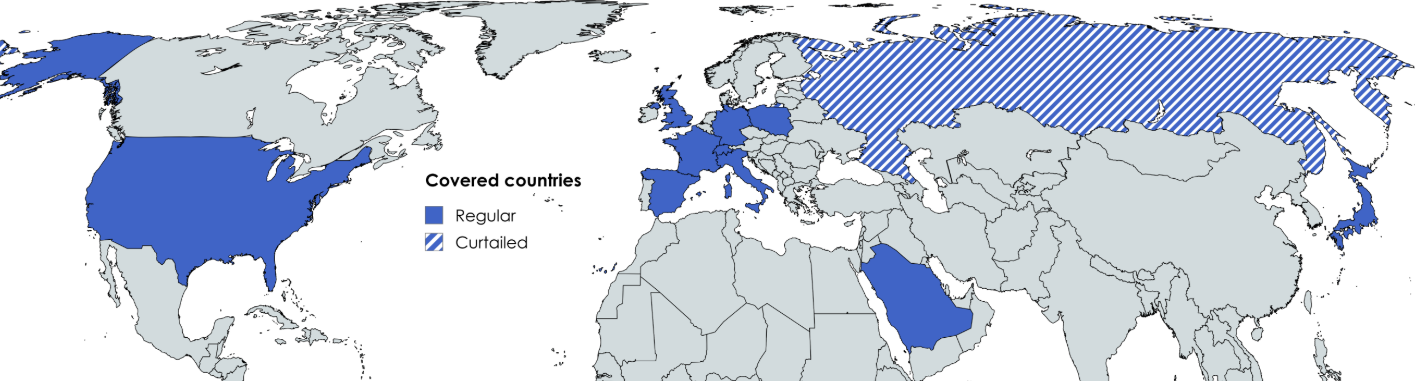
\includegraphics[width=\textwidth]{../figures/maps_participation/country_coverage_curtailed.png}} 
\end{figure}

\paragraph{Representativeness.}
The samples are stratified to be representative of the country's adult population along the following quota variables (with some exceptions\footnote{In the U.S., I also use race (4 categories) as a quota variable. In Saudi Arabia, I do not use urbanicity, but I use citizenship (Saudi vs. non-Saudi). In Russia, I do not use region nor urbanicity.}): gender, age (5 brackets), income (4), diploma (3), region (2 to 5), and urbanicity (2 to 3). Tables \ref{tab:representativeness_0}-\ref{tab:representativeness_3} in Appendix \ref{app:representativeness} show that our samples match the actual population frequencies along these dimensions, except for Saudi Arabia (where non-Saudis and non-high-school-educated people are underrepresented) and Russia (where TODO). All our results are reweighted to be fully representative of the population along our quotas (with weights trimmed between 0.25 and 4). Results aggregated at the global or European levels weigh each country in proportion to its adult population size. 

Appendix Figure \ref{fig:lmg} shows that 11\% to 17\% of the variance of our main attitudinal outcomes is explained by sociodemographic variables, and this share falls below 5\% after accounting for country and vote. In other words, even though variables such as age or diploma are sometimes significantly correlated with attitudes (see Tables \ref{tab:determinant}-\ref{tab:determinants_custom_redistr}), difference in average acceptance of a policy between (say) age groups rarely exceeds a dozen percentage points. % TODO? move to subsec:debated ?

Appendix \ref{app:pol} shows how our main attitudinal outcomes vary by political leaning. Non-voters exhibit attitudes close to the center of the politicalspectrum. Besides, attitudes are much less polarized in Japan compared to Europe and the U.S. % TODO: has polarization decreased since last paper?
Appendix Figures \ref{fig:vote_pnr_out}-\ref{fig:vote_representativeness} show how our % weighted or not TODO % TODO! US in Figure
samples compare to reality in terms of vote in the last election. While the share of declared non-voters is lower than in reality, votes along the three main political leanings are close to reality. Appendix \ref{app:vote} shows that our main results are robust to reweighting by vote. 

\paragraph{Data quality.} 
The median survey duration is 17 minutes (13 min in Russia). % Following TODO cite Stantcheva
Best practices have been used to ensure top-notch data quality. 
The questionnaire has been worded in a neutral and informative way;\footnote{At the end of the survey, 70\% of the respondents find it politically unbiased (Appendix Figure \ref{fig:survey_biased}).} tested on random people in public spaces to make sure it is correctly understood; translated by professional translators, with figures converted into national currencies, and double-checked by native speakers.

Of all respondents who started the questionnaire, only TODO \% dropped out. TODO respondents were allowed to pursue the survey (as their quotas were not full) and did not drop out.  The final sample is obtained after excluding of this extended sample TODO \% of respondents for suspicion of low quality: \% for failing an attention test and \% for answering the questionnaire in less than 6 min (including \% for both reasons). Appendix \ref{app:attrition} checks for differential attrition and Appendix \ref{app:extended} shows that our main results replicate on the extended sample. 
% TODO: feedback field

Whenever possible, the order of question items is randomized. Appendix \ref{app:order} studies the effect of item order on answers. The item order generally has a significant but small effect (2 to 10~p.p.). The size of the effect help identify questions for which opinions are strongly held (e.g. the preference of a sustainable scenario over the status quo) \textit{versus} weakly held (e.g. the preferred amount of climate finance). % crystallized, well-formed, consolidated, stable, ambivalent

Appendix \ref{app:comparison} compares the answers of two attitudinal questions asked in other surveys: the overall averages differ by 2 to 4~p.p. and their cross-country correlation is high: .70 \citep{global_nation_global_2023} to .86 \citep{cappelen_majority_2025}. 

\paragraph{Incentives.}
The questionnaire includes three incentivized questions, each awarded with a \$100 prize for one randomly drawn winner. First, a comprehension question on the Global Climate Scheme (GCS) checks whether respondents have understood the policy's cost. % TODO: support among those who haven't understood
Second, a donation lottery where respondents choose what part of the prize they would donate to a reforestation NGO, should they win the lottery. Third, a question on the perception of the actual support for the GCS, which rewards a correct guess.

\paragraph{Survey structure.}
While Appendix \ref{app:questionnaire} provides the full questionnaire, Figure \ref{fig:flow} depicts the survey flow with all random branches. The various treatments are all independent and uniformly distributed. Whenever there is a treatment, the acceptance levels reported are computed on the control group. Appendix \ref{app:placebo} runs placebo tests to check whether earlier treatments have an effect on unrelated outcomes. 
% # 2. survey_flow
\begin{figure}[h!]
    \caption[Survey flow]{Survey flow.
    }\label{fig:flow}
    \makebox[\textwidth][c]{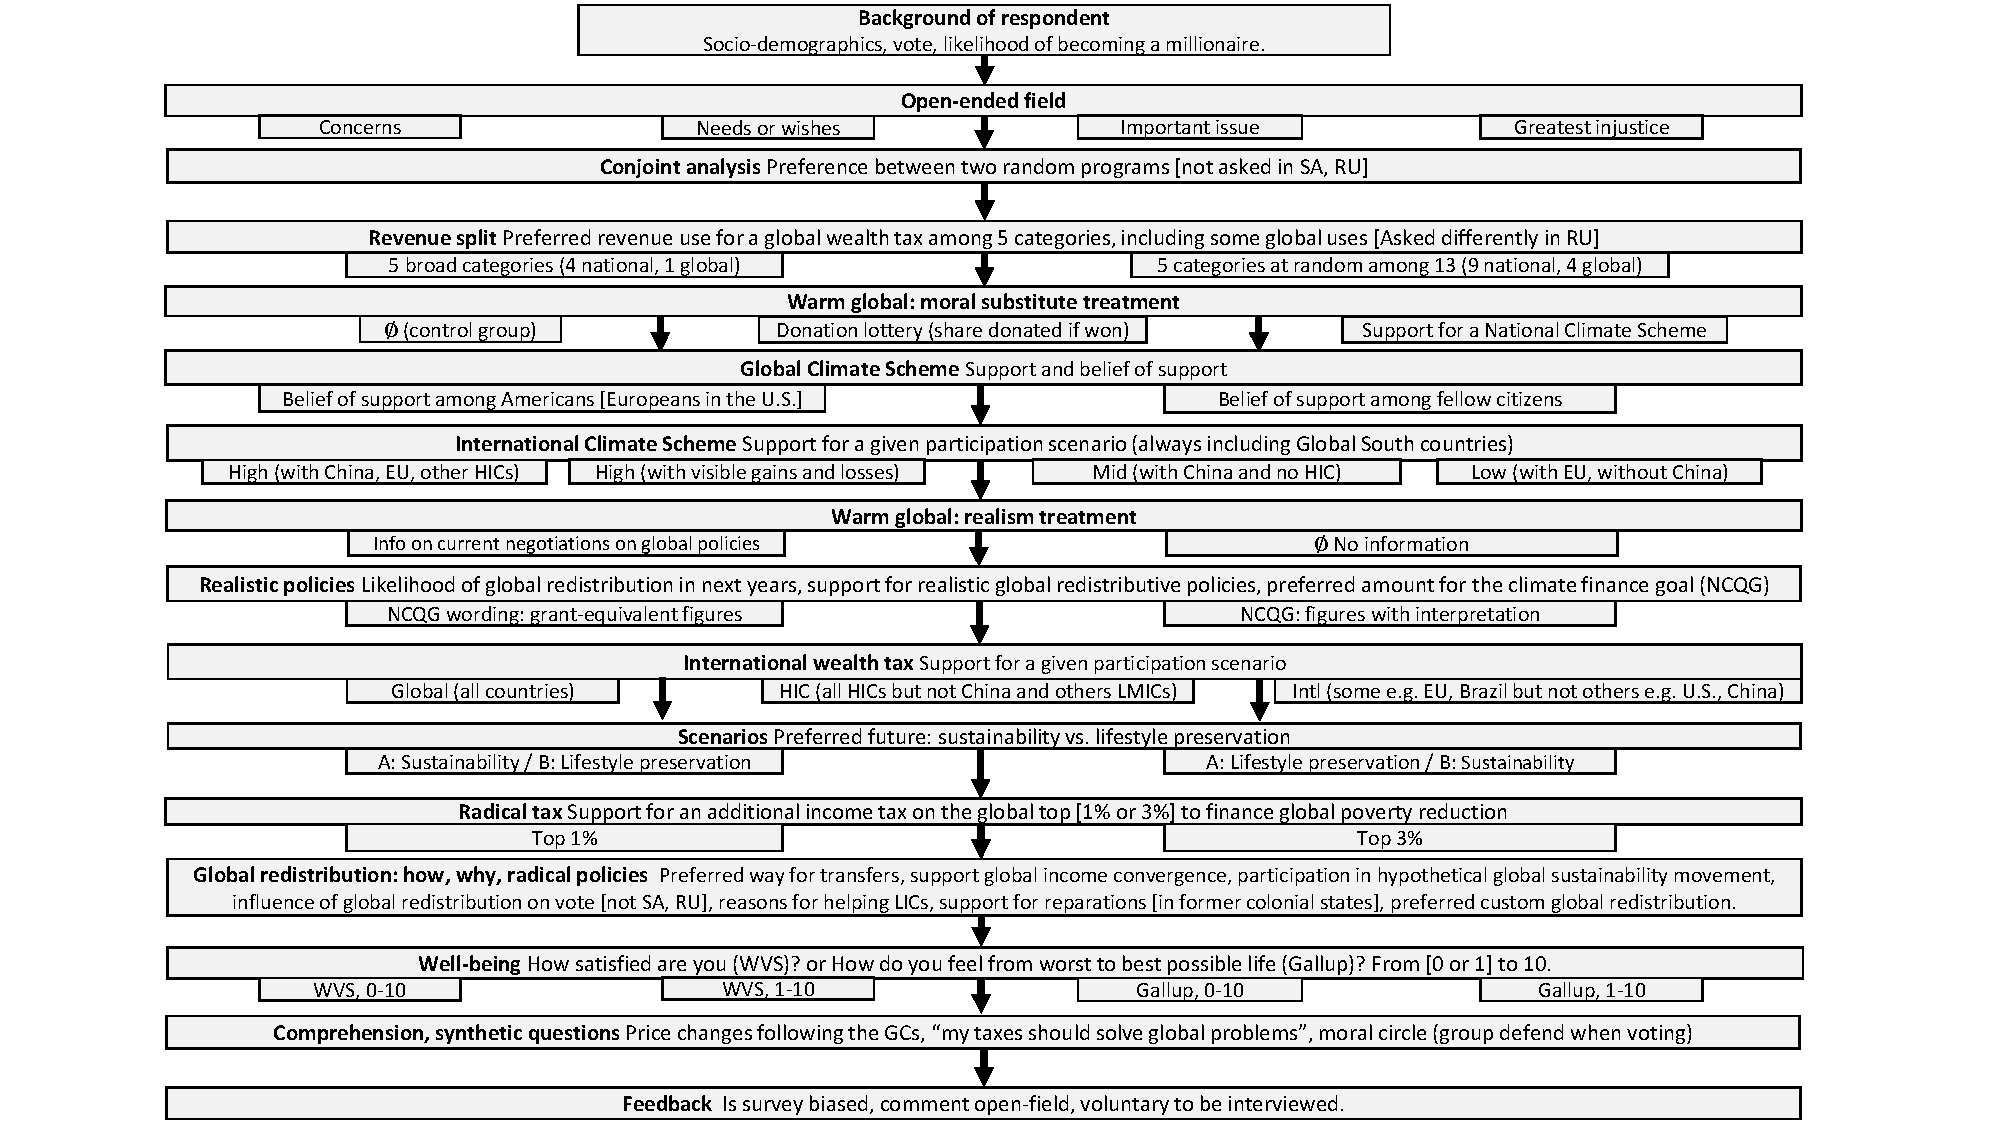
\includegraphics[width=\textwidth]{../figures/questionnaire/survey_flow.pdf}} 
\end{figure}

After sociodemographic characteristics, the questionnaire starts with broad questions to grasp the prioritization and salience of global solidarity before the respondents can understand the survey's topic. First, open-ended fields on either their main concerns, wants, issues of interest, or perceived injustices. Second, a conjoint experiment where respondents have to select their preferred political program, or abstain. Both programs are random: each policy (or absence of policy) in five policy domains is taken at random from a pool of policies prominent in the country's public debate. Third, respondents are asked to allocate the revenue of a global wealth tax between five (national or global) spending items. 

Then come attitudinal questions on the main policies studied: a \textit{Climate Scheme} at the national, global, or international level; an international wealth tax funding low-income countries; and ten plausible global solidarity policies. These questions include treatments that vary the international coverage of policies or test for warm glow. 

The last part of the questionnaire explores attitudes towards more radical global redistribution scenarios and include more sophisticated questions, such as an interactive task where respondents can choose their preferred custom redistribution of global incomes by manipulating sliders. 

Finally, the survey concludes with a comprehension question, synthetic questions (e.g. on moral circle) and a feedback field.

\paragraph{Pre-registered hypotheses and data availability.}
The project is approved by the CIRED institutional review board (IRB-CIRED-2025-2) and %is approved by IRB at Harvard University (IRB21-0137), and 
was preregistered in the Open Science Foundation registry (\href{https://osf.io/7mzn4}{osf.io/7mzn4}). The study did not deviate from the registration: the questionnaires and the hypotheses tests used are the ones \href{https://osf.io/j5scn}{specified \textit{ex ante}}. All data and code as well as figures of the paper are available on \href{https://github.com/bixiou/robustness_global_redistr}{github.com/bixiou/robustness\_global\_redistr}. 


\section{Salience and prioritization of global solidarity\label{sec:salience}}
% - People view global poverty/ineq as big injustice though not salient concern (e.g. revenue_split)
In this Section, I analyze the salience of global solidarity in undirected open-ended fields; and the prioritization of global programs in a budget allocation task.

\subsection{Top-of-mind considerations}\label{subsec:considerations}

At the beginning of the survey, respondents are randomly assigned one open-ended question among four: their main concerns, their needs or wishes, an issue important to them but neglected in public debate, or the greatest injustice of all. The questions are deliberately broad and vague to let respondents express their top-of-mind considerations without any priming. 

To analyze the answers, I automatically translated each field into English.\footnote{I used \href{https://www.onlinedoctranslator.com/en/translationform}{onlinedoctranslator.com}, which is powered by \textit{Google Translate}.} Then, I used AI and my own reading of a few hundreds answers to identify the most common concepts, from which I selected 27 categories. Then, I classified each answer into one or more of these categories, both manually (Figures \ref{fig:field_manual}-\ref{fig:injustice_field}) and automatically using AI (Figure \ref{fig:field_gpt}). Finally, I manually defined a list of 47 (conjunction of) keywords and used it to automatically classify all answers.\footnote{The list of keywords is given in Appendix TODO.} I report occurrences of the 24 most common keyword matches in Figure \ref{fig:field_keyword}. 

The three different classification methods yield consistent results but differ in accuracy. While the keyword classification allows an exact and reproducible search, the automatic search is not bound to specific words and captures more matching responses. % Although the manual classification could be less consistent than the AI one (if e.g. the interpretation of the category changes over time or among coders), 
Overall, it seems that the manual classification provides the most accurate results, with a number of matches generally between the two other methods. 
For example, to the \textit{injustice} question, 1.3\% of answers match the keywords for \textit{global inequality} and ChatGPT identifies this category in 8.5\% of answers, \textit{versus} 3.7\% according to my manual coding.\footnote{The keyword matching searches the regular expression ``global poverty|global inequal|hunger|drinking water|starv'', ignoring case. The automatic and manual classification is based on the class definition ``Inequality at the inetrnational level / Hunger or poverty in poor countries''.} 
Indeed, the AI incorrectly classifies unspecific answers like ``poverty'' in this category,\footnote{Interestingly, out of the 45 (one-word) answers ``poverty'', ChatGPT-4.1 coded only 42 of them as \textit{global inequality}, showing the lack of consistency of this classifier.} while the keyword search misses answers like ``inequality among humans''. 
Given this observation, I use the manual classification as the benchmark and the two other methods as robustness checks.

While less accurate than the classifications, wordclouds (Figure \ref{fig:wordcloud}) provide a simple visualization of the most common concepts in each question. By far, the most frequent \textit{concerns} or \textit{wishes} of respondents relate to their purchasing power, with concepts such as ``money'', ``inflation'', the ``cost of living'', or ``financial stability'' mobilized in 30\% of these fields. Within country, the share of people concerned with money decreases with income: it ranges from 21\% in the top income decile to 36\% in the bottom one. % TODO define e$gdp_pc_ppp and cor money
The next most frequent \textit{concerns} are health (or the healthcare system), far right governments (or related concepts such as ``Trump'' or ``trade tariffs''), and war (either in general or a specific one such as the Gaza war). Most \textit{wishes} are personal, with the next frequent ones related to the health or peace of mind of oneself or one's relatives. Interestingly, almost none of the responses mention relational considerations such as love, friendships, loneliness, intimate life, or the desire to have children (except for Saudi Arabia for the latter). Further research is needed to test whether the predominance of materialistic considerations stems from the context (an impersonal survey) or truly reflects people's primary thoughts. 

% # 3. keywords in fields (taken jointly)
\begin{figure}[h!]
  \caption[Wordcloud of open-ended field, per variant]{Most common concepts in open-ended fields. (Questions \ref{q:concerns_field}-\ref{q:injustice_field})} \label{fig:wordcloud} % Random answers can be found on \href{http://preferences-pol.fr/fields2025.html}{bit.ly/fields2025}
  \begin{subfigure}{.48\textwidth}
    \caption[]{``What are your main concerns these days?''}
    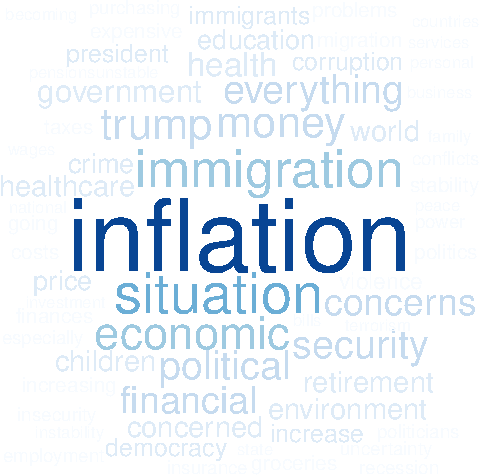
\includegraphics[height=.35\textheight]{../figures/all/concerns_field_en.pdf}
  \end{subfigure} \quad
  \begin{subfigure}{.48\textwidth}
    \caption[]{``What are your needs or wishes?''}
    
\includegraphics[height=.35\textheight]{../figures/all/wish_field_en.pdf}
  \end{subfigure}
  \begin{subfigure}{.48\textwidth}
    \caption[]{``What according to you is the greatest injustice of all?''}
    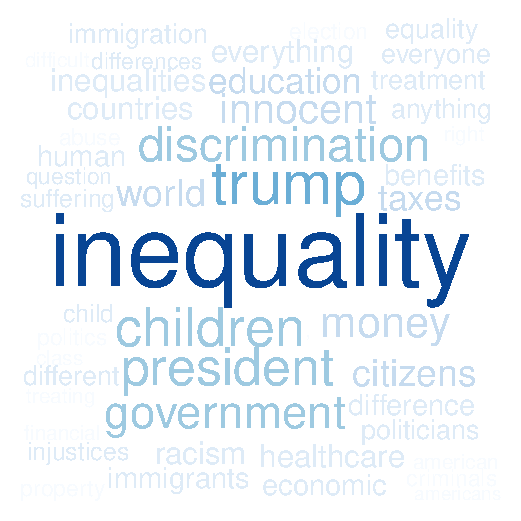
\includegraphics[height=.35\textheight]{../figures/all/injustice_field_en.pdf}
  \end{subfigure} \quad
  \begin{subfigure}{.48\textwidth}
    \caption[]{``Can you name an issue that is important to you but is neglected in the public debate?''}
    
\includegraphics[height=.35\textheight]{../figures/all/issue_field_en.pdf}
  \end{subfigure} 
\end{figure}

Asked about the greatest \textit{injustice}, the most frequent answers relate to ``inequality'' or ``poverty'', with 19\% of occurrences (28\% in Europe but only 9\% in the U.S.). It is unclear whether these respondents think about inequality in their own country or at the global level, as only 13\% of them mention a geographical scope. A hint is that, among them, 2\% mention their own country \textit{versus} 11\% the global level (or Global South issues such as ``clean water'' or ``starvation''), with Italians and Poles the most prone to mention the global level and Japanese the least. The next most common answers relate to ``discrimination'' (based on gender, race, or sexual orientation), ``violence'' or ``wrongful convictions'' (many respondents denounce unjustly sentenced innocents), or their country's ``welfare State'' (with people either criticizing the lack of public services or excessive welfare for underserving people). 

Asking people for ``an issue important to them but neglected in the public debate'' fails to uncover unusual topics. 20\% of respondents are not able to find such an issue. Although ``immigration'' is the most frequent word according to the wordcloud, only 5\% of respondents refer to this issue, which comes after ``public services'', the ``cost of living'', or the ``environment''. That most topics mentioned are already highly publicized suggests that the public debate either reflects or shapes what people have in mind. % ``taxes'' or the ``welfare State'' (12\%), the ``healthcare system'' (9\%), the ``cost of living'' (9\%), and the ``environment'' (6\%).

Reading and coding each field one by one took about 30 hours, but it was worth it: not only does it result in an arguably more accurate classification; it also helped me grasp people's ways of thinking first hand. For example, most people reason from their own perspective (e.g. ``my pension is too low'', ``I want to buy a house'') and do not refer to the broader picture or to political reforms. To get a sense of people's own words, a random display of responses can be found on \href{http://preferences-pol.fr/fields2025.html}{bit.ly/fields2025}.

% Interestingly, the topics vary significantly across countries. Here are my impressions of each country's slant. Compared to other countries, the concepts overrepresented in each country are as follows:
% \begin{itemize}
%   \item France: insecurity, holidays or free time, the public deficit, equality, gender equality;
%   \item Germany: old age poverty, immigration, the return of growth or the economic situation, free time, war (in Europe), bureaucracy;
%   \item Italy: health, serenity or peace of mind, war, work stress and free time, world hunger, feminicides; 
%   \item Poland: war, inequality, holidays, honesty, disabled people;
%   \item Spain: ``health, money and love'', housing, corruption, water access, global poverty, squatters;
%   \item the UK: the cost of living, immigration, having a comfortable life, mental health, the holocaust, roads dangerous for driving, being unjustly imprisoned, cut in winter fuel allowance;
%   \item Switzerland: equality, immigration, gender equality;
%   \item Japan: the level of pensions, a cut on the consumption tax, the price of rice, the declining birth rate, childcare support, reducing the number of parliament members, foreigners' preferential treatment, excessive social assistance or the lack of reward for hard work, stock prices;
%   \item Saudi Arabia: hobbies such as sports or soccer, the willingness to become millionaire (or billionaire), one's business project, buying a house, their car, that they are satisfied with their income, ``self-injustice'' or sin, raising children, Palestine, orphan's oppression, travels;
%   \item the U.S.: the economy, Trump, breaches to the Constitution, abortion, and gun control.
% \end{itemize}
Interestingly, the topics vary significantly across countries. Here are my impressions of each country's slant. Compared to other countries, the concepts overrepresented in France are: insecurity, holidays or free time, the public deficit, equality, or gender equality; in Germany: old age poverty, immigration, the return of growth or the economic situation, free time, war (in Europe), and bureaucracy; in Italy: health, serenity or peace of mind, war, work stress and free time, world hunger, and feminicides; in Poland: war, inequality, holidays, honesty, and disabled people; in Spain: ``health, money and love'', housing, corruption, water access, global poverty, and squatters; in the UK: the cost of living, immigration, having a comfortable life, mental health, the holocaust, roads dangerous for driving, being unjustly imprisoned, and cut in winter fuel allowance; in Switzerland: equality, immigration, and gender equality; in Japan: the level of pensions, a cut on the consumption tax, the price of rice, the declining birth rate, childcare support, reducing the number of parliament members, foreigners' preferential treatment, excessive social assistance or the lack of reward for hard work, and stock prices; in Saudi Arabia: hobbies such as sports or soccer, the willingness to become millionaire (or billionaire), one's business project, buying a house, their car, that they are satisfied with their income, ``self-injustice'' or sin, raising children, Palestine, orphans' oppression, and travels; in the U.S.: the economy, Donald Trump, breaches to the Constitution, abortion, and gun control.

% TODO? Correlations with sociodemos?
% Our topic of interest, \textit{global inequality}, does not emerge as an issue salient to most people. It is rarely mentioned as a neglected \textit{issue} or as a \textit{concern}, contrary to international issues such as war, climate change, or the rise of the far right. And while \textit{global inequality} is mentioned as frequently as these other international issues in terms of \textit{injustice}, addressing it seldom appears as a \textit{wish}. Indeed, most considerations relate to issues that directly affect oneself or one's family, and political considerations (regarding e.g. public services, pensions or taxes) are often framed at the national level. %are self- or family-centered.
Our topic of interest, \textit{global inequality}, does not emerge as an issue salient to most people. Indeed, most considerations relate to issues that directly affect oneself or one's family, and political considerations (regarding e.g. public services, pensions or taxes) are often framed at the national level. \textit{Global redistribution}almost never appears as a \textit{wish}. Furthermore, \textit{global inequality} is rarely mentioned as a neglected \textit{issue} or as a \textit{concern}, contrary to international issues such as war, climate change, or the rise of the far right. However, it is mentioned as frequently as these other international issues in terms of \textit{injustice}. 
To sum up, the low salience of global solidarity may explain why this topic fails to mobilize political forces despite it being referred to as a just cause and it being accepted by majorities (as shown below). 

\subsection{Prioritization of public spending items}\label{subsec:revenue_split}

\cite{fabre_majority_2025} finds that 58\% of US-Americans and 71\% of Western Europeans would support a global tax on millionaires funding low-income countries (LICs), with only 26\% and 14\% opposing it; that around half of them would prefer to allocate half (rather than none) of the revenue from a global wealth tax to LICs; and that, on average, respondents prefer to allocate 33.4\% of such revenue to LICs (\textit{versus} domestic healthcare and education). 
% \cite{fabre_majority_2025} uses two random variants to study the preferred use of revenue from a global wealth tax between infrastructure and public services \textit{in
% low-income countries} \textit{versus} \textit{domestic} healthcare and education. The ``binary'' variant shows that around half of US-Americans and Western Europeans prefer to allocate half (rather than none) of the revenue to low-income countries. The ``continuous'' variant shows that the median respondent prefers to allocate 30\% of the revenue to low-income countries (LICs).
In other words, while most people would prefer a globally redistributive tax to the status quo, the more leeway they are granted to allocate the revenue from such a tax, the less they would allocate to LICs. The greatest leeway tested by \cite{fabre_majority_2025} let the respondents select their preferred share for LICs \textit{versus} one alternative spending item, and the average preference was 33.4\%, that is 67\% of an equal split. % \footnote{The greatest leeway possible would be an open-ended field, but its interpretation would be challenging as answers that do not specify the geographical scope would be equivocal.}
Naturally, one expects respondents to split the revenue between all desirable spending items, so that the revenue allocated to one item depends on the number of items. Therefore, if LICs compete with not one but several national items, the share allocated to LICs is expected to diminish. If this share is less than 67\% of the equal split, it would mean that \citep{fabre_majority_2025} overestimated the prioritization of LICs, e.g. or due to an excessive salience of LICs when only one alternative is proposed, or due to the domestic alternative --healthcare and education-- not being the most desired. Conversely, if several items relate to a global issue, the total of ``global spending'' should increase. If global spending increases by less than the proportionate amount for the number of global items, it could mean that people view global items as a single entity, but that some domestic issues were missing from the binary version.

To test whether results from \citep{fabre_majority_2025} gave an accurate picture of the % relative
prioritization of global spending as well as to uncover the prioritization of different global causes, I conduct a revenue allocation task with five spending items. 
In each of the two variants of this task, respondents use sliders to allocate the revenue of a fictive global tax of wealth (in excess of \$5 million, at a rate of 2\%), after being informed of the revenue the tax would collect in their country (from \$1 billion in Poland to \$514 in the U.S.) \textit{versus} in all LICs combined (\$1 billion). 

In the variant \textit{Few}, one global item (``Education, Healthcare and Renewable energy in LICs'') competes with four domestic ones. %(``Education and healthcare'', ``Social welfare programs'', ``Reduction in the income tax'', ``Reduction of the deficit''). 
In every country, the most prioritized item is ``Domestic: Education and healthcare'', with an average preferred share of 26\% (Figures \ref{fig:split_few_bars_nb0}, \ref{fig:split_few}). The global item is the least prioritized overall, at 17.5\% (from 14\% in Japan to 21\% in Saudia Arabia and Spain). However, global spending is 31\% higher than the expected 13.4\% (that is 66.8\% of % an equal split of % TODO stat test
20\%)\footnote{If one restricts the comparison to the countries surveyed by \citep{fabre_majority_2025}, the global item is allocated 17.8\%, that is 34\% more than expected. The most credible explanation for outperforming expectations is that the domestic item chosen by \citep{fabre_majority_2025} was the preferred one. Indeed, the global item is allocated 68\% of the ``Domestic: Healthcare and Education'' share, almost exactly as expected.} and only 13\% of the respondents do not allocate any revenue to it (Figure \ref{fig:split}). 

%While these results reveal large acceptance of allocating a substantial share of the revenue from a global tax to LICs, this may result from framing the question with only two spending items (domestic \textit{versus} LICs). 

% # 4. revenue_split: country_comparison/split_main_means_nolegend + country_comparison/split_main_nb0_nolabel
\begin{figure}[h!]
  \caption[Preferred split of revenue of an international wealth tax]{Preferred split of revenue of an international wealth tax. The first two items are from the variant \textit{Few} with 5 fixed items (the \textit{Global} one and the most preferred one are displayed); the last four items are from the variant \textit{Many} with 5 items taken at random out of 13 (the 4 \textit{Global} ones are displayed). \hfill (Questions \ref{q:revenue_split_few}-\ref{q:revenue_split_many})} \label{fig:split}

  % \begin{subfigure}{.45\textwidth}
  %   \caption[]{Average preferred allocation (in \%).}
  %   \begin{flushleft}
  %   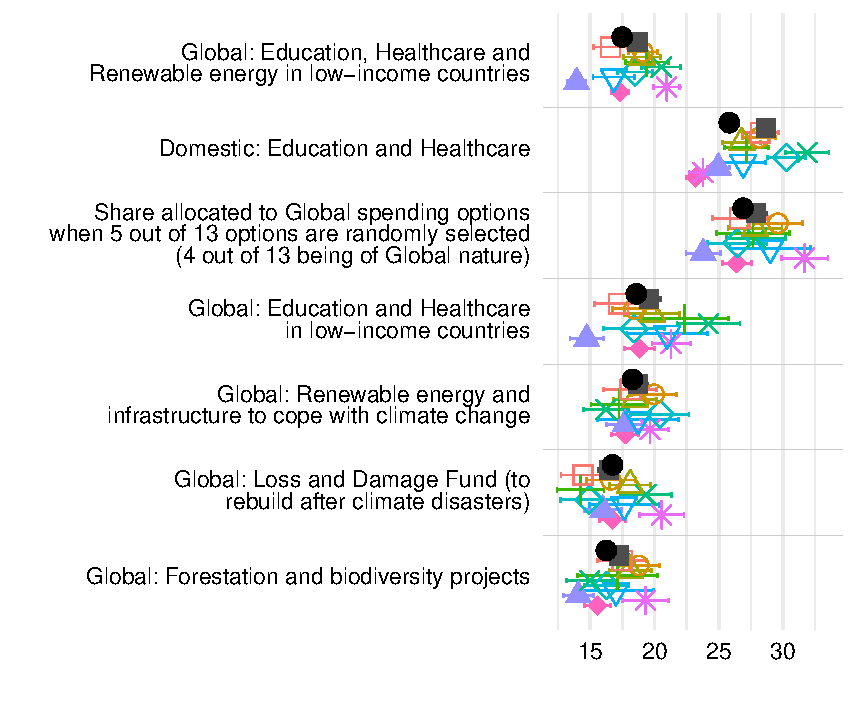
\includegraphics[height=.36\textheight]{../figures/country_comparison/split_main_means_nolegend.pdf}\end{flushleft}
  % \end{subfigure} 
  % \begin{subfigure}{.55\textwidth}
  %   \caption[]{Share of respondents allocating 0 revenue (in \%).} 
  %   \begin{flushright}
  %   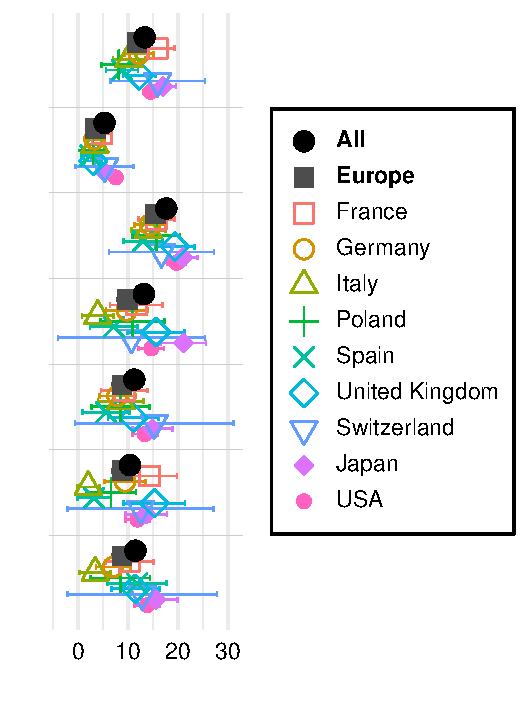
\includegraphics[height=.36\textheight]{../figures/country_comparison/split_main_nb0_nolabel.pdf}\end{flushright}

\begin{subfigure}{.62\textwidth}
    \caption[]{Average preferred allocation (in \%).}
    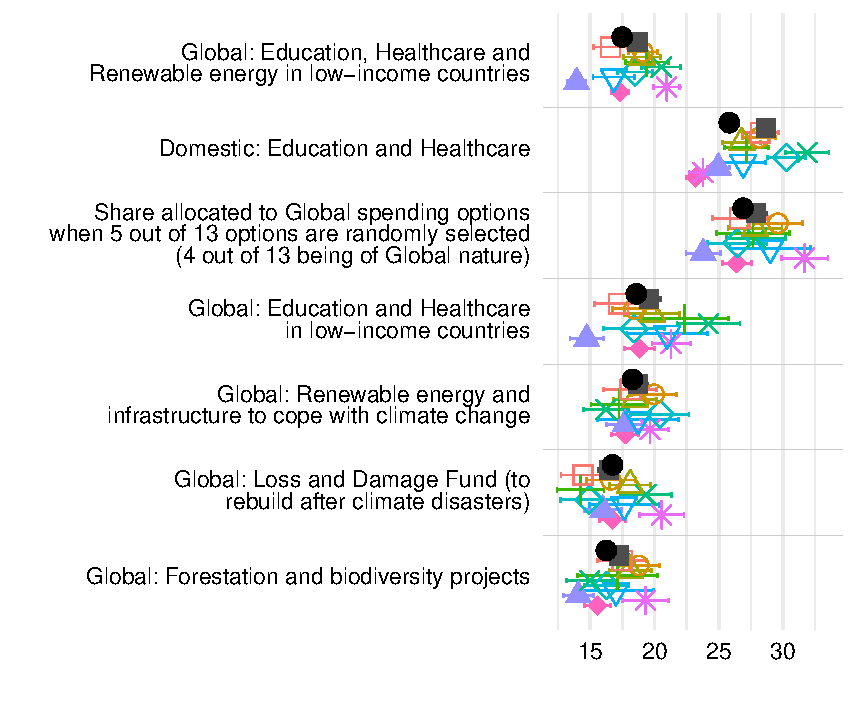
\includegraphics[height=.38\textheight]{../figures/country_comparison/split_main_means_nolegend.pdf}
    \end{subfigure} 
  \begin{subfigure}{.38\textwidth}
    \caption[]{Share of respondents allocating 0 revenue (in \%).} 
    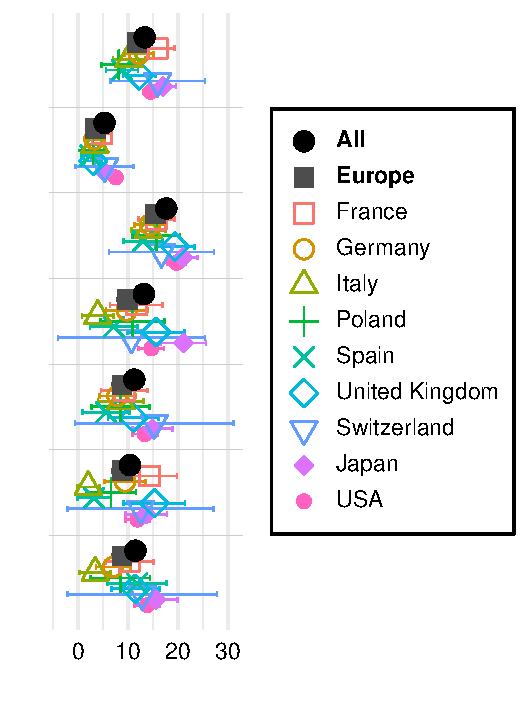
\includegraphics[height=.38\textheight]{../figures/country_comparison/split_main_nb0_nolabel.pdf}

  \end{subfigure}
\end{figure}

In the variant \textit{Many}, five items are selected at random among a pool of four global and nine domestic items. While domestic healthcare (27\%) %(27.0\%) 
and education (23\%) %(22.5\%) 
are the most prioritized items, global ones obtain an average ranging from 17\% %16.5\% 
for ``Forestation and biodiversity projects'' to 19\% %18.6\% 
for ``Education and Healthcare in LICs'' (Figures \ref{fig:split}, \ref{fig:split_many}-\ref{fig:split_many_global_mean}). On average, there are 1.5 global items and they are allocated 26.9\% of the revenue, which again corresponds to 17.5\% per global item. Interestingly, there is no significant correlation between the number of global items and the average allocation per global item. % TODO table
% TODO: Russia

In other words, the revenue allocation tasks validate and confirm the results from \citep{fabre_majority_2025}. Most people would like to use a substantial share of the revenue from a global wealth tax to financing sustainable development in LICs, even though global spending is somewhat less prioritized than domestic spending. 


\section{Acceptance of international policies in function of country coverage\label{sec:coverage}}
% - Strong support for global tax / GCS even with partial participation

While acceptance of global climate or redistributive policies is widespread \citep{fabre_majority_2025,cappelen_majority_2025}, acceptance may drop if policies are not truly \textit{global} but only \textit{international}, i.e. if key countries such as China, Russia or the U.S. do not participate. Indeed, people may be concerned by a domestic loss of competitiveness that could result from the expatriation of taxpayers to low-tax jurisdictions; or by an unfair burden-sharing if non-cooperating countries free-ride on decarbonization or funding sustainable development. % TODO: cite Gampfer, Carlsson, Bechtel Scheve 2013 May also depend on which countries are in
In this Section, I uncover the acceptance of globally redistributive policies depending on the coalition of countries that would implement them. I study in turn a carbon price and a wealth tax.

\subsection{International Climate Scheme}\label{subsec:ics}

% NB: I chose to present GCS on control. Trade-off between presenting control results (not contaminated by treatment though less precise) and overall results (more comparable to ICS as those mix treated and control, though less comparable to NCS). I prioritized presenting results for themselves rather than for comparison with ICS.

\paragraph{Presentation of the schemes.} ``Cap and dividend'' is a reference climate policy, % TODO cite
whereby fossil fuel companies at the source of emissions must buy emission permits on a carbon market, with the revenue from carbon pricing rebated equally to individuals. The limited and declining number of emission permits guarantees that emissions are capped according to the climate objective. As polluting companies pass the cost of emission permits down the value chain, the carbon price is ultimately paid by consumers, in proportion to their carbon footprint. Meanwhile, the equal cash transfer (or ``dividend'') offsets price increases for the average consumer. Those with a carbon footprint higher than average financially lose and those with a lower carbon footprint (who are on average poorer) financially gain. 
% explanation cap & dividend

Using simple \textit{Yes}/\textit{No} questions, I test the acceptance of three types of ``cap and dividend'' (or ``Climate Scheme'') policies, that differ by the geographical scope: the National, Global, and International Climate Schemes (Figures \ref{fig:ics}, \ref{fig:ncs_gcs_ics}). While average consumers in a high-income country are financially unaffected by the National Climate Scheme (NCS), they lose out in the Global and International versions, since their carbon footprint is larger that the world (or climate coalition) average. 

The National Climate Scheme (NCS) is accepted by 66\% of respondents (ranging from 56\% in Poland to 88\% in Saudi Arabia). 
% majority support NCS (TODO? cite Douenne & Fabre? Bergquist?)
% TODO? say asked only to one-third?

\paragraph{The Global Climate Scheme.} Before presenting the Global Climate Scheme (GCS), respondents are prompted to be attentive with the incentive that they may win a \$100 lottery prize if they correctly answer a comprehension question at the end of the survey. 
When presented the Global Climate Scheme (GCS), respondents are informed that the cash transfer would lift 600~million people out of extreme poverty, and the cost to them is made salient. Respondents are informed of the amount of the cash transfer, as well as the price increases and the net cost to the average person in their country (e.g. 2\% price increases and a net cost of \$90 per month in the U.S., or 2\% and \euro{}45 per month in Germany).%
\footnote{The computations use a carbon price of \$95/tCO$_\text{2}$. For Russia, Saudi Arabia, and the U.S., computations assume universal country coverage and the cash transfer is \$35 per month. 
For Europe and Japan, the net loss is computed in a non-universal but \textit{High} participation scenario, which implies a lower cash transfer (\euro{}20 per month) and a higher net cost (by about \$10 per month) since the coalition's average carbon footprint is lower than the world average.} 
The GCS is accepted by 57\% of respondents (from 48\% in Russia to 85\% in Saudi Arabia). The salience of costs in the GCS question may explain the somewhat lower support for the GCS compared to the NCS.%
\footnote{Support for the GCS is also around 10~p.p. lower than in \citep{fabre_majority_2025}. There may be different reasons for that: attitudes may have changed in the two years interval; I added the information on the price increases, which allows respondents to make an estimate of the cost to them (rather than to their average fellow citizen)%; and the framing might have been slightly confusing in the earlier survey as the GCS was presented on the same page as a national redistribution scheme TODO? put back? 100 countries instead of 60%?
.} 

\paragraph{Pluralistic ignorance.} 
After the support for the GCS, respondents are asked in an incentivized way about their belief concerning the actual support, either in their country or in the U.S. (Figure \ref{fig:ncs_gcs_ics})\footnote{US-Americans are asked about either their country or the EU. In Russia, I was not allowed to enquire about beliefs in a foreign country.} In every country, for any variant of the question, actual support is underestimated. On average, the support in one's own country is underestimated by 14~p.p. and the support in the U.S. by 18~p.p. In Japan and in European countries, the underestimation is more severe, in the sense that most people wrongly believe that the GCS does not garner majority support in their country. Such pluralistic ignorance might explain why politicians do not dare proposing global climate justice policies. % TODO? cite Andre et al?

\paragraph{International Climate Scheme.}
To test how country coverage influences the support for the International Climate Scheme (ICS), respondents are randomly assigned to one of four variants. Respondents can visualize the country coverage on a map (see examples in Figure \ref{fig:ics_maps}), where their own country is stripped to denote its potential participation. They are also informed of the number of countries that would participate in the assigned scenario, their share of world emissions, and the list of these countries or world regions. 
% 5c.
\begin{figure}[h!]
\caption[Example maps of the International Climate Scheme]{Example maps of the International Climate Scheme question. (Question \ref{q:ics_support}).} \label{fig:ics_maps}
\begin{subfigure}{.49\textwidth}
  \caption[]{\textit{Low} variant for the U.S.}
  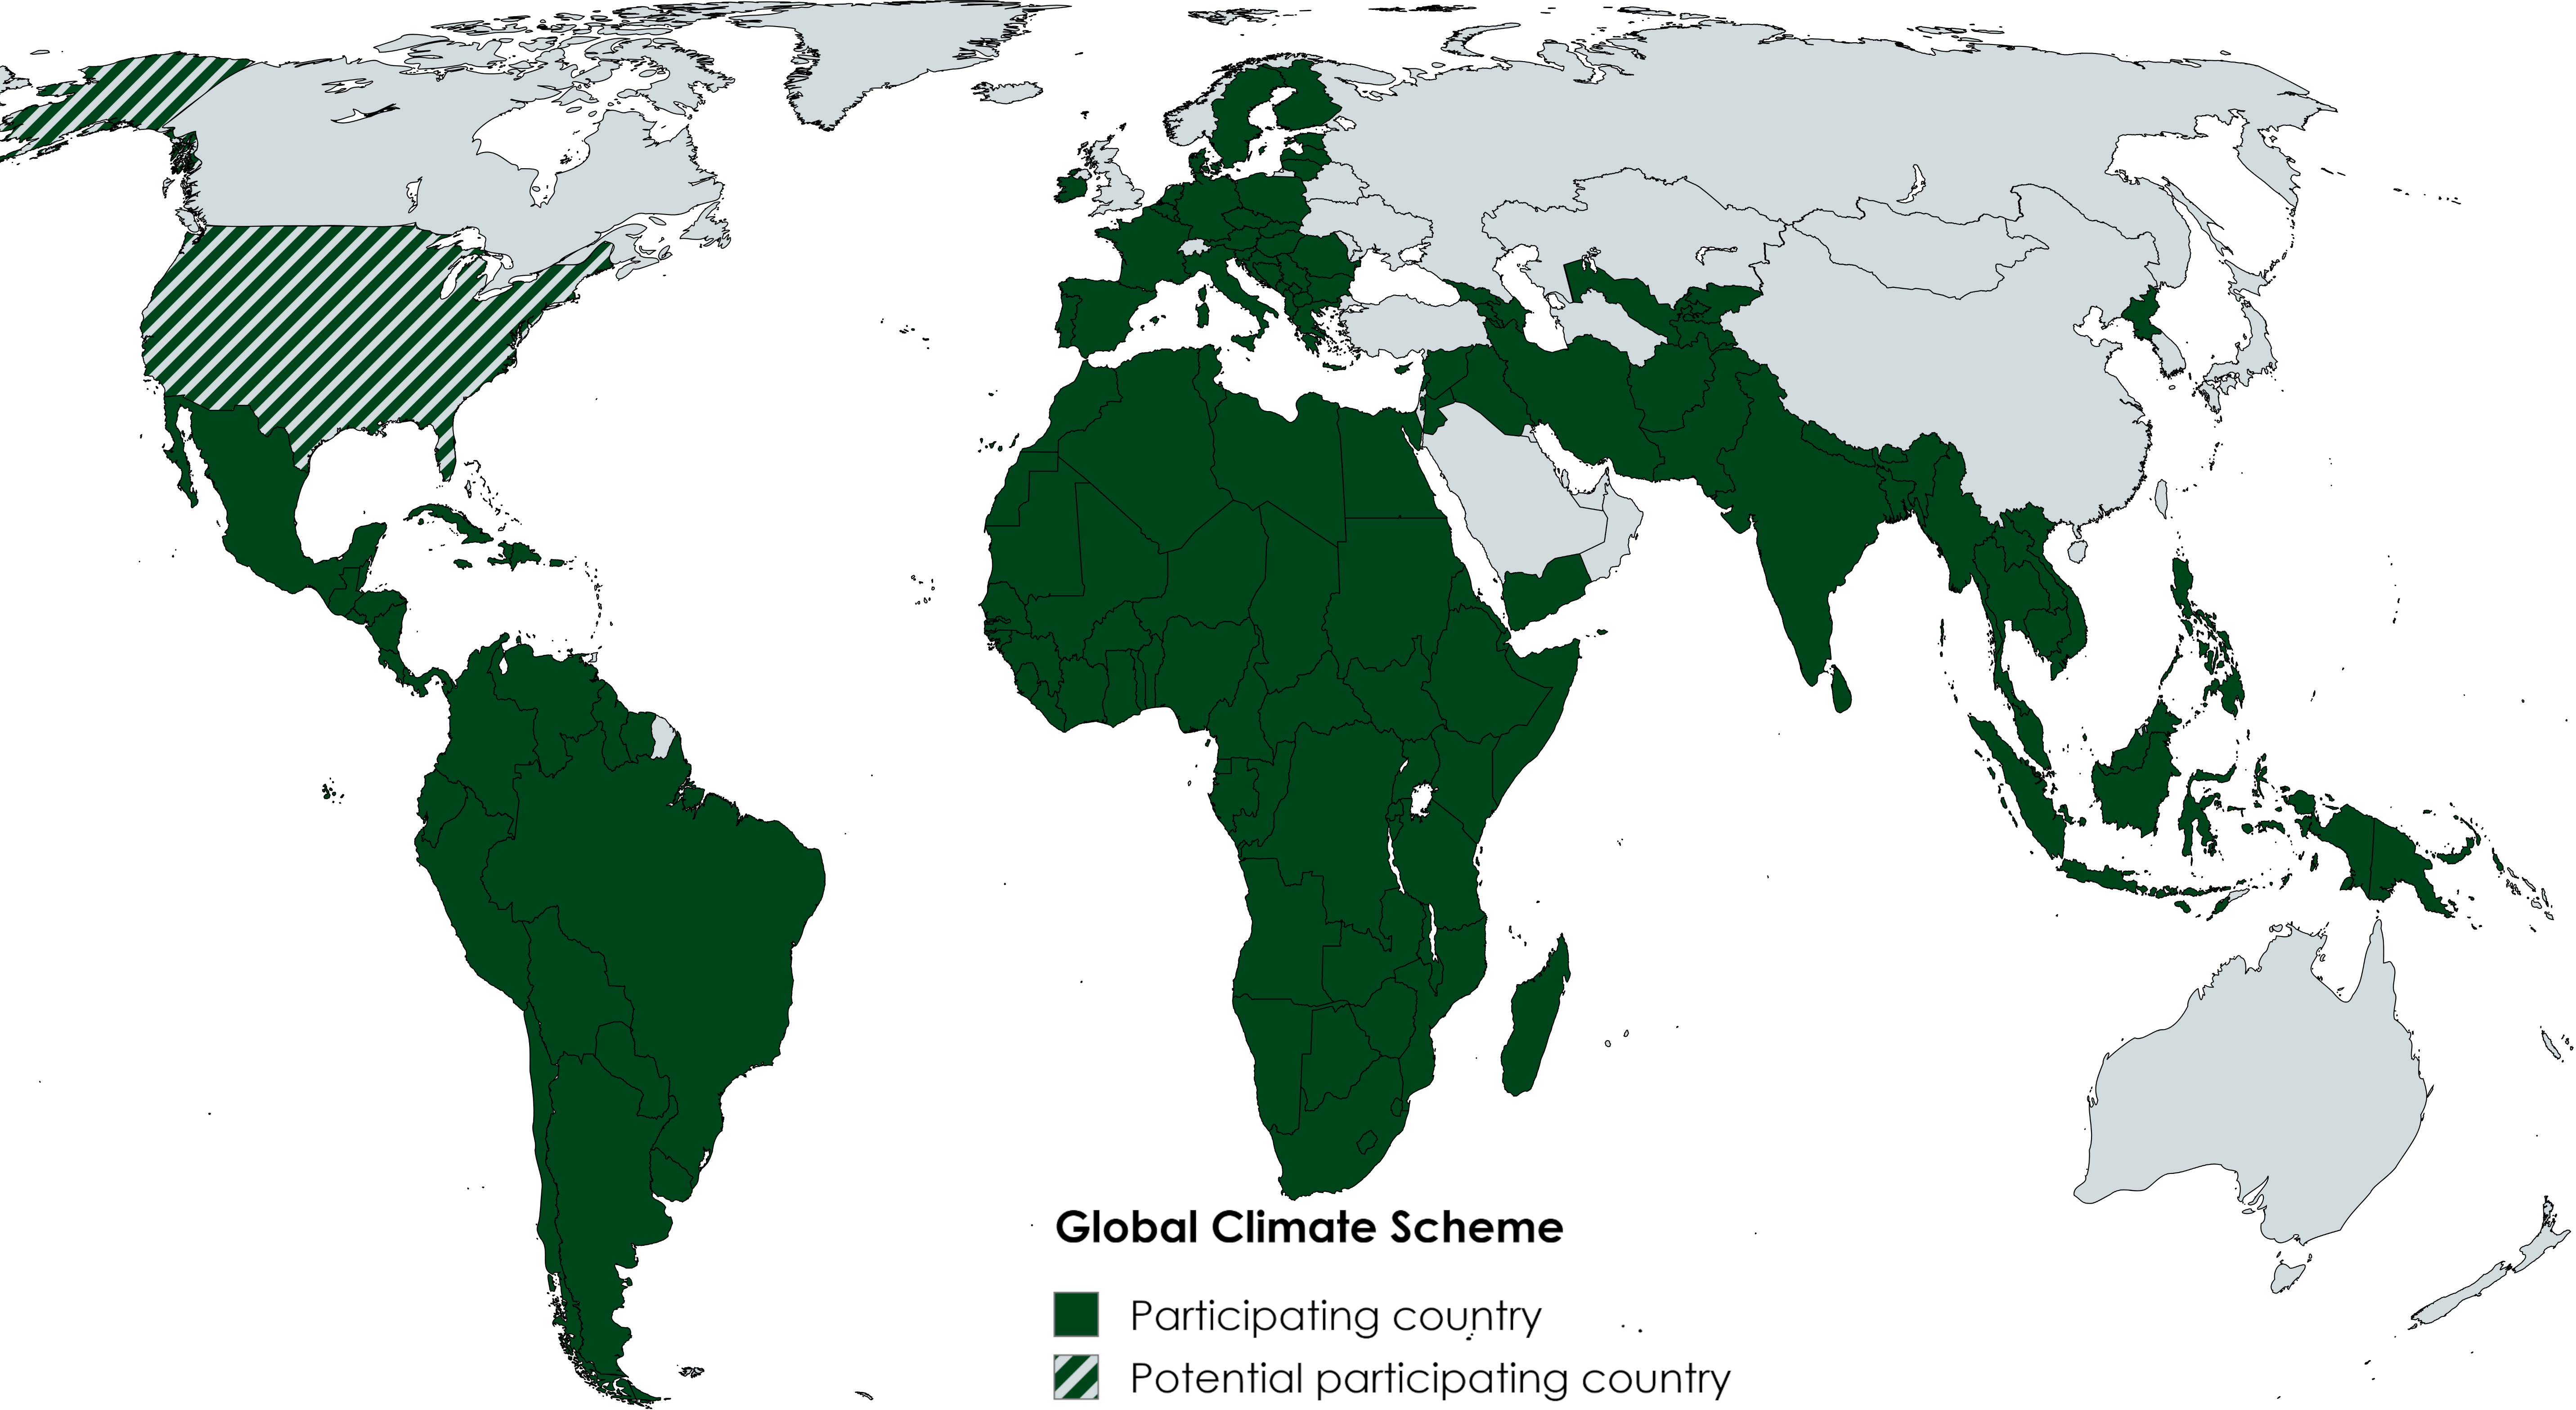
\includegraphics[height=.49\textwidth]{../figures/maps_participation/GCS_low_EN.png}
\end{subfigure} 
\begin{subfigure}{.49\textwidth}
  \caption[]{\textit{High color} variant for EU countries.}%\begin{flushright}
  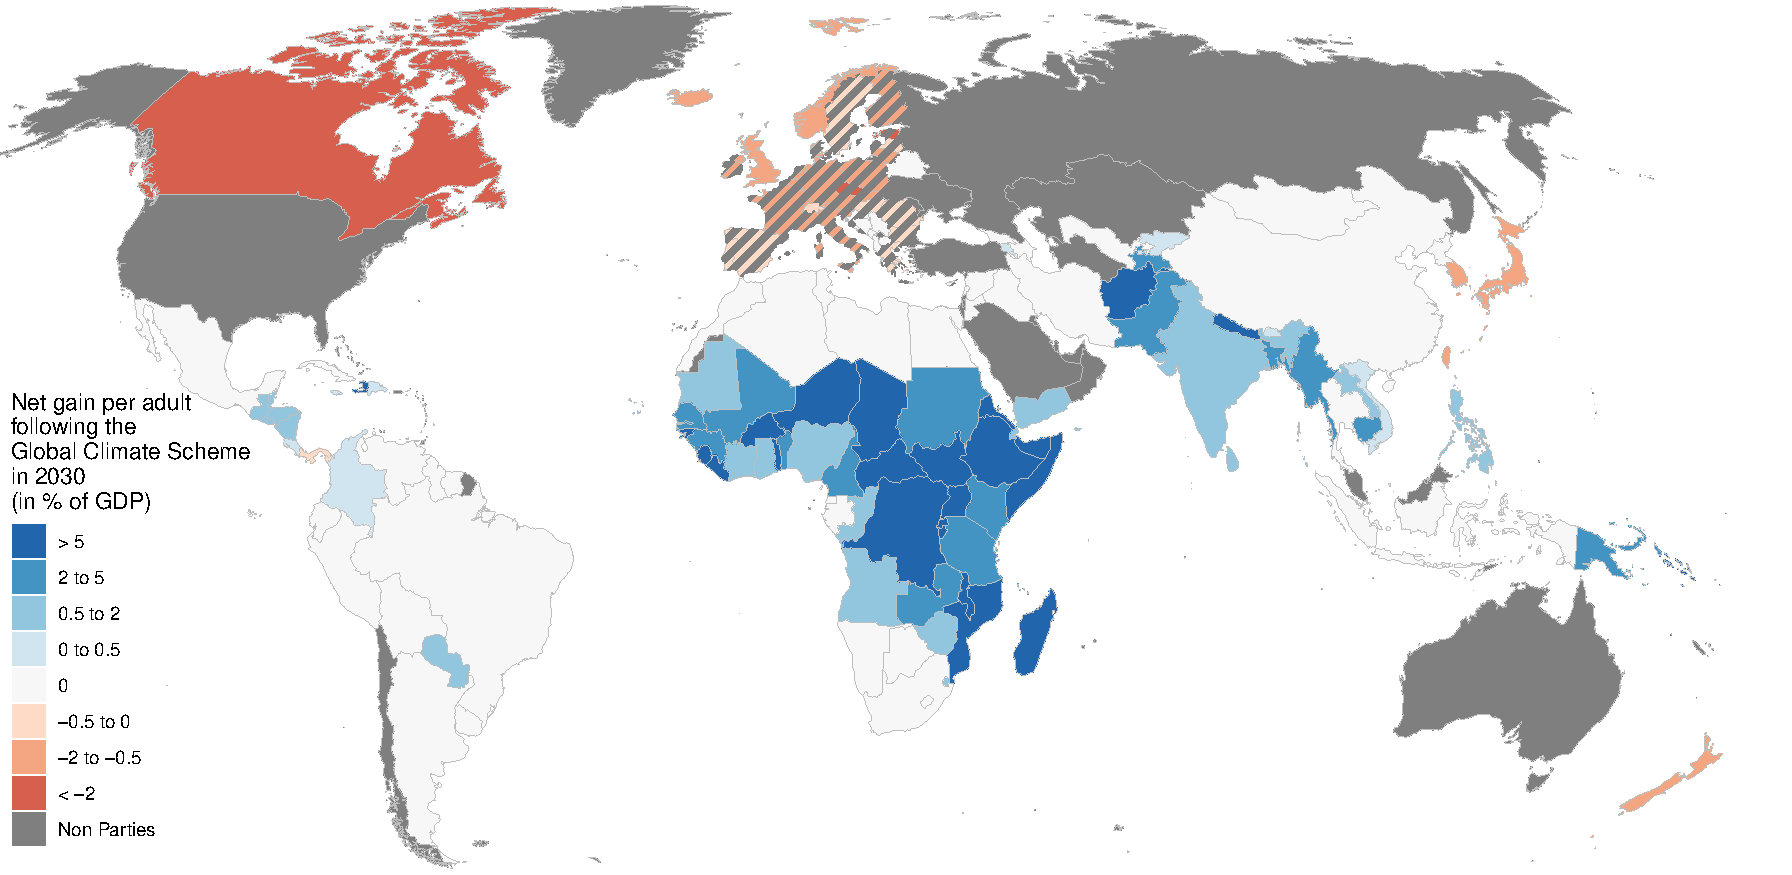
\includegraphics[height=.49\textwidth]{../figures/maps_participation/GCS_high_color_EU.pdf}%\end{flushright}
\end{subfigure}
\end{figure}

The \textit{Mid} scenario covers 56\% of world emissions, with the participation of China and Global South countries. The \textit{Low} replaces China by the EU and covers 33\% of emissions. The \textit{High scenario} adds various high-income countries to the \textit{Mid} scenario, including the EU, Japan, Canada, and South Korea; covering 72\% of emissions. The last variant, \textit{High color}, combines the \textit{High} participation scenario with a colored map that displays not only the country coverage, but also the net gain or cost for each country, with China appearing as neither gaining nor losing from the policy.\footnote{In a standard cap and dividend, China should be losing, as its carbon footprint is larger than the world average. However, the Global Climate Scheme slightly departs from the standard policy so that middle-income countries do not lose out \citep{fabre_global_2025}.} 

% # 5a. ICS: 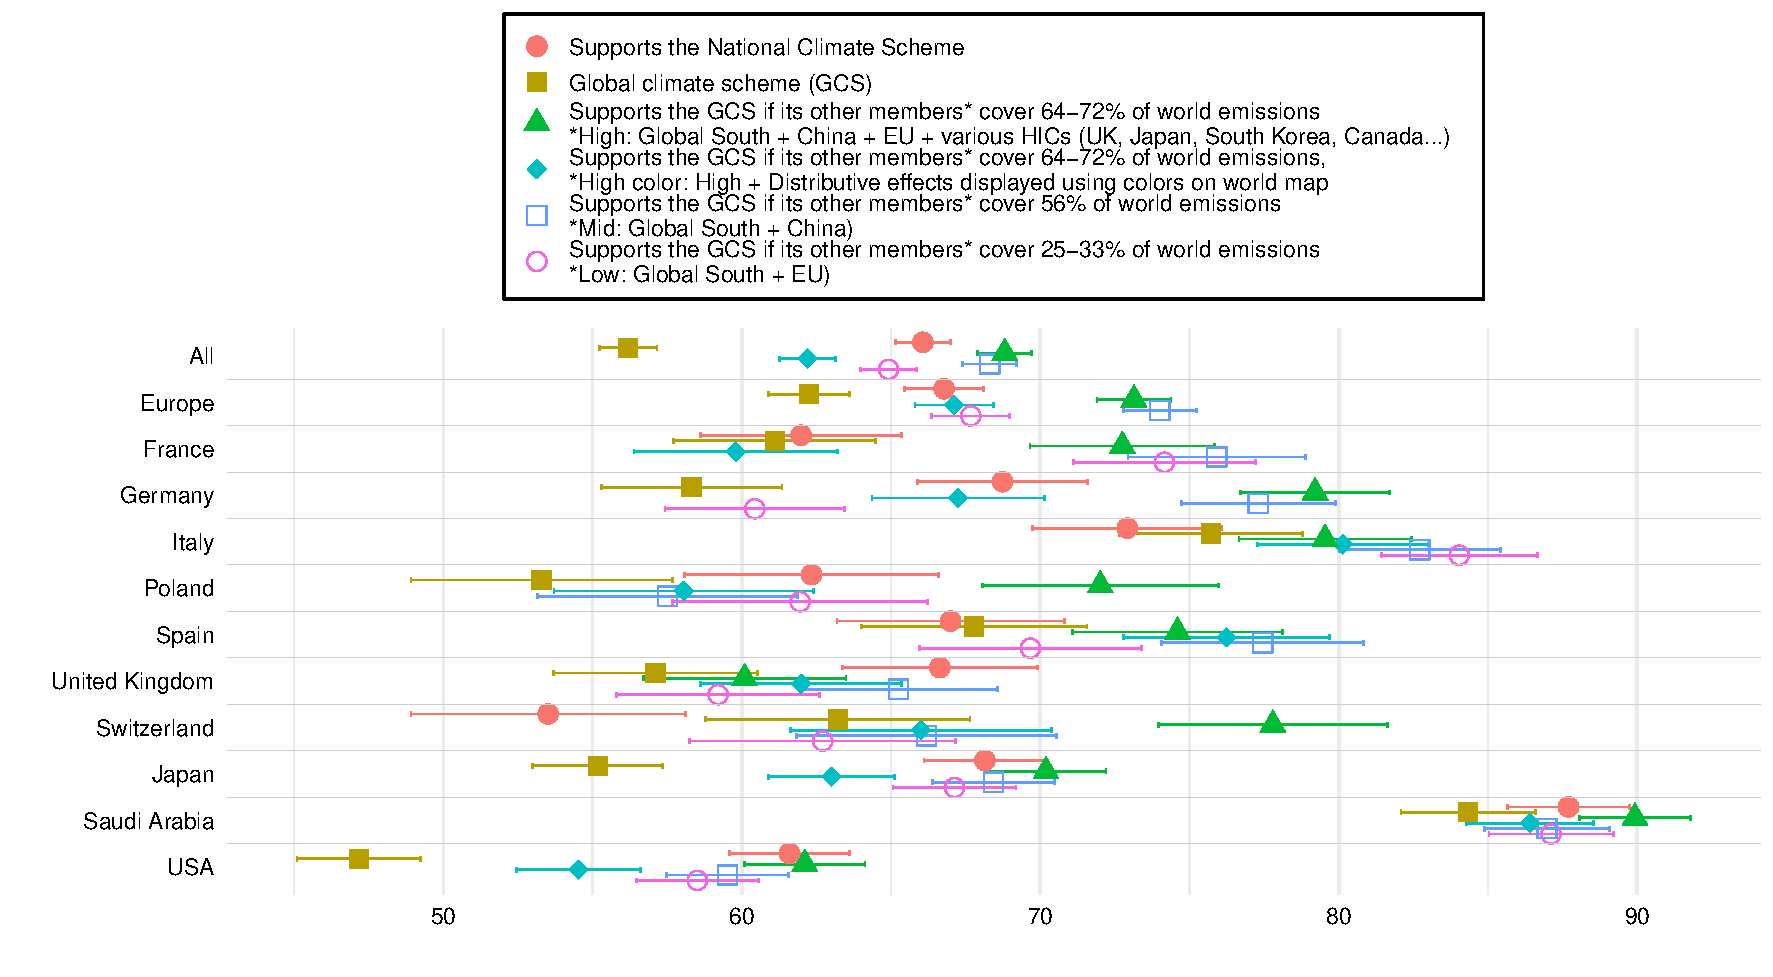
\includegraphics[width=\textwidth]{../figures/country_comparison/variables_ncs_gcs_ics_by_country}
\begin{figure}[h!]
    \caption[Support for the NCS, GCS, ICS]{Support for the National, Global, and International Climate Schemes (\textit{Yes}/\textit{No} question). \hfill (Questions \ref{q:ncs_support}-\ref{q:ics_support}).
    }\label{fig:ics}
    \makebox[\textwidth][c]{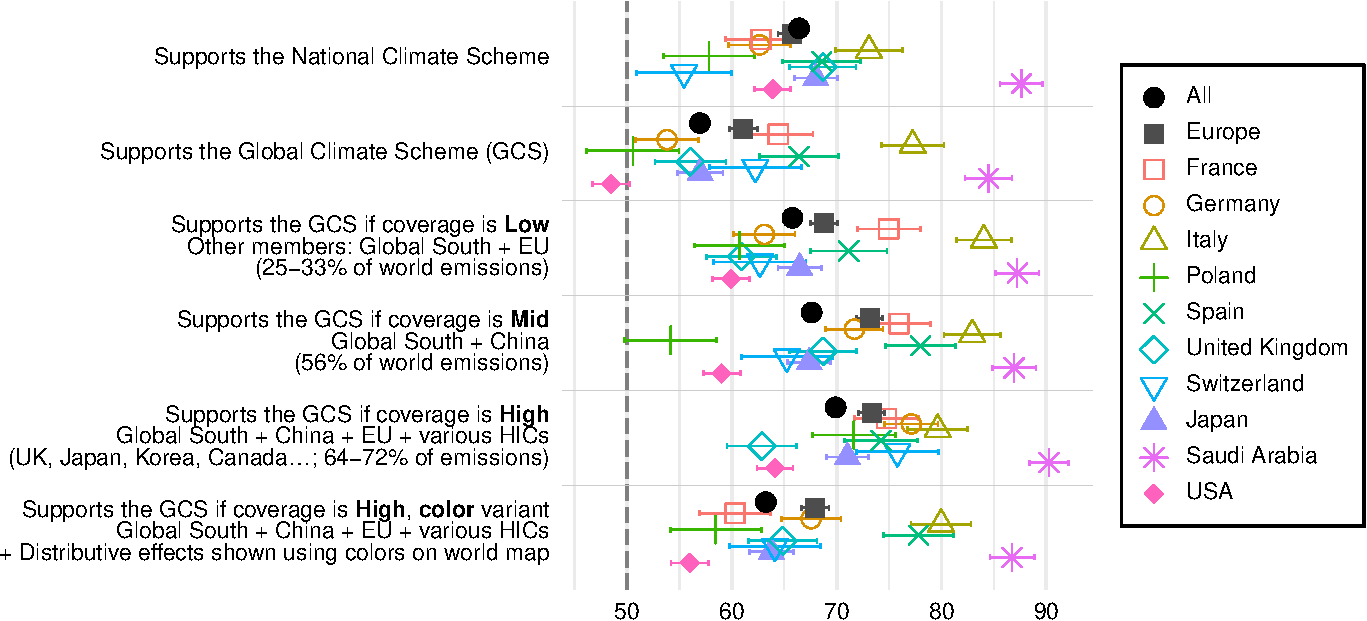
\includegraphics[width=\textwidth]{../figures/country_comparison/variables_ncs_gcs_ics_control_by_country.pdf}} 
\end{figure}

As expected, the wider the coverage, the higher the support. However, this effect is relatively small, as the support is only 4~p.p. higher in the \textit{High} compared to the \textit{Low} variant. Interestingly, among Europeans, the support significantly increases when China is added to coalition, but not significantly more when other HICs are also added. Conversely, for US-Americans and Japanese, the participation of the EU or China yield similar levels of support, and only the combined participation of China, the EU, and other HICs significantly increase the support. 

The support is 6.5~p.p. lower in the \textit{High color} compared to the \textit{High} variant. Three reasons may explain this effect. First, some respondents may be concerned by the information (made explicit in the question) that China would neither gain nor lose from the policy. 
Second, with the colored map, respondents learn how their own country fares compared to other countries. Actually, the effect is 1~p.p. and no longer significant for countries that appear to lose less than 0.5\% of their GDP (Spain and Switzerland). Third, the cost may be more salient with the colored map. Interestingly, the support for the GCS is 5~p.p. lower for the 74\% of respondents who understand that it would result in increased gasoline prices (after controlling for sociodemographics), but this effect is only 2~p.p. and no longer significant for the \textit{High color} ICS, indicating that the information provided by the map mostly affects those who had not yet understood the policy's consequences. 

Notice that the support for the ICS's \textit{Low} coverage is similar to that for the NCS. This suggests that the average respondent is willing to pay the ICS's higher cost for the guarantee of poverty alleviation and decarbonization in the Global South. %This suggests that, for the average person, the guarantee of poverty alleviation and decarbonization in the Global South balances out the ICS's higher cost. 
Finally, the greater support for the ICS compared to the GCS is somewhat puzzling. Perhaps, people view the proposal as more credible when a list of countries is provided, compared to the GCS that is framed as if all countries might join (or on the contrary, in which the participation of any country is uncertain). Relatedly, support may be stronger for more precise or more visual proposals, either because they are viewed as more advanced or because they induce an experimenter demand bias. The greater support could also be due to costs being less salient in the ICS question (but the support is still greater than in the GCS in the \textit{High color} variant, where costs are visible). Unfortunately, the data does not allow testing these different hypotheses.

% support increases with coverage
% ICS low: similar to NCS: people willing to pay Global South for its decarbonization
% ICS mid, high: higher acceptance: people happier with less free-riding
% ICS high color: visualizing net gain stronger effect than country coverage
% why GCS < ICS? hypotheses: lower support for less concrete / more uncertain proposal, cost less salient, map induces more experimenter demand, people think it's more credible if it's about joining a club (rather than a GLOBAL cs), stronger effect of not-wanting-to-free-ride when see most countries are in

\subsection{Wealth tax funding LICs}\label{subsec:wealth_tax}

I test the effect of country coverage on the support for an internationally redistributive wealth tax using a simple \textit{Yes}/\textit{No} question with three random variants. The policy is described as a 2\% tax on wealth above \$1~million, with 30\% of its revenue financing public services in LICs. In the \textit{Global} variant, all other countries (i.e. all countries except the respondent's one) are assumed to participate. The \textit{HIC} variant covers all other HICs. The \textit{International} variant covers some countries and not others, with the precise coverage varying by respondent's country but always including Brazil and European countries (or the whole EU) and excluding China and the U.S.\footnote{More precisely, in the U.S., excluded countries differ and are China, Japan, and Canada. As for included countries, on top of Brazil, they are: the EU and the UK for Switzerland, Saudi Arabia, and the U.S.; the EU for Russia and the UK; and France, Germany, Spain, and the UK (except one's own country) for EU countries.}

Here again, the support increases with the country coverage, but the effect is small. The middle-ground \textit{HIC} variant garners 70\% support (from 58\% in Switzerland to 81\% in Saudi Arabia). Compared to \textit{HIC}, the support is 5~p.p. higher in the \textit{Global} coverage, while it is only 1.5~p.p. and non-significantly lower in the \textit{International} coverage (Figure \ref{fig:wealth_tax}). 

% # 5b. wealth tax by coverage: 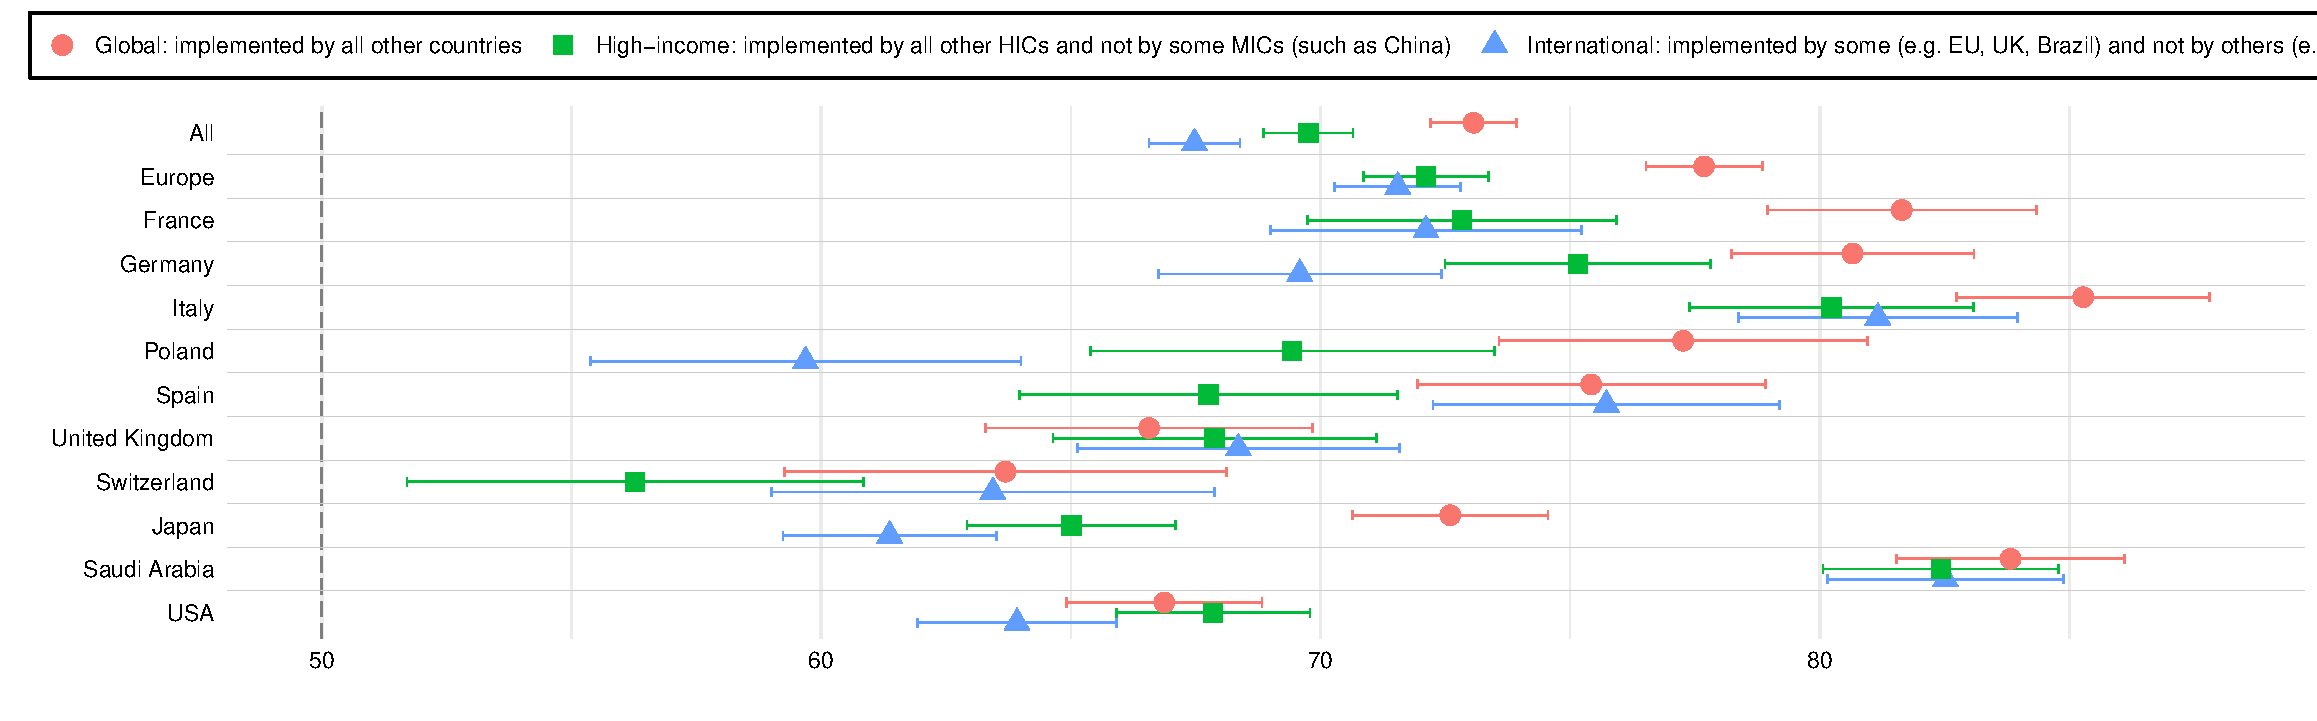
\includegraphics[width=\textwidth]{../figures/country_comparison/variables_wealth_tax_support_by_country}
\begin{figure}[h!]
    \caption[Support for an international wealth tax depending on country coverage]{Support for an international wealth tax with 30\% of revenue funding LICs, depending on the country coverage (\textit{Yes}/\textit{No} question). \hfill (Questions \ref{q:global_tax_support}-\ref{q:intl_tax_support}).
    }\label{fig:wealth_tax}
    \makebox[\textwidth][c]{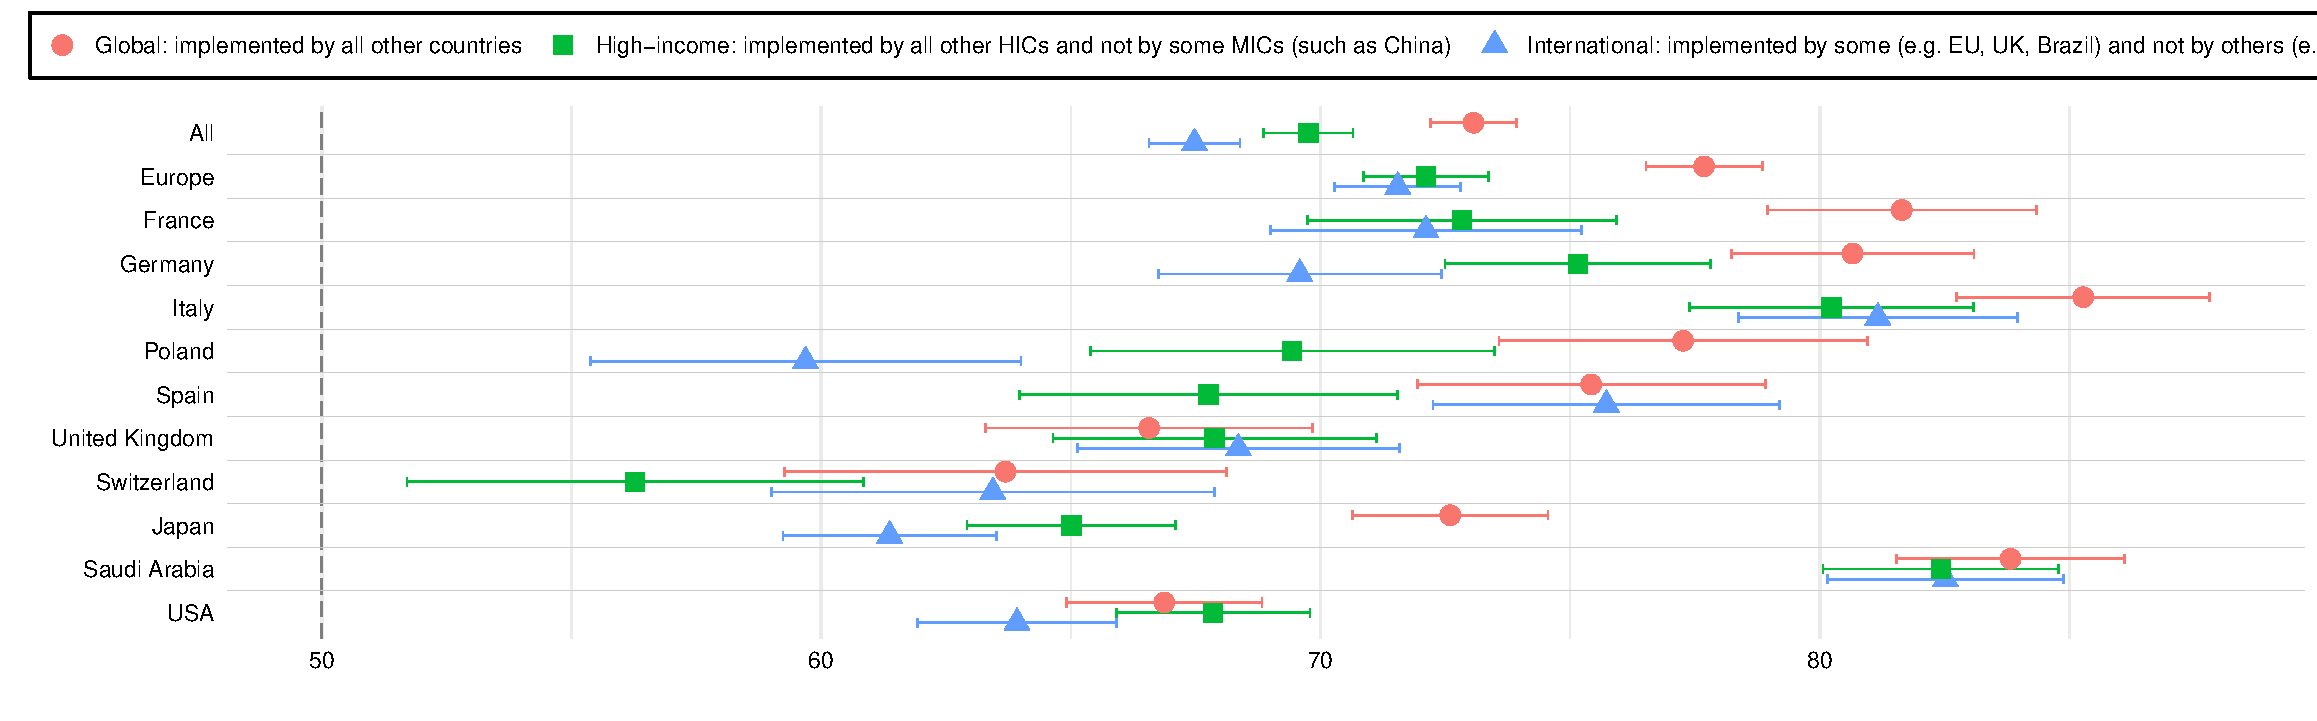
\includegraphics[width=.9\textwidth]{../figures/country_comparison/variables_wealth_tax_support_by_country.pdf}} 
\end{figure}

Overall, the results indicate that the support for internationally redistributive policies is quite robust to country coverage. This suggests that the issues of competitiveness or free-riding issues are not decisive in public support. % TODO? cite Bernauer & Gampfer, Aklin & Mildenberger

\section{Sincerity of support for global redistribution\label{sec:sincerity}}

Skeptics about the public's support for global redistribution would argue that the support is not reflected in real-stake decisions and that it mostly results from \textit{warm glow}. According to the \textit{warm glow} hypothesis, many people would express their support to enjoy moral comfort as long as public support seems harmless since the policy appears out of reach, but support would vanish if (\textit{i}) the prospect of implementation materialized or if (\textit{ii}) moral comfort could be obtained from a substitute. In this Section, I test whether global redistribution is a vote-determining issue using a conjoint analysis, and I test both forms of \textit{warm glow} (\textit{i} and \textit{ii}) using two other survey experiments.
% - No (or little) evidence of warm glow or support due to unrealism; global redistr genuinely supported (conjoint analysis)

\subsection{Conjoint analysis}\label{subsec:conjoint}

I run a conjoint experiment in all countries except Russia and Saudi Arabia. This question is positioned at the beginning of the survey, before respondents can know the survey's topic. Respondents are presented with two random political programs, framed as the fictive programs of the top candidates in the next election, and asked which of the candidate they would vote for (27\% of the respondents choose the outside option \textit{Neither of them}). Each program contains a policy or an absence of policy chosen at random for each of five policy domains (the order of which is also randomized). %: \textit{Economic issues}, \textit{Social issues}, \textit{Climate policy}, \textit{Tax system}, \textit{Foreign policy}. 
Our domain of interest is \textit{Foreign policy}, whose pool contains three policies: \textit{Cut development aid}, \textit{International tax on millionaires with 30\% financing healthcare and education in low-income countries}, and a country-specific policy. % (e.g. \textit{Support Ukraine militarily and financially} in Germany). 
I included both a \textit{pro}- and an \textit{anti}-global redistribution policy to capture a potential status quo bias, or on the contrary, a bias in favor of (any) reform. 
Except for these two policies of interest, the policies have been selected from the programs of the main candidates in the country's last election, so as to span the entire political spectrum and cover the most prominent proposals in the country's public debate. 

Figure \ref{fig:conjoint} shows the effect of our policies of interest's presence in a program on the likelihood that it is preferred (see Figures \ref{fig:conjoint_FR}-\ref{fig:conjoint_ES_original} for full results country-by-country\footnote{With some exceptions, raising the minimum wage is among the most popular policies, together with redistributive taxes or transfers, anti-immigration regulations, and abortion rights. % TODO: study party of most/least popular policies by country
Conversely, a ban on new combustion-engine cars is among the least popular ones.}). 
% TODO! cluster standard errors by respondent
% TODO! why Japan millionaire significant in conjoint_JP but not in conjoint?
More specifically, Figure \ref{fig:conjoint} presents the results %estimates of coefficients $\beta_1$ and $\beta_2$ 
of the following regression estimated by simple OLS, with standard errors clustered by respondent: 
$$\text{Preferred}_{pi} = \beta_1 \text{Cut\_aid}_{pi} + \beta_2 \text{Intl\_tax}_{pi} + \beta_3 \text{Foreign3}_{pi} + \varepsilon_{pi}$$
where $pi$ denotes either program $p$ faced by respondent $i$, and each variable is a dummy. 

% # 6. conjoint: foreign aid + global tax (per country + global)
\begin{figure}[h!]
\caption[Conjoint analysis: effect of development aid and millionaire tax]{Effect on the likelihood that a political program is preferred of containing the following policy (compared to no foreign policy in the program). (See Figure \ref{fig:conjoint_vote} for effects by vote). \hfill (Question \ref{q:conjoint})} \label{fig:conjoint}
\begin{subfigure}{.49\textwidth}
  \caption[]{Cut development aid}
  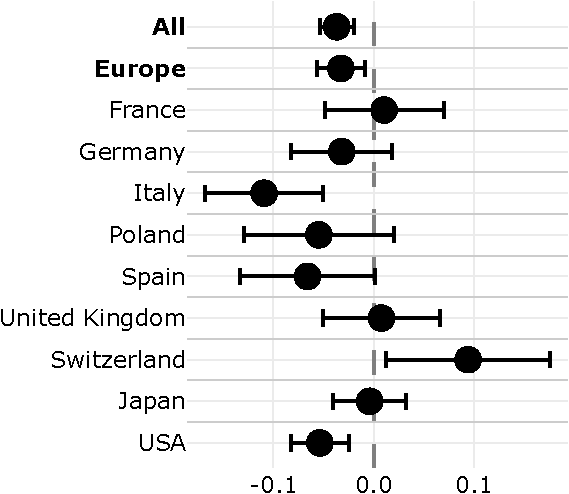
\includegraphics[height=.36\textheight]{../figures/country_comparison/program_preferred_by_cut_aid_in_program.pdf}
\end{subfigure} 
\begin{subfigure}{.49\textwidth}
  \caption[]{International tax on millionaires with 30\% financing health and education in low-income countries}%\begin{flushright}
  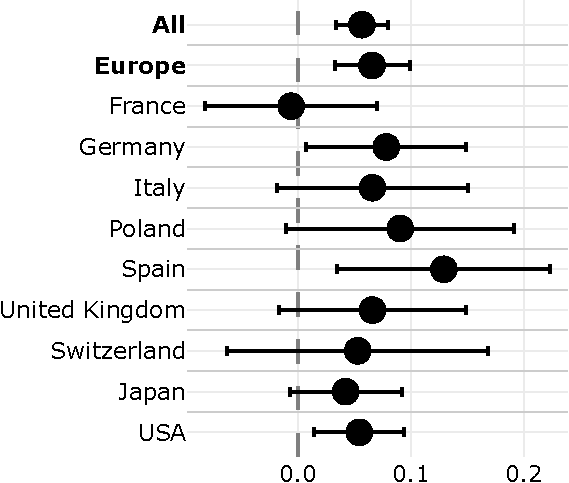
\includegraphics[height=.36\textheight]{../figures/country_comparison/program_preferred_by_millionaire_tax_in_program.pdf}%\end{flushright}
\end{subfigure}
\end{figure}

Both policies significantly affects the program choice: the internationally redistributive millionaire tax increases by 4~p.p. the likelihood that a program is preferred, while cutting development aid decreases it by 4~p.p. On a single country, the effects are generally non-significant due to lack of power, but when significant, they are of the same sign as the global effect, except for \textit{Cut aid} in Switzerland. Overall, the effects are of comparable size to the effects of other policies, % TODO justify
suggesting that global redistribution issues may be as vote-determining as policies prominent in the national debate. 

One concern with this type of conjoint analysis is that they involve unrealistic political programs, namely programs that contain both left and far right policies, which distorts the real choice that voters may face. \cite{cuesta_improving_2022} showed that to fully address this issue, one should weigh each pair of programs by the probability that such a pair would be proposed in a real election. As such probability cannot be computed, the best practice is to bound the effects by estimating them with extreme probabilities. The results just presented are based one extreme, the uniform distribution. To construct the other extreme, I classify each policy as left, center, or right, and assume that a program is consistent if it does not contain policies from both the left and the right. I then re-estimate the regression after dropping all pairs an inconsistant program (effectively assigning a probability of zero to them). I first classify our policies of interest as \textit{center} (considering them as consistent with any program), in which case 59\% of observations are retained, and effects are preserved. This indicates that our results are robust to the critique of \cite{cuesta_improving_2022}. Interestingly, the effects differ when I classify our policies of interest as \textit{left} (for the tax) and \textit{right} (for cutting aid), in which case only 39\% of observations are retained. In that case, the effect of the millionaire tax is preserved, but the effect of cutting aid vanishes to 0~p.p. In other words, the effect of cutting aid disappears when removing left-leaning programs where it is present, while the effect of the tax remains the same when removing right-leaning programs where it is present. Therefore, cutting aid is harmful only for left-leaning programs, while a wealth tax is helpful for any program. Interestingly, this does \textit{not} mean that only left-wing voters oppose cutting aid while an international wealth tax would be vote-determining for right-wing voters. %(as non-voters or right-wing voters may be tempted by left-wing programs and vice versa). TODO? put back?
Indeed, the results by vote show that the tax has a negative (though non-significant) effect among right and far right voters, while cutting aid has a significant effect of $-$2.5~p.p. on \textit{Center-right or Right} voters (Figure \ref{fig:conjoint_vote}), 


\subsection{Testing warm glow}\label{subsec:warm_glow}

Some people might claim they support a policy of global redistribution just to ease their conscience. If support were mainly due to such a psychological mechanism, called \textit{warm glow}, it might
dissipate when the prospect of the policy materializes or if the policy can be replaced by a substitute with the same moral appeal.

\paragraph{Moral substitute.}

Following \cite{nunes_identifying_2003}, warm glow would be revealed if support for the GCS were reduced after respondents are offered the possibility to express generosity towards the cause of climate change. To test this hypothesis, right before the GCS page, I assign a random subset of the respondents to a donation lottery, while the control group faces no question.\footnote{More precisely, right before the GCS question, the sample is split into three branches: the \textit{Donation} lottery, the \textit{NCS} question, and the control group. The NCS treatment is excluded from this analysis as it is unrelated to this experiment (it was created to prevent the NCS question from influencing answers on the GCS).} 
In the \textit{Donation} branch, respondents have to decide how much they would donate to the reforestation NGO \textit{Just One Tree}, should they win the question's \$100 lottery. 
A lower support of the GCS in the treated group would be evidence of warm glow, as it would indicate that the support (at least partially) derives from a moral satisfaction at having recently supported a just cause. 

% # 7. warm_glow: effect of info + display donation vs. control (per country + global)
    \begin{figure}[h!]
\caption[Testing warm glow]{Testing warm glow (negative effects would indicate the presence of warm glow).}\label{fig:warm_glow}
\begin{subfigure}{.45\textwidth}
  \caption[]{Effect of a \textit{Donation lottery} treatment on support for the Global Climate Scheme. (Questions \ref{q:donation}-\ref{q:gcs_support})\label{fig:warm_glow_substitute}}
  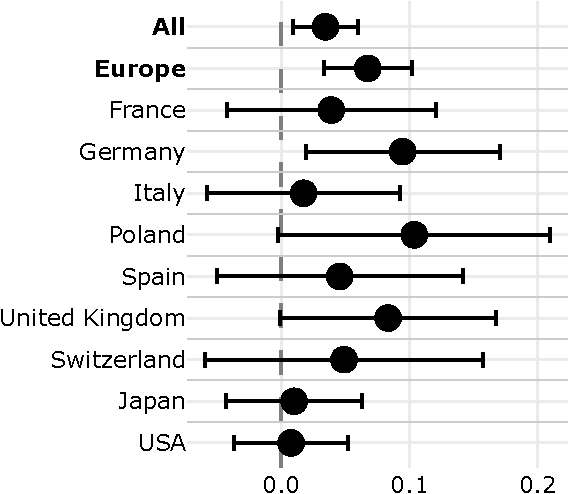
\includegraphics[height=.36\textheight]{../figures/country_comparison/gcs_support_by_variant_warm_glow.pdf}
\end{subfigure} \quad
\begin{subfigure}{.49\textwidth}
  \caption[]{Effect of information about ongoing global redistribution initiatives on the share of plausible global policies supported. (Questions \ref{q:info_solidarity}-\ref{q:solidarity_support})\label{fig:warm_glow_realism}}
  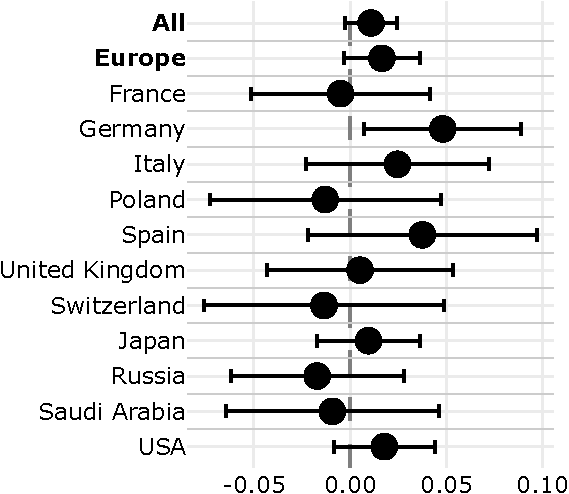
\includegraphics[height=.36\textheight]{../figures/country_comparison/share_solidarity_supported_by_info_solidarity.pdf}
\end{subfigure}
\end{figure}

On the contrary, support for the GCS is 3.5~p.p. higher in the \textit{Donation} branch compared to the control group, and the coefficient is positive in every country, though often not significant (Figure \ref{fig:warm_glow_substitute}). While it remains unclear why the effect is positive,\footnote{Perhaps the \textit{Donation} question triggers thoughts favorable to the GCS, such as the realization that individual actions like donations are ill-suited to address climate change so that we need a global policy, even if imperfect.} 
the results show no evidence of warm glow.

\paragraph{Realism treatment.}

To test whether some people express support for global redistribution only for as long as its implementation seems unlikely, I randomly treat half of respondents with information about ongoing negotiations on globally redistributive policies. Among other things, treated respondents are informed that the International Maritime Organization recently adopted a levy on maritime carbon emissions that should partly finance LICs; that the G20 considered the introduction of a global tax on billionaires; that the UN General Assembly recently agreed on the principle of expanding the UN Security Council to new members; and that the UN Secretary General supports reforms to the financial system that would drive resources towards sustainable development. 
Then, respondents are asked ``how likely [it is] that international policies involving significant transfers from HICs to LICs will be introduced in the next 15 years'', right before testing their support for ten plausible global policies, described in Section \ref{subsec:debated}. Here, warm glow would be revealed if the information treatment increased the belief that global redistribution is likely but decreased the support for global policies. %(as respondents would fear that such policies may materialize).

Informed respondents are 8~p.p. more likely to believe that global redistribution is likely (with only 35\% believing so in the control group, cf. Table \ref{tab:iv}). With an F-Statistic of 72, this highly significant effect makes for a strong first stage in an instrumental variable (IV) strategy to estimate the effect of believing that global redistribution is likely on the share of global policies supported. As shown in Table \ref{tab:iv}, the Local Average Treatment Effect estimated by IV is 15~p.p., indicating that believing that global redistribution is likely causally \textit{increases} the share policies supported. This effect is consistent with the non-causal effect estimated by OLS at 15~p.p., and with the direct effect of the treatment on the share of policies supported, estimated at 1~p.p. with a \textit{p}-value of 0.06 (Figure \ref{fig:warm_glow_realism}). % TODO wording p-value

% # 7bis: 2SLS 
\begin{table}[!htbp] 
  \caption[Effect on support for global redistribution of believing that it is likely]{Effect on support for global redistribution of believing that it is likely.}\label{tab:iv} 
  \makebox[\textwidth][c]{
% Table created by stargazer v.5.2.3 by Marek Hlavac, Social Policy Institute. E-mail: marek.hlavac at gmail.com
% Date and time: lun., oct. 20, 2025 - 18:22:12
\begin{tabular}{@{\extracolsep{5pt}}lcccc} 
\\[-1.8ex]\hline 
\hline \\[-1.8ex] 
\\[-1.8ex] & \makecell{Believes global\\redistr. likely} & \multicolumn{3}{c}{Share of plausible global policies supported} \\ 
 & IV 1st Stage & IV 2nd Stage & OLS & Direct Effect \\ 
\\[-1.8ex] & (1) & (2) & (3) & (4)\\ 
\hline \\[-1.8ex] 
 Information treatment & 0.078$^{***}$ &  &  & 0.011$^{*}$ \\ 
  & (0.009) &  &  & (0.006) \\ 
  Believes global redistribution likely &  & 0.139$^{*}$ & 0.150$^{***}$ &  \\ 
  &  & (0.080) & (0.006) &  \\ 
  (Intercept) & 0.331$^{***}$ & 0.457$^{***}$ & 0.453$^{***}$ & 0.503$^{***}$ \\ 
  & (0.006) & (0.030) & (0.004) & (0.004) \\ 
 \hline \\[-1.8ex] 
Effective F-statistic & 65.61 &  &  &  \\ 
Observations & 12,007 & 12,007 & 12,007 & 12,007 \\ 
R$^{2}$ & 0.006 & 0.043 & 0.043 & 0.0002 \\ 
\hline 
\hline \\[-1.8ex] 
\textit{Note:}  & \multicolumn{4}{r}{$^{*}$p$<$0.1; $^{**}$p$<$0.05; $^{***}$p$<$0.01} \\ 
\end{tabular} 
}
\end{table}

Again, the effects go in the opposition direction to warm glow. In this case, increased support may stem from enhanced credibility of policies that are known to be discussed in international organizations. 
Overall, the results of these two experiments provide no evidence that support for global redistribution is affected by warm glow. On the contrary, they suggest that support is sincere and robust to the prospect of implementation or to the possibility of a moral substitute.


\section{Breadth of international policies accepted\label{sec:breadth}}

Knowing that some internationally redistributive policies are sincerely supported and may be vote-determining, I now study the breadth of international policies that may be accepted. In this Section, I analyze in turn the support for global policies currently debated in the international community, for more radical proposals, broader willingness to defend global solidarity, the preferred channels to transfer resources to LICs, and a custom redistribution task that aims to reveal the preferred extent of international transfers. 
% - People ready to sustainability and radical global redistr (for duty, not reparations)
% - People favor social protection to unconditional transfers

\subsection{Support for currently debated global policies}\label{subsec:debated}

\paragraph{Plausible global policies.}

Figure \ref{fig:solidarity_support_share} reveals the relative support for plausible global policies, % TODO: links to these proposals/negotiations
% TODO! RU security council
i.e. the share of \textit{Somewhat} or \textit{Strong support} among non-\textit{Indifferent} answers. Almost each policy garners relative majority support in each country. The only exceptions is the support of Japanese for a globally redistributive tax on carbon emissions from aviation, at 46\%. % TODO RU profit tax?
This proposal is the one with the most salient cost, which a 30\% increase in the price of flights; it is the least support in every country except for Russia. The most supported policies, with above 70\% of relative support in every country, are the 2\% minimum tax on billionaires' wealth proposed by \cite{zucman_blueprint_2024} and the expansion of low-interest rates sustainable investments in LICs \citep{bridgetown_initiative_bridgetown_2025}. 

% # 8. solidarity_support (on control): heatmap 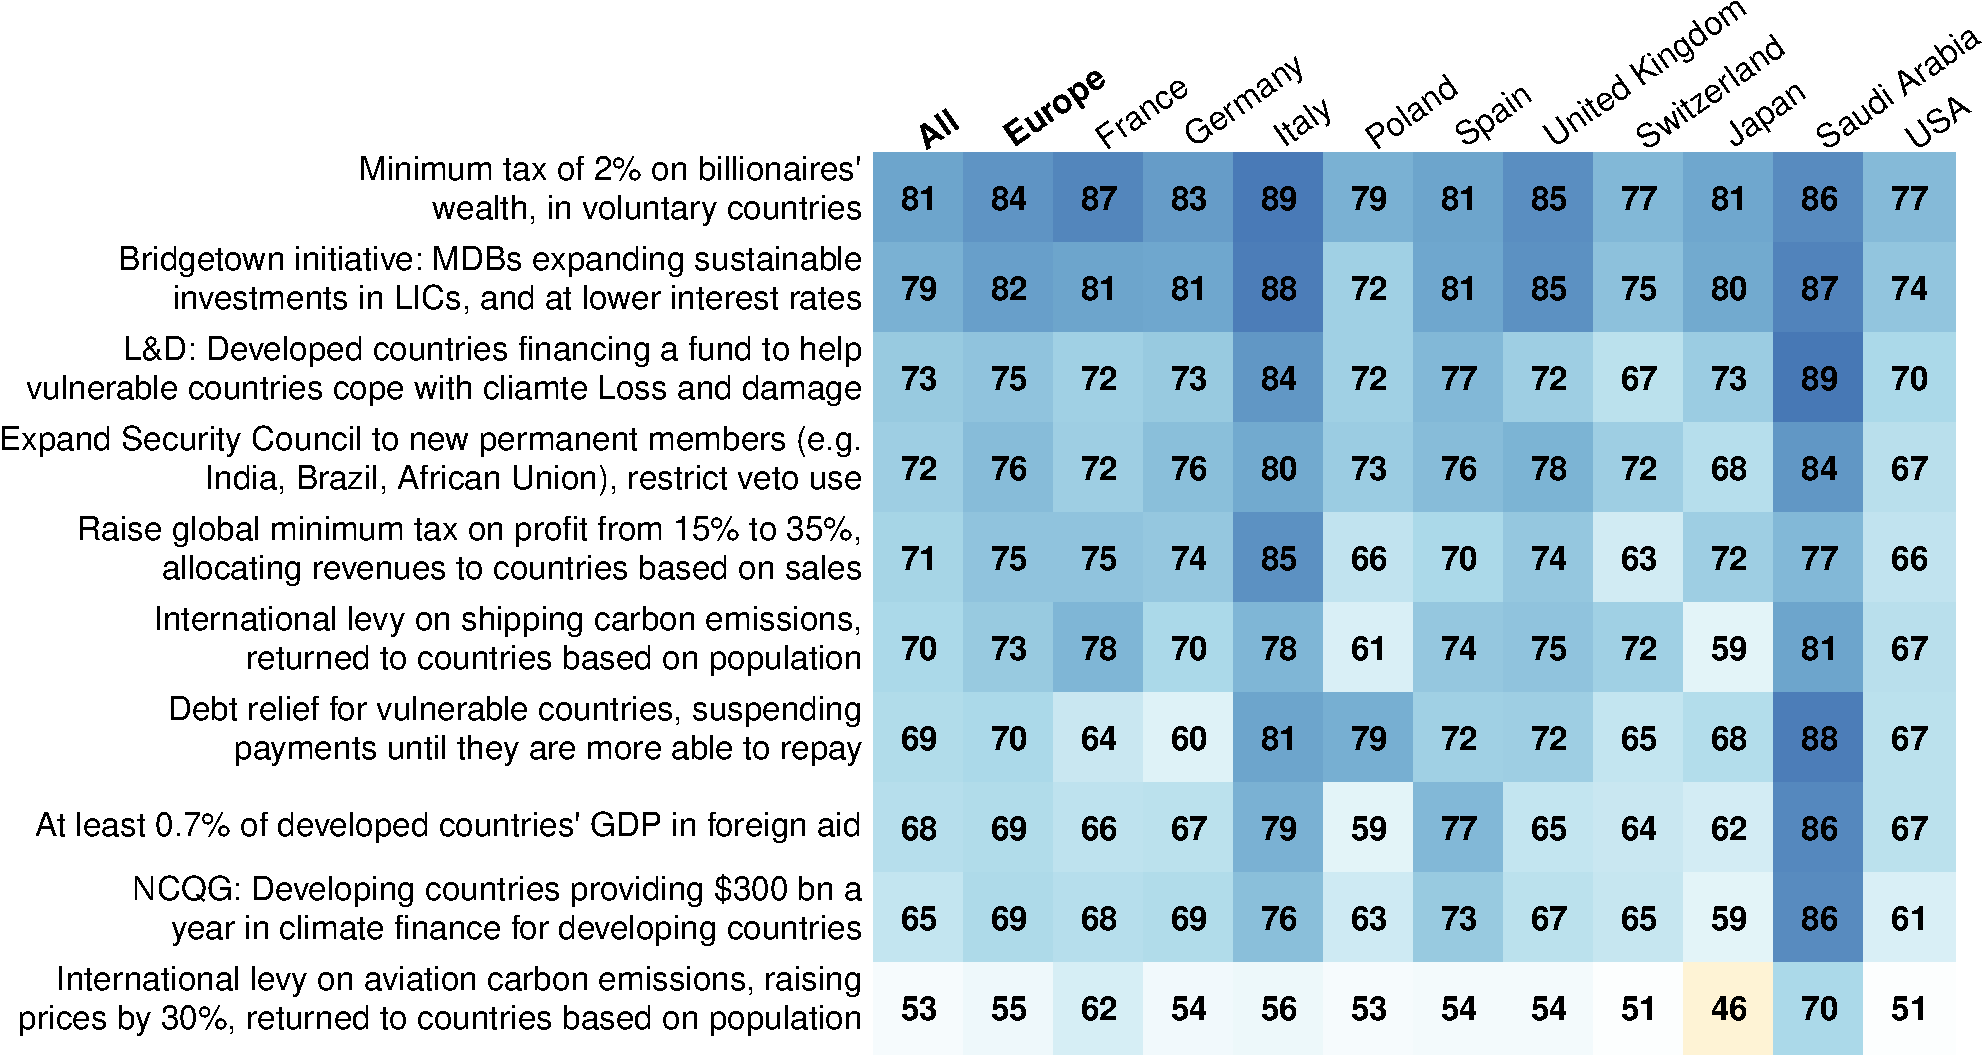
\includegraphics[height=.89\textheight]{../figures/country_comparison/solidarity_support_share}
\begin{figure}[h!]
    \caption[Relative support for plausible global redistribution policies]{Relative support for plausible global redistribution policies (Percentage of \textit{Somewhat} or \textit{Strongly support} among non-\textit{Indifferent} responses). (Question \ref{q:solidarity_support}).
    }\label{fig:solidarity_support_share}
    \makebox[\textwidth][c]{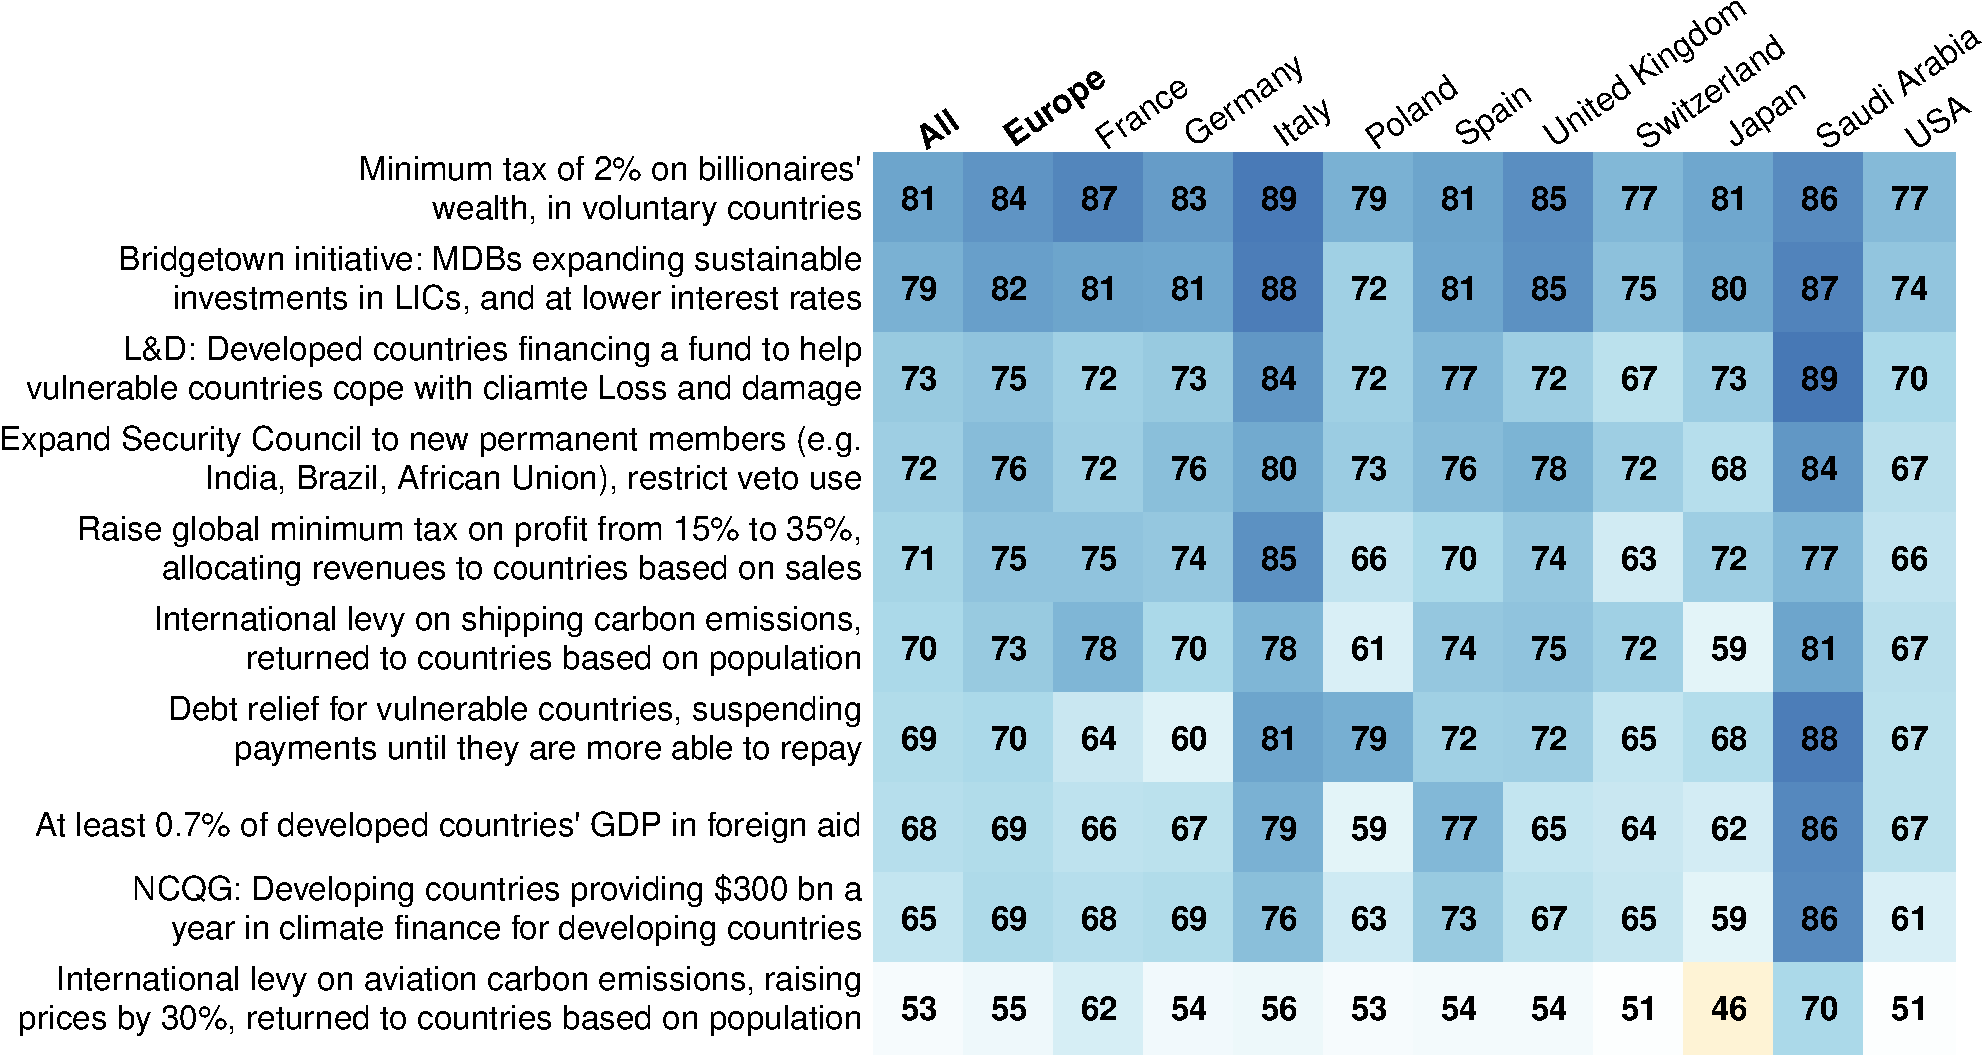
\includegraphics[width=\textwidth]{../figures/country_comparison/solidarity_support_share.pdf}} 
\end{figure}

% The share of plausible policies supported ranges from 38\% in Japan to 66\% in Saudia Arabia and 65\% in Italy. Conversely, the share of policies opposed is highest in Switzerland (29\%), Poland %(23\%) 
% and the U.S. (23\%). The other questions exhibit a similar ranking of countries. 
On average, respondents support 51\% of the plausible policies and oppose 20\% of them, meaning that they support +31~p.p. more policies than they oppose. The most supportive countries, in terms of this average mean difference between support and opposition, are Saudia Arabia (+50~p.p.), Italy (+49) and Spain (+39) while the least supportive are Japan (+20), Switzerland (+24), Poland and the U.S. (+25). 
We may wonder why the countries leading in support are the Saudi kingdom and right-wing-dominated Italy. Decomposing the support by political leaning and other selected sociodemographics, Figures \ref{fig:main_radical_redistr_pol} and \ref{fig:solidarity_support_pol_share} shed some light on this question. In Saudi Arabia, half of the adult population is immigrant. However, foreign workers do not drive the results, as Saudi citizens have indistinguable attitudes from non-Saudis.\footnote{Therefore, temptative explanations may rather come from the Saudi society: 
while Saudis benefit from a generous welfare State, the Islamic principle of \textit{Zakat} (almsgiving) might further foster a culture of generosity.} 
As for Italy is both the country with the lowest gap in support between left-wing and far right voters (together with Japan, at 33~p.p.), and the highest support among left-wing voters.\footnote{While the former point may be linked to the vision of Italy's far right leader of an Africa-Italy partnership (trading off foreign aid with cooperation on fighting immigration), the Italian population might also be influenced by messages in favor of global solidarity from the Vatican.} 

\paragraph{Climate finance goal.}

Climate finance is the financing of climate action from developed countries in developing countries. In 2024, countries agreed on a ``New Collective Quantified Goal'' (NCQG) of climate finance at \$300~billion per year by 2035, tripling the previous goal. However, while developing countries such as India called for \$600~billion in grants (or grant-equivalent funding), the NCQG does not specify which share should be provided as grants, and the current goal is currently met with only \$26~billion in grants \citep{oecd_climate_2024} (and the rest in loans). 

I test the preferred amount for the NCQG using two random variants. Both variants inform respondents of the current situation and agreed goal, and express amounts both in absolute terms and in proportion of developed countries' GDP. The \textit{Short} variant uses qualitative, textual answers, with a middle-point at \$100~billion (namely, ``Meet the newly agreed goal by tripling grants and loans (\$100 billion in grants, or 0.15\% of GDP).''). The \textit{Long} variant provides more detailed explanations in the question text and then uses numerical answers, with a middle-point at \$300~billion. 

In both variants, the median preferred NCQG is \$100~billion, and 19\% of respondents choose an amount of \$600~billion or larger. That differently framed variants yield consistent results suggests that the question was well understood, despite its length. 
The median choice of a climate finance quantum in line with the internationally agreed NCQG may be interpreted in two distinct ways. Either diplomats of HICs currently defend the median generosity 
%sentiment 
of their people, or respondents' attitudes are anchored in existing agreements (or in their governments' stance). The results presented below are more in line with the latter interpretation, as they reveal majority acceptance for much larger international transfers.


\subsection{Support for radical proposals, political action, and broad values}\label{subsec:radical}

In the last part of the questionnaire, I ask diverse questions to understand the range of policies, actions or values that people may accept regarding global solidarity (Figure \ref{fig:radical_redistr_share}).

\paragraph{Sustainable future vs. status quo.}

Respondents are asked which scenario they would prefer for the next twenty years: a sustainable future or the status quo (note that scenarios were not called that way in the questionnaire, and instead randomly named \textit{A} or \textit{B}). In the sustainable scenario, most countries cooperate to tax millionaires and meet the +2\textdegree{}C target, through an electrification of cars and the doubling of prices of heating fuel or gas, air travel, and beef. Although overall purchasing power is preserved (through a reduction in sales tax), people change their habits (e.g. flying and eating meat is cut by half). In the status quo, no policy is implemented, people maintain their lifestyles, and global warming reaches +3\textdegree{}C by 2100, causing more severe disasters. 

Overall, 68\% prefers the sustainable future over the status quo.

\paragraph{Global income redistribution.}

I test the support for a global tax on top incomes to finance poverty reduction in LICs, with the tax targeting either the global top~1\% or top~3\%, depending on a random assignment. While the top~1\% variant describes an additional 15\% tax on income in excess of \$120,000 per year (at Purchasing Power Parity), the top~3\% one features additional rates of 15\%, 30\%, and 45\% above \$80,000, \$120,000, and \$1~million, respectively. Each tax is calibrated to finance the poverty gap, with poverty defined using a threshold of \$250 per month in the top~1\% variant and \$400 per month in the top~3\% one. These taxes entail international transfer of 2\% and 5\% of the world GDP, respectively. % TODO fn method
Using two numerical examples, the question explains to the respondents how the tax would affect taxpayers' income. It also states the share of affected taxpayers in the world and in their country, as well as the share of their country's GDP that would be transferred. For example, in the U.S., the top~1\% tax would affect the top 8\% and transfer 3\% of GDP, while the top~3\% tax would affect the top 18\% and transfer 8\% of GDP. These figures are about half as low in Japan and Germany, and about four times lower in France and Spain. % TODO! support among affected

Overall, 56\% (resp. 50\%) of the respondents support the top~1\% (resp. top~3\%) tax, and 25\% (resp. 28\%) oppose it. There relative majority support for the policy in every case except for Switzerland for the top~3\% tax (in which 18\% case of Swiss people would be affected).

\paragraph{Global convergence.}

A simple question captures the acceptance for global solidarity: ``Should governments actively cooperate to have all countries converge in terms of GDP per capita by the end of the century?'' Overall, 61\% answer \textit{Yes} and 25\% \textit{No}, with the lowest relative agreement (i.e. excluding people not responding%choosing not to answer
) in the U.S., at 56\%.

\paragraph{Willingness to act.}

Two questions ask the respondents how they would react to a ``worldwide movement in favor of a global program to tackle climate change, implement taxes on millionaires and fund poverty reduction in [LICs]''. 

In a multiple choice question (that was censored in Russia), 52\% of the respondents state that they ``could sign a petition and spread ideas'' for the movement (Figure \ref{fig:global_movement}) and 29\% state they could be involved the movement by either attending a demonstration (19\%), going on strike (7\%) or donating \$100 to a strike fund (10\%). Taken at face value, these results would mean that a successful global solidarity movement could collect up to \$10~billion and gather demonstrations among the largest in history, matching Earth Day mobilizations.\footnote{On April 22, 1970, 20 million US-Americans (10\% of the population) demonstrated for the environment. Since then, Earth Day events regularly mobilize hundreds of million people worldwide.} 

Asked whether they would be more or less likely to vote for the political party they feel closest to if it were part of such a movement, 36\% of the respondents state they would be more likely \textit{versus} 17\% less likely (Figure \ref{fig:vote_intl_coalition}). Among the 5\% of respondents who did not vote in the last election and feel closest to a left-wing party, the share more likely to vote in that case increases to 46\% (\textit{versus} 10\% who are less likely). 

% TODO 580 millionaires

\paragraph{Reasons for helping LICs.}

In a multiple choice question, I ask respondents which reasons for HICs supporting LICs they agree with, among arguments involving \textit{duty}, \textit{long-term interest}, or \textit{historical responsibility}. With 54\%, the reason most chosen in every country (except for France) is \textit{duty}, namely ``Helping countries in need is the right thing to do'' (Figure \ref{fig:why_hic_help_lic}). Besides, 38\% select \textit{interest} and 24\% \textit{responsibility}, with only 17\% disagreeing with every reason.

\paragraph{Reparations.}

In former colonial or slave States,\footnote{I did not ask this question in Japan or Russia, because these countries' historiography do not present their past as colonial but as a larger ``empire''.} 
I ask respondents whether they would support ``reparations for colonization and slavery to former colonies and descendants of slaves'', specifying the reparations ``could take the form of funding education and facilitating technology transfers''. Consistently with the general disagreement that HICs have a \textit{historical} responsibility to support LICs, only a minority of 35\% of respondents support reparations (except in Italy where 56\% do), while 42\% oppose them. This suggests that framing global solidarity as a decolonial struggle might be counterproductive.

\paragraph{Agreement that own taxes should solve global problems.}

% To crosscheck the findings and analyze the extent to which they could be affected by time, framing, or sampling, I reproduced a question asked in a previous study, the ``Global Solidarity Report'' \citep{global_nation_global_2023}. 
Overall, 41\% agree and 28\% disagree that ``[Their] taxes should go towards solving global problem''. With 59\% relative agreement, there is a relative majority in favor of one's own taxes financing global solidarity, though a lower one than for specific proposals that would make the richest contribute.\footnote{This confirms that the willingness to pay for global solidarity, even through taxes, does not equate to support for global redistribution proposals. %Mmeasure the same disposition as the support for global redistribution proposals. 
} 
As explained in Section \ref{sec:data} and shown in Appendix \ref{app:comparison}, the present results replicate well the ``Global Solidarity Report'' that first asked this question \citep{global_nation_global_2023}

% \paragraph{Comparison with existing surveys}

% To crosscheck the findings and analyze the extent to which they could be affected by time, framing, or sampling, I reproduced a question asked in a previous study, the ``Global Solidarity Report'' \citep{global_nation_global_2023}. Overall, 41\% agree and 28\% disagree that ``[Their] taxes should go towards solving global problem''. 
% The results replicate well the earlier study, as relative agreement, at 59\%, is just 3~p.p. higher in the present survey, and the cross-country correlation is .70 (see Figure \ref{fig:comparison} in Appendix \ref{app:comparison}). 

% Furthermore, although the question on the billionaire tax is not worded exactly as in \cite{cappelen_majority_2025}, the results are also very consistent, with an overall absolute support 4~p.p. lower in the present survey and a cross-country correlation of .86.

% # 9. radical_redistr: heatmap sustainability, top_tax, reparations, NCQG? TODO!, vote_intl_coalition, group_defended?, my_tax_global_nation, convergence_support # my_tax_global_nation other source? No, just mention corrs and means in appendix/footnote & say no sufficient confidence in their representativeness + compare w Stostad 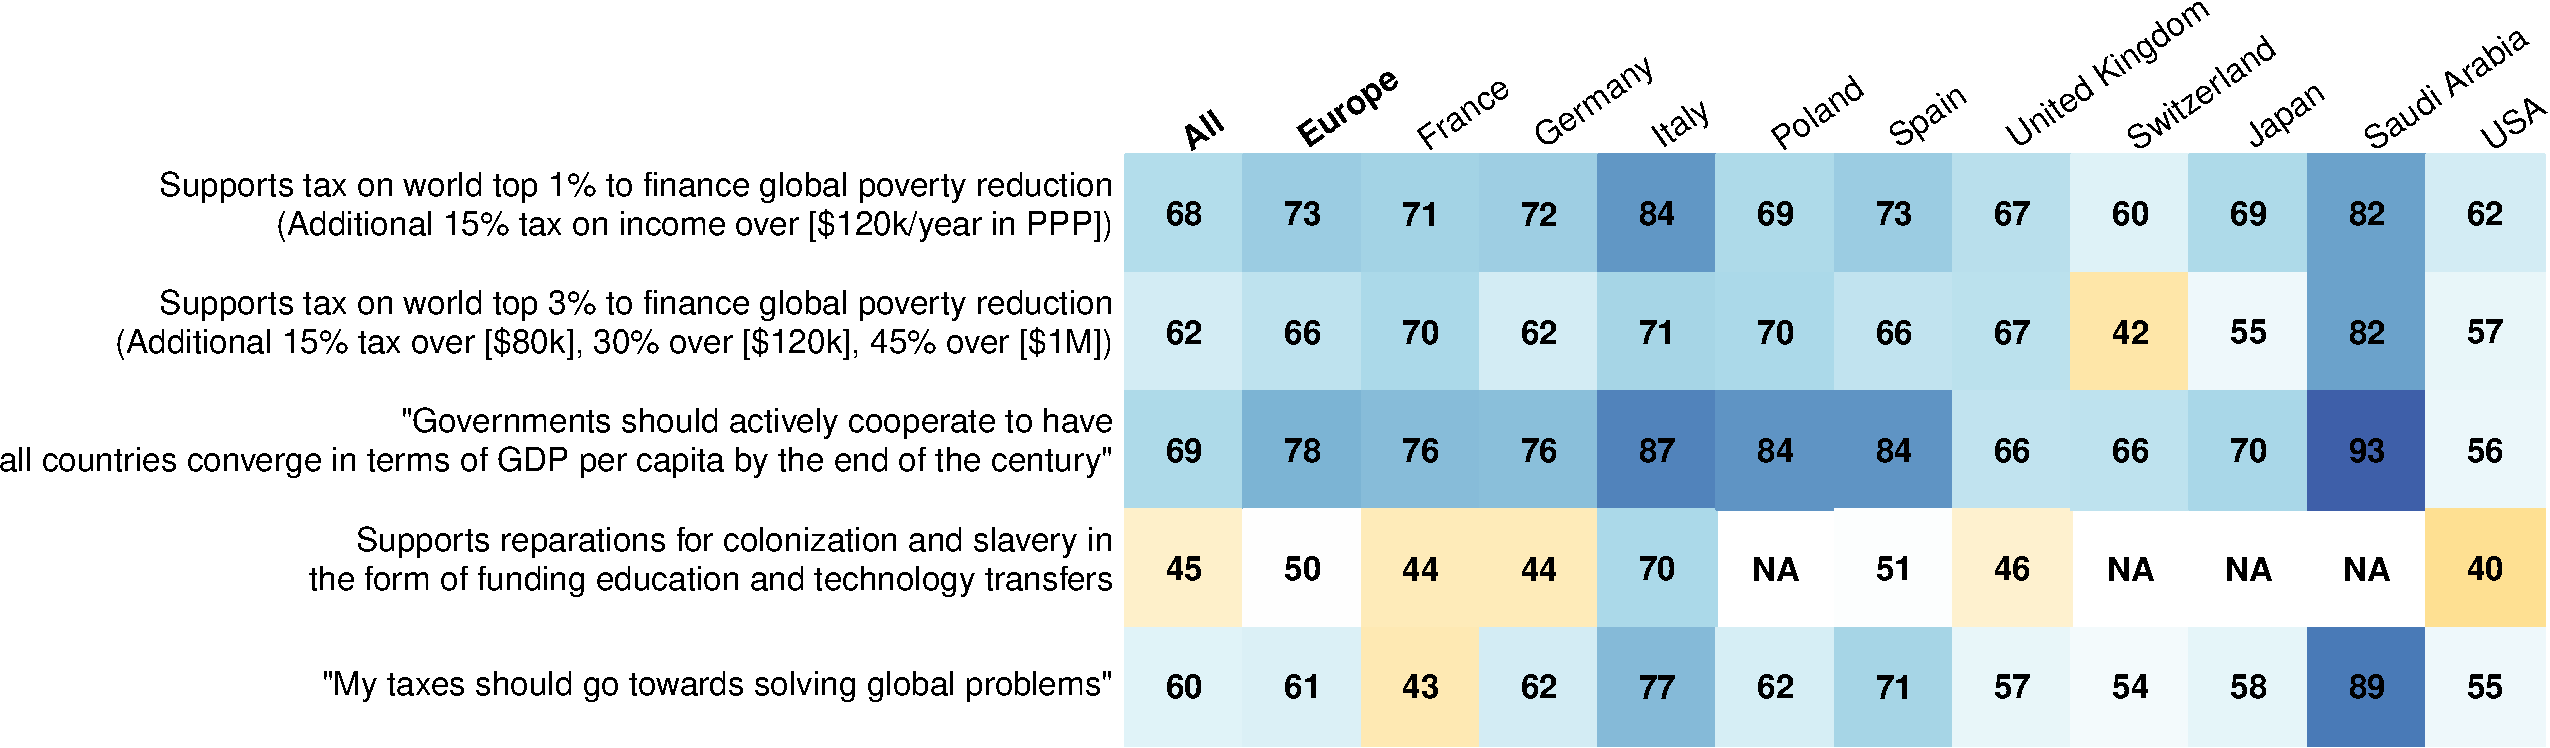
\includegraphics[width=\textwidth]{../figures/country_comparison/radical_redistr_few_share}
\begin{figure}[h!]
    \caption[Support for broad or radical global redistribution]{Support for broad action or radical proposals of global redistribution. \hfill (Questions \ref{q:sustainable_future}-\ref{q:top3_tax_support}, \ref{q:convergence_support}-\ref{q:vote_intl_coalition}, \ref{q:reparations_support}, \ref{q:my_tax_global_nation}).
    }\label{fig:radical_redistr_share} 
    \makebox[\textwidth][c]{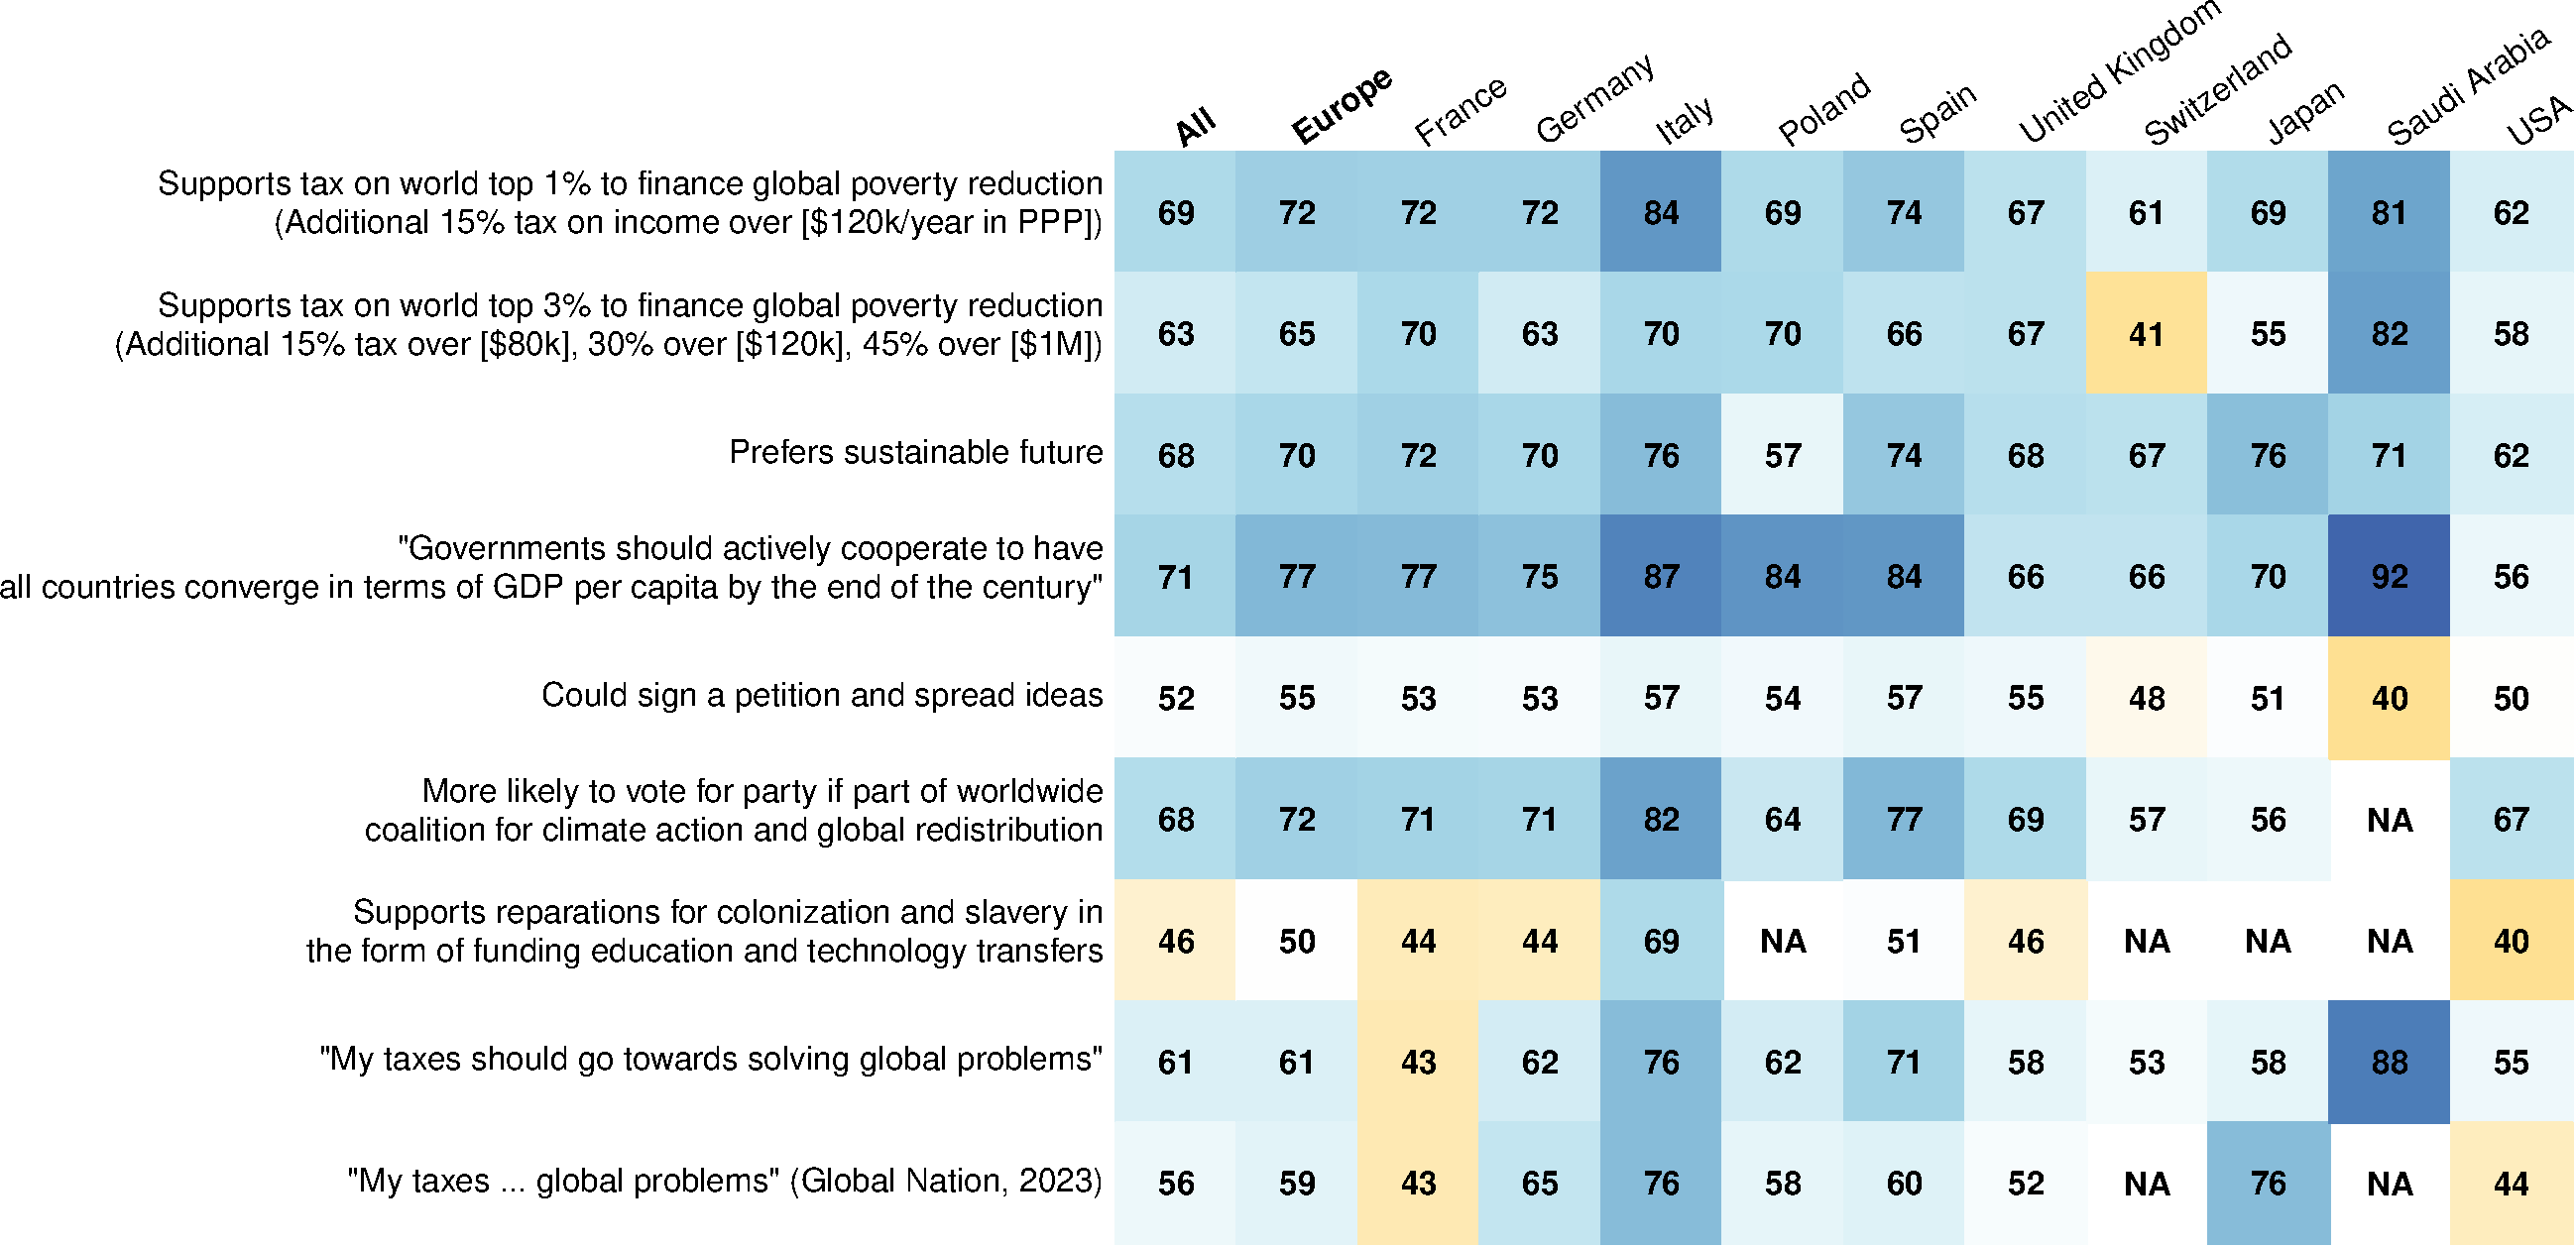
\includegraphics[width=\textwidth]{../figures/country_comparison/radical_redistr_all_share.pdf}} % radical_redistr_share
\end{figure}

\paragraph{Moral circle.}

Asked ``Which group of people do you advocate for when you vote?'',\footnote{In Russia and Saudi Arabia, the question was asked differently. It read: ``Which group do you advocate for? For example, if you were the richest person on Earth, which group would you predominantly help with your money?''\label{fn:group_defended}} 
46\% choose a universalist answer (``Humans'' or ``Sentient beings (humans and animals)''), which is more that the most common answer, that refers to one's fellow citizens (33\%). Universalists are fewer in Japan (30\%) and the U.S. (43\%) but they represent a  majority in Europe (50\%), Russia and Saudi Arabia (57\%), as shown in Figures \ref{fig:group_defended} and \ref{fig:group_defended_all}.
Of people who lean on the left, 59\% are universalists, compared to 32\% on the right or far right. %, and 45\% of non-voters.

% # 10. group_defended: barresN or barres? 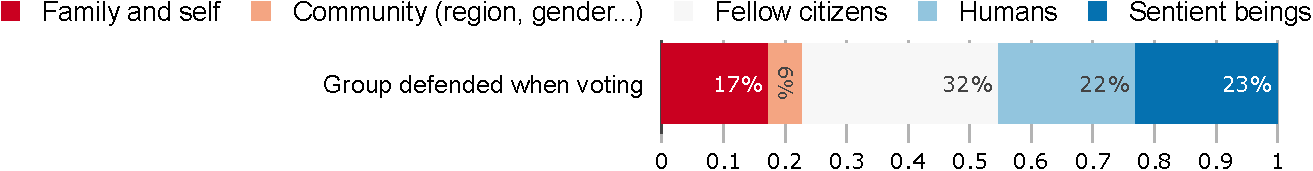
\includegraphics[height=.9\textheight]{../figures/all/group_defended}
\begin{figure}[h!]
    \caption[Moral circle]{``Which group of people do you advocate for when you vote?''\footref{fn:group_defended} (Question \ref{q:group_defended}).
    }\label{fig:group_defended}
    \makebox[\textwidth][c]{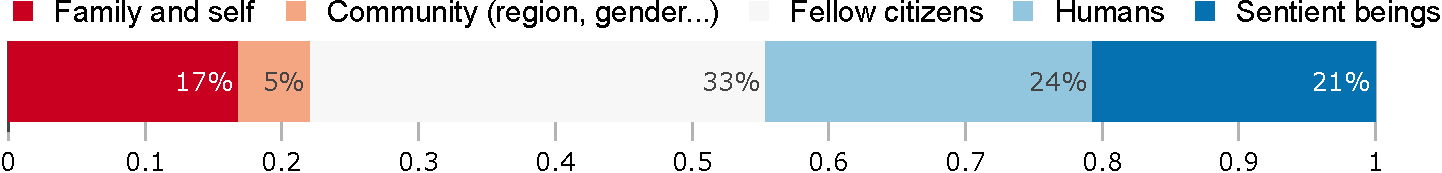
\includegraphics[width=.9\textwidth]{../figures/all/group_defended_nolabel.pdf}} 
\end{figure}

\subsection{Preferred channels to transfer resources to LICs}\label{subsec:transfer_how}

Asked to evaluate the ways to transfer resources to reduce poverty in LICs on a 4-Likert scale, the most preferred option in every country is ``Cash transfers to parents (child allowances), to the disabled and to the elderly'', with 14\% selecting it as the \textit{Best way} overall, and 46\% as a \textit{Right} or \textit{Best way} (Figures \ref{fig:transfer_how}, \ref{fig:transfer_how_above_one}-\ref{fig:transfer_how_negative}). ``Unconditional transfers to the national government'' is the only option seen as a \textit{Wrong way} by the majority, but this share falls from 54\% down to 22\% (and becomes the third most supported option out of seven) when ``transfers to the national government [are] conditioned on the use of funds for poverty reduction programs''. Interestingly, ``Unconditional cash transfers to each household'' are controversial, as they are the second most chosen \textit{Best way} but 36\% view them as a \textit{Wrong way}. Conversely, ``Transfers to public development aid agencies which then finance suitable projects'' is uncontroversial, as only 15\% find it a \textit{Wrong way} \textit{versus} 40\% a \textit{Right} or \textit{Best way}.

% # 11. transfer_how: heatmap (maybe just one row grouping all countries and options in columns) 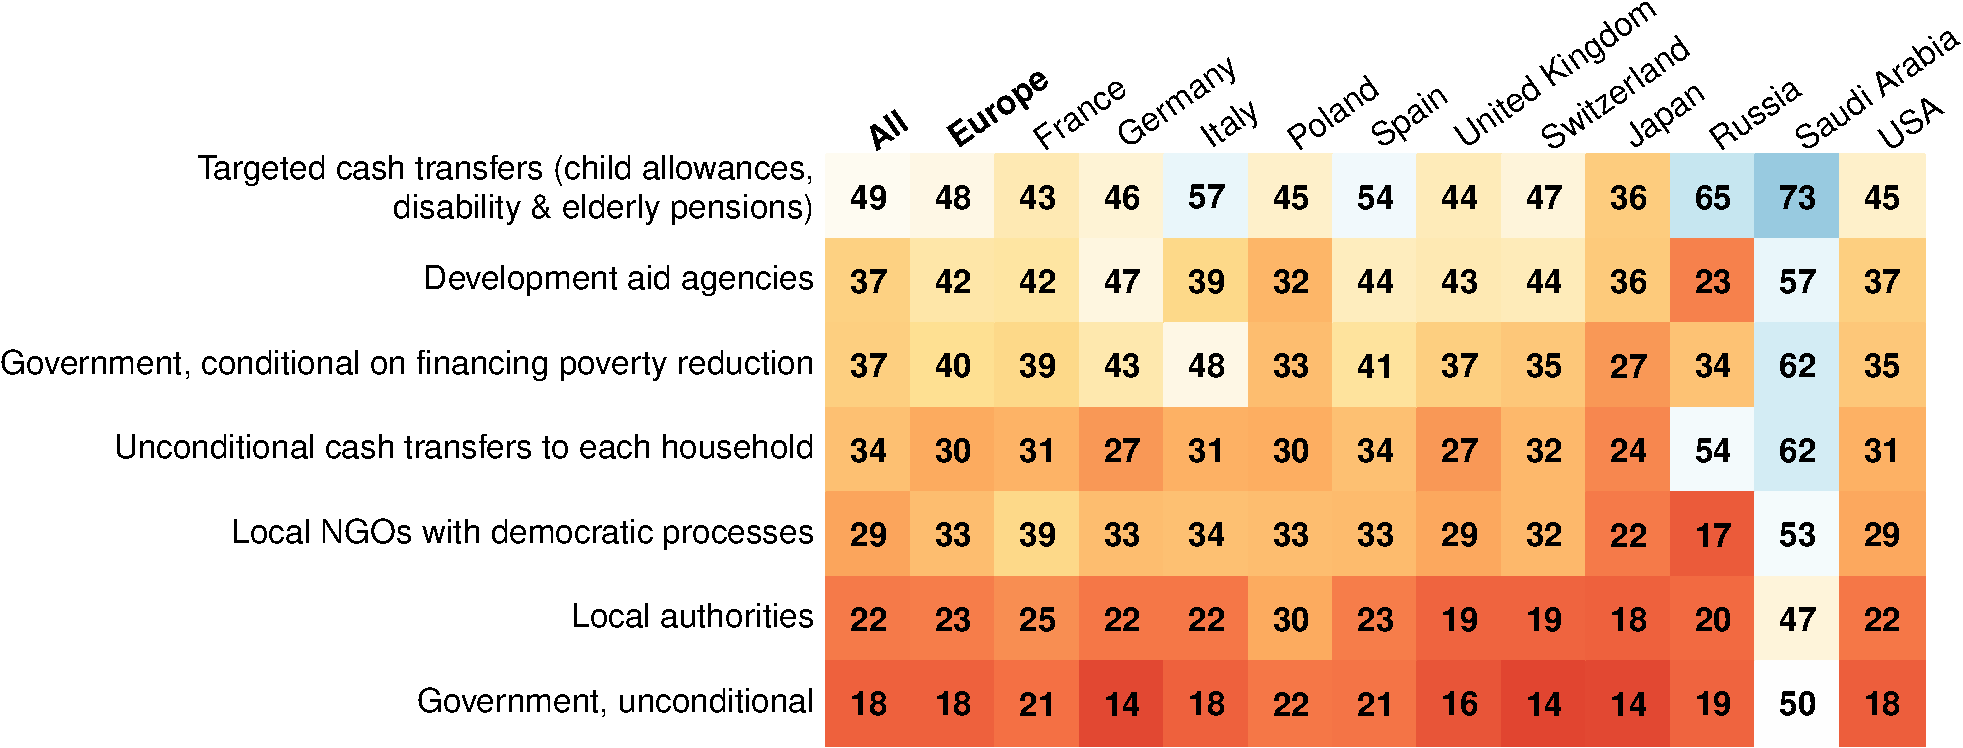
\includegraphics[width=\textwidth]{../figures/country_comparison/transfer_how_positive}
\begin{figure}[h!]
    \caption[\textit{Right} or \textit{Best way} to transfer resources to LICs (global average)]{``How do you evaluate each of these channels to transfer resources to reduce poverty in LICs?''\\ Percentage of \textit{Right} or \textit{Best} way (other options: \textit{Wrong} or \textit{Acceptable way}). (Question \ref{q:transfer_how}).
    }\label{fig:transfer_how}
    \makebox[\textwidth][c]{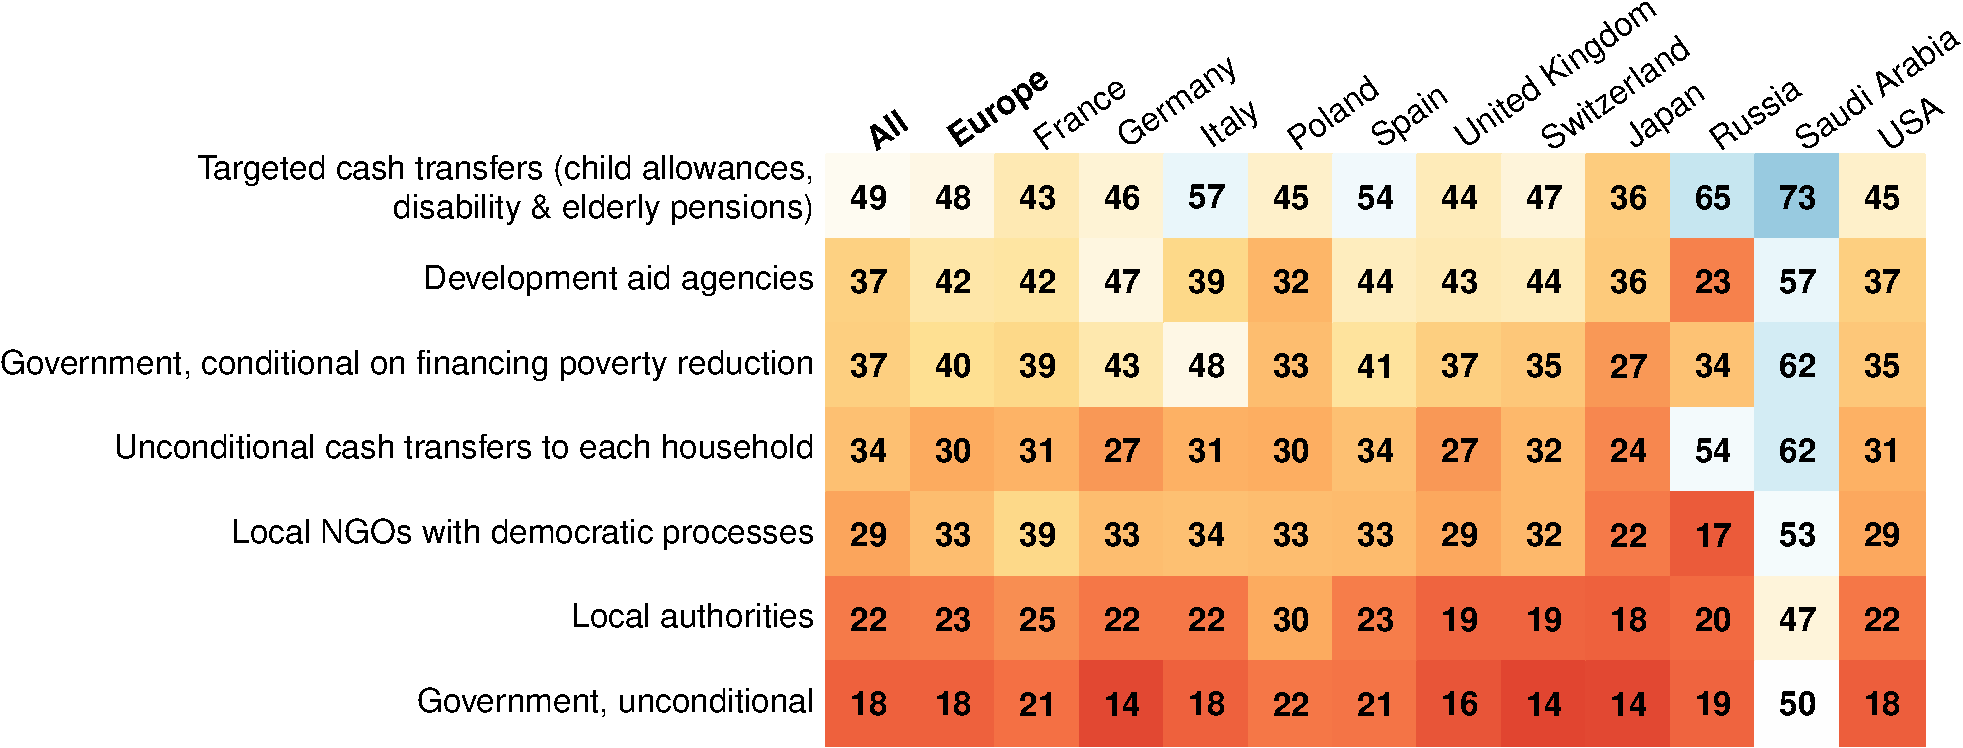
\includegraphics[width=\textwidth]{../figures/country_comparison/transfer_how_positive.pdf}} 
\end{figure}

\subsection{Custom global income redistribution}\label{subsec:custom_redistr}

The last task of the questionnaire allowed respondents to play with the shape of the global income distribution. The question text includes the following instructions: 
\begin{quote}``Below you will find a graph of the world distribution of after-tax income and three sliders that vary it. The current distribution is in red, and your custom one is in green. The first two sliders control the proportion of winners and the proportion of losers, among all humans. The third slider controls the degree of redistribution from the richest to the poorest. % TODO say whether it's in PPP
If you do not want new policies to reduce global inequality, you can set the third slider to zero.''\end{quote} 
The interactive question is available on \href{https://bit.ly/custom_redistr}{bit.ly/custom\_redistr} and the algorithm to translate sliders' positions into a redistribution is described in Appendix \ref{app:algo}. %and a video explainer on TODO.
Figure \ref{fig:custom_redistr_question} displays what respondents see below the instructions, including the interactive graph and a table summarizing how their custom redistribution would affect five example income levels (including their own, asked right before). To dampen a potential anchoring at sliders' initial positions,%
\footnote{To test for anchoring, I regress responses on the sliders' initial position. %The initial positions have a significant anchoring effect on the responses. %Relative to the other variant's %difference between the two variants' 
% initial positions, a given variant brings the responses closer to its position by 
The anchoring effect, defined as the effect size relative to the difference between the two variants' initial positions, is always significant, at 40\% for the share of winners, 55\% for the share of losers, and 42\% for the degree of redistribution. While anchoring plays a role, the responses converge to a middle point between the two anchors, indicating that the anchors themselves may have been defined by the surveyor (myself) drifting away (in opposite directions) from a shared preference. % collective, common taste or natural focal point. 
} 
the sliders have two random initial positions: %  (yielding similar rich-to-poor transfers of 4.3\% to 4.6\% of the world GDP)
either %the \textit{diffuse} redistribution with 
60\% of winners, 20\% of losers, and a degree of redistribution of 2 out of 10 (as in Figure \ref{fig:custom_redistr_question}); or %the \textit{concentrated} one with 
40\%, 10\%, and 7/10, respectively. 
As the task is difficult to understand (and not so handy %to handle 
on phone screens), respondents are instructed that they can skip it. 

% # 12. average custom_redistr 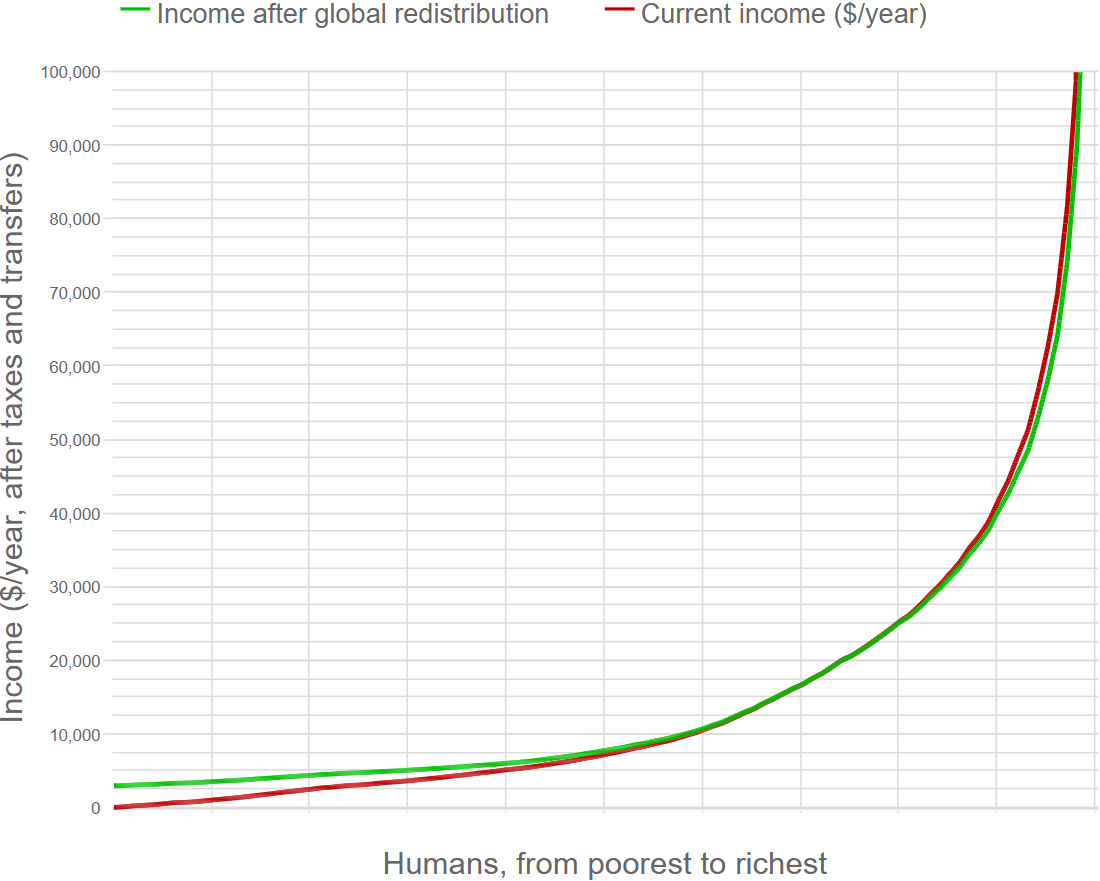
\includegraphics[height=.8\textheight]{../figures/all/custom_redistr_mean.png}
\begin{figure}[h!]
   \caption[Custom redistribution task screenshot]{Custom global redistribution: screenshot of the bottom of the page. (Question \ref{q:custom_redistr}).
    }\label{fig:custom_redistr_question}
    \makebox[\textwidth][c]{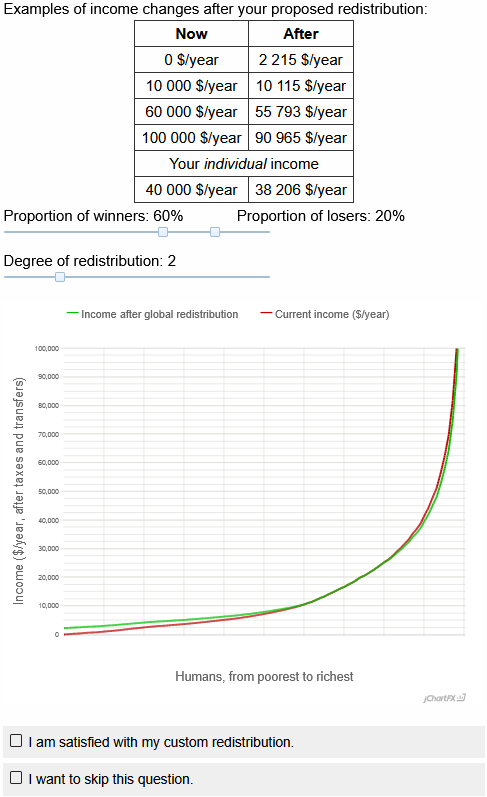
\includegraphics[height=.85\textheight]{../figures/questionnaire/survey_custom_redistr_bottom.png}} % bottom2 is without the choice options satisfied/skip
\end{figure}

Overall, 56\% are satisfied with their custom redistribution and 43\% skip it. 
% Furthermore, 35\% of the respondents did not move the sliders from their original position, and while 39\% of them still state that they are satisfied with the redistribution, I exclude them from the main analysis, conducted over the 40\% of ``conforming'' % responsive, admitted, 
% respondents who touched the sliders and are satisfied with their custom redistribution. 
While the non-response rate may seem high, it is relatively spread out over the population. Indeed, the share of satisfied respondents is 52\% for non-voters, 54\% for center-right or right-wing voters, 57\% for far right voters and 61\% for left-wing voters; while it ranges from 49\% for people without a %secondary education (i.e. 
high-school diploma to 57\% for those with a post-secondary diploma.
% While the non-response rate may seem high, it is relatively spread out over the population. Indeed, the share of conforming respondents is 37\% for non-voters, 39\% for center-right or right-wing voters, 40\% for far right voters and 43\% for left-wing voters; while it ranges from 33\% for people without a high-school diploma to 42\% for those with a post-secondary diploma.  
The limited heterogeneity in response rates across crucial sociodemographics suggests that the task enabled motivated respondents to make an informed choice regarding their preferred redistribution with little sacrifice in terms of sample representativeness.

% \paragraph{Anchoring}
% Furthermore, the average responses are similar between satisfied and all respondents: between these groups, the share of winners and the degree of redistribution differ by at most 2\%, and the share of losers by at most 10\%. The similarity in results between satisfied respondents who moved the sliders and those who did not means that the average custom responses are similar to the average between the two possible sliders' initial positions. Two factors may explain this similarity. First, the responses might have been anchored at sliders' initial positions. Second, both the respondents and the surveyor (myself) might have a similar view of what a reasonable redistribution looks like. To test for anchoring, I regress responses on the sliders' initial position. The initial positions have a significant anchoring effect on the responses. %Relative to the other variant's %difference between the two variants' 
% % initial positions, a given variant brings the responses closer to its position by 
% The anchoring effect, defined as the effect size relative to the difference between the two variants' initial positions, is 
% 40\% for the share of winners, 55\% for the share of losers, and 42\% for the degree of redistribution. While anchoring plays a role, the responses converge to a middle point between the two anchors, indicating that the anchors themselves may have been defined by the surveyor drifting away (in opposite directions) from a shared preference. % collective, common taste or natural focal point. 

% To sum up, while this task enables respondents to make an informed choice regarding their preferred redistribution, it remains an imperfect method, and more appropriate ways to reveal citizens' preferred redistribution may be proposed. % TODO: change this paragraph

% With these caveats in mind, 
Figure \ref{fig:custom_redistr_median} shows the median preferred redistribution among satisfied respondents, i.e. the curve obtained by setting the sliders at their median preferred values: 49\% of winners, 18\% of losers, and a degree of redistribution of 5/10, resulting in a transfer from rich-to-poor at 5.4\% of world income and in a minimum income of \$287 per month. 
Interestingly, 48\% choose to lose from their custom redistribution while only 9\% choose to win, the median satisfied respondent choosing parameters such that they neither win nor lose. Besides, 10\% of satisfied respondents choose the status quo, preserving the current income distribution. 
Finally, Figure \ref{fig:custom_redistr_mean} presents the average preferred redistribution among conforming respondents (i.e. the curve obtained by pointwise-averaging custom curves). % TODO fill mean_custom_redistr_stats, compute mean transfer by variant
% TODO distribution of min_income and transfer
The average preferred redistribution transfers 5.4\% of world income % TODO: harmonize: world income or world GDP?
from the top 27\% to the bottom 73\%, and entails a minimum income of \$247 per month.  % TODO by country
As shown in Figure \ref{fig:tax_radical_redistr}, at the top of the distribution, the average preferred redistribution can be obtained from a 7\% marginal income tax rate above \$25,000 and a 16\% rate above \$40,000 per year (at Purchasing Power Parity). 

\cite{fabre_french_2022} applied the same method to uncover French preferences regarding national income redistribution, and tested the support for the median and average % 42% losers in French average
preferred redistributions on a separate sample. Excluding the 22\% to 24\% of people not responding, the 51\% supported the average redistribution and 67\% the median one.\footnote{\cite{fabre_french_2022} also tested a redistribution obtained from median parameters and a 5\% lower GDP to account for adverse behavioral responses: it was supported by 62\% of French respondents.} 
While one cannot be sure that these results would replicate in the context of a global redistribution, they suggest that the average or median redistributions described above might be accepted by a majority.

\section{Conclusion} % Summary, conclusion


% Appendix TODO
% - Influenced by question on revenue splits and NCQG / more or less consistent on NCQG


% \begin{methods}  % WPcomment
  \begin{small} % NCCcomment
%Put methods in here.  If you are going to subsection it, use \subsection commands.  Methods section should be less than 800 words and if it is less than 200 words, it can be incorporated into the main text.
\section*{\normalsize Methods}\label{sec:methods} % NCCcomment
\addcontentsline{toc}{section}{\nameref{sec:methods}}

% The paper utilizes two sets of surveys: the \textit{global} survey and the \textit{Western} surveys. The \textit{global} surveys consist of two U.S. surveys, \textit{US1} and \textit{US2}, and one European survey, \textit{Eu}. The \textit{global} survey was conducted from March 2021 to March 2022 on 40,680 respondents from 20 countries (with 1,465 to 2,488 respondents per country). \textit{US1} collected responses from 3,000 respondents between January and March 2023, while \textit{US2} gathered data from 2,000 respondents between March and April 2023. \textit{Eu} included 3,000 respondents and was conducted from February to March 2023. We used the survey companies \emph{Dynata} and \emph{Bilendi}. To ensure representative samples, we employed stratified quotas based on gender, age (5 brackets), income (4), region (4), education level (3), and ethnicity (3) for the U.S. We also incorporated survey weights throughout the analysis to account for any remaining imbalances. These weights were constructed using the quota variables as well as the degree of urbanization, and trimmed between 0.25 and 4. Stratified quotas followed by reweighting is the usual method to reduce selection bias from opt-in online panels, when better sampling methods (such as compulsory participation of random dwellings) are unavailable.\cite{scherpenzeel_how_2010} By applying weights, the results are fully representative of the respective countries along the above mentioned dimensions. %. 
% Appendix \ref{app:balance} shows that the treatment branches are balanced. Appendix \ref{app:placebo} runs placebo tests of the effects of each treatment on unrelated outcomes. We do not find effects of earlier treatments on unrelated outcomes arriving later in the survey. Appendix \ref{app:extended} shows that our results are unchanged when including inattentive respondents.

\section*{\normalsize Acknowledgements}
bla

% \section*{\normalsize Competing interests} Fabre declares that he also serves as treasurer of Global Redistribution Advocates.

% \end{methods} % WPcomment
\end{small}  % NCCcomment

% \bibliographystyle{naturemag_noURL} % nature class works only with style naturemag or naturemag_noURL, and naturemag bugs if there are certain URLs (like .pdf). Also, nature class only works with \cite, not \citet or \citep.  % WPcomment
\renewcommand{\url}[1]{\href{#1}{Link}} % NCCcomment
% \bibliographystyle{unsrtnat} % NCCcomment
% \bibliography{global_tax_attitudes}

\clearpage

\putbib
\end{bibunit}

\begin{bibunit}[plainnaturl_clean]

\appendix % NCCcomment
% \renewcommand{\thetable}{ED\arabic{table}}
% \renewcommand{\thefigure}{ED\arabic{figure}}
% \setcounter{figure}{0}
% \setcounter{table}{0}


\renewcommand{\thetable}{S\arabic{table}}
\renewcommand{\thefigure}{S\arabic{figure}}
\setcounter{figure}{0}
\setcounter{table}{0}

\clearpage
\section{Raw results% from the complementary surveys
}\label{app:raw_results}

% Country-specific raw results are also available as supplementary material files:  \href{https://github.com/bixiou/international_attitudes_toward_global_policies/raw/main/paper/app_desc_stats_US.pdf}{US}, \href{https://github.com/bixiou/international_attitudes_toward_global_policies/raw/main/paper/app_desc_stats_EU.pdf}{EU}, \href{https://github.com/bixiou/international_attitudes_toward_global_policies/raw/main/paper/app_desc_stats_FR.pdf}{FR}, \href{https://github.com/bixiou/international_attitudes_toward_global_policies/raw/main/paper/app_desc_stats_DE.pdf}{DE}, \href{https://github.com/bixiou/international_attitudes_toward_global_policies/raw/main/paper/app_desc_stats_ES.pdf}{ES}, \href{https://github.com/bixiou/international_attitudes_toward_global_policies/raw/main/paper/app_desc_stats_UK.pdf}{UK}.

\begin{figure}[h!]
    \caption[Keyword classification of open-ended fields]{Keyword classification of open-ended fields (matches with at least one keyword in a list). (Questions~\ref{q:concerns_field}-\ref{q:injustice_field}). \hfill Back~to~Section~\ref{subsec:considerations}.
    }\label{fig:field_keyword}
    \makebox[\textwidth][c]{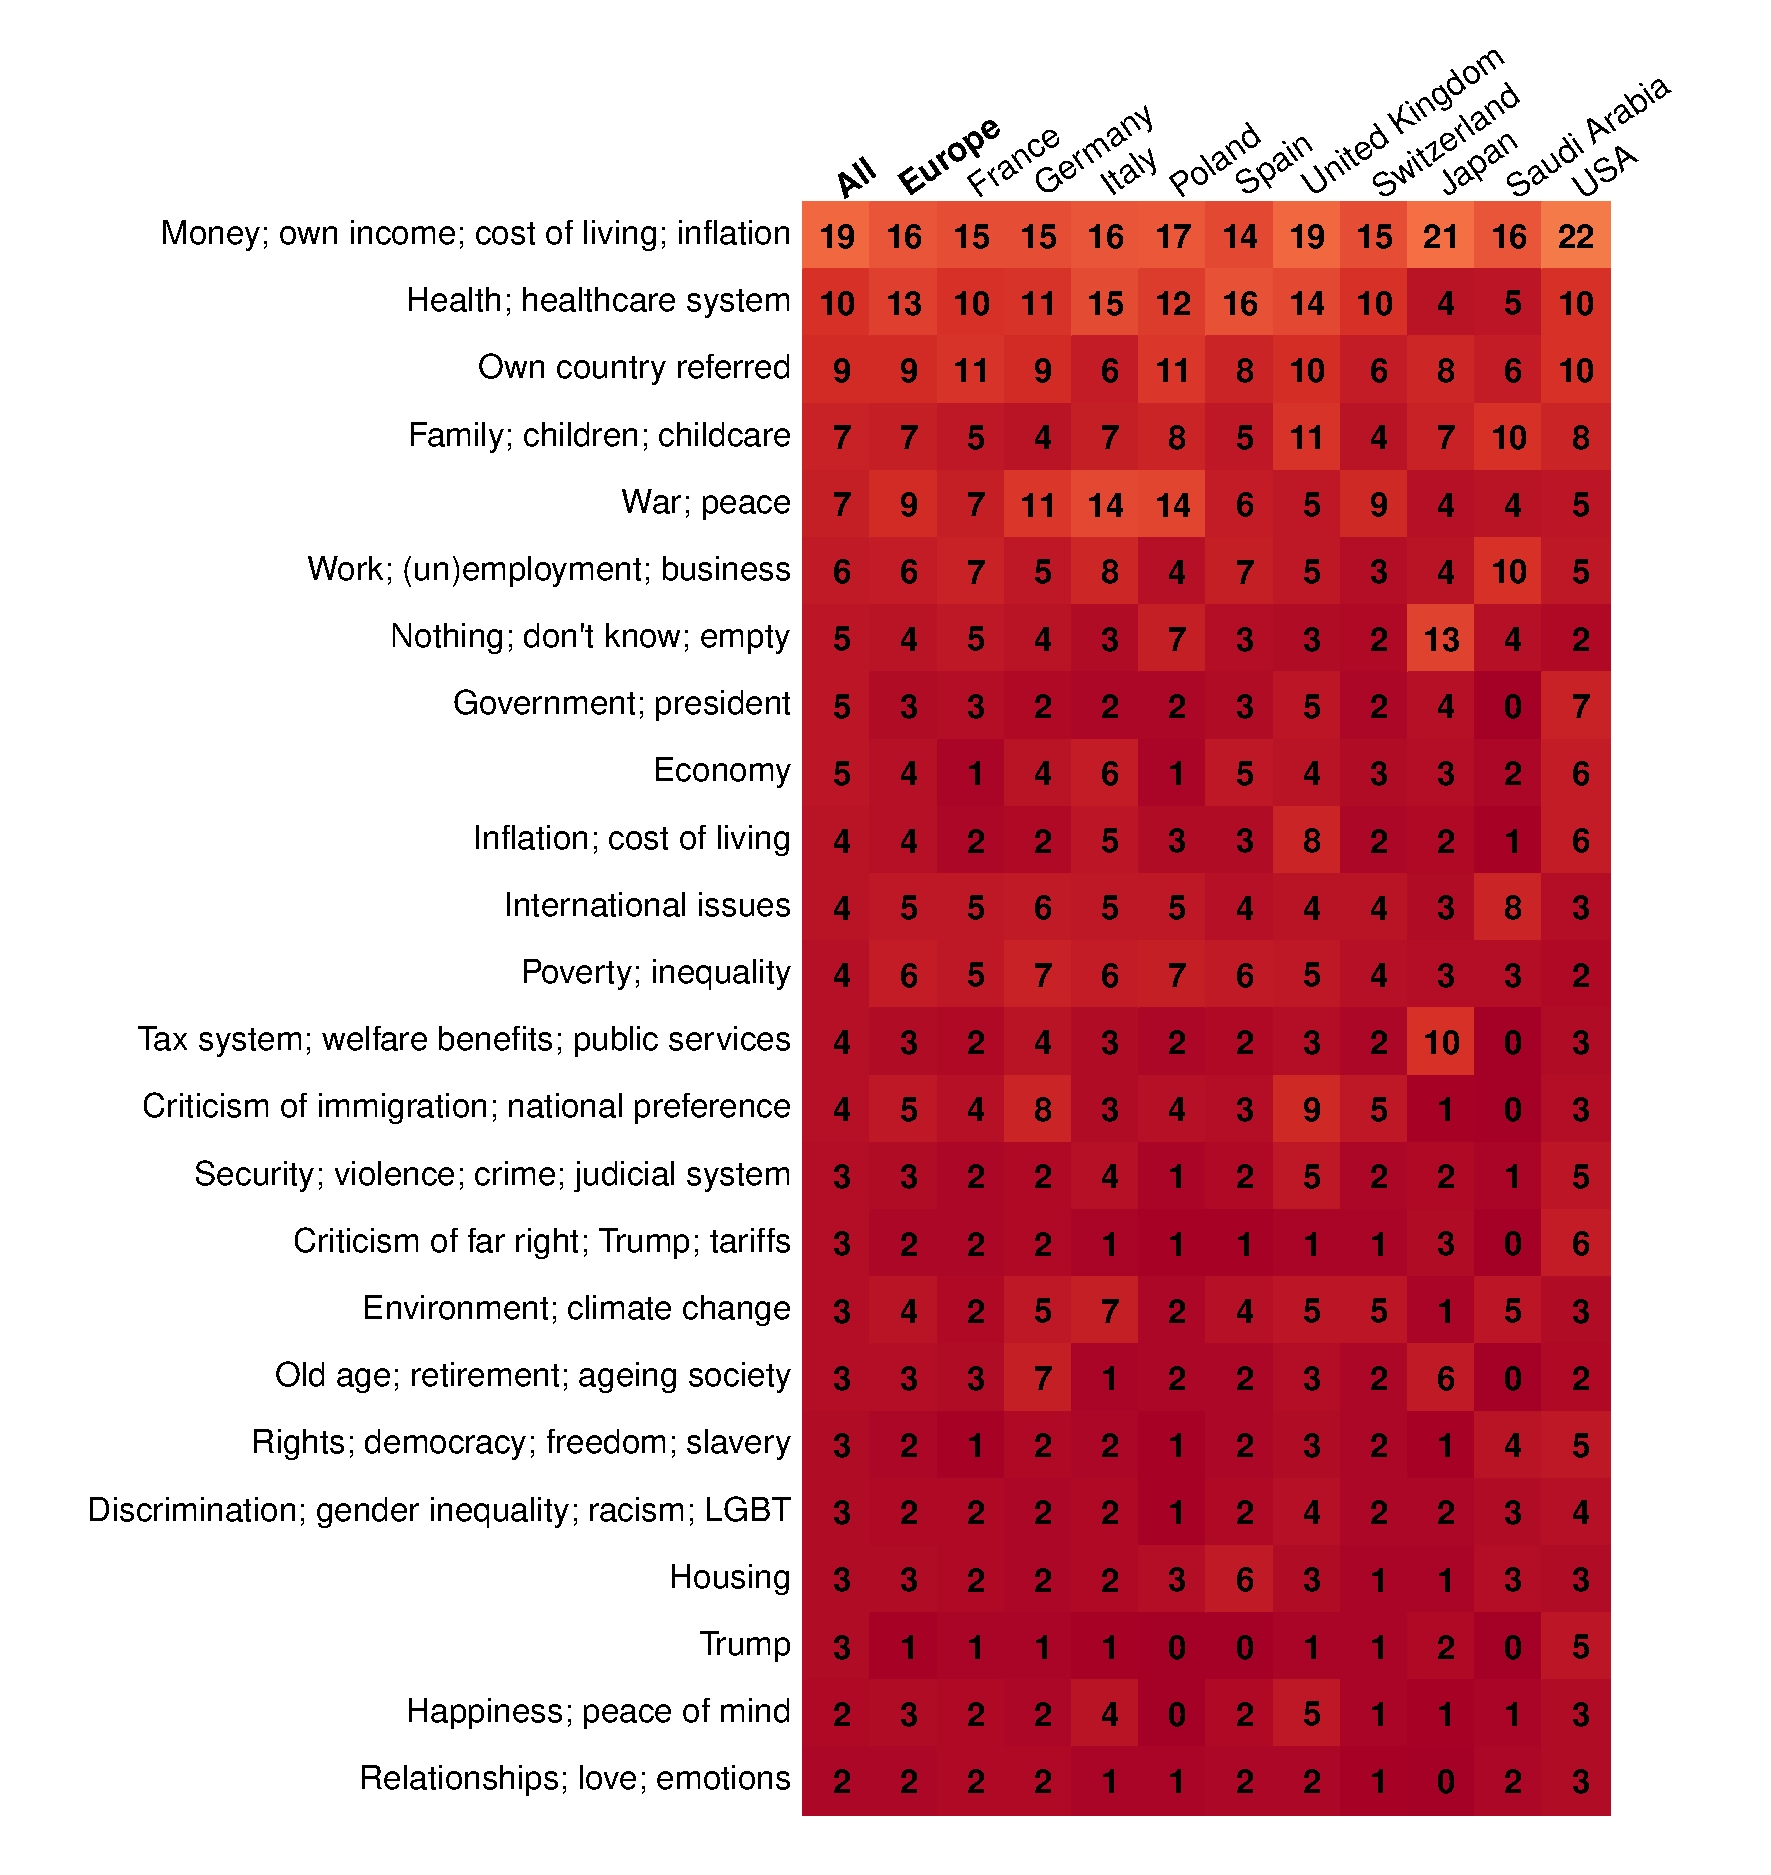
\includegraphics[height=.85\textheight]{../figures/country_comparison/field_keyword_main_positive.pdf}} 
\end{figure}

\begin{figure}[h!]
    \caption[AI classification of open-ended fields]{AI classification of open-ended fields (using ChatGPT-4.1). (Questions~\ref{q:concerns_field}-\ref{q:injustice_field}).\hfill Back~to~Section~\ref{subsec:considerations}.
    }\label{fig:field_gpt}
    \makebox[\textwidth][c]{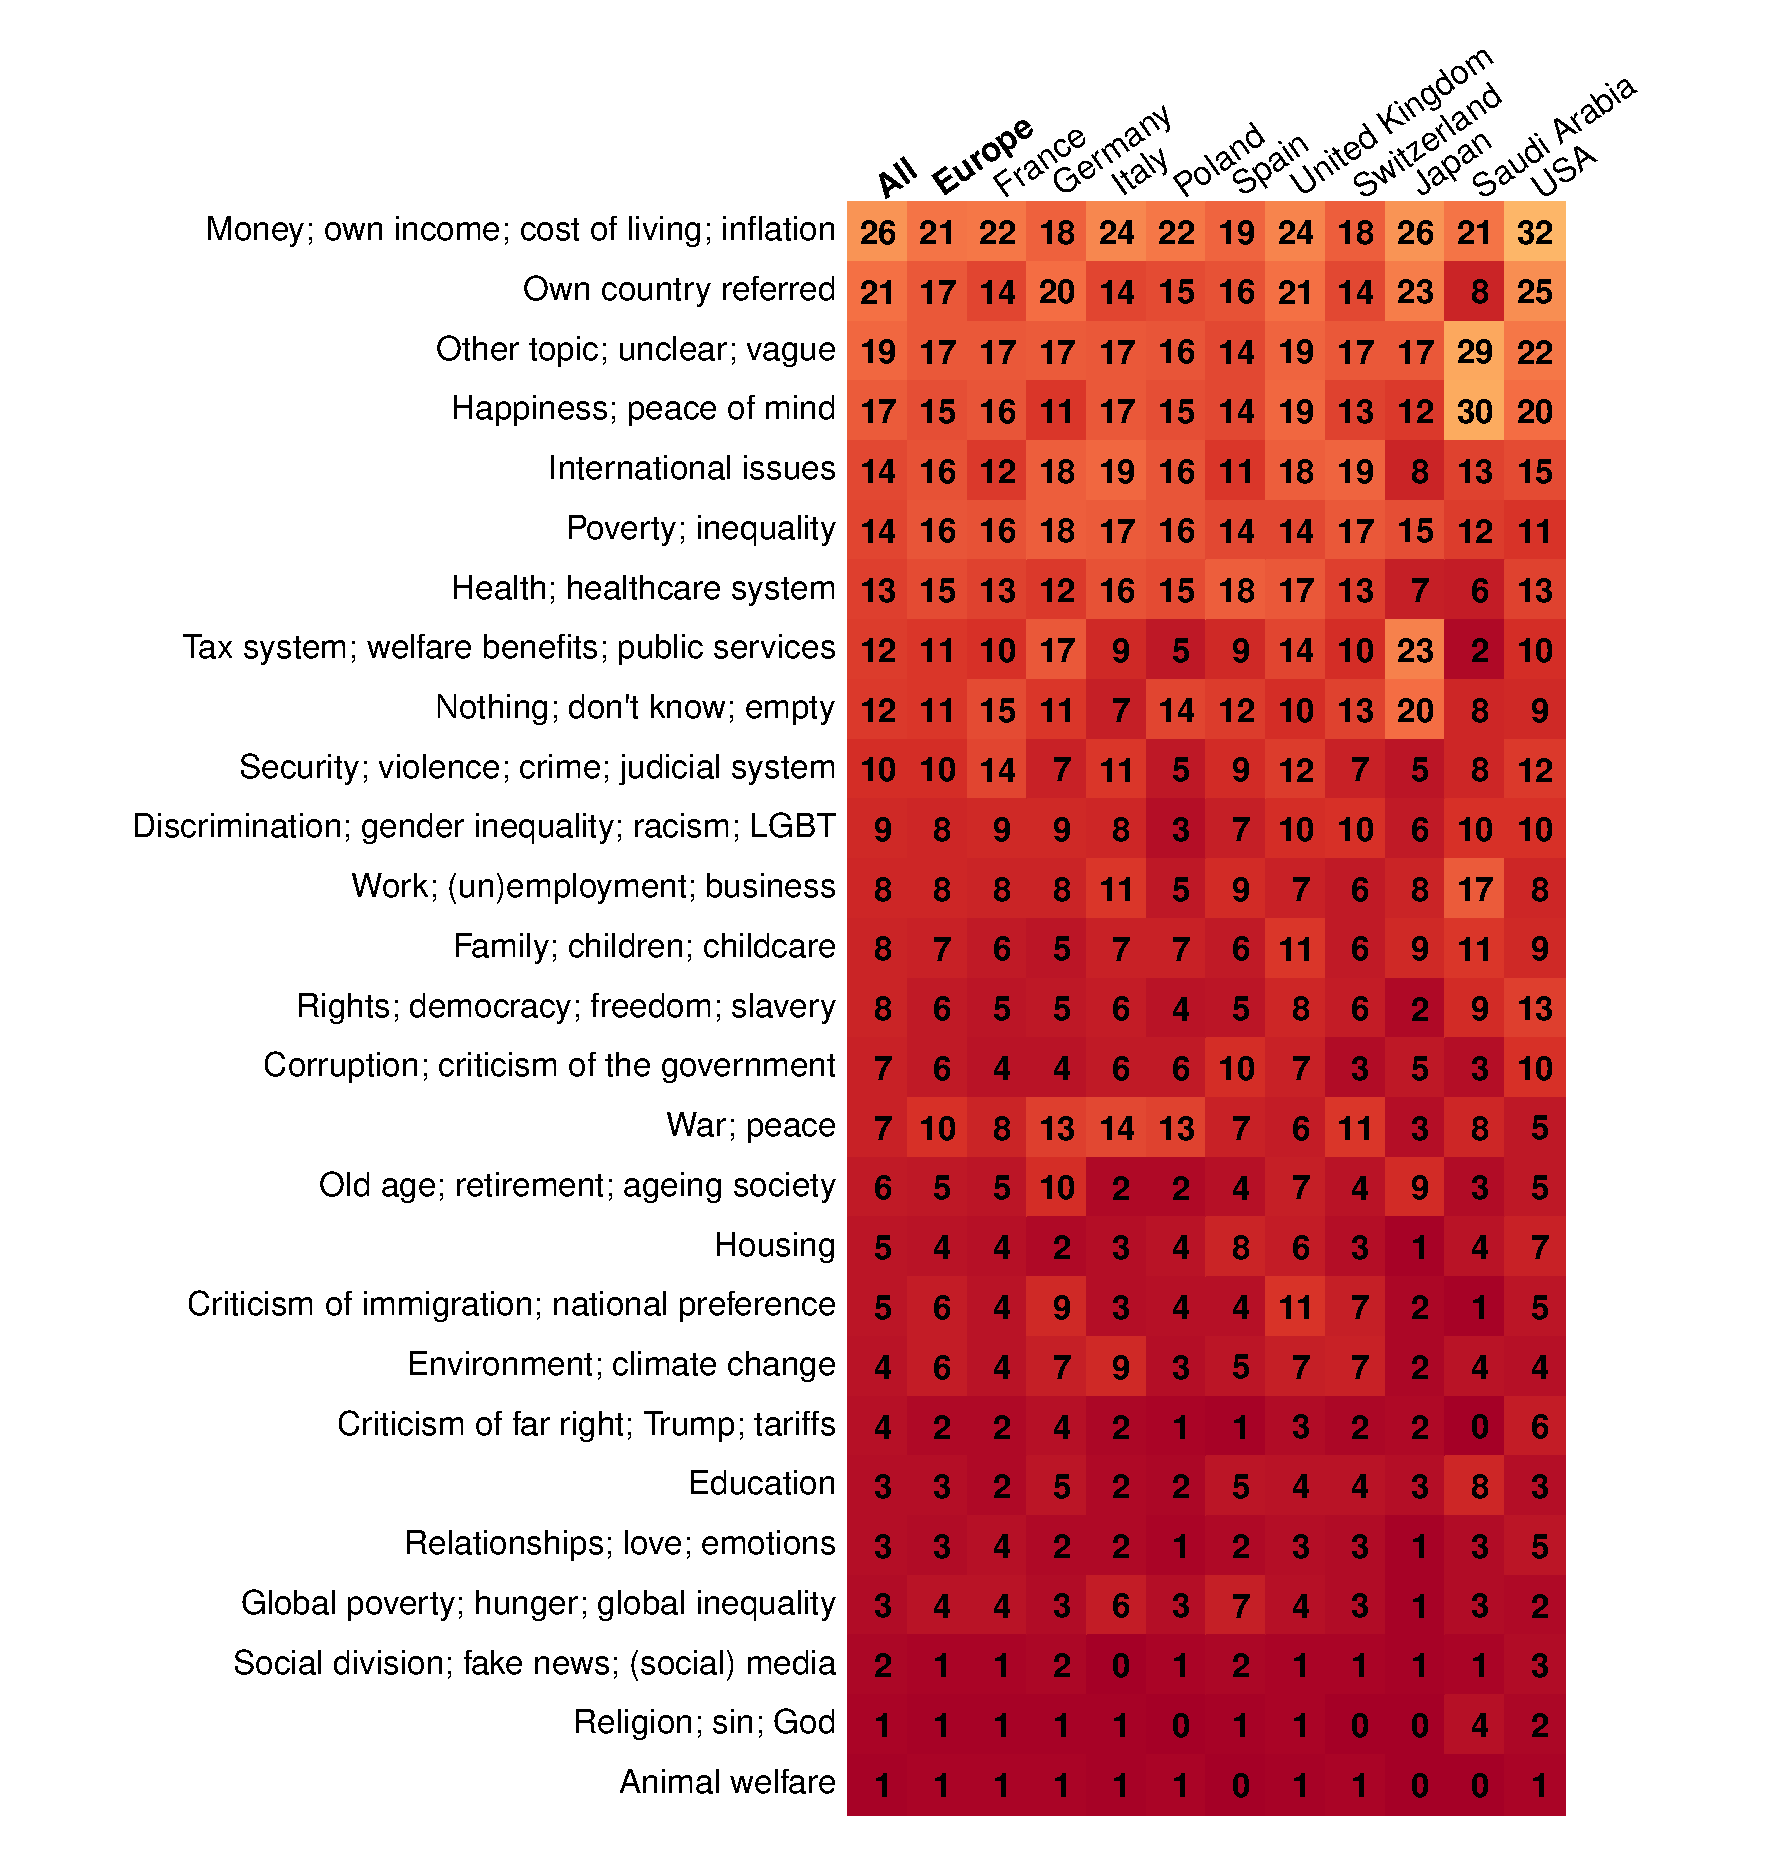
\includegraphics[height=.85\textheight]{../figures/country_comparison/field_gpt_positive.pdf}} 
\end{figure}

\begin{figure}[h!]
    \caption[Manual classification of open-ended fields]{Manual classification of open-ended fields. (Questions~\ref{q:concerns_field}-\ref{q:injustice_field}).\hfill Back~to~Section~\ref{subsec:considerations}.
    }\label{fig:field_manual}
    \makebox[\textwidth][c]{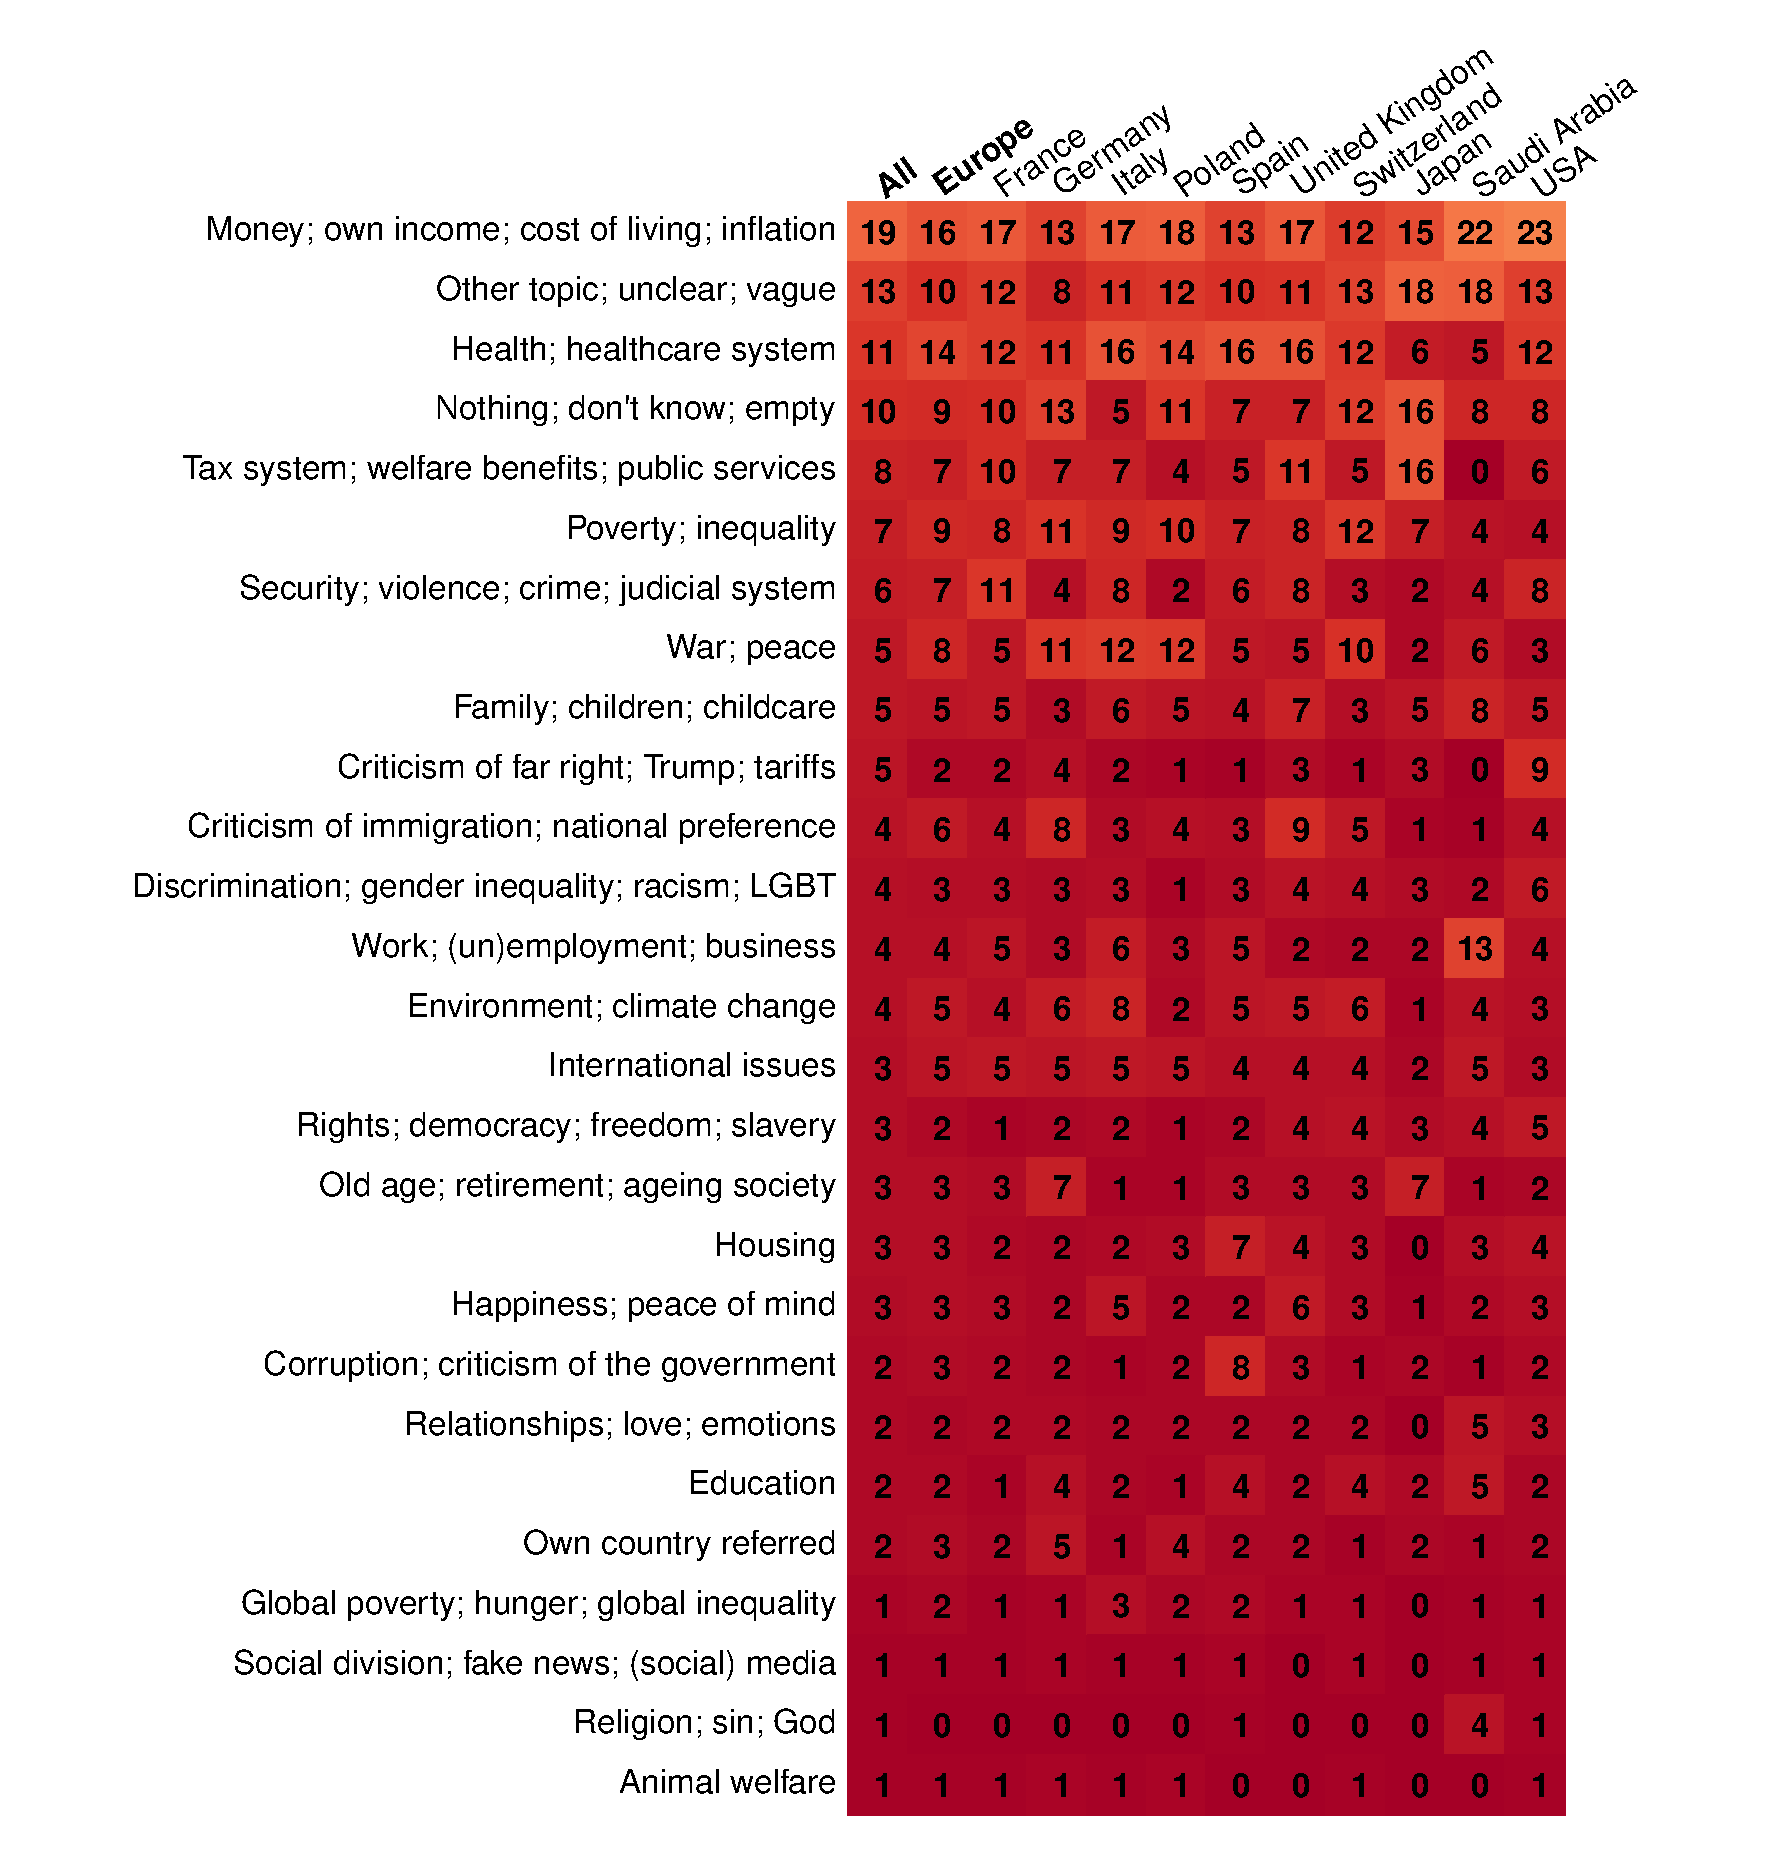
\includegraphics[height=.85\textheight]{../figures/country_comparison/field_manual_positive.pdf}} 
\end{figure}

\begin{figure}[h!]
    \caption[Manual classification of \textit{concerns} fields]{Manual classification of \textit{concerns} fields: ``What are your main concerns these days?'' (Question~\ref{q:concerns_field}).\hfill Back~to~Section~\ref{subsec:considerations}.
    }\label{fig:concerns_field}
    \makebox[\textwidth][c]{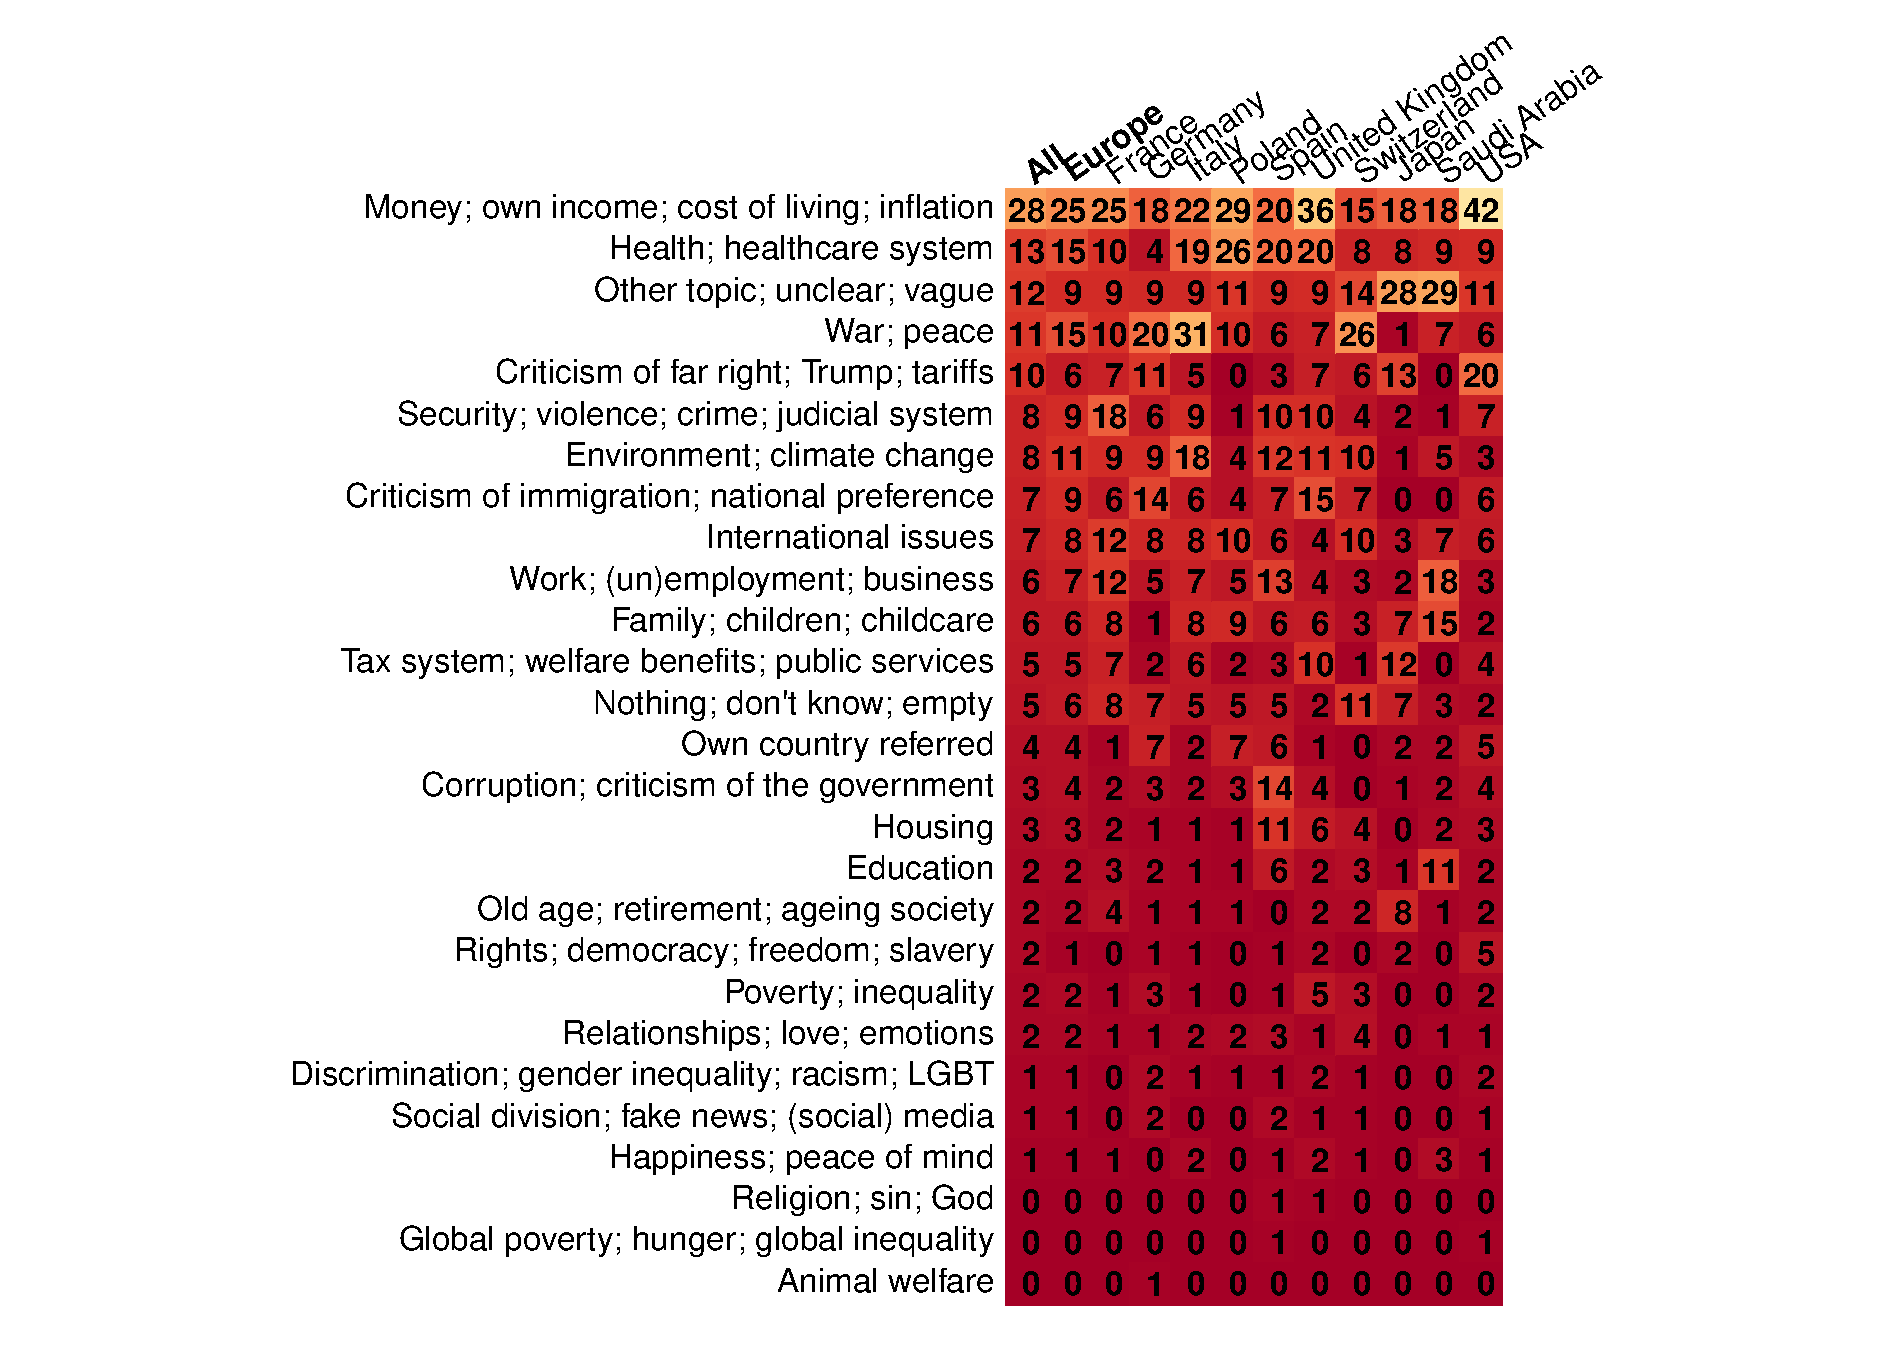
\includegraphics[height=.85\textheight]{../figures/country_comparison/field_concerns_manual_positive.pdf}} 
\end{figure}

\begin{figure}[h!]
    \caption[Manual classification of \textit{wish} fields]{Manual classification of \textit{wish} fields: ``What are your needs or wishes?'' (Question~\ref{q:wish_field}).\hfill Back~to~Section~\ref{subsec:considerations}.
    }\label{fig:wish_field}
    \makebox[\textwidth][c]{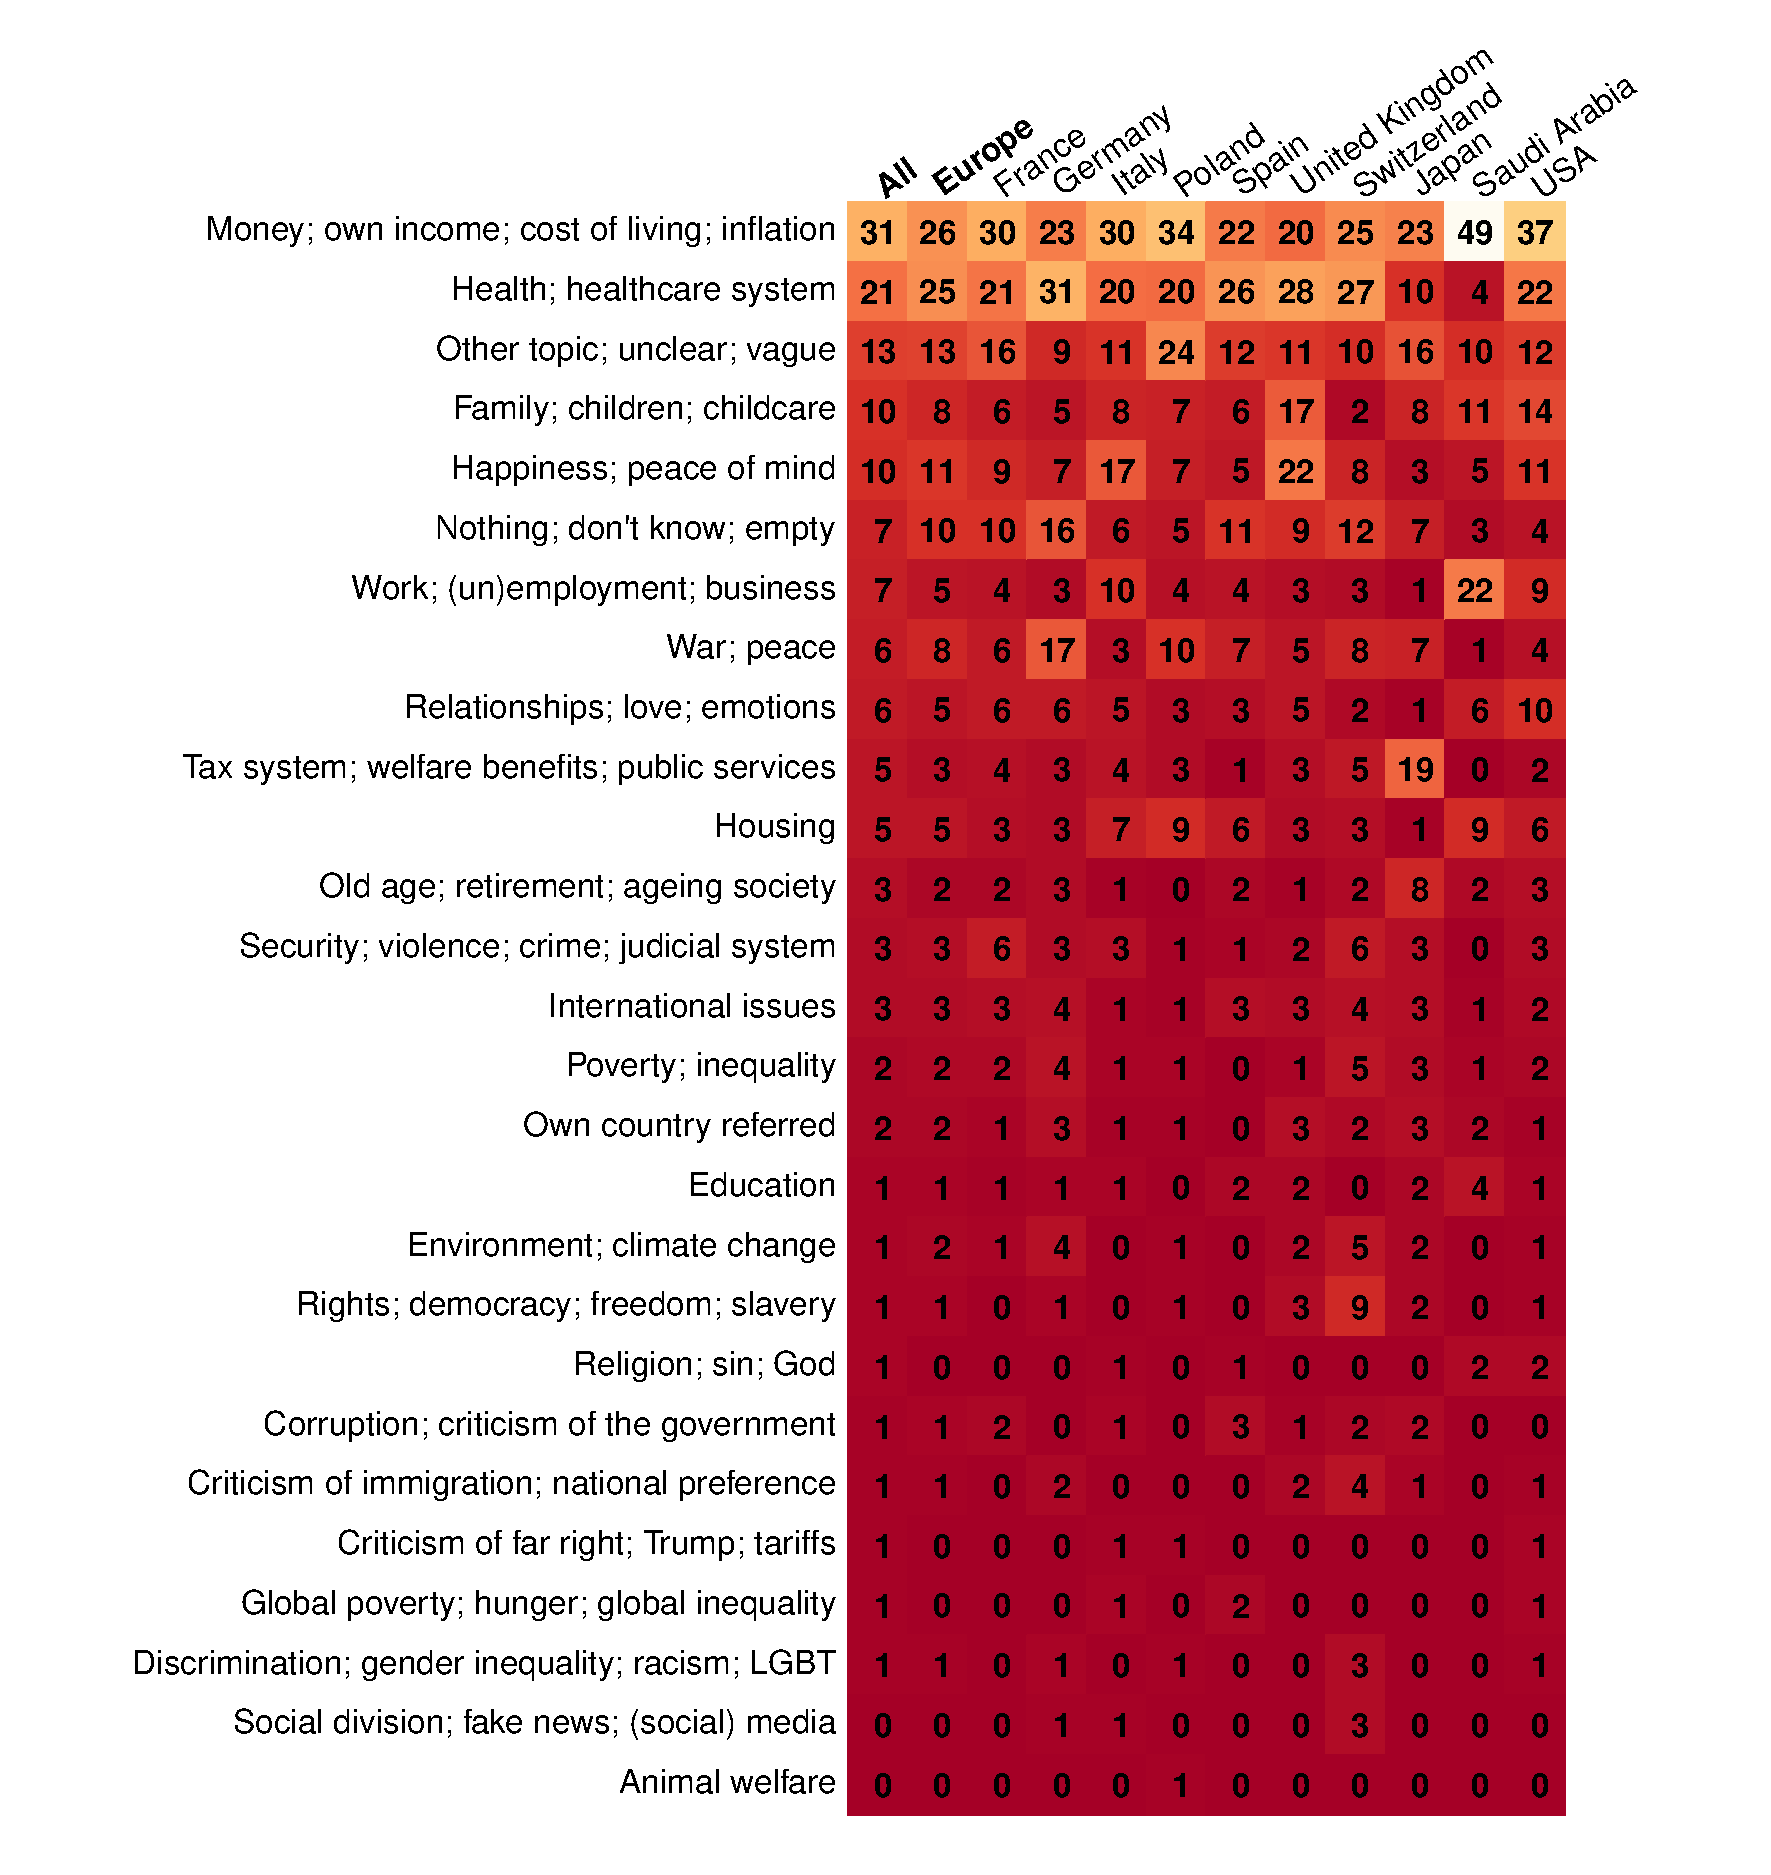
\includegraphics[height=.85\textheight]{../figures/country_comparison/field_wish_manual_positive.pdf}} 
\end{figure}

\begin{figure}[h!]
    \caption[Manual classification of \textit{injustice} fields]{Manual classification of \textit{injustice} fields: ``What according to you is the greatest injustice of all?'' (Question~\ref{q:injustice_field}).\hfill Back~to~Section~\ref{subsec:considerations}.
    }\label{fig:injustice_field}
    \makebox[\textwidth][c]{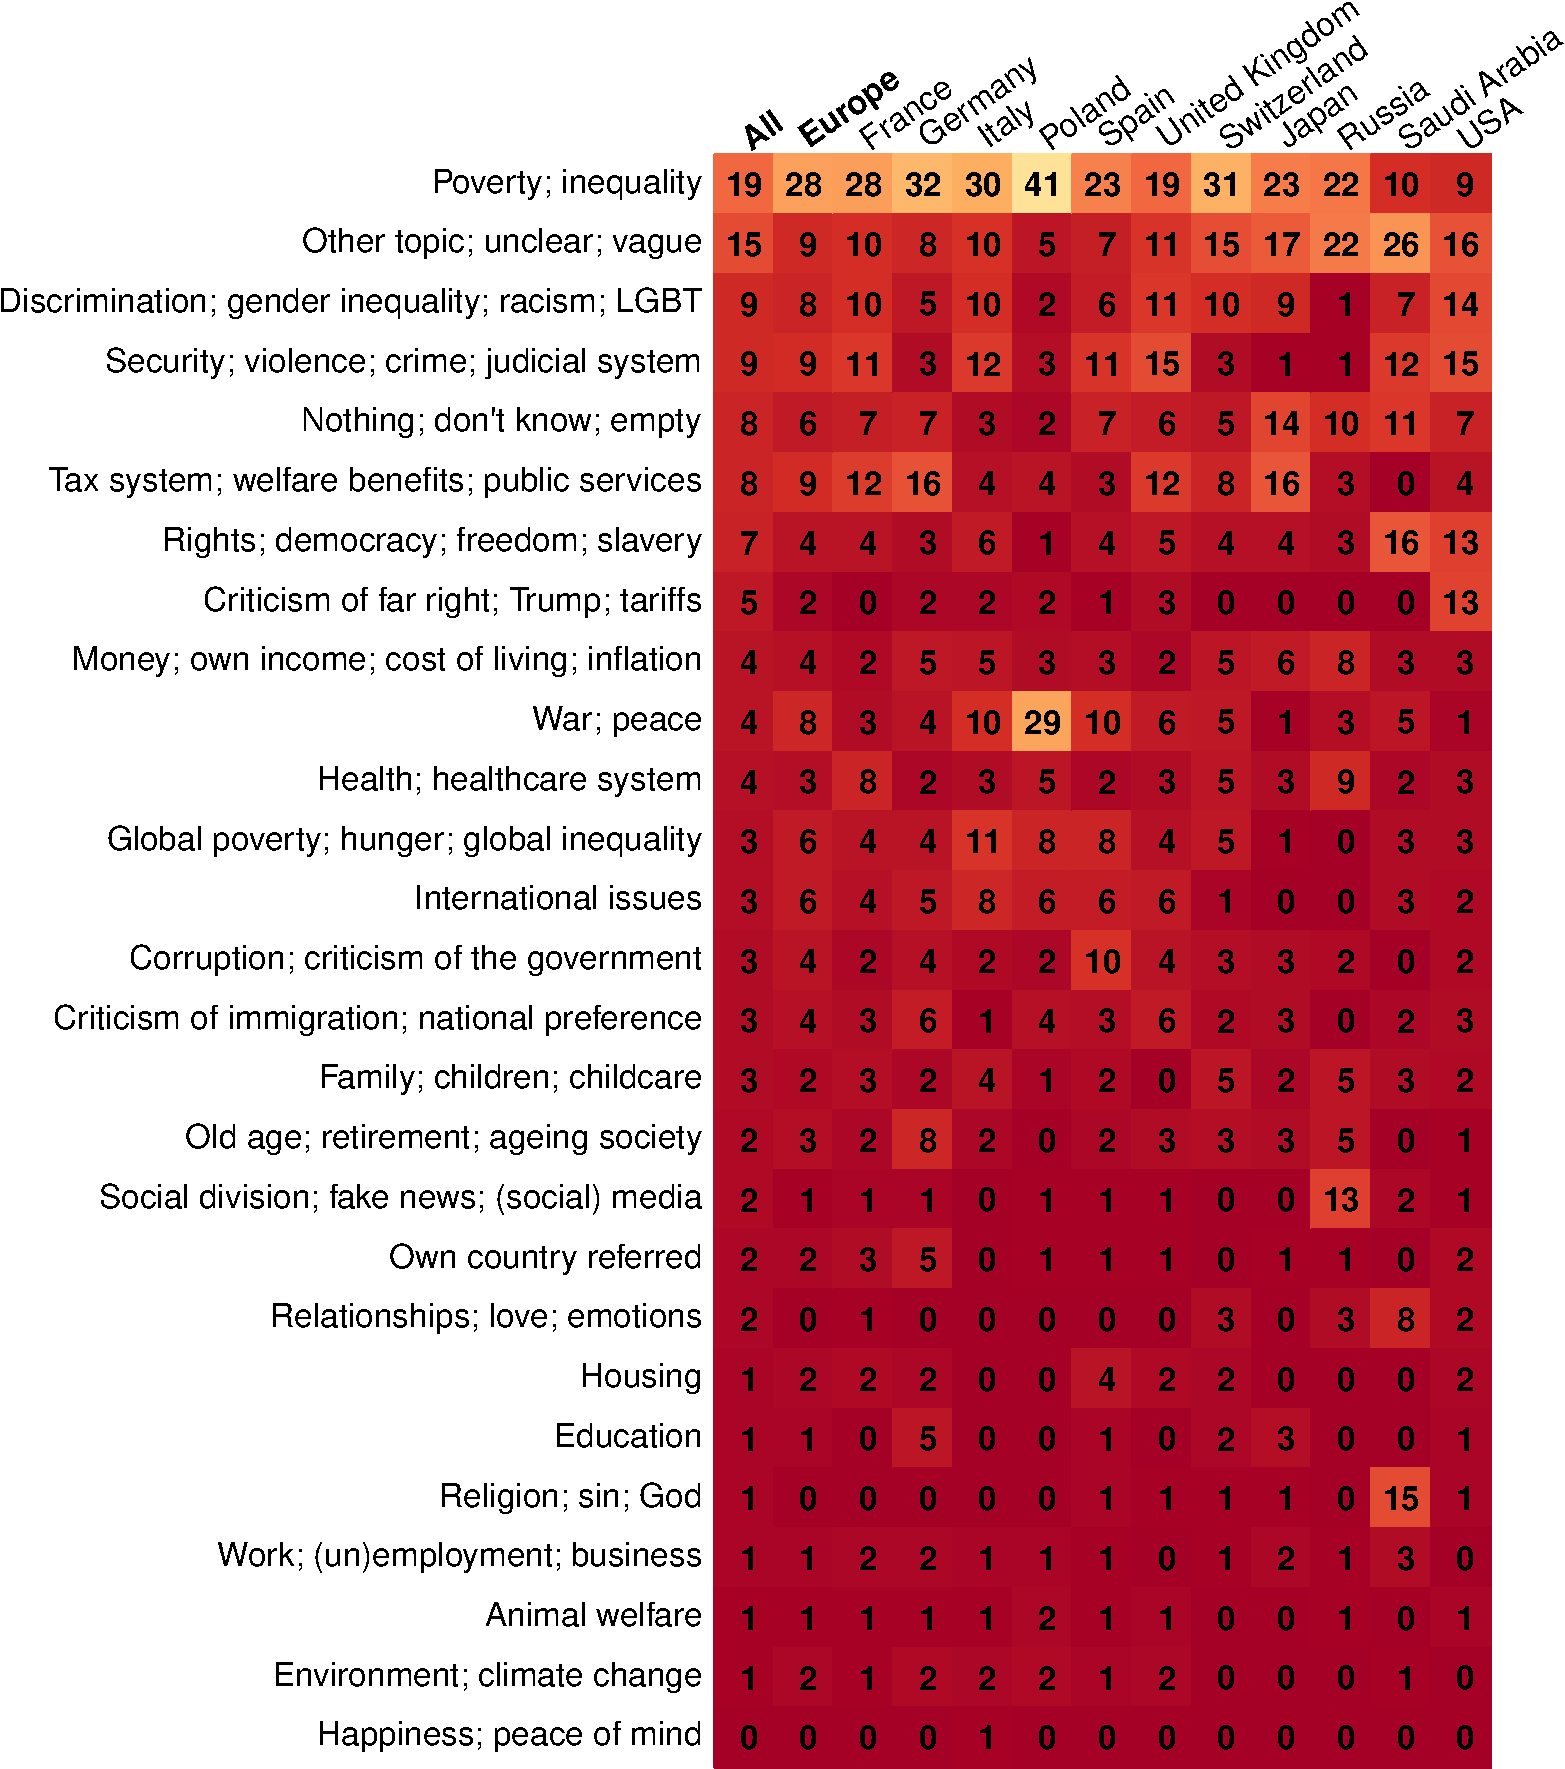
\includegraphics[height=.85\textheight]{../figures/country_comparison/field_injustice_manual_positive.pdf}} 
\end{figure}

\begin{figure}[h!]
    \caption[Manual classification of \textit{issue} fields]{Manual classification of \textit{issue} fields: ``Can you name an issue that is important to you but is neglected in the public debate?'' (Question~\ref{q:issue_field}).\hfill Back~to~Section~\ref{subsec:considerations}.
    }\label{fig:issue_field}
    \makebox[\textwidth][c]{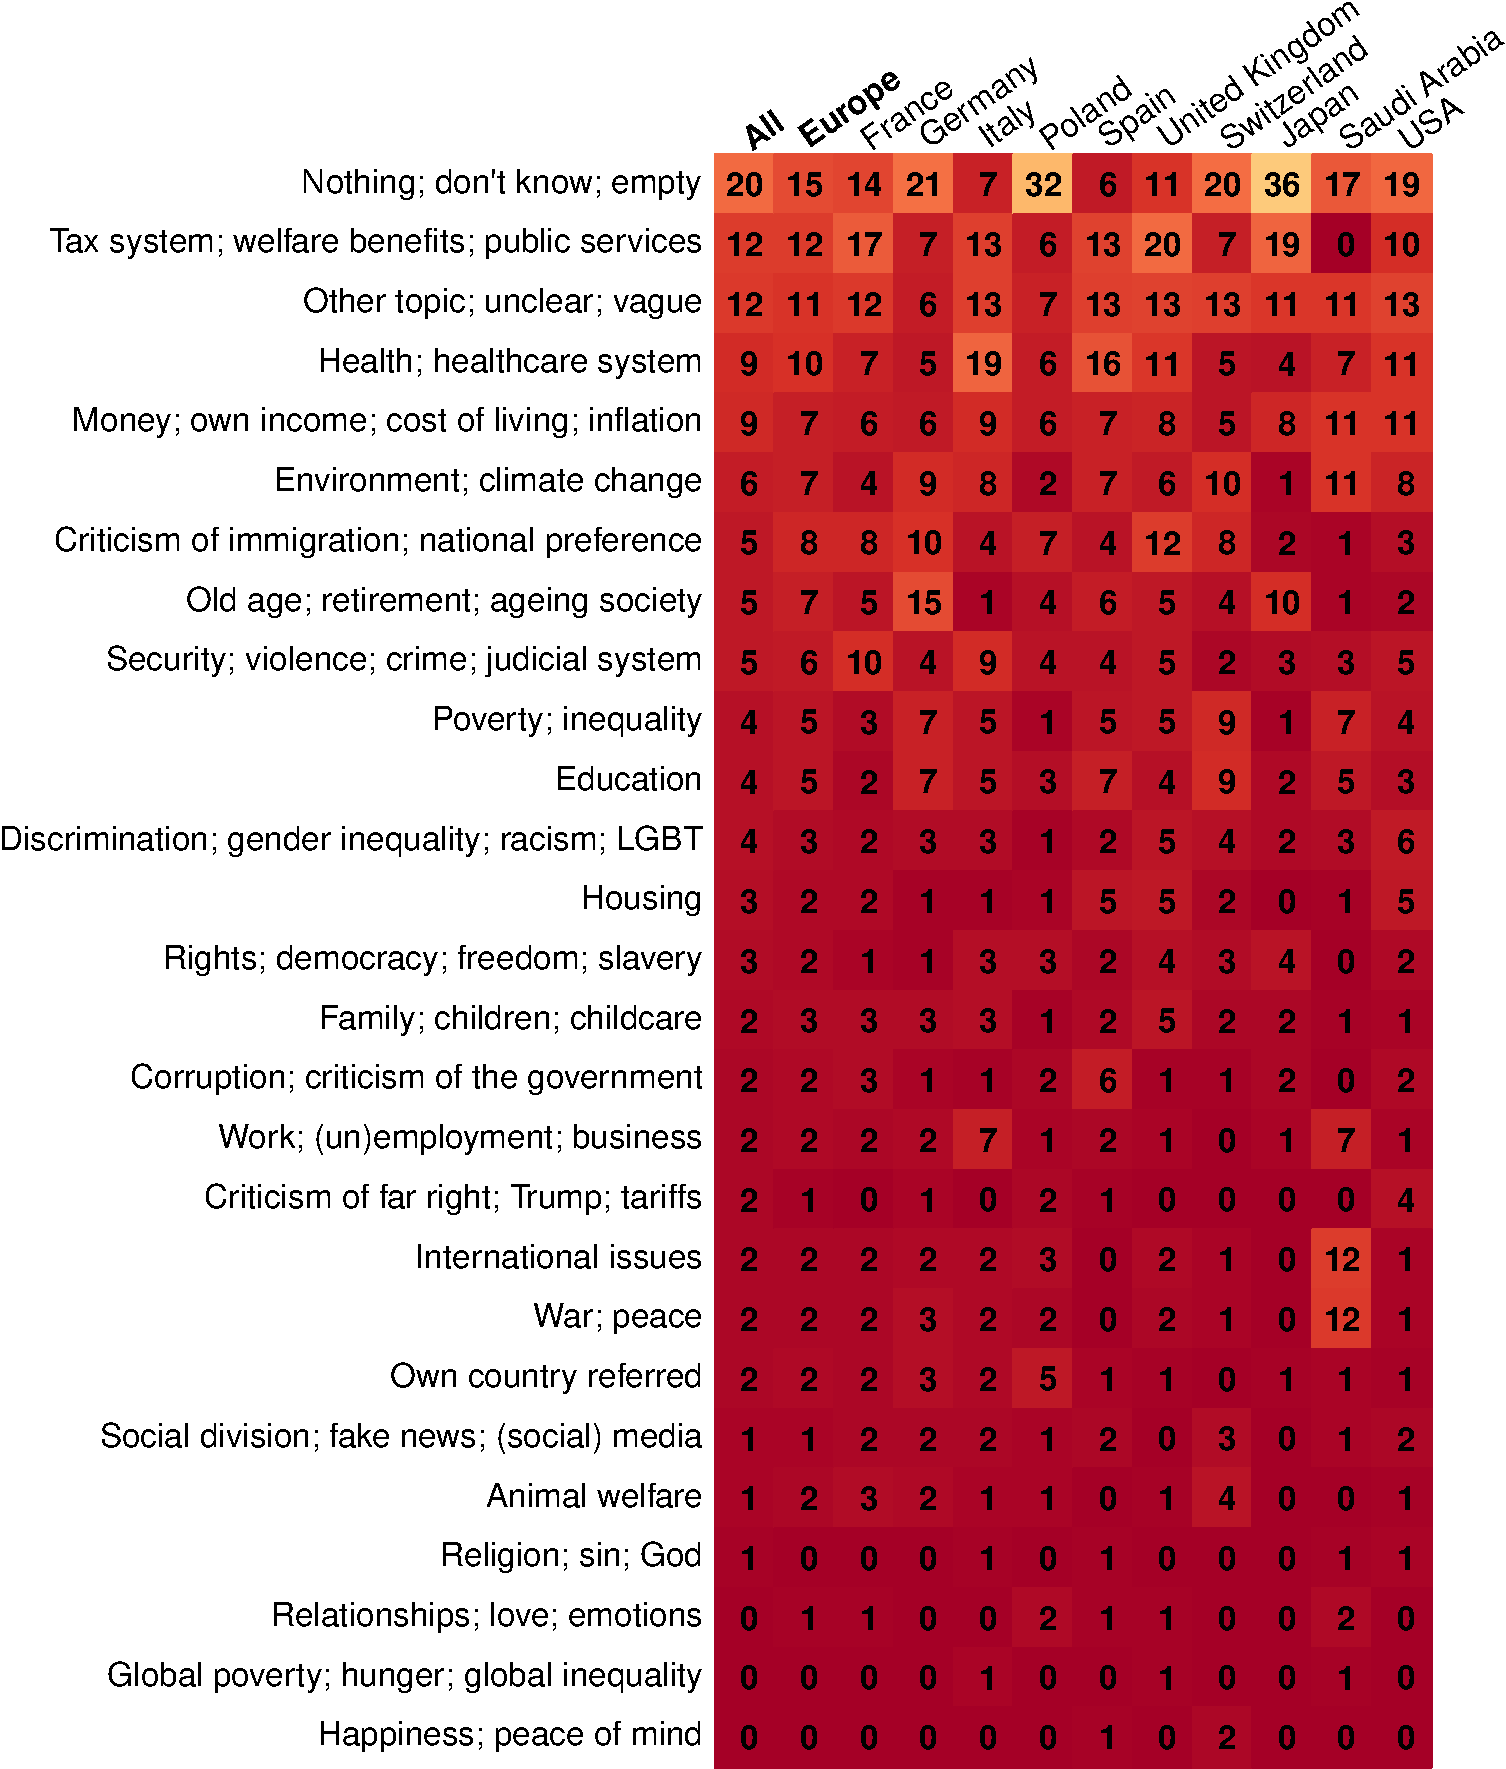
\includegraphics[height=.85\textheight]{../figures/country_comparison/field_issue_manual_positive.pdf}} 
\end{figure}

\begin{figure}
\caption[Conjoint analysis: effect of development aid and millionaire tax by vote]{Effect by vote at the last election on the likelihood that a political program is preferred of containing the following policy (compared to no foreign policy in the program). (See Figure \ref{fig:conjoint} for the simple figure). \hfill (Question~\ref{q:conjoint})} \label{fig:conjoint_vote}
\begin{subfigure}{\textwidth}
  \caption[]{Cut development aid.}
  \makebox[\textwidth][c]{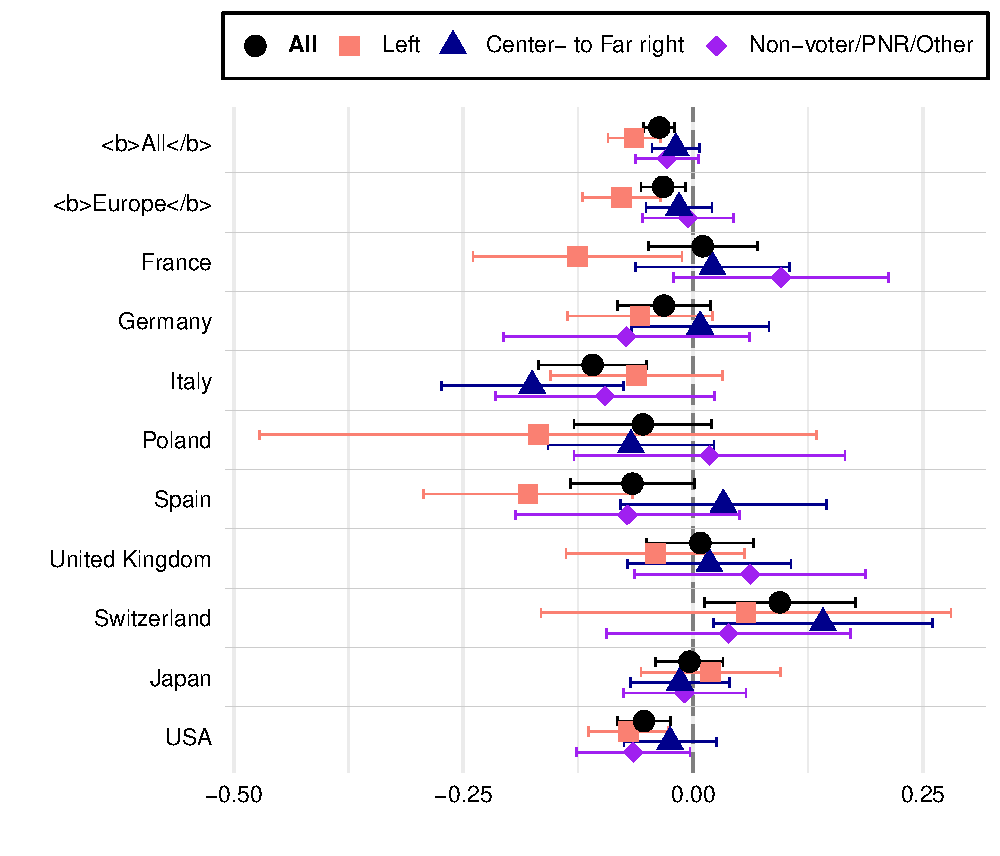
\includegraphics[width=.75\textwidth]{../figures/country_comparison/program_preferred_by_cut_aid_vote_country.pdf}}
\end{subfigure} 
\begin{subfigure}{\textwidth}
  \caption[]{Int'l tax on millionaires with 30\% financing health and education in low-income countries.}%\begin{flushright}
  \makebox[\textwidth][c]{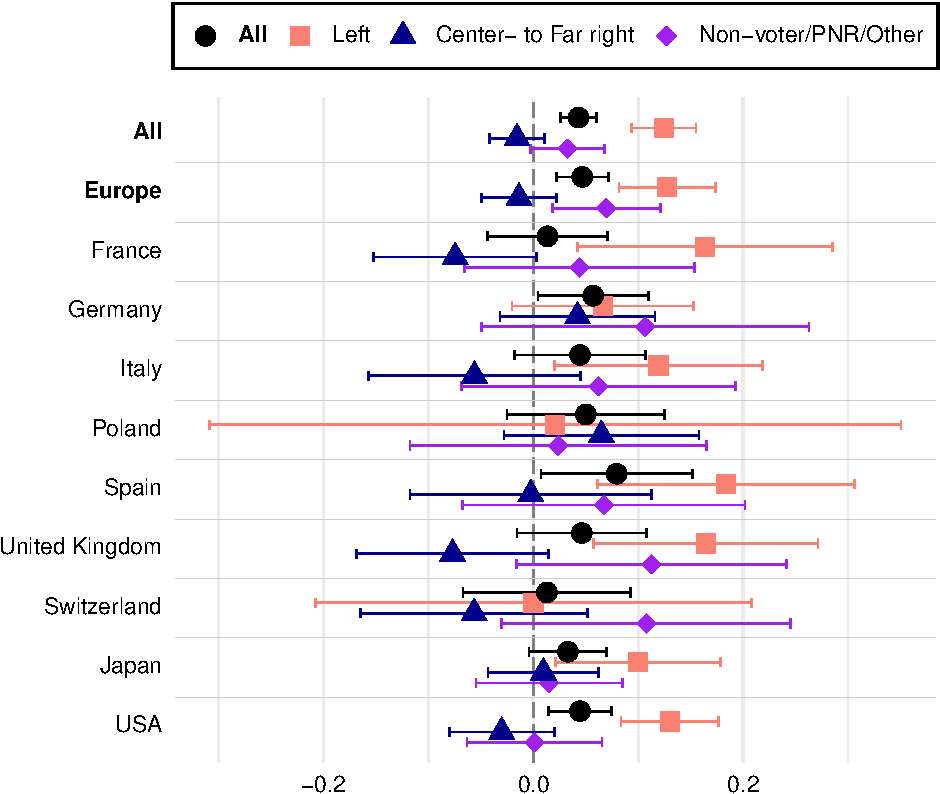
\includegraphics[width=.75\textwidth]{../figures/country_comparison/program_preferred_by_millionaire_tax_vote_country.pdf}}%\end{flushright}
\end{subfigure}
\end{figure}

\begin{figure}[h!]
    \caption[Conjoint analysis in France]{Conjoint analysis in France (Average Marginal Component Effect). Cf. Figure \ref{fig:conjoint_FR_original} for French. \hfill (Question~\ref{q:conjoint}).
    }\label{fig:conjoint_FR}
    \makebox[\textwidth][c]{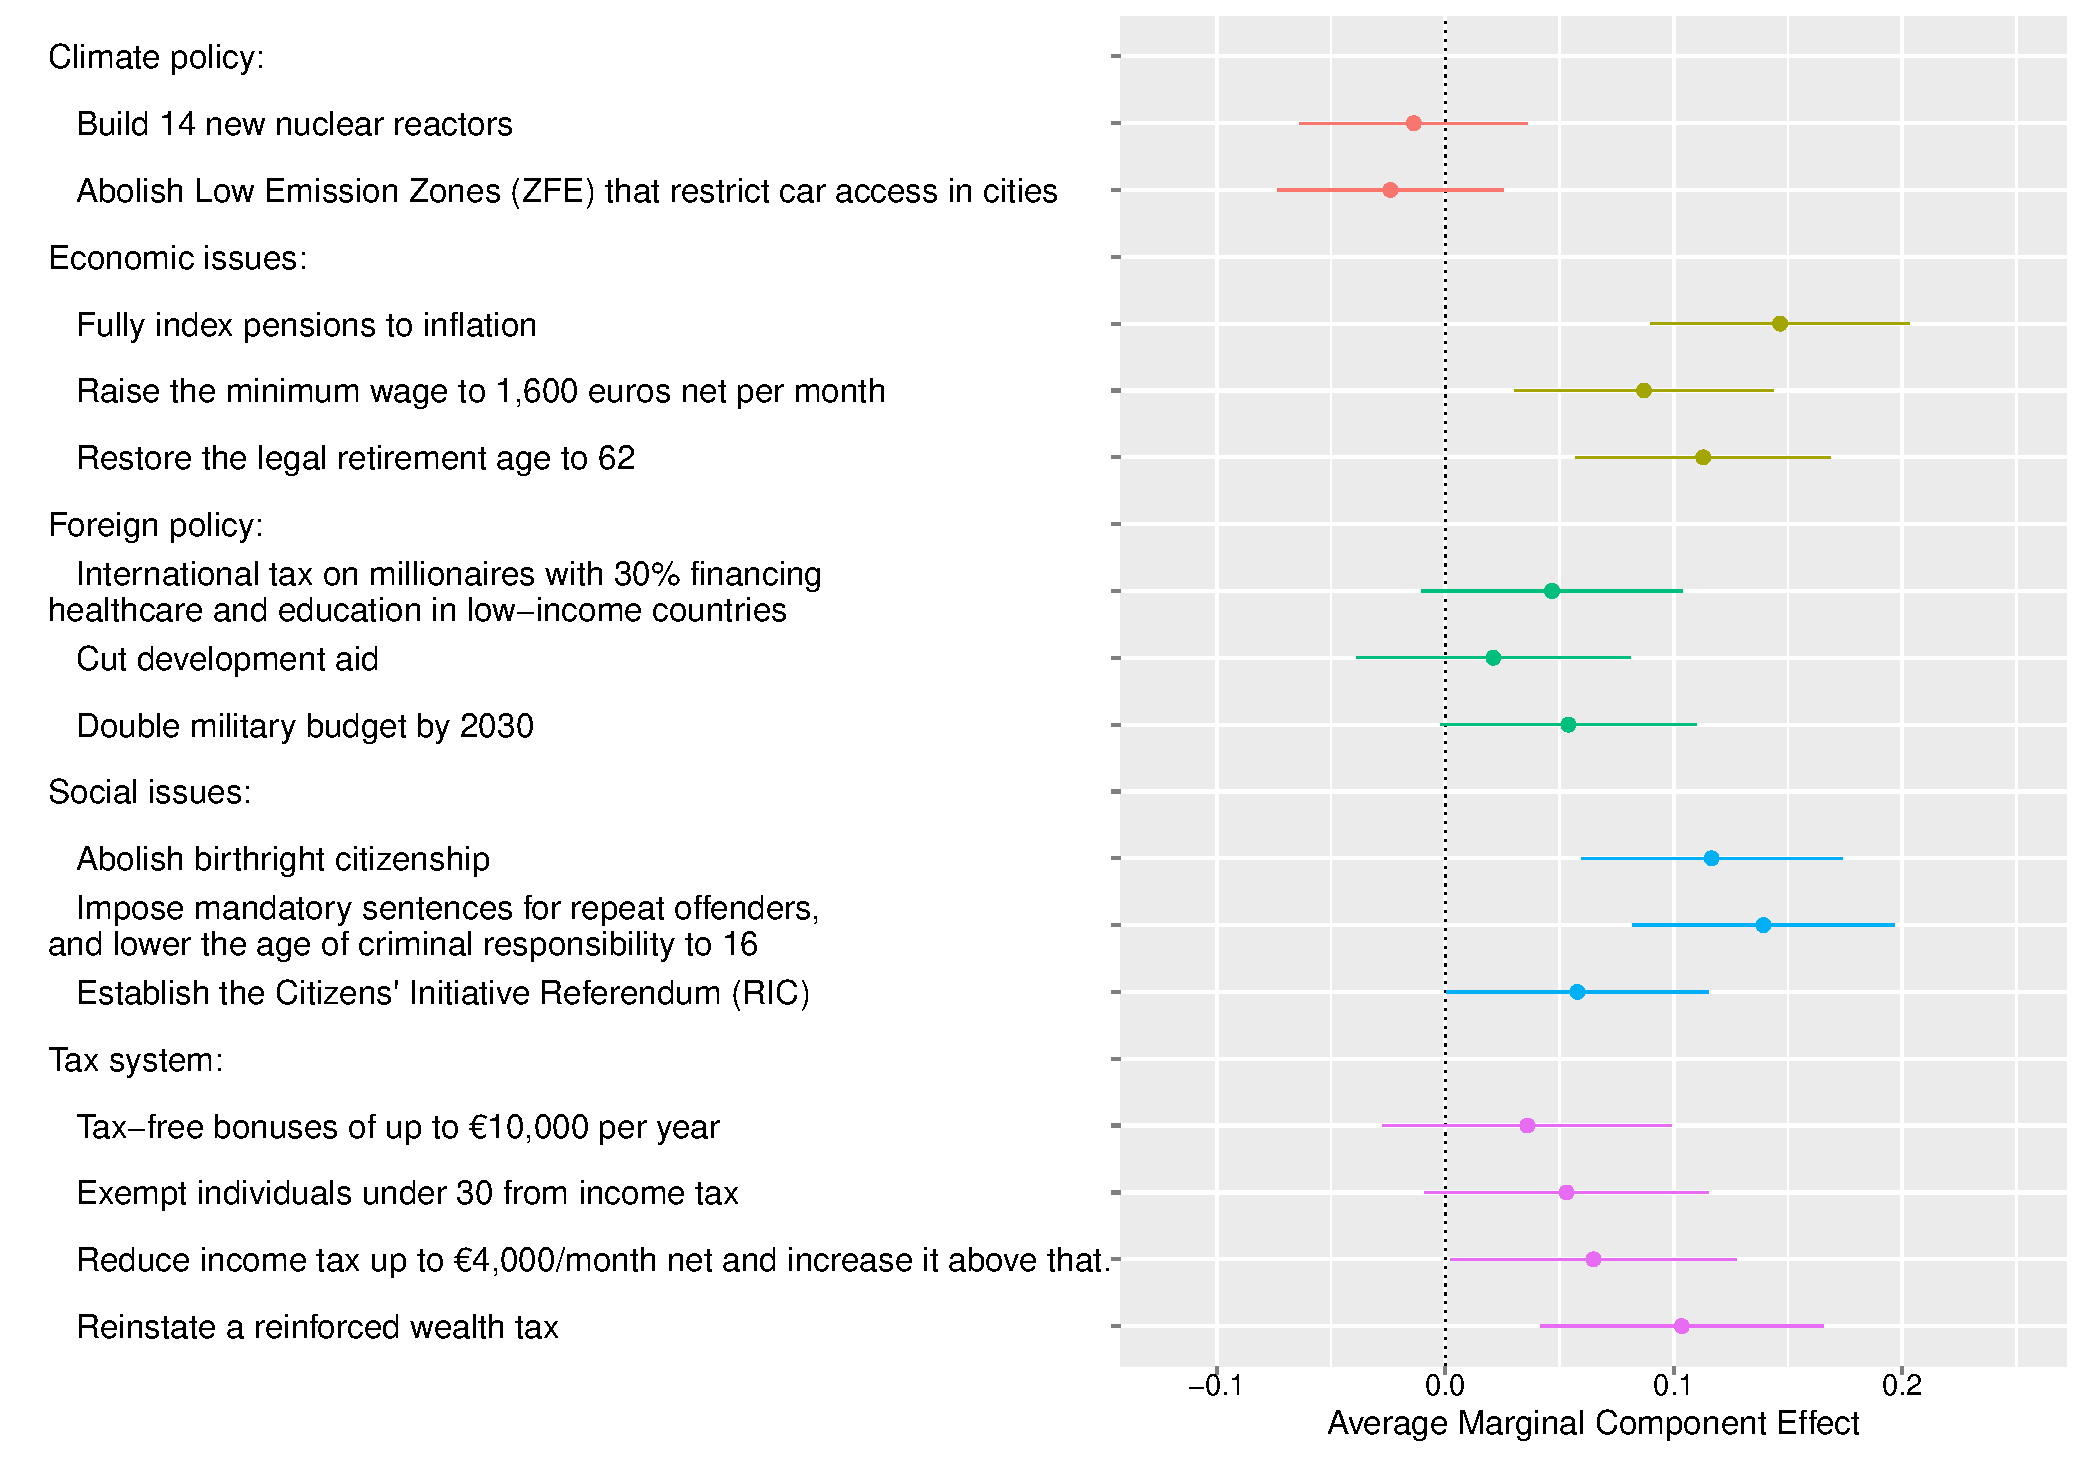
\includegraphics[width=\textwidth]{../figures/all/conjoint_EN-FR.pdf}} 
\end{figure}

\begin{figure}[h!]
    \caption[Conjoint analysis in Germany]{Conjoint analysis in Germany (Average Marginal Component Effect). Cf. Figure \ref{fig:conjoint_DE_original} for German. \hfill (Question~\ref{q:conjoint}).
    }\label{fig:conjoint_DE}
    \makebox[\textwidth][c]{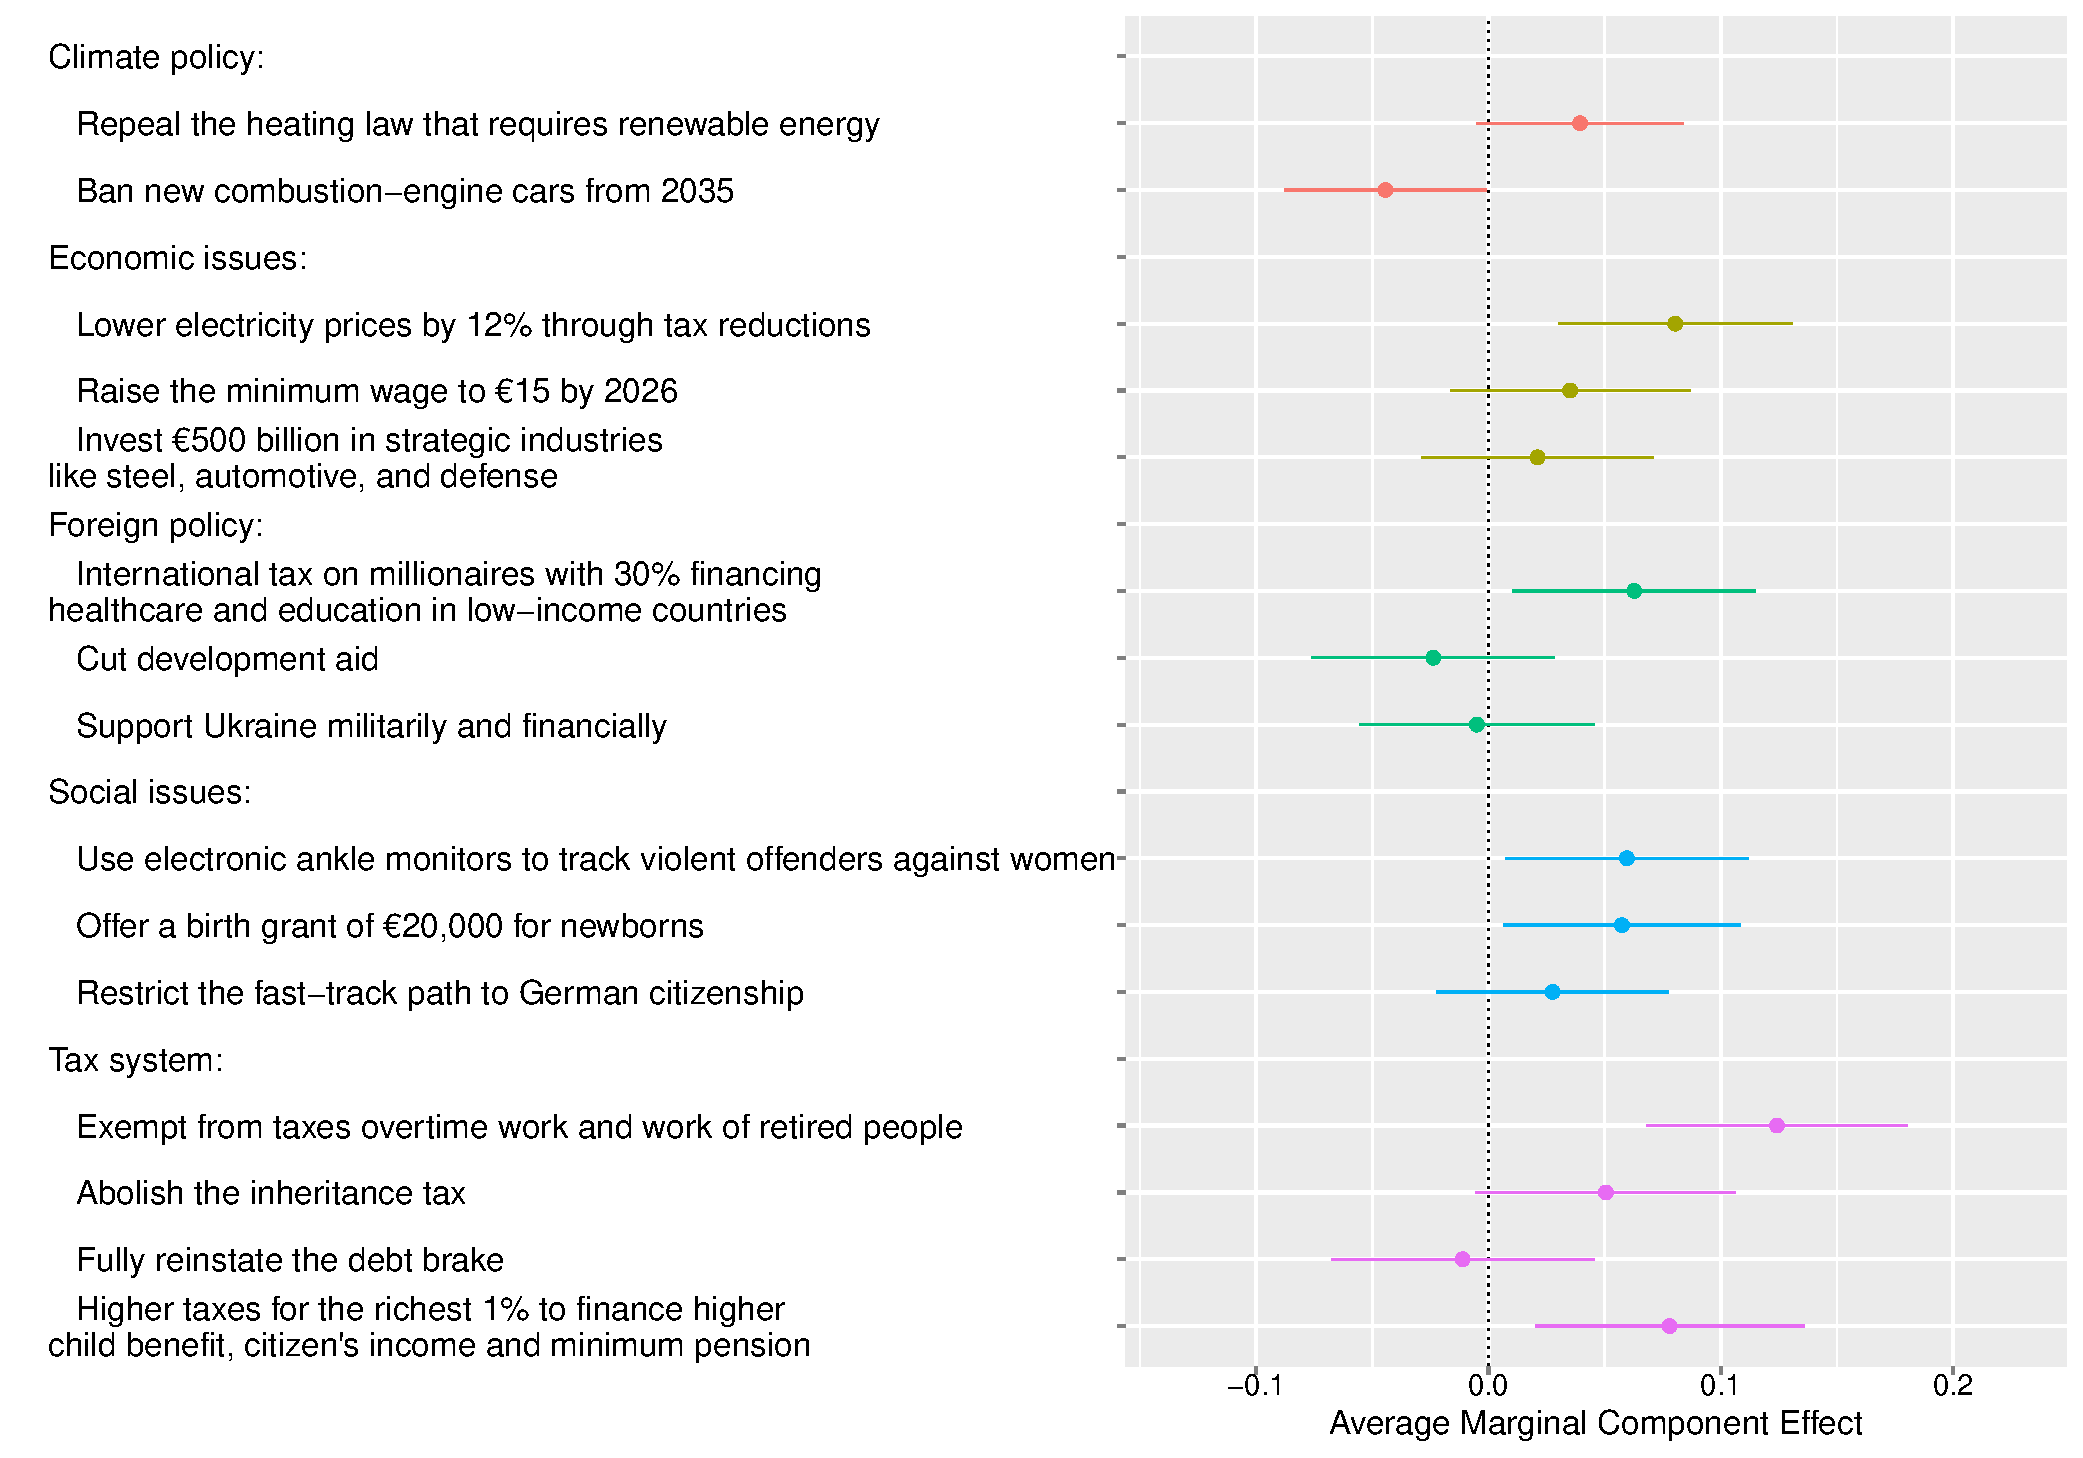
\includegraphics[width=\textwidth]{../figures/all/conjoint_EN-DE.pdf}} 
\end{figure}

\begin{figure}[h!]
    \caption[Conjoint analysis in Italy]{Conjoint analysis in Italy (Average Marginal Component Effect). Cf. Figure \ref{fig:conjoint_IT_original} for Italian. \hfill (Question~\ref{q:conjoint}).
    }\label{fig:conjoint_IT}
    \makebox[\textwidth][c]{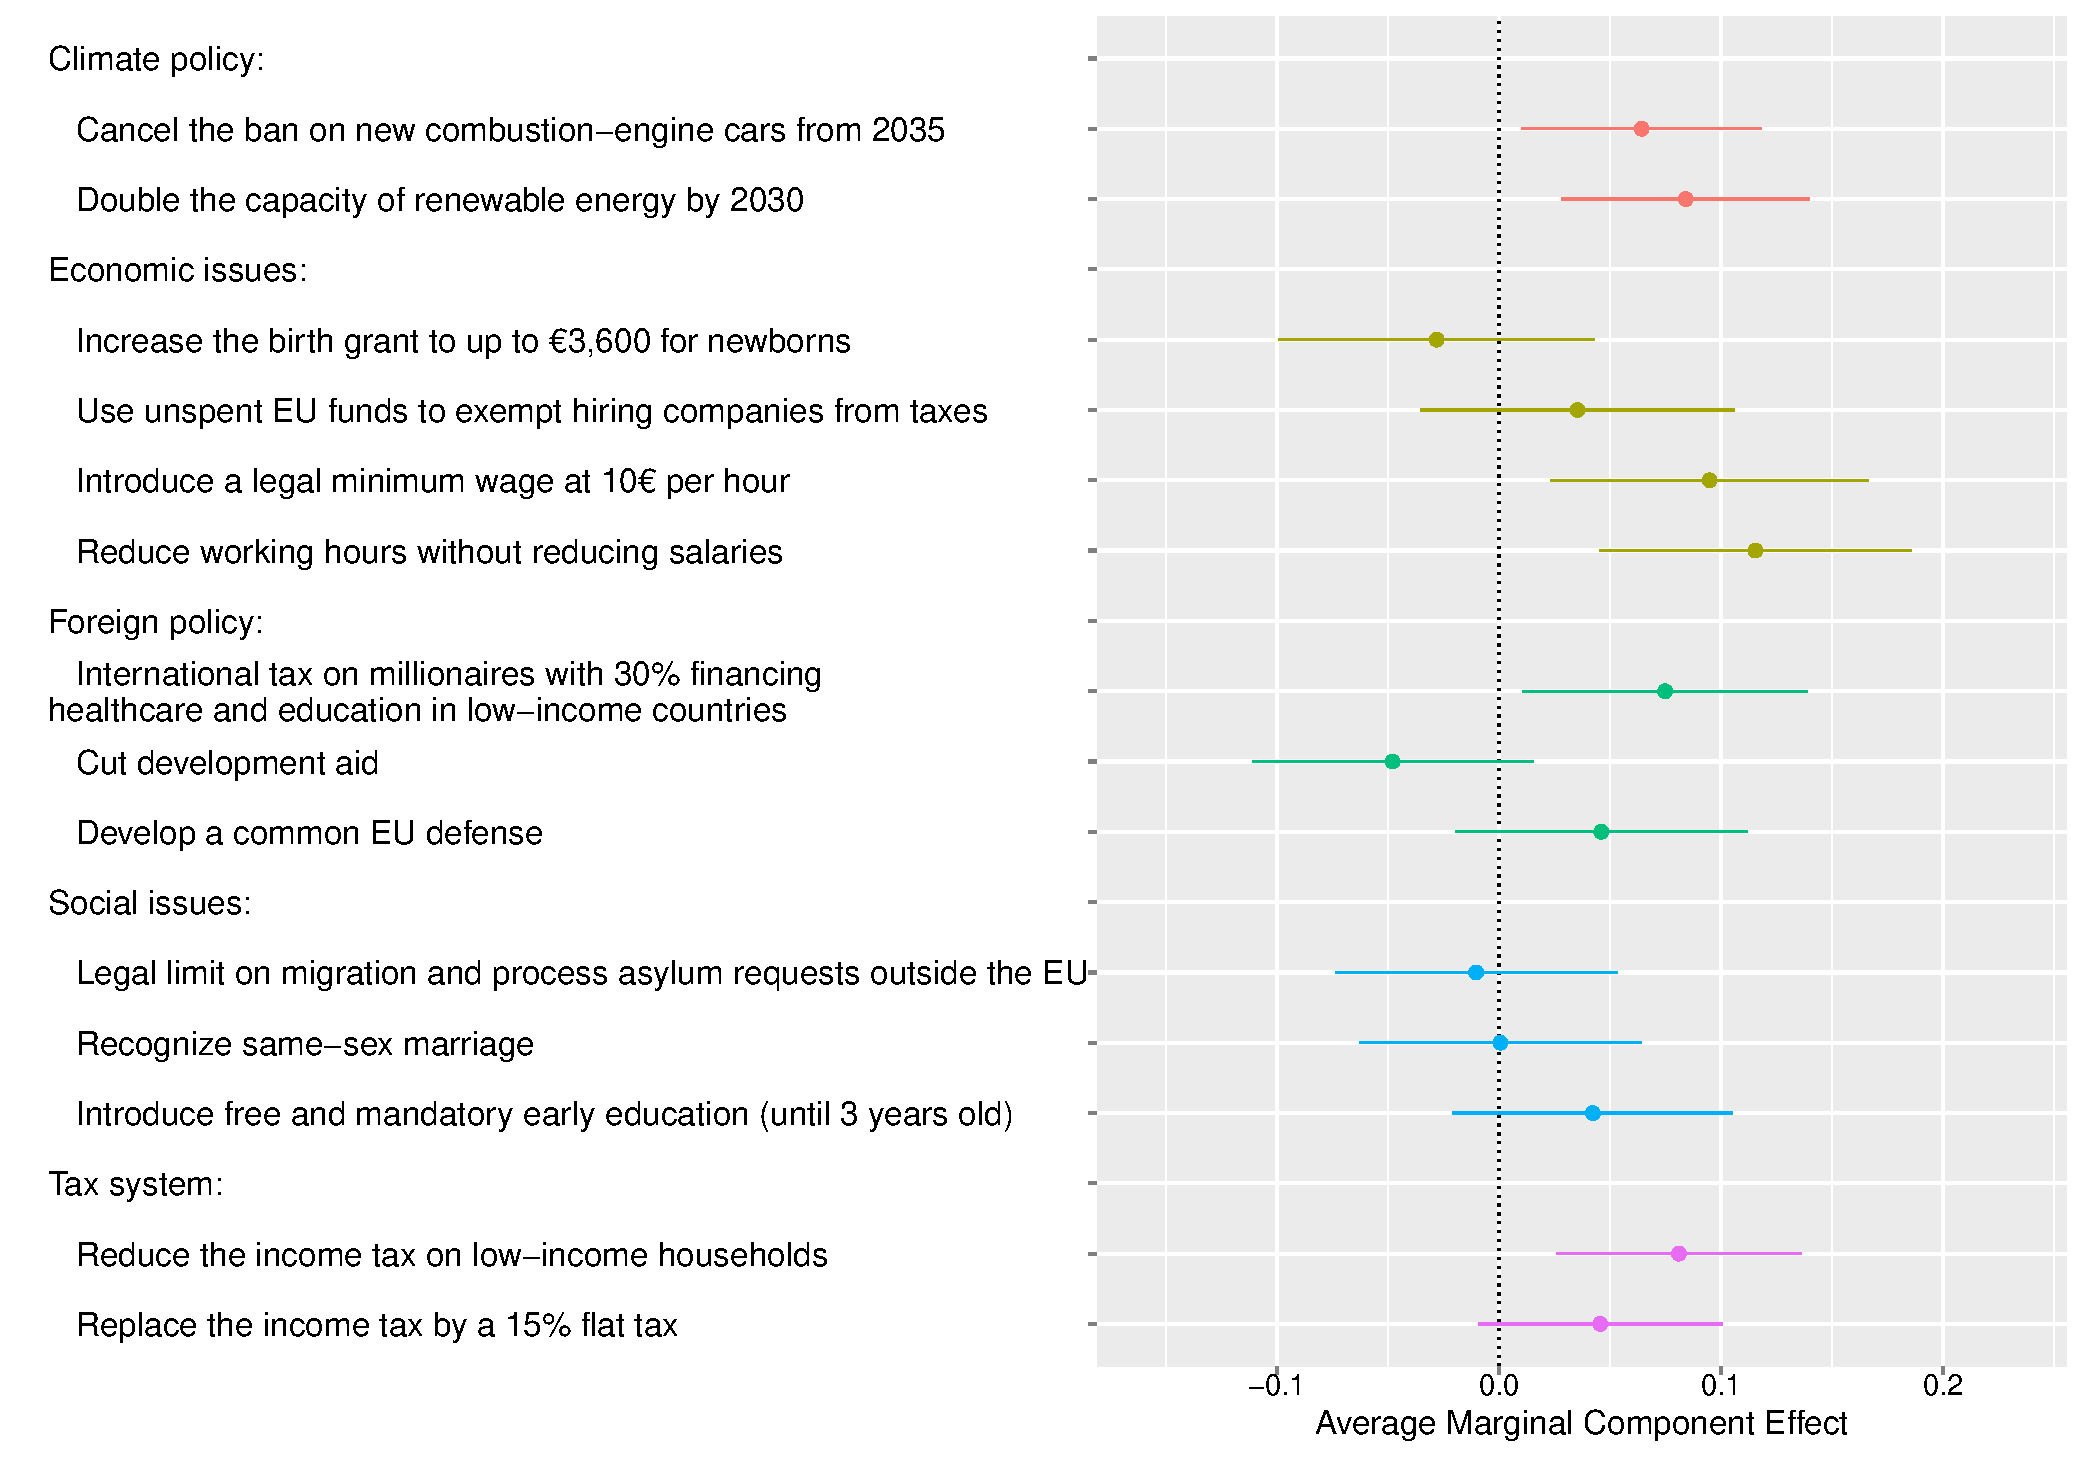
\includegraphics[width=\textwidth]{../figures/all/conjoint_EN-IT.pdf}} 
\end{figure}

\begin{figure}[h!]
    \caption[Conjoint analysis in Poland]{Conjoint analysis in Poland (Average Marginal Component Effect). Cf. Figure \ref{fig:conjoint_PL_original} for Polish. \hfill (Question~\ref{q:conjoint}).
    }\label{fig:conjoint_PL}
    \makebox[\textwidth][c]{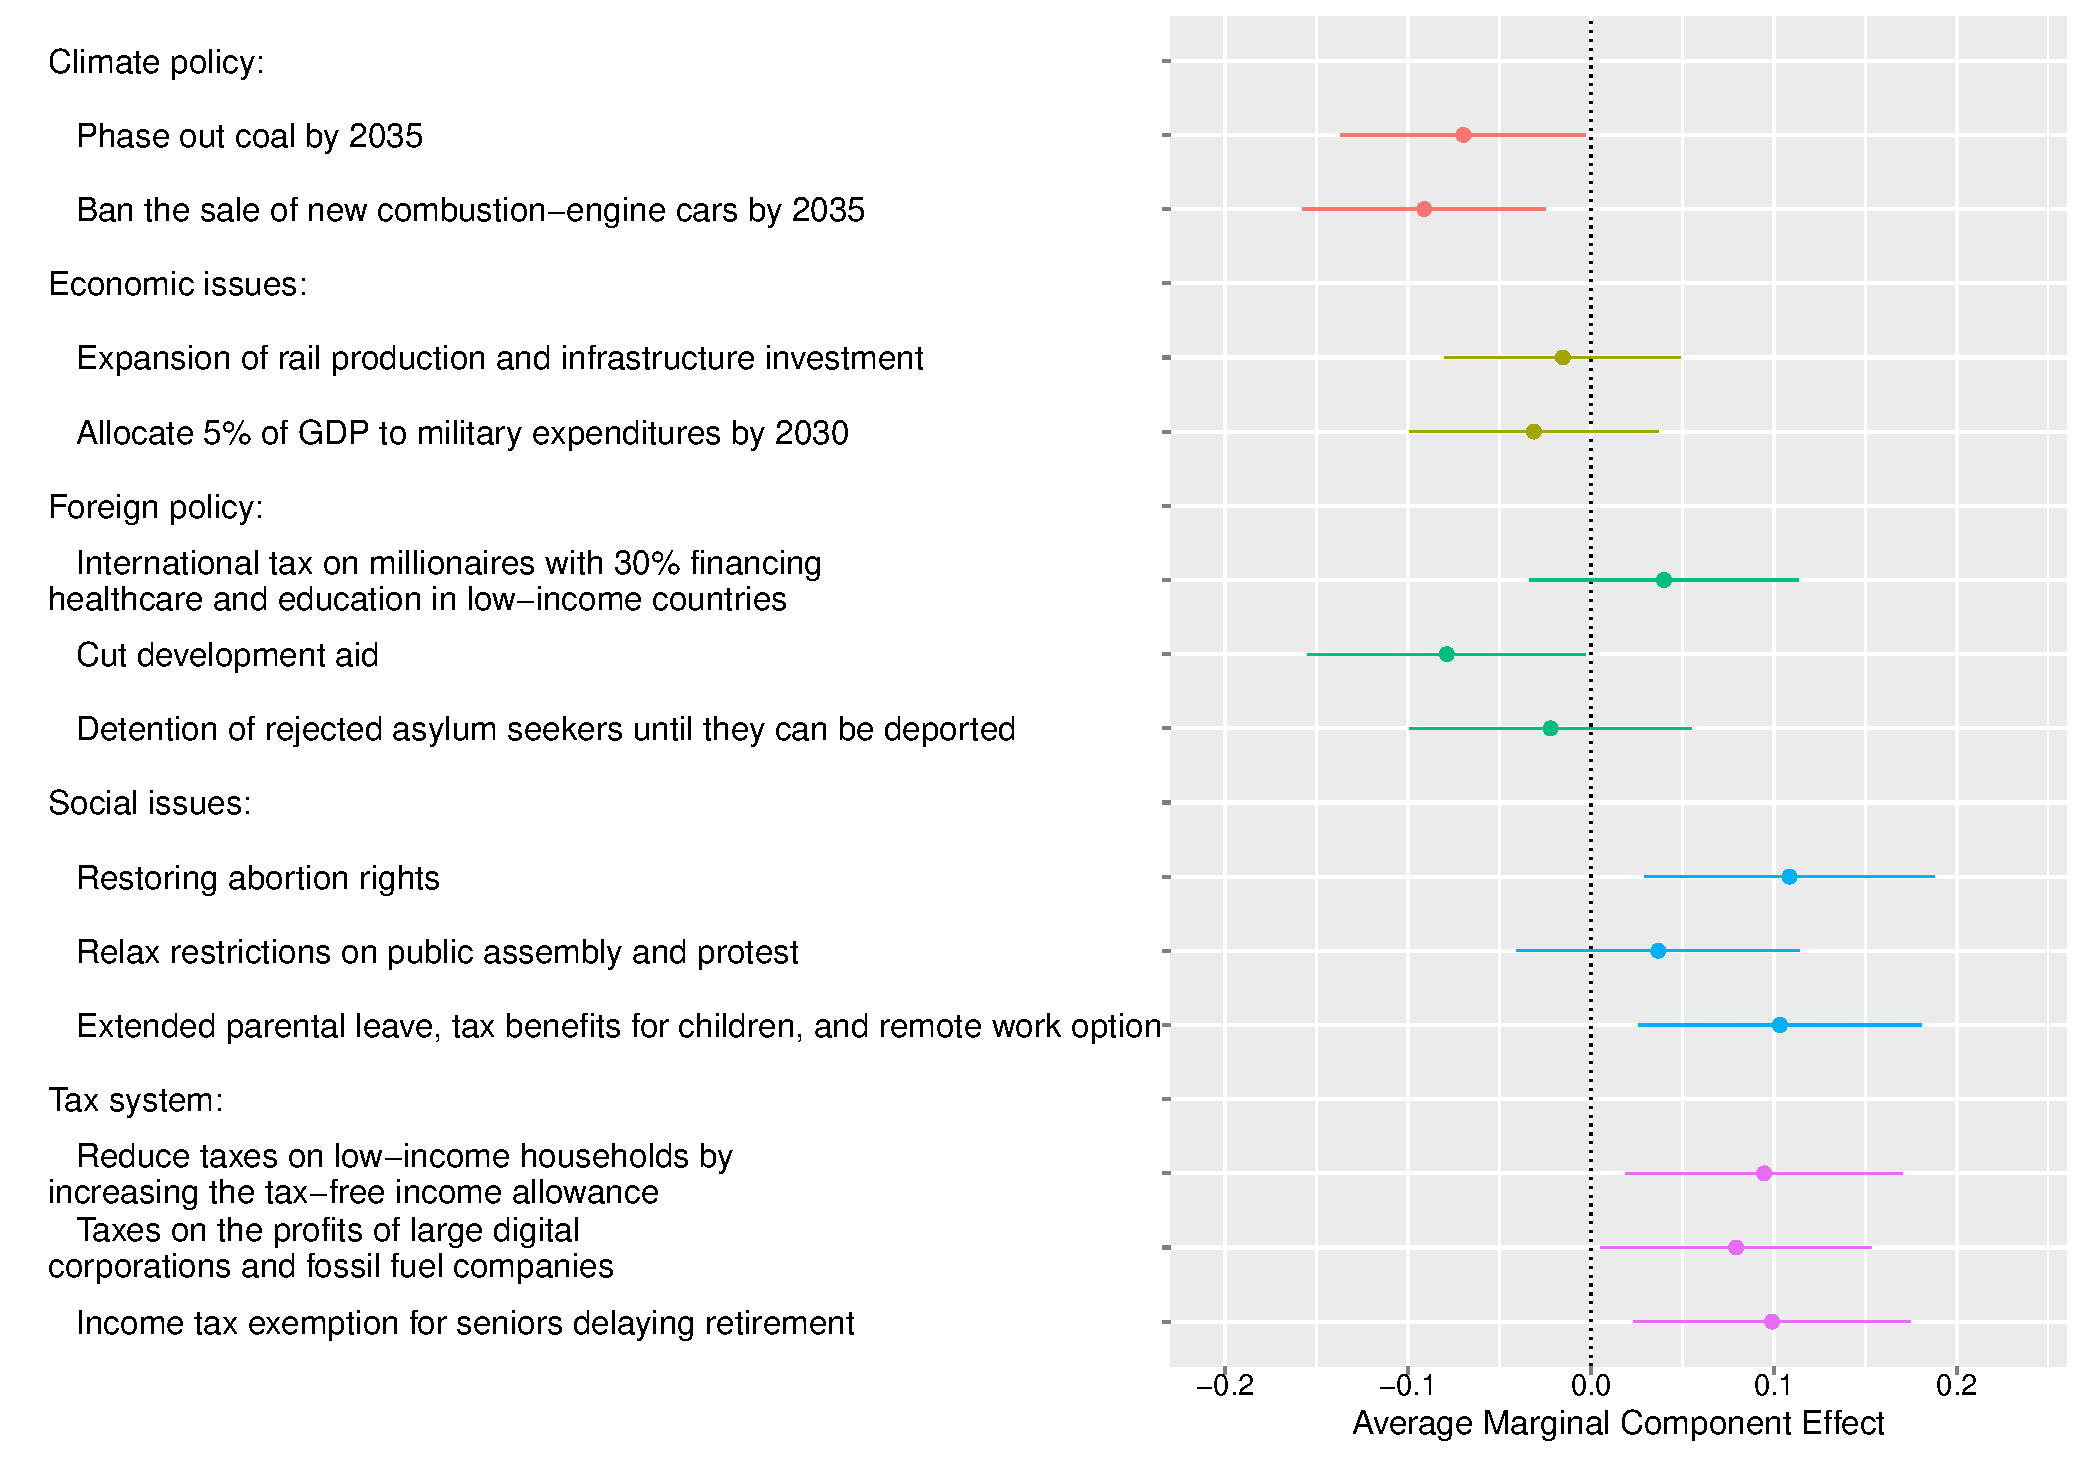
\includegraphics[width=\textwidth]{../figures/all/conjoint_EN-PL.pdf}} 
\end{figure}

\begin{figure}[h!]
    \caption[Conjoint analysis in Spain]{Conjoint analysis in Spain (Average Marginal Component Effect). Cf. Figure \ref{fig:conjoint_ES_original} for Spanish. \hfill (Question~\ref{q:conjoint}).
    }\label{fig:conjoint_ES}
    \makebox[\textwidth][c]{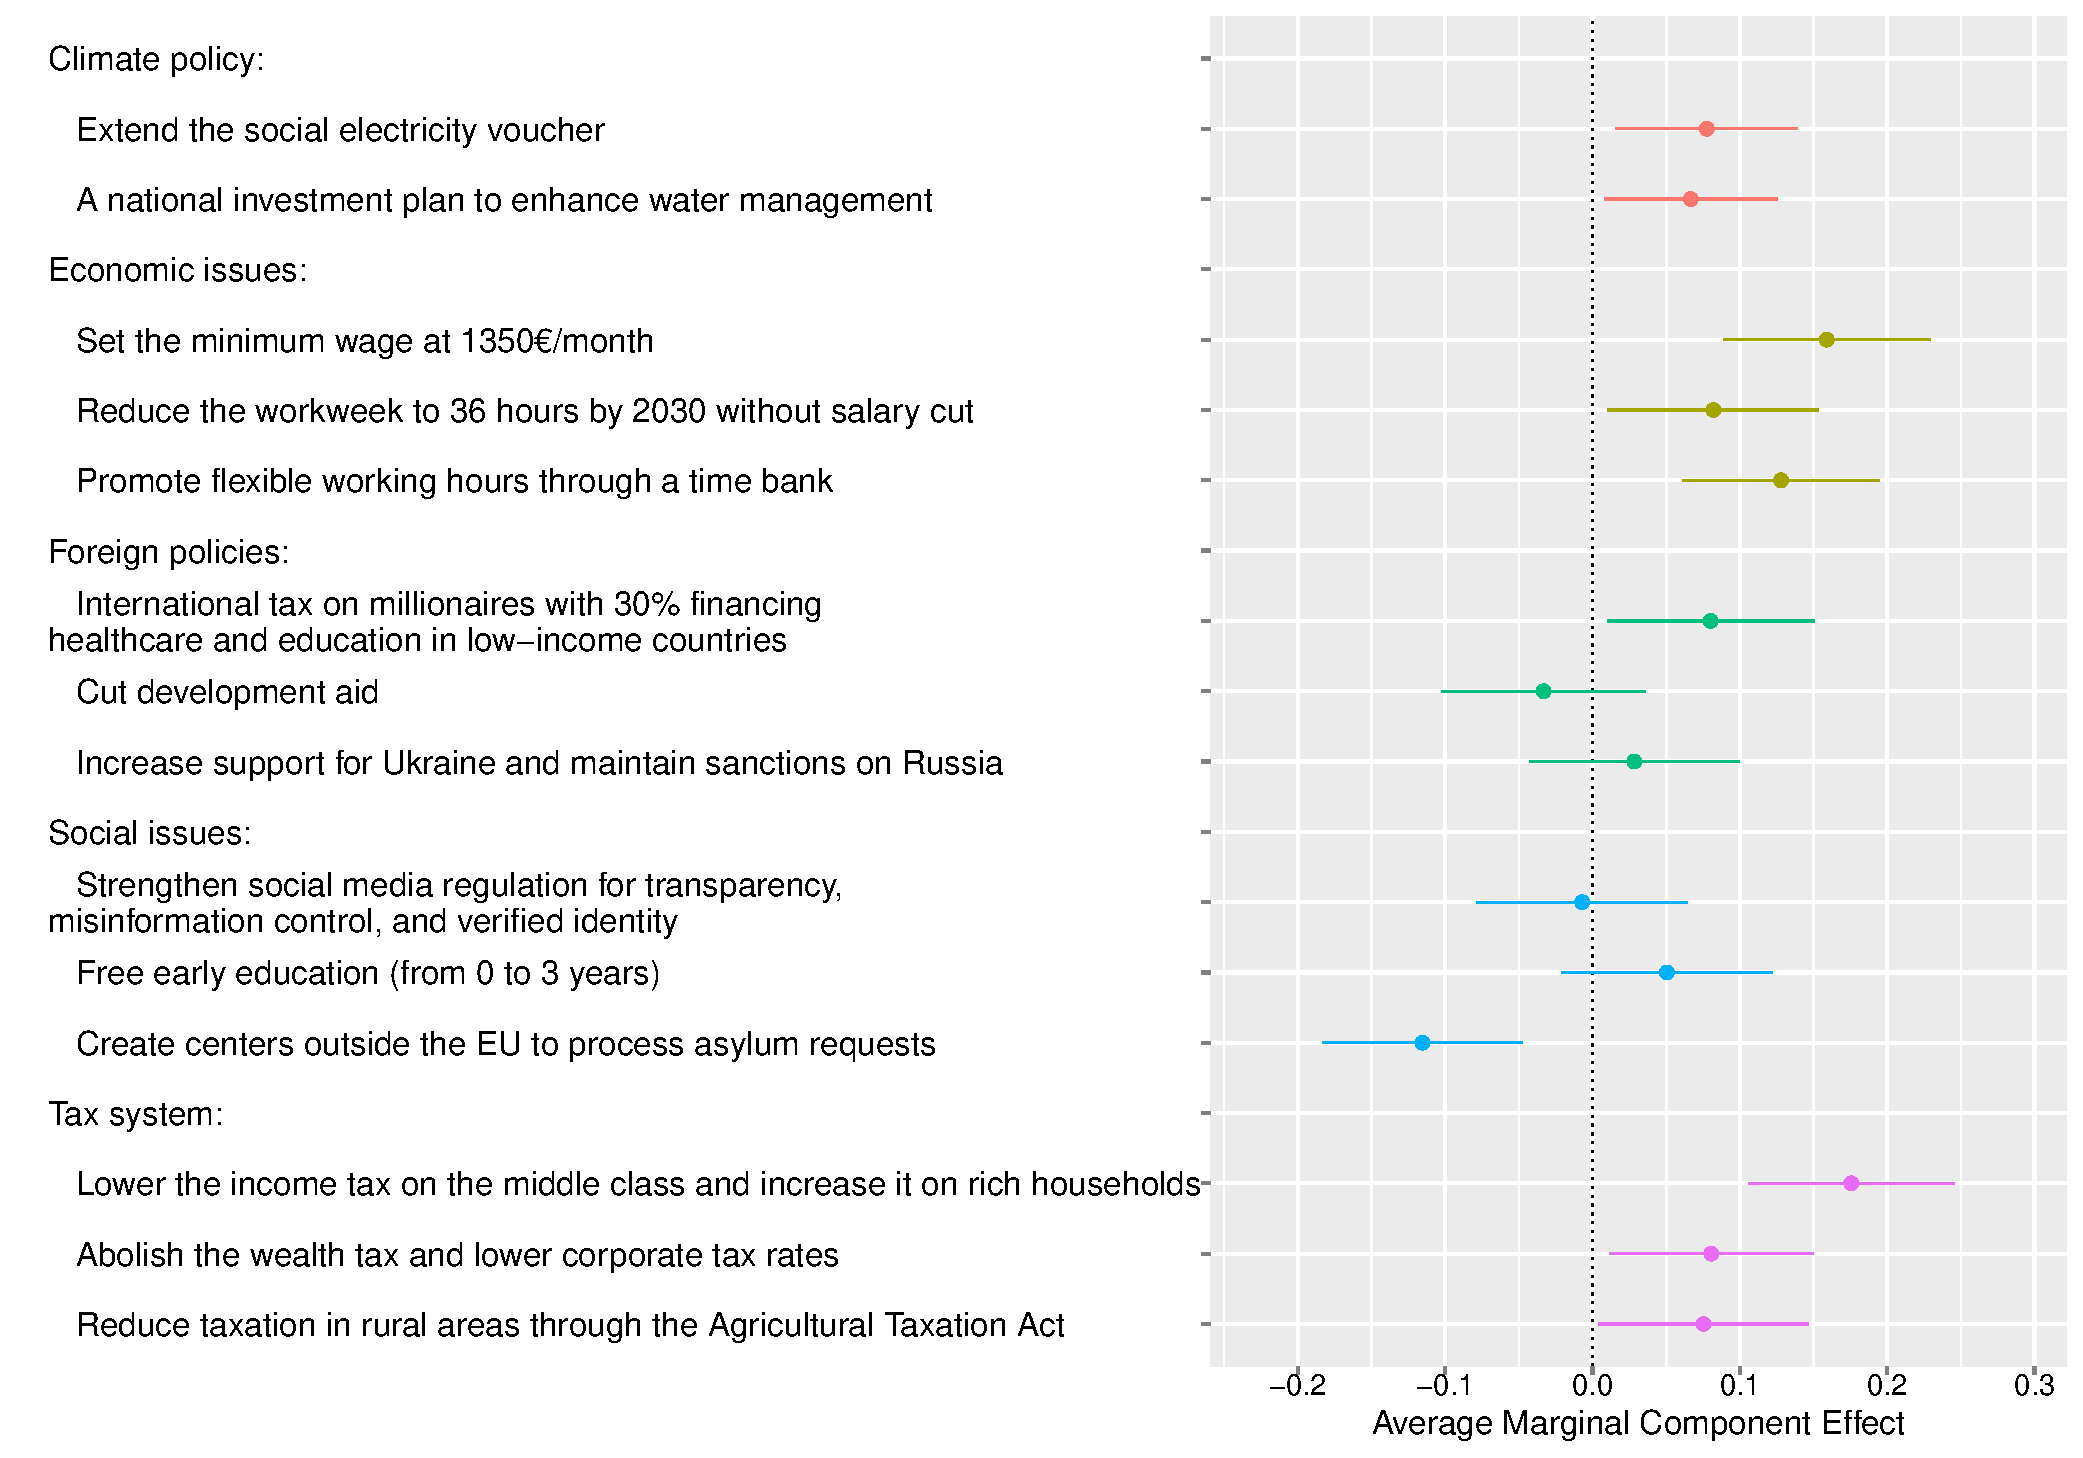
\includegraphics[width=\textwidth]{../figures/all/conjoint_EN-ES.pdf}} 
\end{figure}

\begin{figure}[h!]
    \caption[Conjoint analysis in the UK]{Conjoint analysis in the UK (Average Marginal Component Effect). \hfill (Question~\ref{q:conjoint}).
    }\label{fig:conjoint_GB}
    \makebox[\textwidth][c]{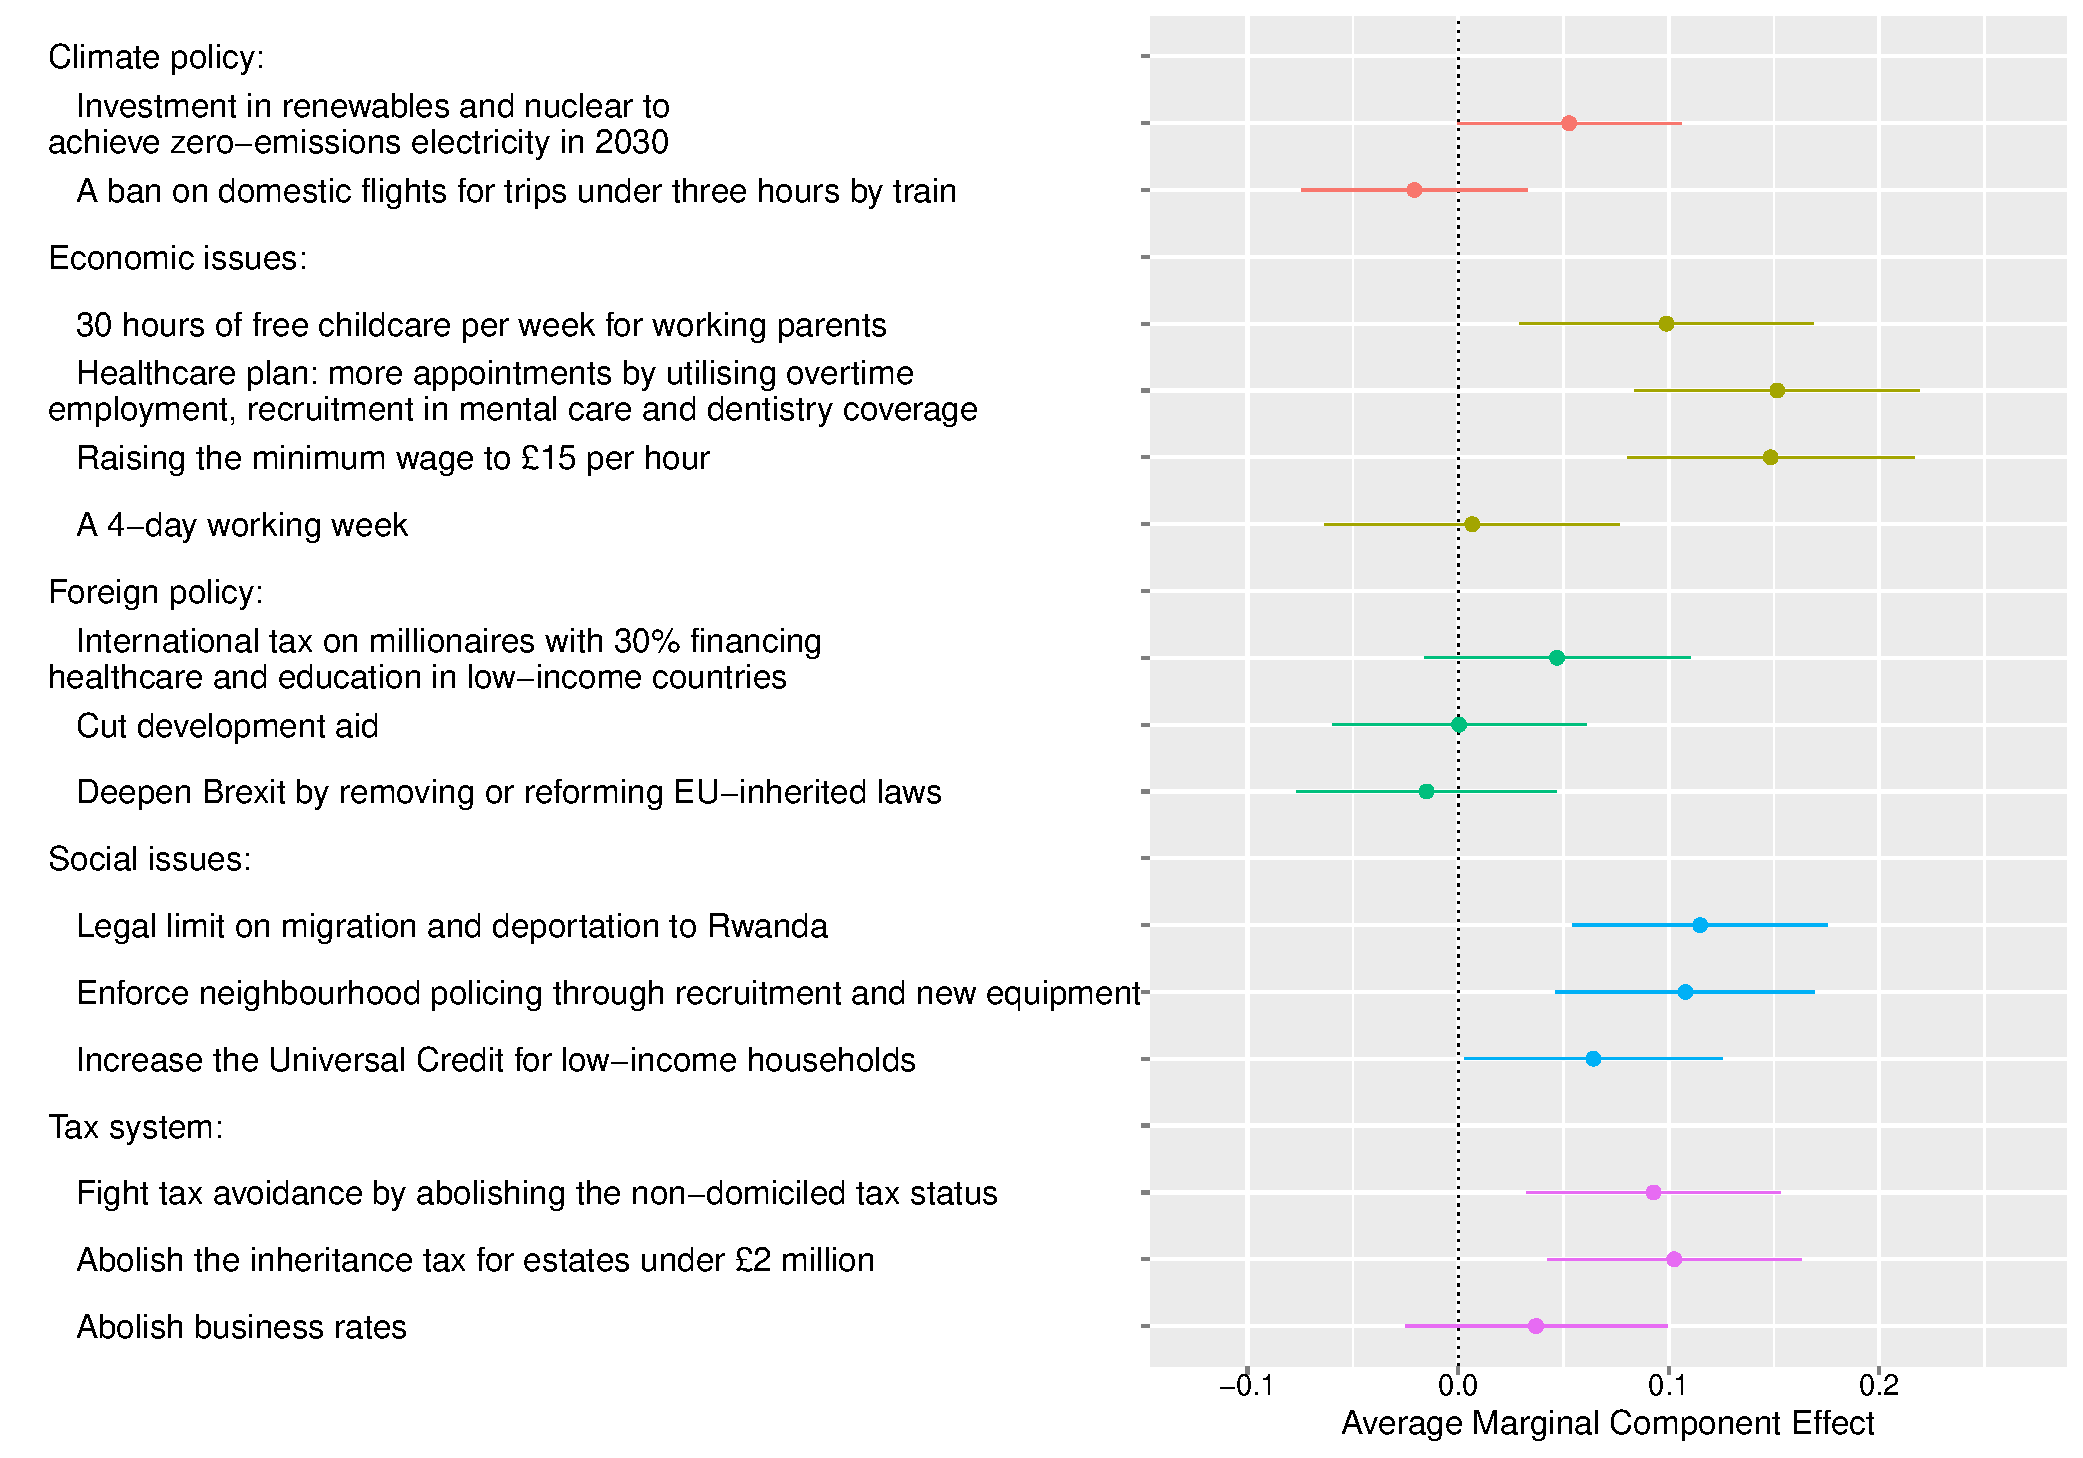
\includegraphics[width=\textwidth]{../figures/all/conjoint_EN-GB.pdf}} 
\end{figure}

\begin{figure}[h!]
    \caption[Conjoint analysis in Switzerland]{Conjoint analysis in Switzerland (Average Marginal Component Effect). \hfill (Question~\ref{q:conjoint}).
    }\label{fig:conjoint_CH}
    \makebox[\textwidth][c]{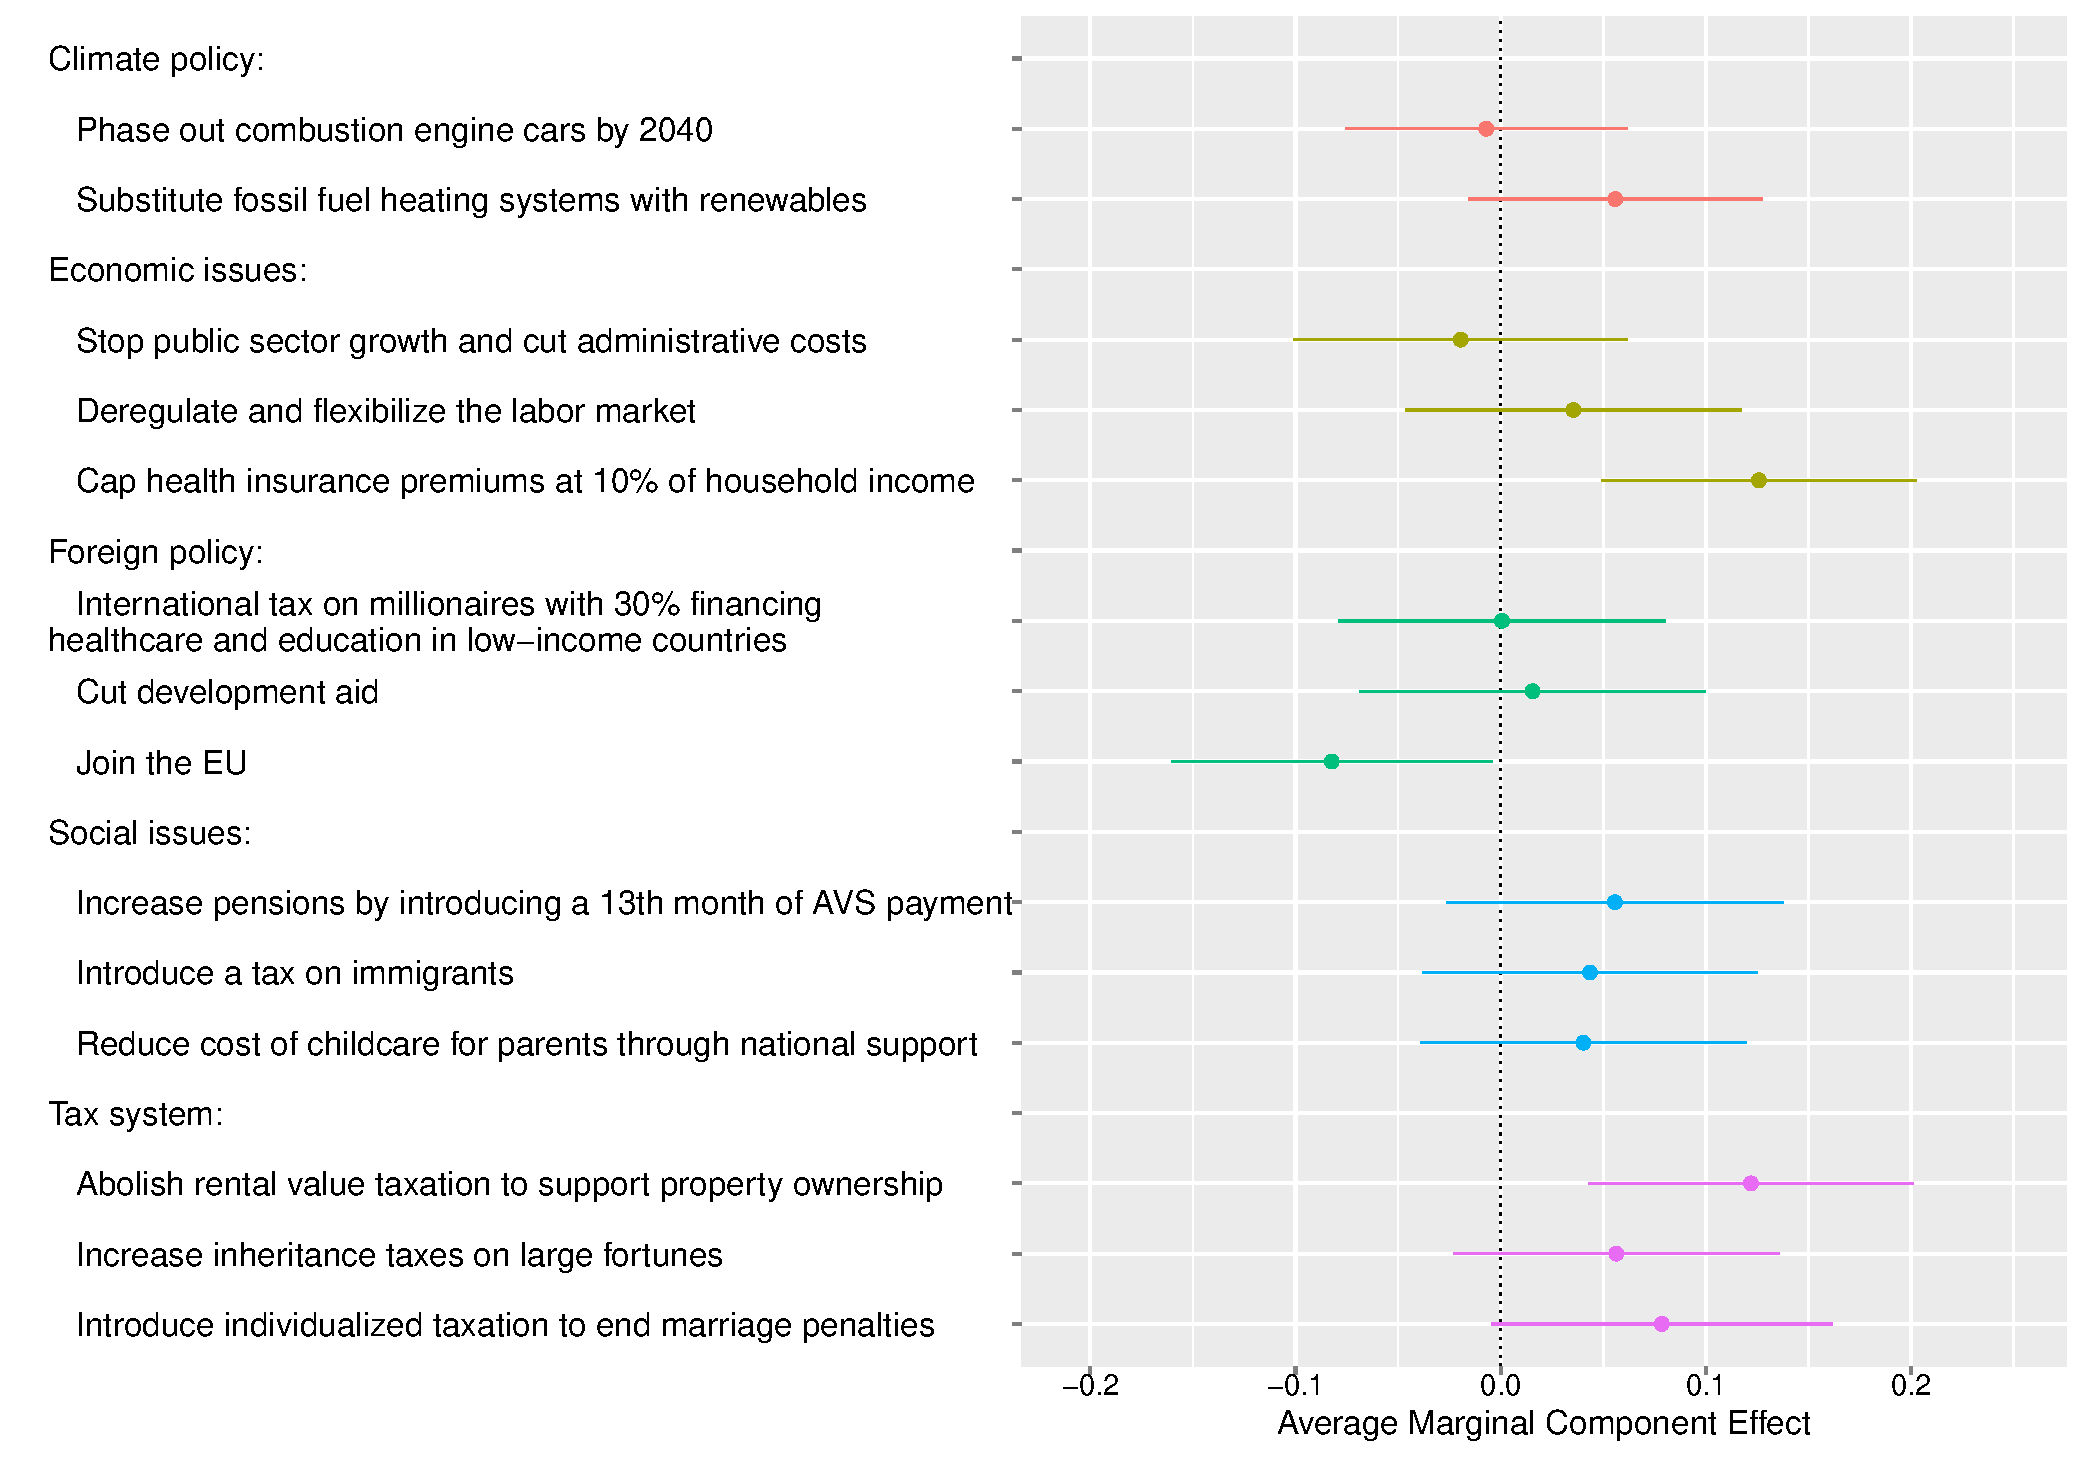
\includegraphics[width=\textwidth]{../figures/all/conjoint_EN-CH.pdf}} 
\end{figure} 

\begin{figure}[h!]
    \caption[Conjoint analysis in Japan]{Conjoint analysis in Japan (Average Marginal Component Effect). \hfill (Question~\ref{q:conjoint}).
    }\label{fig:conjoint_JP}
    \makebox[\textwidth][c]{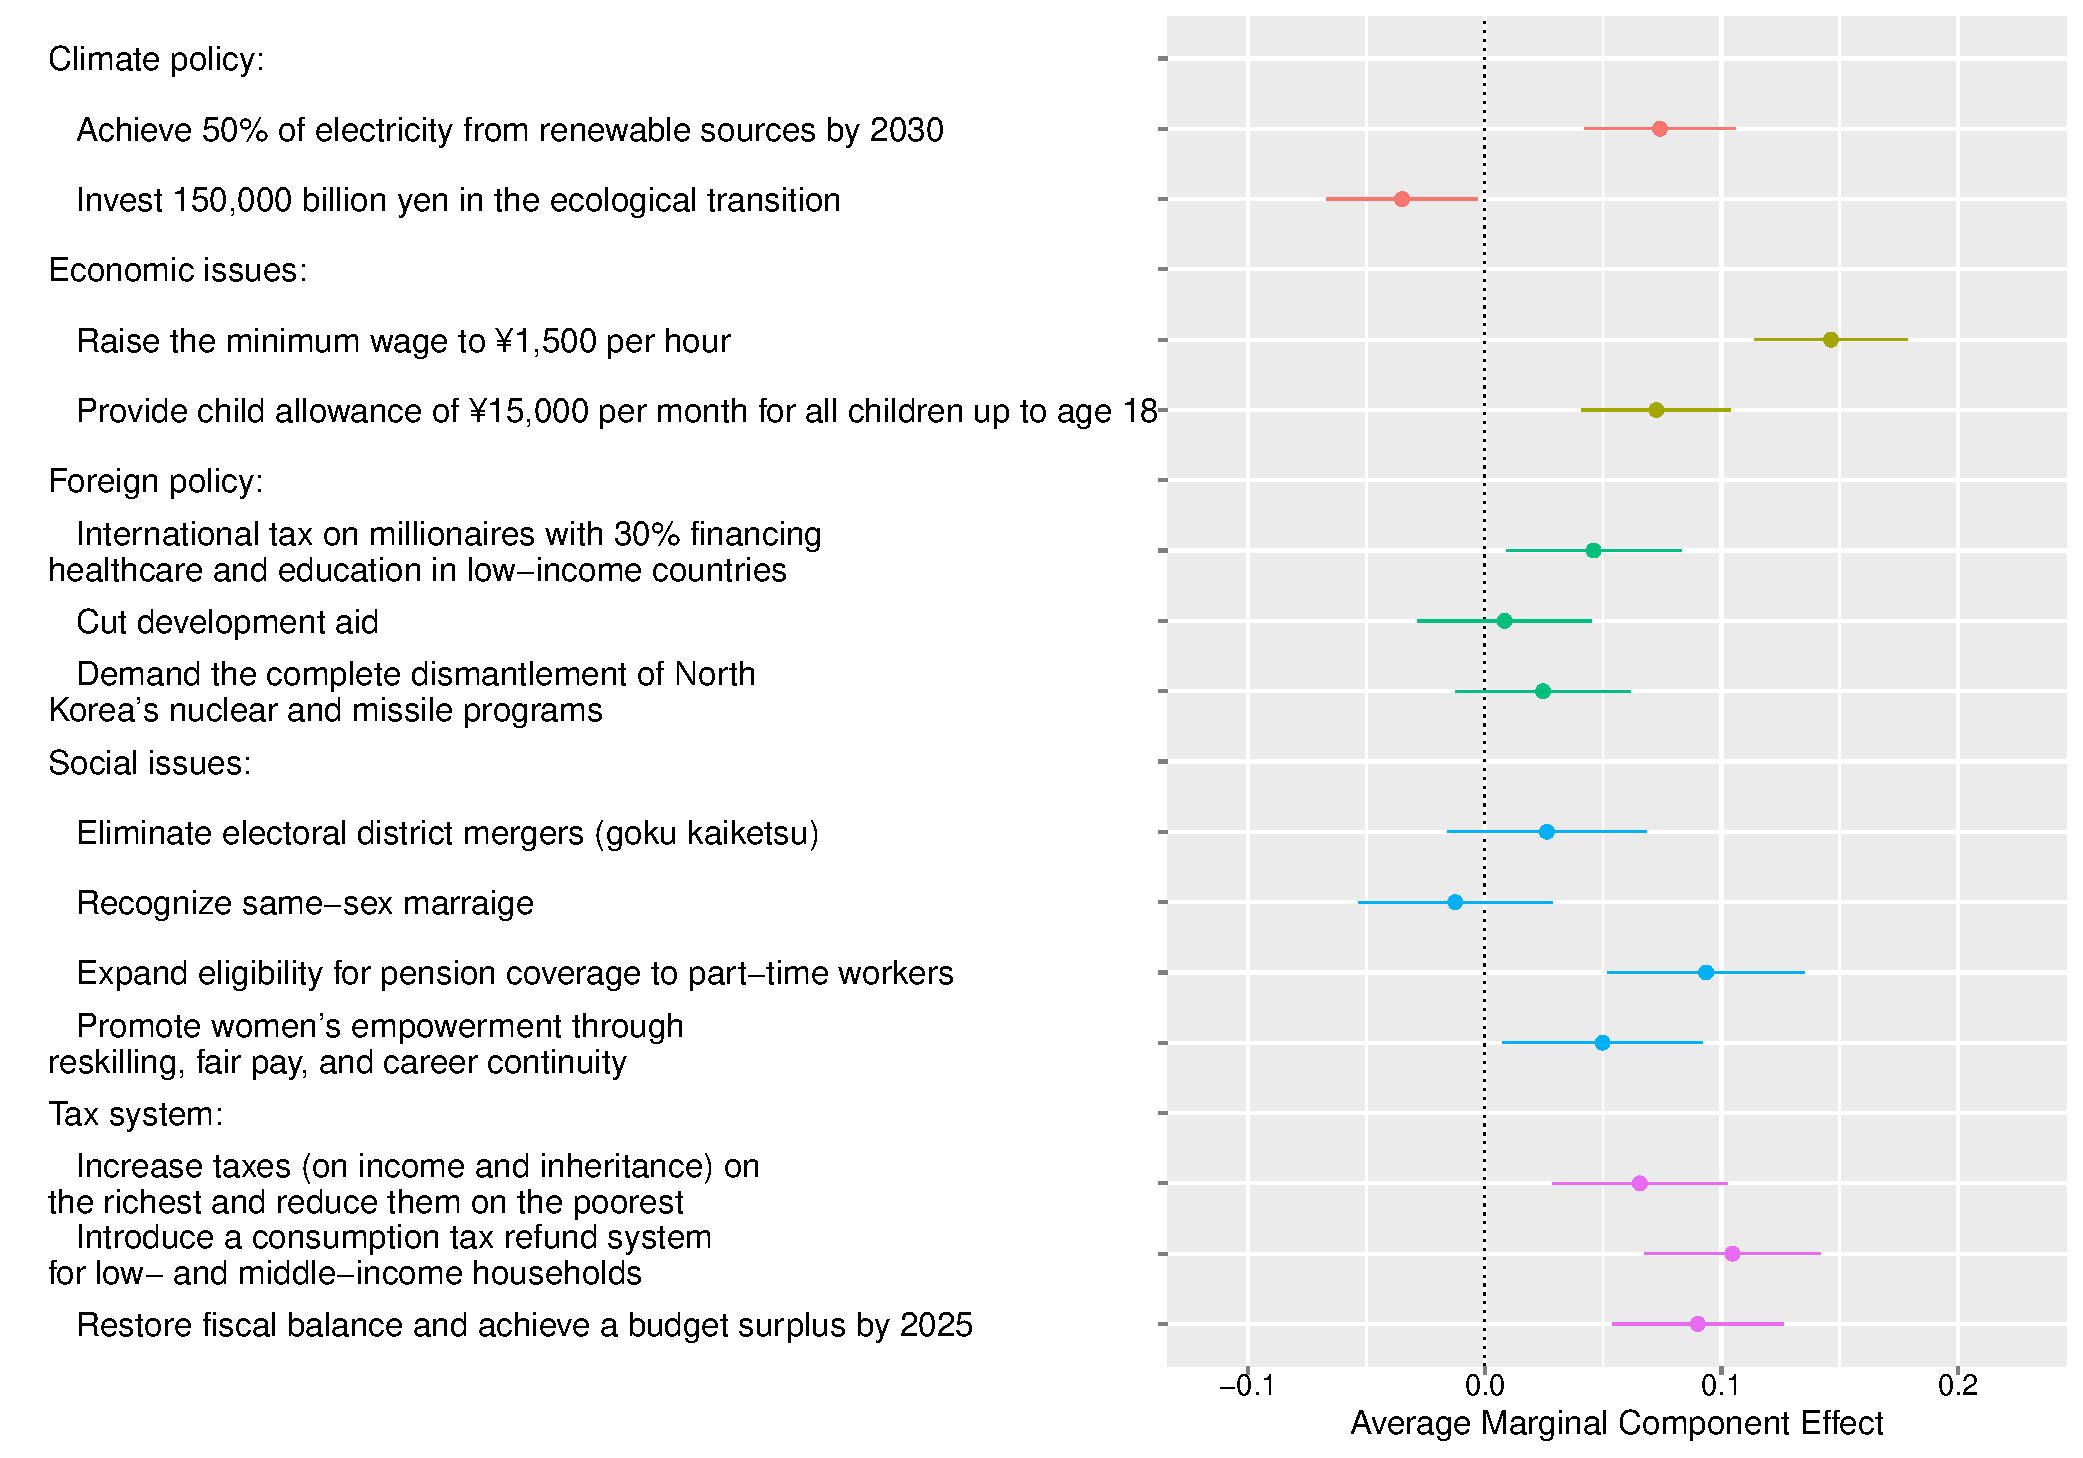
\includegraphics[width=\textwidth]{../figures/all/conjoint_EN-JA.pdf}} 
\end{figure} 
\begin{figure}[h!]
    \caption[Conjoint analysis in the U.S.]{Conjoint analysis in the U.S. (Average Marginal Component Effect). \hfill (Question~\ref{q:conjoint}).
    }\label{fig:conjoint_US}
    \makebox[\textwidth][c]{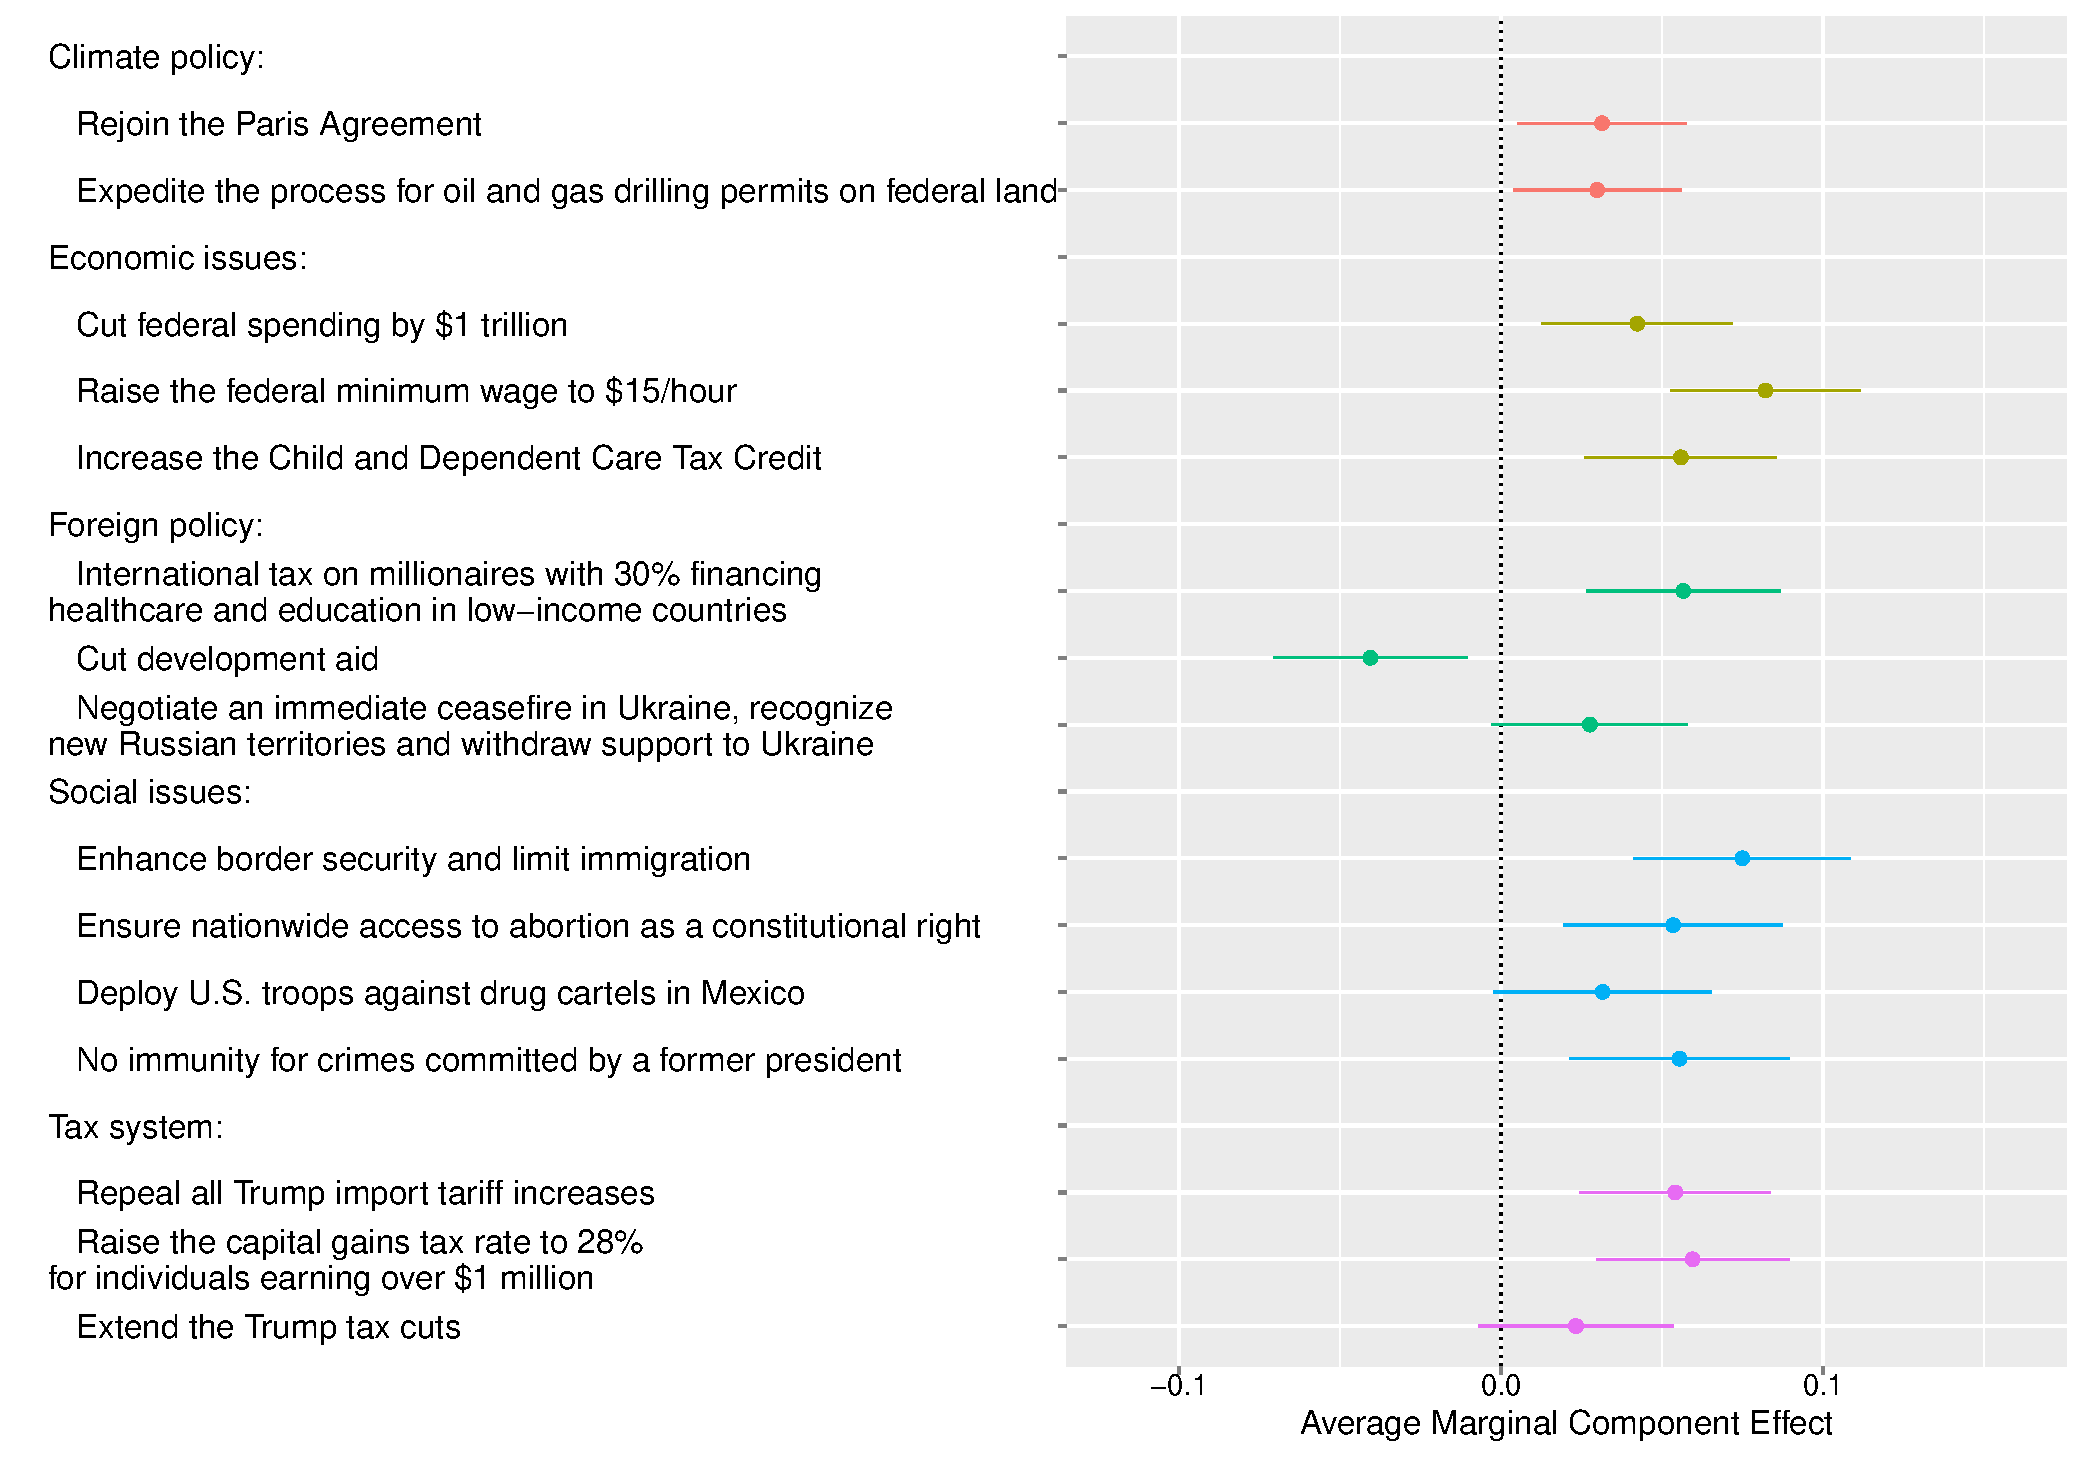
\includegraphics[width=\textwidth]{../figures/all/conjoint_EN.pdf}} 
\end{figure} 

\begin{figure}[h!]
    \caption[Conjoint analysis in France (French)]{Conjoint analysis in France (in French, cf. Figure \ref{fig:conjoint_FR} for English). \hfill (Question~\ref{q:conjoint}).
    }\label{fig:conjoint_FR_original}
    \makebox[\textwidth][c]{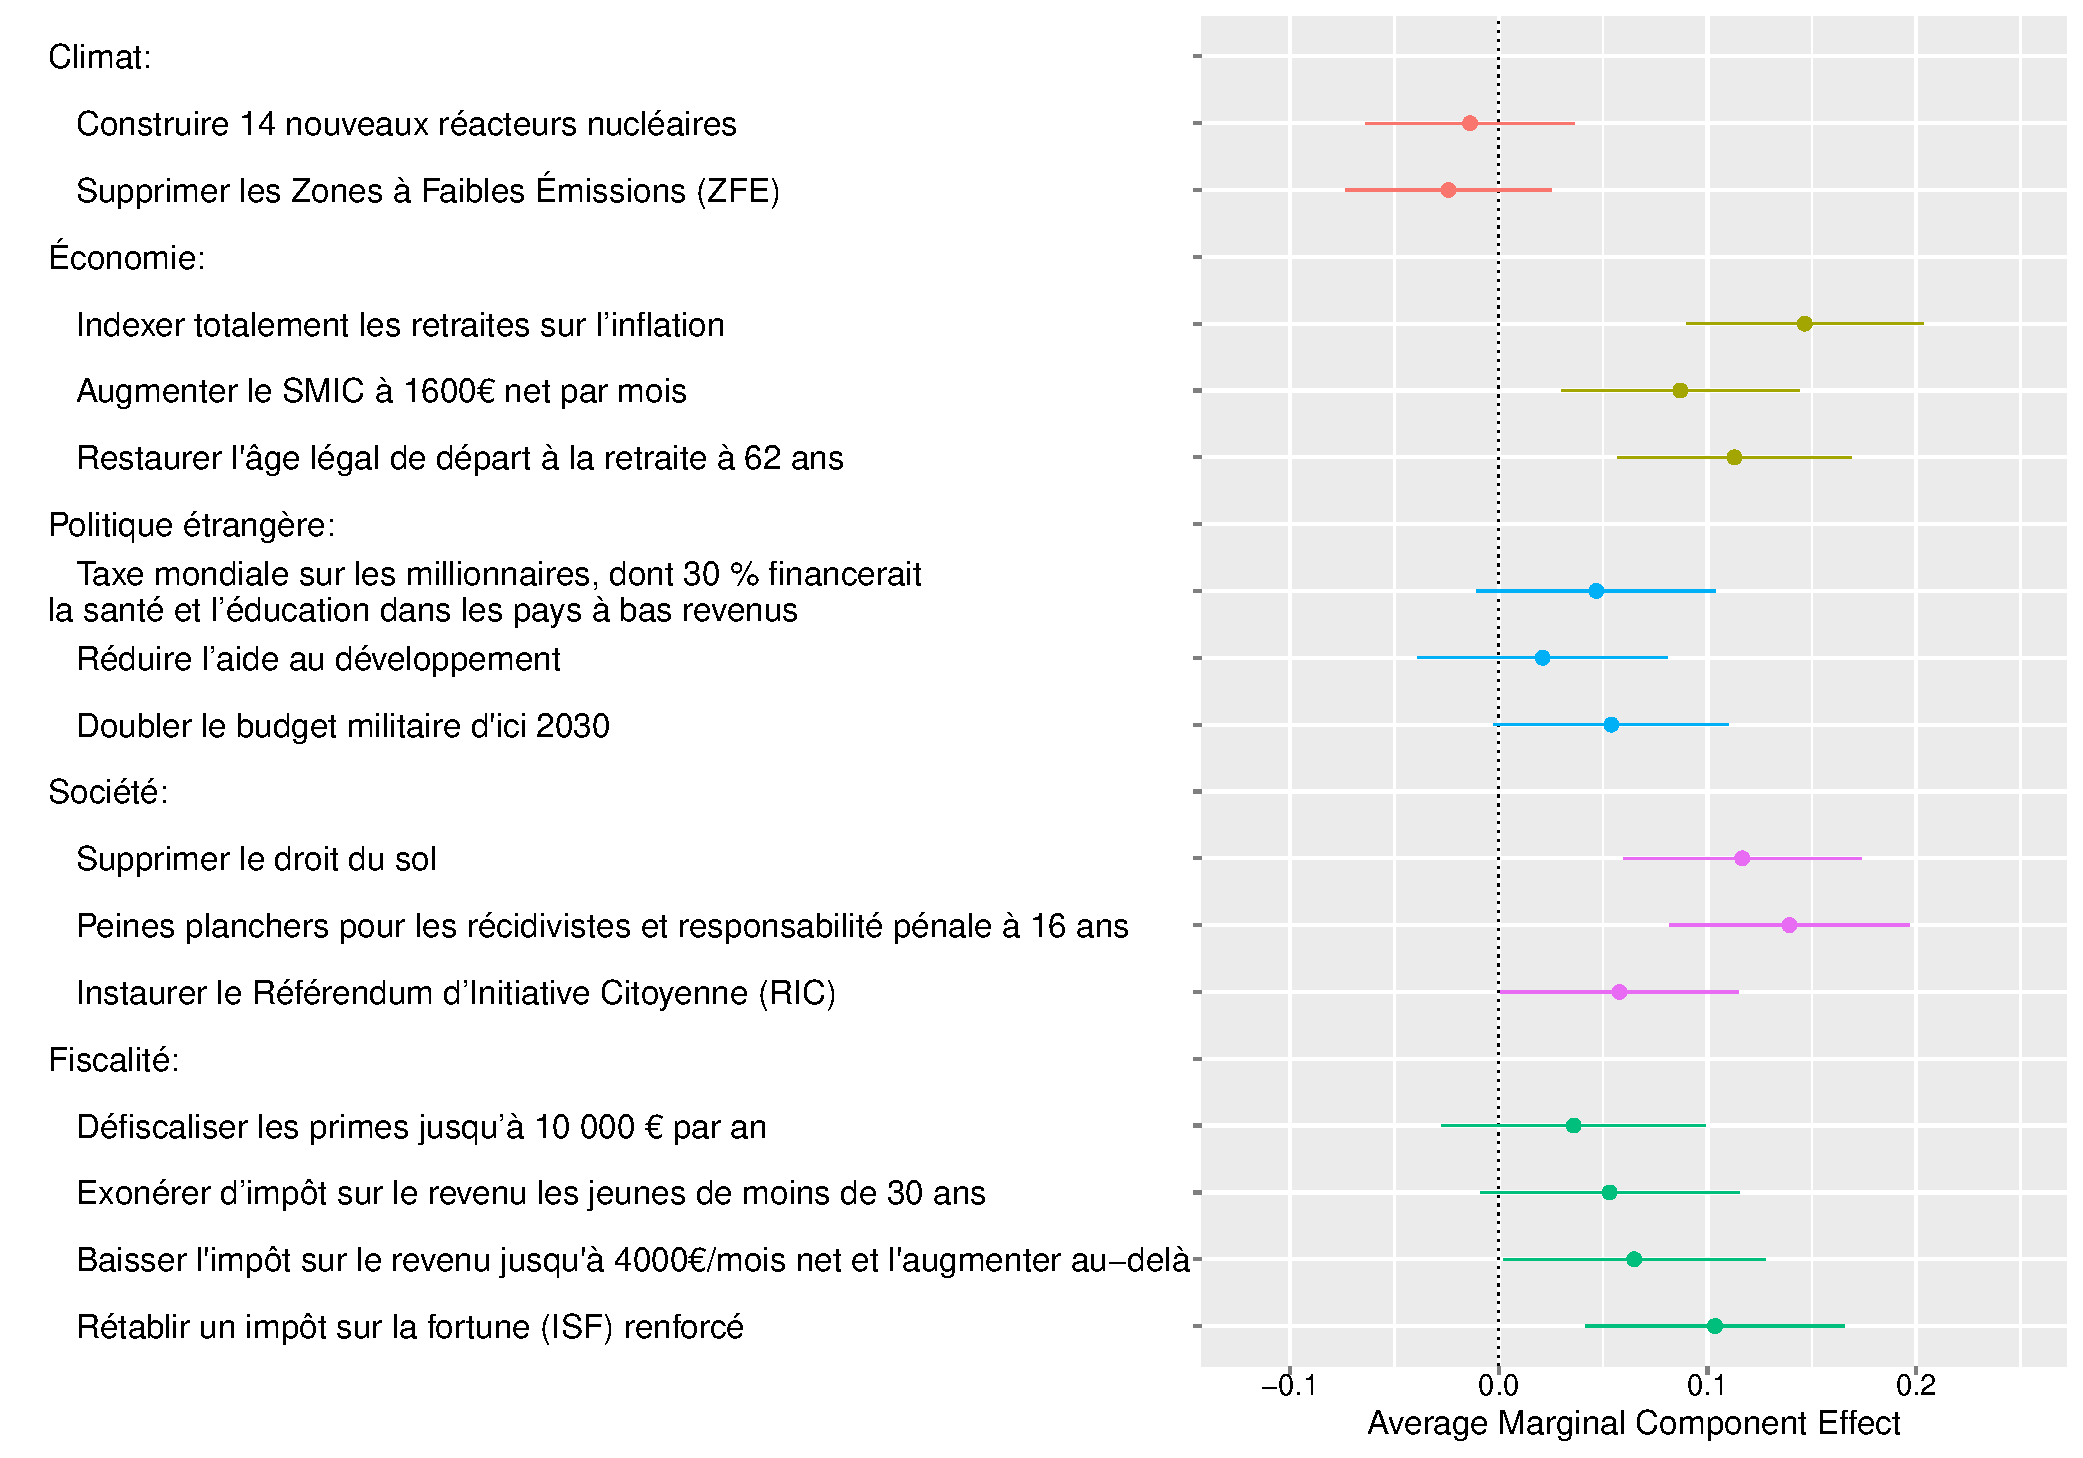
\includegraphics[width=\textwidth]{../figures/all/conjoint_FR.pdf}} 
\end{figure}

\begin{figure}[h!]
    \caption[Conjoint analysis in Germany (German)]{Conjoint analysis in Germany (in German, cf. Figure \ref{fig:conjoint_DE} for English). \hfill (Question~\ref{q:conjoint}).
    }\label{fig:conjoint_DE_original}
    \makebox[\textwidth][c]{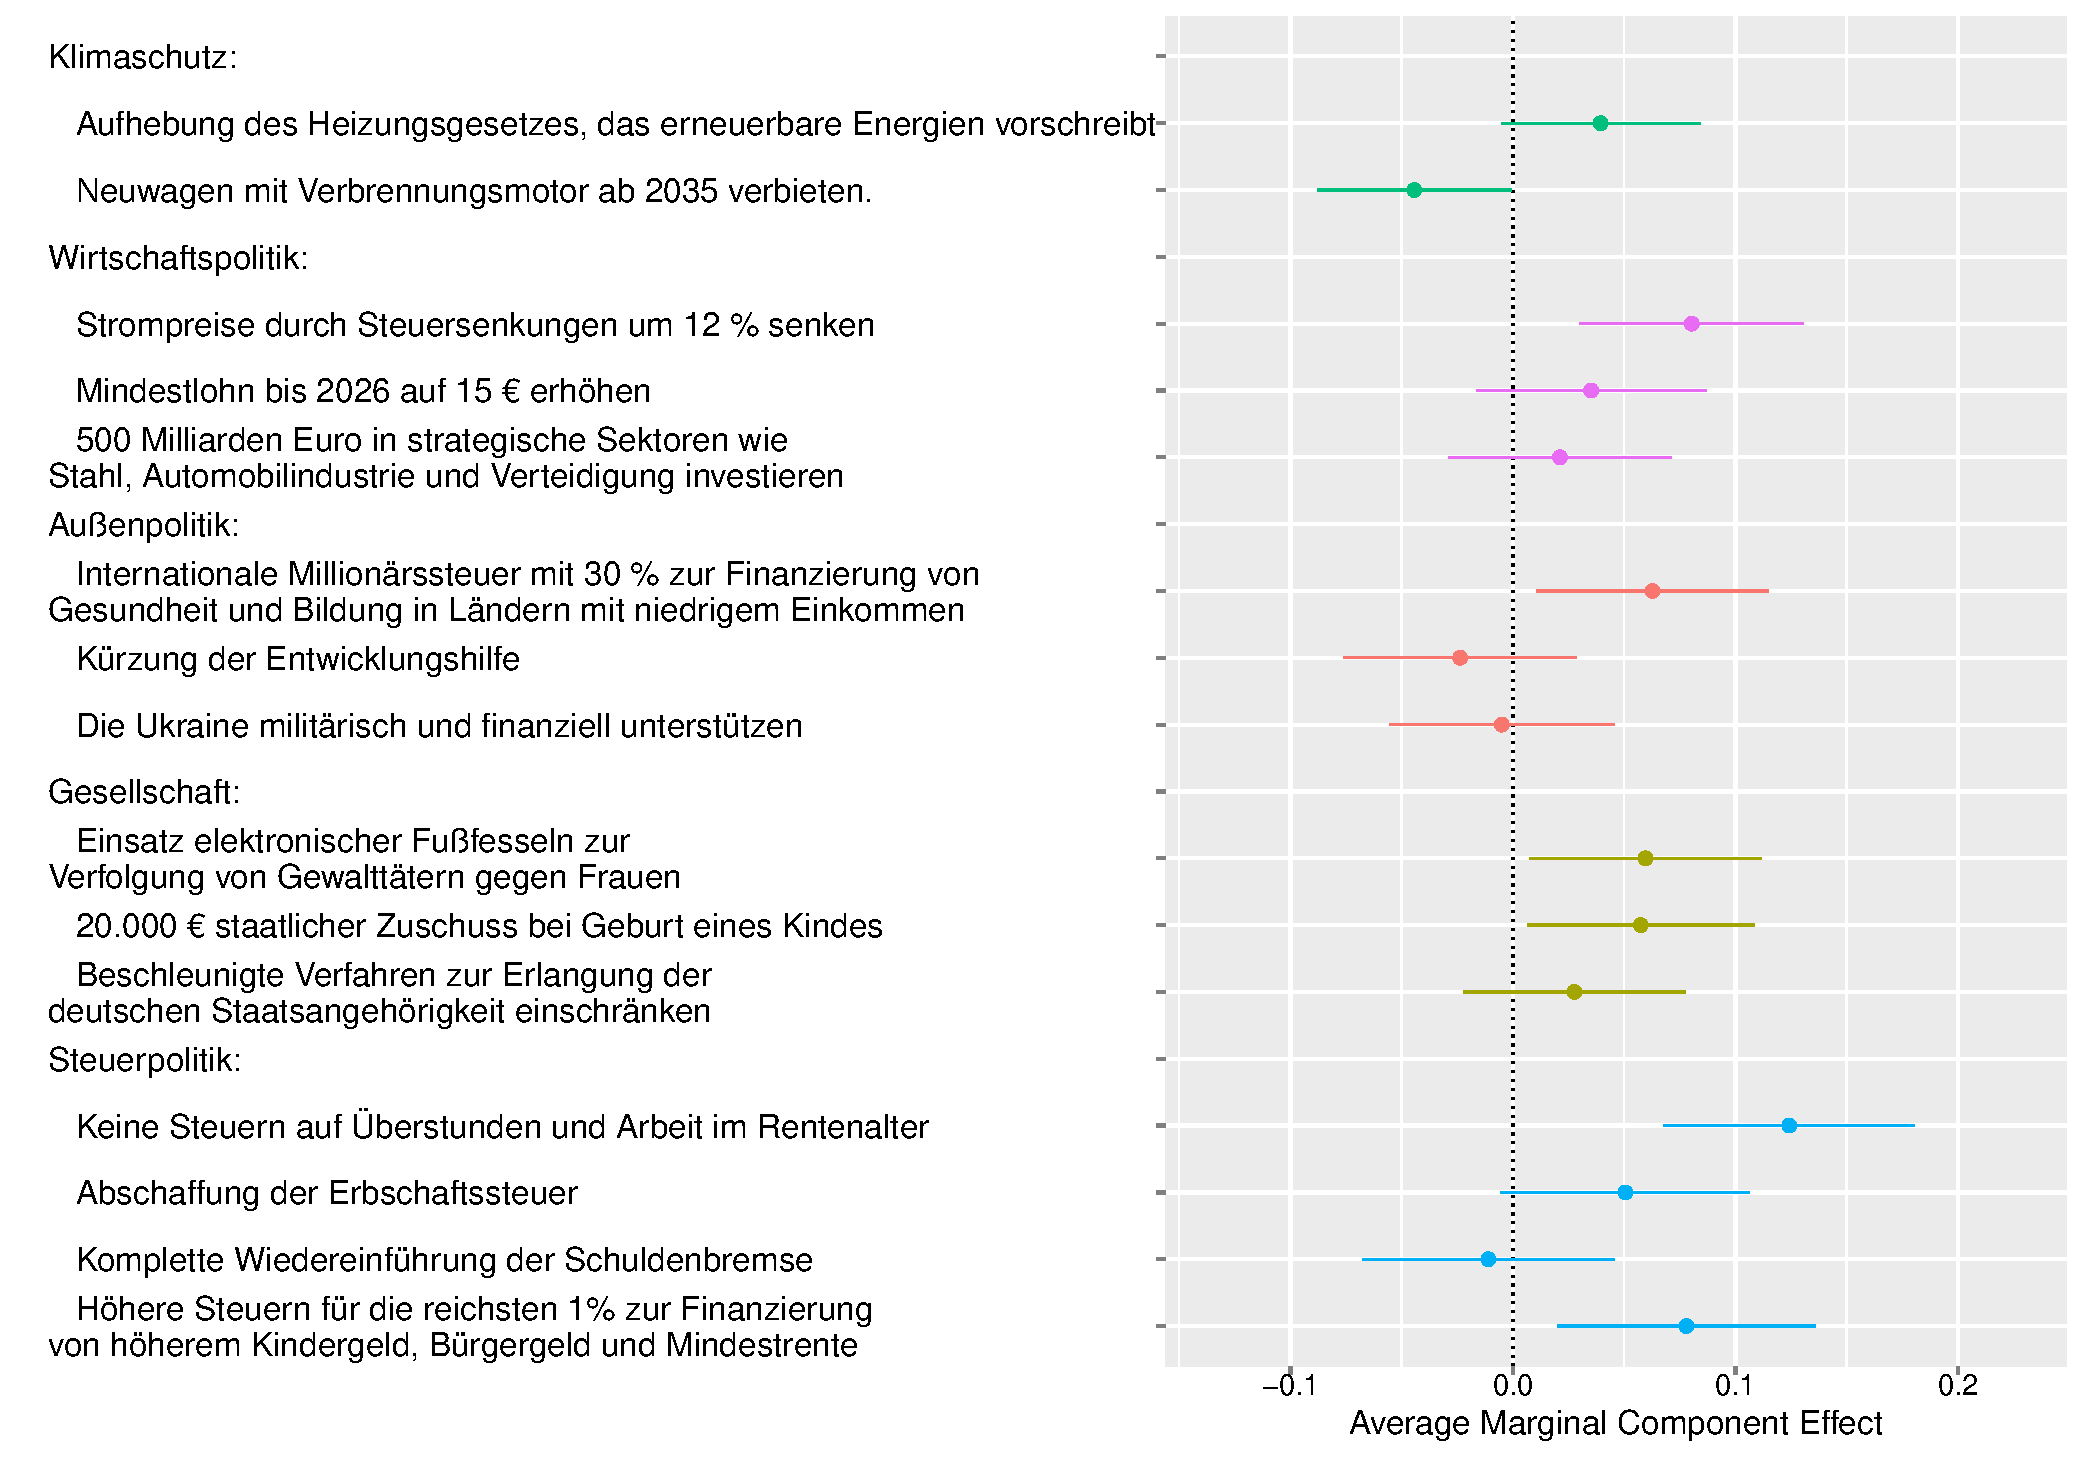
\includegraphics[width=\textwidth]{../figures/all/conjoint_DE.pdf}} 
\end{figure}

\begin{figure}[h!]
    \caption[Conjoint analysis in Italy (Italian)]{Conjoint analysis in Italy (in Italian, cf. Figure \ref{fig:conjoint_IT} for English). \hfill (Question~\ref{q:conjoint}).
    }\label{fig:conjoint_IT_original}
    \makebox[\textwidth][c]{\includegraphics[width=\textwidth]{../figures/all/conjoint_IT.pdf}} 
\end{figure}

\begin{figure}[h!]
    \caption[Conjoint analysis in Poland (Polish)]{Conjoint analysis in Poland (in Polish, cf. Figure \ref{fig:conjoint_PL} for English). \hfill (Question~\ref{q:conjoint}).
    }\label{fig:conjoint_PL_original}
    \makebox[\textwidth][c]{\includegraphics[width=\textwidth]{../figures/all/conjoint_PL.pdf}} 
\end{figure}

\begin{figure}[h!]
    \caption[Conjoint analysis in Spain (Spanish)]{Conjoint analysis in Spain (in Spanish, cf. Figure \ref{fig:conjoint_ES} for English). \hfill (Question~\ref{q:conjoint}).
    }\label{fig:conjoint_ES_original}
    \makebox[\textwidth][c]{\includegraphics[width=\textwidth]{../figures/all/conjoint_ES-ES.pdf}} 
\end{figure}

\begin{figure}[h!]
    \caption[Conjoint analysis in Japan (Japanese)]{Conjoint analysis in Japan (in Japanese, cf. Figure \ref{fig:conjoint_JP} for English). \hfill (Question~\ref{q:conjoint}).
    }\label{fig:conjoint_JP_original}
    \makebox[\textwidth][c]{\includegraphics[width=\textwidth]{../figures/JP/conjoint_JA.png}} 
\end{figure}

\begin{figure}[h!]
    \caption[Average preferred revenue split (\textit{few})]{Average preferred revenue split for a global wealth tax (variant \textit{few}). (Question~\ref{q:revenue_split_few}).
    }\label{fig:split_few_bars_nb0}
    \makebox[\textwidth][c]{\includegraphics[width=.8\textwidth]{../figures/country_comparison/split_few_bars_nb0.pdf}} 
\end{figure}

\begin{figure}[h!]
    \caption[Decomposition of preferred spending in revenue split]{Decomposition of preferred shares for each spending item in the revenue split (\textit{All} countries together; variant \textit{few}). (Question~\ref{q:revenue_split_few}).
    }\label{fig:split_few}
    \makebox[\textwidth][c]{\includegraphics[width=\textwidth]{../figures/all/split_few.pdf}} 
\end{figure}

\begin{figure}[h!]
    \caption[Decomposition of preferred spending in revenue split]{Decomposition of preferred shares for each spending item in the revenue split (\textit{All} countries together; variant \textit{many}). (Question~\ref{q:revenue_split_many}).
    }\label{fig:split_many}
    \makebox[\textwidth][c]{\includegraphics[width=.9\textwidth]{../figures/all/split_many.pdf}} 
\end{figure}

\begin{figure}[h!]
    \caption[Average preferred revenue split (\textit{many})]{Average preferred revenue split for a global wealth tax (variant \textit{many}). (Question~\ref{q:revenue_split_many}).
    }\label{fig:split_many_global_mean}
    \makebox[\textwidth][c]{\includegraphics[width=\textwidth]{../figures/country_comparison/split_many_global_mean.pdf}} 
\end{figure} 

% \begin{figure}[h!]
%     \caption[]{. (Question~\ref{q:gcs_support}).
%     }\label{fig:gcs_support}
%     \makebox[\textwidth][c]{\includegraphics[width=\textwidth]{../figures/country_comparison/split_few_mean.pdf}} 
% \end{figure}

\begin{figure}[h!]
    \caption[Amounts donated to plant trees.]{``By taking this survey, you will be automatically entered into a lottery to win up to [amount\_lottery: \$100]. \\Should you be selected in the lottery, you will have the option to channel a part of this additional compensation to the charity \textit{Just One Tree} to plant trees.\\\\\textbf{In case you win the lottery, what share of the [amount\_lottery: \$100 prize] would you donate to plant trees?}'' (Question~\ref{q:donation}).
    }\label{fig:donation}
    \makebox[\textwidth][c]{\includegraphics[width=.8\textwidth]{../figures/country_comparison/donation_agg_nolabel.pdf}} 
\end{figure}

% \begin{figure}[h!]
%     \caption[Support for the GCS and belief of support]{Support for the Global Climate Scheme and average belief regarding the support. (Questions~\ref{q:gcs_support}-\ref{q:gcs_belief_own}).
%     }\label{fig:gcs_belief}
%     \makebox[\textwidth][c]{\includegraphics[width=\textwidth]{../figures/country_comparison/gcs_belief_mean.pdf}} 
% \end{figure} 

\begin{figure}[h!]
    \caption[Support for the NCS, GCS, ICS, and belief of support for GCS]{Support for the National, Global, and International Climate Schemes, and median belief regarding the support for the GCS. (Questions~\ref{q:ncs_support}-\ref{q:ics_support}).
    }\label{fig:ncs_gcs_ics}
    \makebox[\textwidth][c]{\includegraphics[width=\textwidth]{../figures/country_comparison/ncs_gcs_ics_all_control_features_median_belief_various.pdf}} % ncs_gcs_ics_all_control_median_belief_various?
\end{figure} 
% TODO? CDF belief?

\begin{figure}[h!]
    \caption[Absolute support for plausible global redistribution policies]{Absolute support for plausible global redistribution policies (Percentage of \textit{Somewhat} or \textit{Strongly support}). See Figure~\ref{fig:solidarity_support_share} for the relative support. (Question~\ref{q:solidarity_support}).
    }\label{fig:solidarity_support_positive}
    \makebox[\textwidth][c]{\includegraphics[width=\textwidth]{../figures/country_comparison/solidarity_support_positive.pdf}} 
\end{figure}

\begin{figure}[h!]
    \caption[Average synthetic indicators of support for global redistribution]{Average synthetic indicators of support for global redistribution. (Question~\ref{q:solidarity_support}).
    }\label{fig:synthetic_indicators_mean}
    \makebox[\textwidth][c]{\includegraphics[width=\textwidth]{../figures/country_comparison/synthetic_indicators_mean.pdf}} 
\end{figure}


\begin{figure}[h!]
    \caption[Share of plausible global policies supported]{Share of plausible global redistribution policies supported (\textit{somewhat} or \textit{strongly}). (Question~\ref{q:solidarity_support}).
    }\label{fig:share_solidarity_supported}
    \makebox[\textwidth][c]{\includegraphics[width=\textwidth]{../figures/country_comparison/share_solidarity_supported_nolabel.pdf}} 
\end{figure}

\begin{figure}[h!]
    \caption[Share of plausible global policies opposed]{Share of plausible global redistribution policies opposed (\textit{somewhat} or \textit{strongly}). (Question~\ref{q:solidarity_support}).
    }\label{fig:share_solidarity_opposed}
    \makebox[\textwidth][c]{\includegraphics[width=\textwidth]{../figures/country_comparison/share_solidarity_opposed_nolabel.pdf}} 
\end{figure}

\begin{figure}[h!]
    \caption[Preferred NCQG, variant \textit{Short}]{Preferred North-to-South climate grant funding in 2035, specified in qualitative terms or in terms of who advocates for that amount (NCQG, variant \textit{Short}). (Question~\ref{q:ncqg}).
    }\label{fig:ncqg}
    \makebox[\textwidth][c]{\includegraphics[width=\textwidth]{../figures/country_comparison/ncqg_nolabel.pdf}} 
\end{figure}

\begin{figure}[h!]
    \caption[Preferred NCQG, variant \textit{Full}]{Preferred North-to-South climate grant funding in 2035, specified in money terms (NCQG, variant \textit{Full}). (Question~\ref{q:ncqg_full}).
    }\label{fig:ncqg_full}
    \makebox[\textwidth][c]{\includegraphics[width=\textwidth]{../figures/country_comparison/ncqg_full_nolabel.pdf}} 
\end{figure}

\begin{figure}[h!]
    \caption[Support for an international wealth depending on country coverage]{Support for an international wealth tax with 30\% of revenue funding LICs, depending on the country coverage (\textit{Yes}/\textit{No} question). (Questions~\ref{q:global_tax_support}-\ref{q:intl_tax_support}).
    }\label{fig:wealth_tax_heatmap}
    \makebox[\textwidth][c]{\includegraphics[width=\textwidth]{../figures/country_comparison/wealth_tax_support_positive.pdf}} 
\end{figure}

\begin{figure}[h!]
    \caption[Prefers a sustainable future]{Prefers a \textit{sustainable} rather than a \textit{business-as-usual} future. (Question~\ref{q:sustainable_future}).
    }\label{fig:sustainable_future}
    \makebox[\textwidth][c]{\includegraphics[width=.5\textwidth]{../figures/country_comparison/sustainable_future_nolabel.pdf}} 
\end{figure}

% \begin{figure}[h!]
%     \caption[Relative support for a global income tax on the richest to fund LICs]{Relative support for a global progressive income tax on the richest households to finance poverty reduction in the Global South (Percentage of \textit{Somewhat} or \textit{Strongly support} among non-\textit{Indifferent} responses). (Questions~\ref{q:top1_tax_support}-\ref{q:top3_tax_support}).
%     }\label{fig:top_tax_share}
%     \makebox[\textwidth][c]{\includegraphics[width=\textwidth]{../figures/country_comparison/top_tax_share.pdf}} 
% \end{figure}

\begin{figure}[h!]
    \caption[Relative support for a global income tax on the richest to fund LICs]{Relative support for a global progressive income tax on the richest households to finance global poverty reduction (Questions~\ref{q:top1_tax_support}-\ref{q:top3_tax_support}, Percentage of \textit{Somewhat} or \textit{Strongly support} among non-\textit{Indifferent} responses), and features of the tax presented to the respondents (Section~\ref{subsec:country_features}).
    }\label{fig:top_tax_share}
    \makebox[\textwidth][c]{\includegraphics[width=\textwidth]{../figures/country_comparison/top_tax_all_share_various.pdf}} % top_tax_share
\end{figure}

\begin{figure}[h!]
    \caption[Absolute support for an income tax on top 1\% to fund LICs]{Absolute support for a global progressive income tax on the richest households to finance global poverty reduction (Percentage of \textit{Somewhat} or \textit{Strongly support}). (Questions~\ref{q:top1_tax_support}-\ref{q:top3_tax_support}).
    }\label{fig:top_tax_positive}
    \makebox[\textwidth][c]{\includegraphics[width=\textwidth]{../figures/country_comparison/top_tax_positive.pdf}} 
\end{figure}

\begin{figure}[h!]
    \caption[Relative support for a global income tax among affected respondents]{Relative support for a global progressive income tax on the richest households to finance global poverty reduction \textit{among respondents affected by the tax} (Questions~\ref{q:top1_tax_support}-\ref{q:top3_tax_support}, Percentage of \textit{Somewhat} or \textit{Strongly support} among non-\textit{Indifferent} responses), and share of respondents affected by the tax (Section~\ref{subsec:country_features}).
    }\label{fig:top_tax_affected_share}
    \makebox[\textwidth][c]{\includegraphics[width=\textwidth]{../figures/country_comparison/top_tax_affected_share_various.pdf}} 
\end{figure}

% \begin{figure}[h!]
%     \caption[\textit{Right} or \textit{Best} way to transfer resources to LICs]{``How do you evaluate each of these channels to transfer resources to reduce poverty in LICs?''\\ Percentage of \textit{Right} or \textit{Best} way (other options: \textit{Wrong} or \textit{Acceptable} way). (Question~\ref{q:transfer_how}).
%     }\label{fig:transfer_how_positive}
%     \makebox[\textwidth][c]{\includegraphics[width=\textwidth]{../figures/country_comparison/transfer_how_positive.pdf}} 
% \end{figure}

\begin{figure}[h!]
    \caption[\textit{Best} way to transfer resources to LICs]{``How do you evaluate each of these channels to transfer resources to reduce poverty in LICs?''\\ Percentage of \textit{Best} way (other options: \textit{Right}, \textit{Wrong} or \textit{Acceptable} way). (Question~\ref{q:transfer_how}).
    }\label{fig:transfer_how_above_one}
    \makebox[\textwidth][c]{\includegraphics[width=\textwidth]{../figures/country_comparison/transfer_how_above_one.pdf}} 
\end{figure}

\begin{figure}[h!]
    \caption[\textit{Wrong} way to transfer resources to LICs]{``How do you evaluate each of these channels to transfer resources to reduce poverty in LICs?''\\ Percentage of \textit{Wrong} way (other options: \textit{Best}, \textit{Right} or \textit{Acceptable} way). (Question~\ref{q:transfer_how}).
    }\label{fig:transfer_how_negative}
    \makebox[\textwidth][c]{\includegraphics[width=\textwidth]{../figures/country_comparison/transfer_how_negative.pdf}} 
\end{figure}

\begin{figure}[h!]
    \caption[Support for making all countries' GDP p.c. converge by 2100]{``Should governments actively cooperate to have all countries converge in terms of GDP per capita by the end of the century?'' (Question~\ref{q:convergence_support}).
    }\label{fig:convergence_support}
    \makebox[\textwidth][c]{\includegraphics[width=.7\textwidth]{../figures/country_comparison/convergence_support_nolabel.pdf}} 
\end{figure}

\begin{figure}[h!]
    \caption[Willingness to participate in a global movement for sustainable development]{``If there was a worldwide movement in favor of a global program to tackle climate change, implement taxes on millionaires and fund poverty reduction in low-income countries, to what extent would you be willing to be part of that movement? (Multiple answers possible)'' (Question~\ref{q:global_movement}).
    }\label{fig:global_movement}
    \makebox[\textwidth][c]{\includegraphics[width=\textwidth]{../figures/country_comparison/global_movement_positive.pdf}} 
\end{figure}

\begin{figure}[h!]
    \caption[Would vote for a party in a global coalition for sustainable development]{``Let us call "your political party" the party you voted for in the last election, or the party that represents your views most closely.~\\\textbf{Imagine }there was \textbf{a worldwide coalition} of political parties in favor of a common program \textbf{to tackle climate change, implement taxes on millionaires and fund poverty reduction in low-income countries}.~\\\\\textbf{Would you be more likely to vote for your party if it were part of that coalition?}'' (Question~\ref{q:vote_intl_coalition}).
    }\label{fig:vote_intl_coalition}
    \makebox[\textwidth][c]{\includegraphics[width=.7\textwidth]{../figures/country_comparison/vote_intl_coalition_nolabel.pdf}} 
\end{figure}

\begin{figure}[h!]
    \caption[Agreement with rationales for global redistribution]{``Some people think that high-income countries should support low-income countries.~\\Among the different reasons given, which ones do you agree with? (Multiple answers possible)'' (Question~\ref{q:why_hic_help_lic}).
    }\label{fig:why_hic_help_lic}
    \makebox[\textwidth][c]{\includegraphics[width=\textwidth]{../figures/country_comparison/why_hic_help_lic_positive.pdf}} 
\end{figure}

\begin{figure}[h!]
    \caption[Support for reparations for colonization and slavery]{``Some people argue that Western countries owe reparations for colonization and slavery to former colonies and descendants of slaves. \\Reparations could take the form of funding education and facilitating technology transfers, to address unequal opportunities passed down from the past. \\\\\textbf{Do you support or oppose reparations} of this kind \textbf{for colonization and slavery?~}'' (Question~\ref{q:reparations_support}).
    }\label{fig:reparations_support}
    \makebox[\textwidth][c]{\includegraphics[width=.9\textwidth]{../figures/country_comparison/reparations_support_nolabel.pdf}} 
\end{figure}

\begin{figure}[h!]
    \caption[Median custom redistribution]{Global redistribution obtained from median custom parameters: 49\% of winners; 18\% of losers; degree of redistribution of 5 (out of 10). (Question~\ref{q:custom_redistr}).
    }\label{fig:custom_redistr_median}
    \makebox[\textwidth][c]{\includegraphics[width=.9\textwidth]{../figures/questionnaire/survey_custom_redistr_median_zoom.png}} 
\end{figure} 

\begin{figure}[h!]
    \caption[Average custom redistribution]{Average custom global redistribution. (Question~\ref{q:custom_redistr}).
    }\label{fig:custom_redistr_mean}
    \makebox[\textwidth][c]{\includegraphics[width=.9\textwidth]{../figures/mean_custom_redistr/all_satisfied.png}} 
\end{figure}

\begin{figure}[h!]
    \caption[Average answers to custom redistribution]{Mean answers to custom redistribution. (Question~\ref{q:custom_redistr}).
    }\label{fig:custom_redistr_most}
    \makebox[\textwidth][c]{\includegraphics[width=\textwidth]{../figures/country_comparison/custom_redistr_most_mean.pdf}} 
\end{figure} 

\begin{figure}[h!]
    \caption[Average answers to custom redistribution among satisfied]{Mean answers to custom redistribution among respondents satisfied with their custom redistribution. (Question~\ref{q:custom_redistr}).
    }\label{fig:custom_redistr_satisfied_mean}
    \makebox[\textwidth][c]{\includegraphics[width=\textwidth]{../figures/country_comparison/custom_redistr_satisfied_mean.pdf}} 
\end{figure} 

\begin{figure}[h!]
    \caption[Median answers to custom redistribution among satisfied]{Median answers to custom redistribution among respondents satisfied with their custom redistribution. (Question~\ref{q:custom_redistr}).
    }\label{fig:custom_redistr_satisfied_median}
    \makebox[\textwidth][c]{\includegraphics[width=\textwidth]{../figures/country_comparison/custom_redistr_satisfied_median.pdf}} 
\end{figure} 

\begin{figure}[h!]
    \caption[Preferred share of winners in the custom redistributions]{Preferred share of winners in the custom redistributions among satisfied respondents. (Question~\ref{q:custom_redistr}).
    }\label{fig:custom_redistr_winners_agg}
    \makebox[\textwidth][c]{\includegraphics[width=\textwidth]{../figures/all/custom_redistr_winners_agg.pdf}} 
\end{figure} 

\begin{figure}[h!]
    \caption[Preferred share of losers in the custom redistributions]{Preferred share of losers in the custom redistributions among satisfied respondents. (Question~\ref{q:custom_redistr}).
    }\label{fig:custom_redistr_losers_agg}
    \makebox[\textwidth][c]{\includegraphics[width=\textwidth]{../figures/all/custom_redistr_losers_agg.pdf}} 
\end{figure} 

\begin{figure}[h!]
    \caption[Minimum income implied by custom redistributions]{Minimum worldwide income implied by custom redistributions among satisfied respondents (in PPP \$ per month). (Question~\ref{q:custom_redistr}).
    }\label{fig:custom_redistr_income_min_ceiling}
    \makebox[\textwidth][c]{\includegraphics[width=\textwidth]{../figures/all/custom_redistr_income_min_ceiling.pdf}} 
\end{figure} 

\begin{figure}[h!]
    \caption[Transfer implied by custom redistributions]{Rich-to-poor transfer implied by custom redistributions among satisfied respondents. (Question~\ref{q:custom_redistr}).
    }\label{fig:custom_redistr_transfer_ceiling}
    \makebox[\textwidth][c]{\includegraphics[width=\textwidth]{../figures/all/custom_redistr_transfer_ceiling.pdf}} 
\end{figure} 

% \begin{figure}[h!]
%     \caption[Average well-being depending on the variant]{Average subjective well-being, depending on the variant. (Question~\ref{q:well_being}).
%     }\label{fig:well_being}
%     \makebox[\textwidth][c]{\includegraphics[width=\textwidth]{../figures/country_comparison/well_being_mean.pdf}} 
% \end{figure}

\begin{figure}[h!]
    \caption[Comprehension question on GCS]{``\textit{Comprehension question: one respondent with the expected answer will get [amount\_lottery: \$100].}\\\\How would gasoline prices change as a result of the Global Climate Scheme? \\Gasoline prices would...'' (Correct answer: \textit{increase}) (Question~\ref{q:gcs_comprehension}).
    }\label{fig:gcs_comprehension}
    \makebox[\textwidth][c]{\includegraphics[width=.5\textwidth]{../figures/country_comparison/gcs_comprehension_nolabel.pdf}} 
\end{figure}

\begin{figure}[h!]
    \caption[Relative agreement: ``My taxes should go towards solving global problems'']{Relative agreement for: ``To what extent do you agree or disagree with the following statement? "My taxes should go towards solving global problems."'' (Percentage of \textit{Agree} or \textit{Strongly agree} among non-\textit{Neither agree nor disagree} responses). (Question~\ref{q:my_tax_global_nation}).
    }\label{fig:my_tax_global_nation_share}
    \makebox[\textwidth][c]{\includegraphics[width=\textwidth]{../figures/country_comparison/my_tax_global_nation_share.pdf}} 
\end{figure}

\begin{figure}[h!]
    \caption[Absolute agreement: ``My taxes should go towards solving global problems'']{Absolute agreement for: ``To what extent do you agree or disagree with the following statement? "My taxes should go towards solving global problems."'' (Percentage of \textit{Agree} or \textit{Strongly agree}). (Question~\ref{q:my_tax_global_nation}).
    }\label{fig:my_tax_global_nation_positive}
    \makebox[\textwidth][c]{\includegraphics[width=\textwidth]{../figures/country_comparison/my_tax_global_nation_positive.pdf}} 
\end{figure}

\begin{figure}[h!]
    \caption[Moral circle]{``Which group of people do you advocate for when you vote?''\footref{fn:group_defended} (Question~\ref{q:group_defended}).
    }\label{fig:group_defended_all}
    \makebox[\textwidth][c]{\includegraphics[width=.9\textwidth]{../figures/country_comparison/group_defended_nolabel.pdf}} 
\end{figure}

% \begin{figure}[h!]
%     \caption[Moral circle (heatmap)]{``Which group of people do you advocate for when you vote?'' (Question~\ref{q:group_defended}).
%     }\label{fig:group_defended_heatmap}
%     \makebox[\textwidth][c]{\includegraphics[width=.9\textwidth]{../figures/country_comparison/group_defended_5_positive.pdf}} 
% \end{figure}

\begin{figure}[h!]
    \caption[Feeling that the survey was politically biased]{``Do you feel that this survey was politically biased?'' (Question~\ref{q:survey_biased}).
    }\label{fig:survey_biased}
    \makebox[\textwidth][c]{\includegraphics[width=.5\textwidth]{../figures/country_comparison/survey_biased_nolabel.pdf}} 
\end{figure}

\begin{figure}[h!]
    \caption[Manual classification of \textit{feedback} fields]{Manual classification of \textit{feedback} fields: ``The survey is nearing completion. You can now enter any comments, thoughts, or suggestions in the field below.'' (Question~\ref{q:comment_field}).
    }\label{fig:comment_field}
    \makebox[\textwidth][c]{\includegraphics[width=.9\textwidth]{../figures/country_comparison/comment_manual_positive.pdf}} 
\end{figure}

% \begin{figure}[h!]
%     \caption[]{. (Questions~\ref{q:gcs_support}).
%     }\label{fig:radical_redistr_positive}
%     \makebox[\textwidth][c]{\includegraphics[width=.9\textwidth]{../figures/country_comparison/radical_redistr_positive.pdf}} 
% \end{figure} % TODO?

% Pb of translation in Saudi Arabia: millionaire has probably be understood in SAR (= $250k)
\begin{figure}[h!]
    \caption[Likelihood of becoming a millionaire]{``How likely are you to become a millionaire at some point in your life?'' (Question~\ref{q:millionaire}).
    }\label{fig:millionaire}
    \makebox[\textwidth][c]{\includegraphics[width=.8\textwidth]{../figures/country_comparison/millionaire_nolabel.pdf}} 
\end{figure}

\begin{figure}[h!]
    \caption[Foreign origin]{``Were you or your parents born in a foreign country?'' (Question~\ref{q:foreign}).
    }\label{fig:foreign}
    \makebox[\textwidth][c]{\includegraphics[width=.7\textwidth]{../figures/country_comparison/foreign_born_family_nolabel.pdf}} 
\end{figure}

\begin{figure}[h!]
    \caption[Vote in the last election compared to actual results (among voters)]{Vote in the last election, compared to actual results among voters. (Questions~\ref{q:voted}, \ref{q:vote}).
    }\label{fig:vote_pnr_out}
    \makebox[\textwidth][c]{\includegraphics[width=\textwidth]{../figures/country_comparison/vote_pnr_out.pdf}} 
\end{figure}

\begin{figure}[h!]
    \caption[Vote in the last election compared to actual results (entire population)]{Vote in the last election, compared to actual results on the entire population. (Questions~\ref{q:voted}, \ref{q:vote}).
    }\label{fig:vote_representativeness}
    \makebox[\textwidth][c]{\includegraphics[width=.9\textwidth]{../figures/country_comparison/vote_representativeness.pdf}} 
\end{figure}

% \begin{figure}[h!]
%     \caption[]{. (Question~\ref{q:gcs_support}).
%     }\label{fig:gcs_support}
%     \makebox[\textwidth][c]{\includegraphics[width=.9\textwidth]{../figures/country_comparison/gcs_support.pdf}} 
% \end{figure}


\renewcommand{\theenumi}{\arabic{enumi}}
\clearpage
\section{Questionnaire}\label{app:questionnaire}
The U.S. version of the questionnaire is presented. Features that vary across countries are put in square brackets within the question tex, as follows: [feature\_name: U.S. value]. Features values for each country are given in \href{https://github.com/bixiou/robustness_global_redistr/raw/main/questionnaire/sources.xlsx}{this spreadsheet}. 
Random branches or conditions for displaying the question are specified in square brackets before the question text (cf. Figure \ref{fig:flow} for the survey flow). The question text is followed by square brackets that refer to Figures and Tables presenting the question results, and the variable name(s) corresponding to the question. Finally, response options are displayed in italics. 
Unless otherwise specified, response is compulsory and a single response much be chosen.

\subsection*{Welcome} 
 \begin{enumerate} 
\item  \label{q:consent} Welcome to this survey!\\
This survey is \textbf{anonymous }and is conducted \textbf{for research} purposes on a representative sample of [sample\_size: 3,000] [nationality: American people].\\
~\\
It takes around 20 min to complete.\\
~\\
The survey contains lotteries and awards for those who get the correct answer to some comprehension questions.\\
If you are attentive and lucky, \textbf{you can win up to [amount\_lottery: \$100]}.\\
~\\
Please answer every question carefully.\\
~\\
By clicking on the button below, you consent to the terms and conditions.

\end{enumerate} 

 \subsection*{Socio-demographics} 
 \begin{enumerate}[resume] 
\item  \label{q:gender} What is your gender? [%\textit{Figure \ref{fig:gender}}; 
\verb|gender|]
  \\ \textit{Woman; Man; Other}

\item  \label{q:hidden_country} What is your country? [%\textit{Figure \ref{fig:hidden_country}}; 
\verb|hidden_country|]


\item  \label{q:age_exact} What is your age? [%\textit{Figure \ref{fig:age_exact}}; 
\verb|age_exact, age|]
  \\ \textit{Below 18; 18 to 20; 21 to 24; 25 to 29; 30 to 34; 35 to 39; 40 to 44; 45 to 49; 50 to 54; 55 to 59; 60 to 64; 65 to 69; 70 to 74; 75 to 79; 80 to 84; 85 to 89; 90 to 99; 100 or above}

\item  \label{q:foreign} Were you or your parents born in a foreign country?~ [%\textit{Figure \ref{fig:foreign}}; % TODO
\verb|foreign|]
  \\ \textit{Yes, I was born in a foreign country; Not me but both my parents were born in a foreign country; Not me but one of my parents was born in a foreign country; No, I was born in this country and my parents too}

\item  \label{q:couple} Do you live with your partner (if you have one)? [%\textit{Figure \ref{fig:couple}}; 
\verb|couple|]
  \\ \textit{Yes; No}

\item  \label{q:hh_size} How many people are there in your household? \\The household includes: \textbf{you}, your spouse, \textbf{your family members} who live with you, and your dependents (not flatmates). [%\textit{Figure \ref{fig:hh_size}}; 
\verb|hh_size|]
  \\ \textit{1; 2; 3; 4; 5 or more}

\item  \label{q:Nb_children__14} How many children under the age of 14 live with you? [%\textit{Figure \ref{fig:Nb_children__14}}; 
\verb|Nb_children__14|]
  \\ \textit{0; 1; 2; 3; 4 or more}

\item ~[new page] \label{q:race} [\textit{Only in: US}] What race or ethnicity do you identify with? (Multiple answers are possible) [%\textit{Figure \ref{fig:race}}; 
\verb|race|]
  \\ \textit{White; Black or African American; Hispanic; Asian; American Indian or Alaskan Native; Native Hawaiian or Pacific Islander; Other; Prefer not to say}

\item  \label{q:income} What is the \textbf{[periodicity\_text: monthly] [income\_type: gross] income of your household}, [income\_type\_long: after taxes and transfers]?

This includes all sources of income: wages, pensions, welfare payments, property income, dividends, self-employment earnings, Social Security benefits, and income from other sources. [%\textit{Figure \ref{fig:income}}; 
\verb|income|]
  \\ ~[\textit{All but RU, US}: Custom thresholds, taking into account household composition Questions \ref{q:couple}-\ref{q:Nb_children__14}, and corresponding to the country's deciles and quartiles of standard of living, cf. the sheet ``Income'' in \href{https://github.com/bixiou/robustness_global_redistr/raw/main/questionnaire/source.xlsx}{this spreadsheet}; \\ \textit{RU, US}: Items based on household total income deciles and quartiles, namely in US: \textit{Less than \$17,000; between \$17,001 and \$30,000; between \$30,001 and \$36,000; between \$36,001 and \$43,000; between \$43,001 and \$56,000; between \$56,001 and \$72,000; between \$72,001 and \$91,000; between \$91,001 and \$115,000; between \$115,001 and \$130,000; between \$130,001 and \$150,000; between \$150,001 and \$213,000; More than \$213,000; I prefer not to answer}]

\item  \label{q:education} What is your highest completed education level? [%\textit{Figure \ref{fig:education}}; 
\verb|education|]
  \\ ~[Country-specific, usually: 0-1 Primary or less; 2 Medium school; 2 Some high school; 3 High school diploma; 3-4 Vocational training; 5 Short-cycle tertiary; 6 Bachelor's; 7-8 Master's or higher]

\item  \label{q:employment_status} What is your employment status? [%\textit{Figure \ref{fig:employment_status}}; 
\verb|employment_status|]
  \\ \textit{Full-time employed; Part-time employed; Self-employed; Unemployed (searching for a job); Student; Retired; Inactive (not searching for a job)}

\item  \label{q:zipcode} [\textit{Only the first digits asked in RU, SA}] What is your zipcode?\\
We ask for the zipcode to balance the sample in terms of degree of urbanization (rural, town or city). The survey will be terminated if your zipcode is not recognized. [%\textit{Figure \ref{fig:zipcode}}; 
\verb|zipcode|]


\item  \label{q:home} Are you a homeowner or a tenant? (Multiple answers are possible) [%\textit{Figure \ref{fig:home}}; 
\verb|home_owner|]
  \\ \textit{Tenant; Owner; Landlord renting out property; Hosted free of charge}

\item ~[new page] \label{q:millionaire} How likely are you to become a millionaire at some point in your life? [%\textit{Figure \ref{fig:millionaire}}; 
\verb|millionaire|]% TODO
  \\ \textit{Very unlikely; Unlikely; Likely; Very likely; I am already a millionaire}

\item  \label{q:voted} [\textit{Except in: RU, SA}] Did you vote in the [election: 2024 presidential election]? [\textit{Figures \ref{fig:vote_representativeness}-\ref{fig:vote_pnr_out}}; 
\verb|voted|]
  \\ \textit{Yes; No; Prefer not to say; I didn't have the right to vote in [country\_name: the United States].}

\end{enumerate} 

 \subsection*{Vote} 
 \begin{enumerate}[resume] 
\item  \label{q:nationality_SA} [\textit{Only in: SA}] What is your nationality?\\If you have both the Saudi and a foreign nationality, choose "Saudi". [%\textit{Figure \ref{fig:nationality_SA}}; 
\verb|nationality_SA|]
  \\ \textit{Saudi; India; Bangladesh; Syria; Yemen; Egypt; Pakistan; Indonesia; Philippines; Sudan; Myanmar; Jordan; Sri Lanka; Nepal; Turkey; Somalia; Lebanon; Other}

\item  \label{q:vote} [\textit{Except in: RU, SA}] [\textit{If voted}: Which candidate did you vote for in the [election: 2024 presidential election]?; \textit{Otherwise}: Even if you did not vote in the [election: 2024 presidential election], please indicate the candidate that you were most likely to have voted for or who represents your views more closely.] [\textit{Figures \ref{fig:vote_representativeness}-\ref{fig:vote_pnr_out}}; 
\verb|vote|]
  \\ ~[Candidates/parties with at least 1\% of votes, e.g. in US: \textit{Harris; Trump; Other; Prefer not to say}. In FR, IT, PL, ES, election is the 2024 European election]

% \item  \label{q:vote_GB} [text\_vote: Which candidate did you vote for in the [election: 2024 European Parliament election]?\\Even if you did not vote in the [election: 2024 European Parliament election], please indicate the candidate that you were most likely to have voted for or who represents your views more closely.] [\textit{Figure \ref{fig:vote_GB}}; 
% \verb|vote_GB|]
%   \\ \textit{Conservative; Labour; Liberal Democrats; SNP; Prefer not to say; Green; DUP; Sinn Féin; Other; Reform UK; Plaid Cymru; Alliance Party of Northern Ireland}

% \item  \label{q:vote_FR} [text\_vote: Which candidate did you vote for in the [election: 2024 European Parliament election]?\\Even if you did not vote in the [election: 2024 European Parliament election], please indicate the candidate that you were most likely to have voted for or who represents your views more closely.] [\textit{Figure \ref{fig:vote_FR}}; 
% \verb|vote_FR|]
%   \\ \textit{Renaissance, MoDem \& Horizons; Rassemblement National; La France insoumise; Les Écologistes – EÉLV; Préfère ne pas répondre; Les Républicains; Résistons (Jean Lassalle); Reconquête; Autre; Parti Socaliste \& Place publique; Parti Communiste Français; Parti animaliste}

% \item  \label{q:vote_CH} [text\_vote: Which candidate did you vote for in the [election: 2024 European Parliament election]?\\Even if you did not vote in the [election: 2024 European Parliament election], please indicate the candidate that you were most likely to have voted for or who represents your views more closely.] [\textit{Figure \ref{fig:vote_CH}}; 
% \verb|vote_CH|]
%   \\ \textit{Social Democratic Party; Swiss People's Party; The Centre; Green Liberal Party; Préfère ne pas répondre; Green Party; Evangelical People's Party; Autre; The Liberals; Federal Democratic Union}

% \item  \label{q:vote_PL} [text\_vote: Which candidate did you vote for in the [election: 2024 European Parliament election]?\\Even if you did not vote in the [election: 2024 European Parliament election], please indicate the candidate that you were most likely to have voted for or who represents your views more closely.] [\textit{Figure \ref{fig:vote_PL}}; 
% \verb|vote_PL|]
%   \\ \textit{United Right (Law and Justice, Sovereign Poland...); Civic Coalition (Civic Platform, Polish Initiative...); Polish People's Party; Prefer not to say; The Left (New Left...); Other; Confederation (New Hope, National Movement, Confederation of the Polish Crown...); Poland 2050}

% \item  \label{q:vote_IT} [text\_vote: Which candidate did you vote for in the [election: 2024 European Parliament election]?\\Even if you did not vote in the [election: 2024 European Parliament election], please indicate the candidate that you were most likely to have voted for or who represents your views more closely.] [\textit{Figure \ref{fig:vote_IT}}; 
% \verb|vote_IT|]
%   \\ \textit{PD; FdI; League; Prefer not to say; SUE; Azione; FI – NM; AVS; PTD; Libertà; M5S; Other}

% \item  \label{q:vote_ES} [text\_vote: Which candidate did you vote for in the [election: 2024 European Parliament election]?\\Even if you did not vote in the [election: 2024 European Parliament election], please indicate the candidate that you were most likely to have voted for or who represents your views more closely.] [\textit{Figure \ref{fig:vote_ES}}; 
% \verb|vote_ES|]
%   \\ \textit{PSOE; PP; Sumar; Prefer not to say; Podemos; Junts UE; Ahora Repúblicas; SALF; CEUS; Vox; Other}

% \item  \label{q:vote_DE} [text\_vote: Which candidate did you vote for in the [election: 2024 European Parliament election]?\\Even if you did not vote in the [election: 2024 European Parliament election], please indicate the candidate that you were most likely to have voted for or who represents your views more closely.] [\textit{Figure \ref{fig:vote_DE}}; 
% \verb|vote_DE|]
%   \\ \textit{AfD; CDU/CSU; BSW; Prefer not to say; Die Linke; FW; Grüne; FDP; Volt; Die Partei; SPD; Other; Tierschutzpartei}

% \item  \label{q:vote_JP} [text\_vote: Which candidate did you vote for in the [election: 2024 European Parliament election]?\\Even if you did not vote in the [election: 2024 European Parliament election], please indicate the candidate that you were most likely to have voted for or who represents your views more closely.] [\textit{Figure \ref{fig:vote_JP}}; 
% \verb|vote_JP|]
%   \\ \textit{CDP; LDP; Reiwa Shinsengumi; Prefer not to say; Sanseitō; CPJ; Komeito; JCP; SDP; Other; Ishin JIP; DPFP}

\end{enumerate} 

 \subsection*{Open-ended field} 
 [\textit{Four random branches}; \textit{Figures \ref{fig:field_keyword}-\ref{fig:injustice_field}}; 
 \verb|field, variant_field|] 
 \begin{enumerate}[resume] 
\item  \label{q:concerns_field} ~[Branch: concerns] What are your main concerns these days? [\textit{Figure \ref{fig:concerns_field}}; 
\verb|concerns_field|]


\item  \label{q:wish_field} ~[Branch: wish] What are your needs or wishes? [\textit{Figure \ref{fig:wish_field}}; 
\verb|wish_field|]


\item  \label{q:issue_field} ~[Branch: issue] Can you name an issue that is important to you but is neglected in the public debate? [\textit{Figure \ref{fig:issue_field}}; 
\verb|issue_field|]


\item  \label{q:injustice_field} ~[Branch: injustice] What according to you is the greatest injustice of all?\\ 
~[\textit{Figure \ref{fig:injustice_field}}; 
\verb|injustice_field|]


\end{enumerate} 

 \subsection*{Conjoint analysis} 
 \begin{enumerate}[resume] 
\item  \label{q:conjoint} [\textit{Except in: RU, SA}] Imagine if the two top candidates in your constituency in the next general election campaigned with the following policies in their party's platforms. \\\\Which of these candidates would you vote for?  
~\\

\begin{tabular}{@{\extracolsep{5pt}}|c|c|c|} 
    \hline \\[-1.8ex] 
    \textbf{Candidate A} & \textbf{Candidate B} & \\ \hline \\[-1.8ex]
    ~[Random policy] & [Random policy] & [Policy field in random order] \\ 
    ~[Random policy] & [Random policy] & [Policy field in random order] \\ 
    ~[Random policy] & [Random policy] & [Policy field in random order] \\ 
    ~[Random policy] & [Random policy] & [Policy field in random order] \\ 
    ~[Random policy] & [Random policy] & [Policy field in random order] \\ 
    \hline 
\end{tabular}  

~\\~[\textit{Figures \ref{fig:conjoint}, \ref{fig:conjoint_FR}-\ref{fig:conjoint_ES_original}}; 
\verb|conjoint|]
  \\ \textit{Candidate A; Candidate B; Neither of them}

\end{enumerate} 

 \subsection*{Revenue split of global tax} 
 [\textit{Two random branches};  \verb|field, variant_split|] 
 \begin{enumerate}[resume] 
\item ~[Branch: Few] \label{q:revenue_split_few} Imagine a wealth tax applied to households with a net worth above [tax\_threshold: \$5 million], implemented in every country around the world.
~\\\\ 
~[tax\_country\_name: In the U.S.], the tax revenues collected would be [tax\_revenue: \$514 billion] per year (that is, [tax\_revenue\_gdp: 2]\% of [tax\_country\_gdp: U.S. GDP]), while it would be [LIC\_revenue: \$1 billion] in all low-income countries combined (700 million people live in a low-income country, most of them in Africa).
Each country would retain part of the revenues it collects and use it for different domestic purposes. The remaining part would be pooled globally to finance sustainable development in low-income countries.
~\\\\\textbf{What percentage of the global wealth tax revenue should be allocated to each category?} \\\textbf{The total allocation must sum to 100\%.}\\\\ 
~[\textit{Figures \ref{fig:split}, \ref{fig:split_few_bars_nb0}-\ref{fig:split_few}}; 
\verb|revenue_split_few|]
  \\ \textit{Domestic: Education and Healthcare; Domestic: Social welfare programs; Domestic: Reduction in the federal income tax; Domestic: Reduction of the deficit; Global: Education, Healthcare and Renewable energy in low-income countries}

\item ~[Branch: Many] \label{q:revenue_split_many} Imagine a wealth tax applied to households with net worth above [tax\_threshold: \$5 million], implemented in all countries around the world.
~\\\\ 
~[tax\_country\_name: In the U.S.], the tax revenues collected would be [tax\_revenue: \$514 billion] per year (that is, [tax\_revenue\_gdp: 2]\% of [tax\_country\_gdp: U.S. GDP]), while it would be [LIC\_revenue: \$1 billion] in all low-income countries combined (700 million people live in a low-income country, most of them in Africa).
Each country would retain part of the revenues it collects and use it for different domestic purposes. The remaining part would be pooled globally to finance sustainable development.
~\\\\\textbf{What percentage of the global wealth tax revenue should be allocated to each category?}~\\\textbf{The total allocation must sum to
100\%.}\\\\ 
~[\textit{Figures \ref{fig:split}, \ref{fig:split_many}-\ref{fig:split_many_global_mean}}; 
\verb|revenue_split_many|]
  \\ ~[Five items are chosen at random among the 13 possible ones: \textit{Domestic: Education and Research; Domestic: Healthcare; Domestic: Defense; Domestic: Deficit reduction; Domestic: Justice and Police; Domestic: Retirement pensions; Domestic: Social welfare programs; Domestic: Infrastructure (public transport, water systems...); Domestic: Income tax reduction; Global: Education and Healthcare in low-income countries; Global: Renewable energy and infrastructure to cope with climate change; Global: Loss and Damage Fund (to rebuild after climate disasters); Global: Forestation and biodiversity projects}]


\end{enumerate} 

 \subsection*{Warm glow -- moral substitute} 
 [\textit{Three random branches: NCS; Donation; control group};  \verb|variant_warm_glow|] 
 \begin{enumerate}[resume] 
\item ~[Branch: NCS] \label{q:ncs_support} Do you agree with the following policy?
~\\
Climate Scheme:~\\
To meet the national climate target, a limited number of permits to emit greenhouse gases would be issued nationally. Polluting firms would be required to buy permits to cover their greenhouse gas emissions. Such a policy would~make fossil fuel companies pay~for their emissions and gradually raise the price of fossil fuels.~Higher prices would encourage people and companies to use less fossil fuels, reducing greenhouse gas emissions.\\
The revenues generated by the sale of permits would finance an equal cash transfer.\textbf{~}Each [country\_adjective: American] would receive [amount\_expenses: \$115][periodicity: per month], thereby offsetting~price increases for the average [country\_adjective: American].\\
~\\
\textbf{Do you support the Climate Scheme?} [\textit{Figures \ref{fig:ics}, \ref{fig:ncs_gcs_ics}}; 
\verb|ncs_support|]
  \\ \textit{Yes; No}

\item ~[Branch: Donation] \label{q:donation} By taking this survey, you will be automatically entered into a lottery to win up to [amount\_lottery: \$100]. \\Should you be selected in the lottery, you will have the option to channel a part of this additional compensation to the charity \textit{Just One Tree} to plant trees.\\\\\textbf{In case you win the lottery, what share of the [amount\_lottery: \$100 prize] would you donate to plant trees?} [\textit{Figures \ref{fig:warm_glow_substitute}, %\ref{fig:donation} % TODO
}; 
\verb|donation|]
  \\ \textit{Share to plant trees}

\end{enumerate} 

 \subsection*{Cap \& Share} 
 \begin{enumerate}[resume] 
\item  \label{q:gcs_support} Do you support the following policy?\\
To ensure that you have attentively read the description,~we will ask some comprehension questions later in the survey: those who get correct answers can win [amount\_lottery: \$100].
~\\
Global Climate Scheme:~\\\\
In 2015, all countries agreed to contain global warming "well below +2~\textdegree{}C". To achieve this,~there is a maximum amount of greenhouse gases we can emit globally.~\\\\
To meet the climate target, a limited number of permits to emit greenhouse gases would be issued globally. Polluting firms would be required to buy permits to cover their greenhouse gas emissions. Such a policy would~make fossil fuel companies pay~for their emissions and gradually raise the price of fossil fuels.~Higher prices would encourage people and companies to use less fossil fuels, reducing greenhouse gas emissions.\\\\
In accordance with the principle that each human has an equal right to pollute, the revenues generated by the sale of permits could finance a global basic income.~Every adult would receive [amount\_bi: \$20][periodicity: per month], thereby lifting 600 million people who earn less than \$2 a day out of extreme poverty.\\
The typical [national: American] would lose out financially [amount\_lost: \$105][periodicity: per month]~(as he or she would face around [price\_increase: 2]\% in price increases, which is higher than the [amount\_bi: \$20][periodicity: per month] they would receive).\\\\
The policy could be implemented as soon as 100 countries agree to it. Countries that would refuse to take part in the policy could face sanctions (like tariffs) from the rest of the world and would be excluded from the basic income program.\\\\
~\\\textbf{
Do you support the Global Climate Scheme?
} [\textit{Figures \ref{fig:ics}, \ref{fig:warm_glow_substitute}, \ref{fig:ncs_gcs_ics}}; 
\verb|gcs_support|]
  \\ \textit{Yes; No}\\\\
~[new page] [\textit{Two random branches: own; US}; \textit{Figure \ref{fig:ncs_gcs_ics}}; \verb|gcs_belief, variant_belief|] 
\item ~[Branch: US] \label{q:gcs_belief_us} According to you, \textbf{what percentage of [belief\_nationality: \textit{All but US: Americans; US: Europeans}] would answer \textit{Yes }to the previous question} (considering that typical [belief\_nationality] would lose [belief\_loss: \$140] per month from the Global Climate Scheme)\textbf{?}\\ The respondent who is closest to the correct value will get [amount\_lottery: \$100]. %[\textit{Figure \ref{fig:gcs_belief_us}}; 
% \verb|gcs_belief_us|]
  \\ \textit{Percentage of [belief\_nationality] in favor of Global Climate Scheme}

\item ~[Branch: own] \label{q:gcs_belief_own} According to you, \textbf{what percentage of \textit{[nationality: fellow citizens]} would answer \textit{Yes }to the previous question?}\\ The respondent who is closest to the correct value will get [amount\_lottery: \$100]. %[\textit{Figure \ref{fig:gcs_belief_own}}; 
% \verb|gcs_belief_own|]
  \\ \textit{Percentage of [nationality: fellow citizens] in favor of Global Climate Scheme}

\end{enumerate} 

 \subsection*{Cap \& Share non-universal} 
 ~[\textit{Four random branches: low; mid; high; high\_color}; \textit{Figures \ref{fig:ics}, \ref{fig:ncs_gcs_ics}}; 
 \verb|ics_support|] 
 \begin{enumerate}[resume] 
\item ~[Branch: low]  \label{q:gcs_low} Below is a map showing a possible set of countries that would participate in the Global Climate Scheme previously described.\\
~\\
These countries include India, the European Union, as well as all Africa, Latin America, South-Asia and South-East Asia.\\
Collectively, these [nb\_countries\_low: 145] countries account for [emissions\_low\_without: 40]\% of global emissions (if [ics\_country: the U.S.] joined them, [emissions\_low\_with: 40]\% of global emissions would be covered).\\
~\\ 

\item ~[Branch: mid] \label{q:gcs_mid} Below is a map showing a possible set of countries that would participate in the Global Climate Scheme previously described.\\
~\\
These countries include China, India, as well as all Africa, Latin America, South-Asia and South-East Asia.\\
Collectively, these 119 countries account for 56\% of global emissions (if [ics\_country: the U.S.] joined them, [emissions\_mid\_with: 70]\% of global emissions would be covered).\\
~\\ 

\item ~[Branch: high]  \label{q:gcs_high} Below is a map showing a possible set of countries that would participate in the Global Climate Scheme previously described.\\
~\\
These countries include China, India, [text\_countries\_high: the European Union, Japan, the United Kingdom], Canada, South Korea, as well as all Africa, Latin America, South-Asia and South-East Asia.~\\
Collectively, these [nb\_countries\_high: 153] countries account for [emissions\_high\_without: 71]\% of global emissions (if [ics\_country: the U.S.] joined them, [emissions\_high\_with: 86]\% of global emissions would be covered).\\
~\\ 

\item ~[Branch: high\_color]  \label{q:gcs_high_color} Below is a map showing a possible set of countries that would participate in the Global Climate Scheme previously described.\\
~\\
These countries include China, India, [text\_countries\_high: the European Union, Japan, the United Kingdom], Canada, South Korea, as well as all Africa, Latin America, South-Asia and South-East Asia. \\
Collectively, these [nb\_countries\_high: 153] countries account for [emissions\_high\_without: 72]\% of global emissions (if [ics\_country: the U.S.] joined them, [emissions\_high\_with: 86]\% of global emissions would be covered).\\\\Note that a provision would prevent the Global Climate Scheme from harming low- and middle-income countries: this is why countries like China, Mexico, or Egypt are in white on the map (they would neither win nor lose financially).\\


\item  \label{q:ics_support} Do you support [ics\_country: the U.S.] joining the Global Climate Scheme, in case it is adopted by the above countries? [\textit{Figures \ref{fig:ics}, \ref{fig:ncs_gcs_ics}}; 
\verb|ics_support|]
  \\ \textit{Yes; No}

\end{enumerate} 

 \subsection*{Warm glow -- realism} 
 \begin{enumerate}[resume] 
\item ~[\textit{Two random branches: with or without this informational text.}] \label{q:info_solidarity} To ensure that you have attentively read the description below, we will ask some comprehension questions later in the survey: those who get correct answers can win \$100.

~\\\\In several international organizations, \textbf{countries have agreed to demonstrate some degree of solidarity in addressing global challenges}.\\
Negotiations are ongoing to implement specific mechanisms for sustainable development.\\\\Here are a few examples:\\🚢~In 2025, to reduce carbon emissions from shipping, \textbf{the International Maritime Organization adopted an international levy on excess emissions from maritime fuel, that should partly finance low-income countries}.\\📦~Since 1970, \textbf{developed countries have agreed to contribute 0.7\% of their GDP in foreign aid} and development assistance.\\
🌱 In international climate negotiations, \textbf{developed countries have committed to finance climate action in developing countries}. In 2009, they committed to provide \$100 billion per year by 2020. In 2023, all countries agreed to set up a fund to help vulnerable countries cope with loss and damage from climate change. In 2024, the \$100 billion goal was increased to \$300 billion per year by 2035.\\📈~In 2021, 136 countries adopted a minimum tax rate of 15\% on multinational profits.\\💎 In 2024, under the leadership of Brazil, \textbf{the G20 considered the introduction of a global tax} of 2\% \textbf{on }the wealth of \textbf{billionaires}.
~\\🌐~In 2024, the UN General Assembly adopted the Pact for the Future, which foresees a reform of the UN Security Council to limit the power of its five permanent member and expand it to new members.\\🔄 Led by the Prime Minister of Barbados and supported by the UN Secretary General, the Bridgetown initiative seeks a new financial system that would drive financial resources towards climate action and sustainable development. [\textit{Figure \ref{fig:warm_glow_realism}}; 
\verb|info_solidarity|]


\item  \label{q:likely_solidarity} According to you, how likely is it that international policies involving significant transfers from high-income countries to low-income countries will be introduced in the next 15 years? [\textit{Figure \ref{fig:warm_glow_realism}}; 
\verb|likely_solidarity|]
  \\ \textit{Very unlikely; Unlikely; Likely; Very likely}

\item  \label{q:solidarity_support} Do you support or oppose the following policies?\\
~\\ 
~[\textit{Only in PL, SA}: (As some items refer to \&quot;developed countries\&quot;, note that we consider [Saudi Arabia] to be a developed country in this question.)] [\textit{Figures \ref{fig:solidarity_support_share}, \ref{fig:solidarity_support_positive}}; 
\verb|solidarity_support|] \\
~[Item order is randomized]
\begin{itemize}
    \item Institutions like the World Bank investing in many more sustainable projects in lower-income countries, and offering lower interest rates (the Bridgetown initiative)
    \item Developed countries financing a fund to help vulnerable countries cope with loss and damage from climate change
    \item Expanding the UN Security Council (in charge of peacekeeping) to new permanent members such as India, Brazil, and the African Union, and restricting the use of the veto
    \item Raising the globally agreed minimum tax rate on profits of multinational firms from 15\% to 35\%, closing loopholes and allocating revenues to countries where sales are made
    \item Debt relief for vulnerable countries by suspending repayments until they are better able to repay, promoting their development
    \item An international levy on carbon emissions from shipping, funding national budgets in proportion to population
    \item An international levy on carbon emissions from aviation, raising ticket prices by 30\% and funding national budgets in proportion to population
    \item Developed countries providing \$300 billion a year (0.4\% of their GDP) to finance climate action in developing countries
    \item Developed countries contributing at least 0.7\% of their GDP in foreign aid and development assistance
    \item A minimum tax of 2\% on the wealth of billionaires, in voluntary countries
\end{itemize}
\textit{Strongly oppose; Somewhat oppose; Indifferent; Somewhat support; Strongly support}
\end{enumerate} 

 \subsection*{NCQG} 
 [\textit{Two random branches: Full; Short}; %\textit{Figure \ref{fig:field}}; 
 \verb|ncqg_fusion, variant_ncqg|] 
 \begin{enumerate}[resume] 
% \item  \label{q:maritime_split} This year, to meet the global climate targets, the International Maritime Organization is designing a global levy on shipping carbon emissions.\\\\\textbf{According to you, what percentage of the revenue from a maritime fuel levy should be allocated to each category below?} The total must be 100\%.\\ 
% ~[\textit{Figure \ref{fig:maritime_split}}; 
% \verb|maritime_split|]
%   \\ \textit{Fostering sustainable transition in the least developed countries and small islands states; Return revenues to shipping companies to prevent increases in shipping costs; Finance research, development and deployment for zero-emission fuels and ships}

\item ~[Branch: Full] \label{q:ncqg_full} \textbf{At international climate negotiations, developing countries call for larger provision of "climate finance": the financing of climate action from developed countries in developing countries.} [developed\_note: (Note that we consider Saudi Arabia to be a developed country in this question.)]\\\\\textbf{There are two kinds of climate finance: grants (that is, donations) and loans. In 2022, \$26 billion was provided as grants and the rest as loans, for a total of \$116 billion.~}\\\\In 2009, developed countries agreed to mobilize \$100 billion per year in climate finance by 2020. In 2024, they committed to raise this goal to \$300 billion by 2035. None of the goals specify which share should be provided as grants.\\\\Below are different positions on the amount of climate finance that should be provided in 2035, all expressed in grant-equivalent terms (that is, not counting loans):\\-~ ~ ~ ~ \$0: There should be no contributions from developed countries to climate action in developing countries.\\-~ ~ ~ \$26 billion (0.04\% of developed countries' GDP): The current amount, consistent with the old (2020) goal.\\-~ ~ \$100 billion (0.14\% of GDP): The old (2020) goal, if all climate finance were provided as grants.\\-~ ~ \$300 billion (0.43\% of GDP): The new (2035) goal, if all climate finance were provided as grants.\\-~ ~ \$600 billion (0.86\% of GDP):~The goal called for by India, a position shared by most developing countries.\\- \$1,000 billion (1.43\% of GDP): The goal called for by Climate Action Network (a network of NGOs including Greenpeace, Oxfam, and WWF).\\- \$5,000 billion (7.14\% of GDP): The goal called for by Demand Climate Justice (a network of NGOs including 350.org and~the World Council of Churches)\\\\\textbf{If you could choose the amount of climate finance provided by developed countries to developing countries in 2035, what amount would you choose (in grant-equivalent terms)?}\\ 
~[\textit{Figure \ref{fig:ncqg_full}}; 
\verb|ncqg_full|]\\
~[Item order is randomly reversed or not]
  \\ \textit{\$0; \$300 billion; \$600 billion; \$26 billion; \$100 billion; \$1,000 billion; \$5,000 billion}

\item ~[Branch: Short] \label{q:ncqg} \textbf{"Climate finance" designates the financing of climate action from developed countries in developing countries.} [developed\_note: (Note that we consider Saudi Arabia to be a developed country in this question.)]\\\\\textbf{There are two kinds of climate finance: grants (that is, donations) and loans. The large majority is currently provided as loans.~}\\\\In 2009, developed countries agreed to mobilize \$100 billion per year in climate finance. In 2024, they committed to triple this goal by 2035. None of the goals specify which share should be provided as grants.~\\At international climate negotiations, developing countries call for larger provision of climate finance, particularly in the form of grants.\\\\\textbf{If you could choose the level of climate finance provided by developed countries to developing countries in 2035, what would you choose?}\\ 
~[\textit{Figure \ref{fig:ncqg}}; 
\verb|ncqg|]\\
~[Item order is randomly flipped or not]
  \\ \textit{Stop all provision of climate finance.; \\Reduce the provision of climate finance.; \\Maintain current contributions (\$26 billion per year in grants, that is 0.04\% of developed countries' GDP, and \$80 billion in loans, or 0.1\% of GDP).; \\ Meet the newly agreed goal by tripling grants and loans (\$100 billion in grants, or 0.15\% of GDP).; \\ Increase climate finance to a level between what developed countries have agreed and what developing countries are asking for (\$300 billion in grants, or 0.45\% of GDP).; \\Increase climate finance to match what developing countries are asking for (\$600 billion in grants, or 0.9\% of GDP).; \\Increase climate finance to match what NGOs are asking for (at least \$1,000 billion per year in grants, that is 1.4\% of GDP, is what Greenpeace, Oxfam, WWF, and the World Council of Churches ask for).}

\end{enumerate} 

 \subsection*{Wealth tax depending on sets of countries} 
 [\textit{Three random branches: Global; HIC; Int'l}; \textit{Figures \ref{fig:wealth_tax}, \ref{fig:wealth_tax_heatmap}}; 
 \verb|wealth_tax_support, variant_wealth_tax|] 
 \begin{enumerate}[resume] % TODO: plus condensé ?
\item ~[Branch: Global] \label{q:global_tax_support} \textbf{Imagine an international tax on individuals with net worth above [wealth\_threshold: \$1 million].~}\\Only wealth above [wealth\_threshold: \$1 million] would be taxed, at a rate of 2\%. Each country would retain 70\% of the revenues it collects, while 30\% would be pooled at the global level to finance public services in low-income countries (in particular, access to drinking water, healthcare, and education in Africa). \\\\Say we are in 2030. \textbf{Imagine that all other countries in the world adopt this policy. \\Do you support [country\_name: the United States] adopting this international tax on millionaires?}
  \\ \textit{Yes; No}

\item ~[Branch: HIC] \label{q:hic_tax_support} \textbf{Imagine an international tax on individuals with net worth above [wealth\_threshold: \$1 million].~}\\Only wealth above [wealth\_threshold: \$1 million] would be taxed, at a rate of 2\%. Each country would retain 70\% of the revenues it collects, while 30\% would be pooled at the global level to finance public services in low-income countries (in particular, access to drinking water, healthcare, and education in Africa). \\\\Say we are in 2030. \textbf{[hic\_tax: Imagine that all other high-income countries (such as the European Union, Japan, and Canada) adopt this policy and some middle-income countries (such as China) do not.]}\textbf{~\\Do you support [country\_name: the United States] adopting this international tax on millionaires?}
  \\ \textit{Yes; No}

\item ~[Branch: Int'l] \label{q:intl_tax_support} \textbf{Imagine an international tax on individuals with net worth above [wealth\_threshold: \$1 million].~}\\Only wealth above [wealth\_threshold: \$1 million] would be taxed, at a rate of 2\%. Each country would retain 70\% of the revenues it collects, while 30\% would be pooled at the global level to finance public services in low-income countries (in particular, access to drinking water, healthcare, and education in Africa). \\\\Say we are in 2030.\textbf{ [intl\_tax: Imagine that some countries  (such as the European Union) adopt this policy and others (such as Japan, Canada, and China) do not.]\\Do you support [country\_name: the United States] adopting this international tax on millionaires?}
  \\ \textit{Yes; No}

\end{enumerate} 

 \subsection*{Scenarios \& radical tax} 
 [\textit{Scenario A \& B are randomly interverted.}]
 \begin{enumerate}[resume] 
\item  \label{q:sustainable_future} \textbf{Consider two possible scenarios for the world for the next 20 years.~\\\\Scenario A}: \\Most countries implement coordinated policies to limit global warming to +2\textdegree{}C and reduce inequality. The world greatly reduces greenhouse gas emissions and is on track to meet its climate target. Taxes on millionaires fund the installation of heat pumps, the thermal insulation of buildings, and improved public transportation. Yachts and private jets are phased out worldwide. Cars are all electric by 2045, and they are about the same price as internal combustion cars nowadays. By 2045, environmental regulations gradually double the price heating fuel or gas, air travel, and beef. As a result, people fly half as much, eat half as much meat, and use more public transportation in 2045 than they did in 2025. Despite higher prices for polluting goods, the overall purchasing power is preserved, thanks to a decrease in sales tax that reduces the prices of non-polluting goods.\\\\\textbf{Scenario B}:\\Since 2025, no additional policies are implemented to address climate change or inequality. People maintain the same lifestyles as in 2025. For example, most people continue to drive cars with internal combustion engines. Greenhouse gas emissions are stable. Global warming is expected to reach +3\textdegree{}C by 2100 and higher levels beyond that date. A warmer climate will cause more frequent and more severe droughts, heatwaves, wildfires, and floodings.\\\\Apart from the elements described, the two scenarios are the same (for example, in terms of unemployment or crime). \\\\\textbf{Which scenario do you prefer for the future?} [\textit{Figures \ref{fig:radical_redistr_share}, \ref{fig:sustainable_future}}; 
\verb|sustainable_future|]
  \\ \textit{Scenario A; Scenario B} \\\\
% \item  \label{q:sustainable_future_b} \textbf{Consider two possible scenarios for the world for the next 20 years.~\\\\Scenario A}:\\Since 2025, no additional policies are implemented to address climate change or inequality. People maintain the same lifestyles as in 2025. For example, most people continue to drive cars with internal combustion engines. Greenhouse gas emissions are stable. Global warming is expected to reach +3\textdegree{}C by 2100 and higher levels beyond that date. A warmer climate will cause more frequent and more severe droughts, heatwaves, wildfires, and floodings.\\\\\textbf{Scenario B}: \\Most countries implement coordinated policies to limit global warming to +2\textdegree{}C and reduce inequality. The world greatly reduces greenhouse gas emissions and is on track to meet its climate target. Taxes on millionaires fund the installation of heat pumps, the thermal insulation of buildings, and improved public transportation. Yachts and private jets are phased out worldwide. Cars are all electric by 2045, and they are about the same price as internal combustion cars nowadays. By 2045, environmental regulations gradually double the price of heating fuel or gas, air travel, and beef. As a result, people fly half as much, eat half as much meat, and use more public transportation in 2045 than they did in 2025. Despite higher prices for polluting goods, the overall purchasing power is preserved, thanks to a decrease in sales tax that reduces the prices of non-polluting goods.\\\\Apart from the elements described, the two scenarios are the same (for example, in terms of unemployment or crime). \\\\\textbf{Which scenario do you prefer for the future?} [\textit{Figure \ref{fig:sustainable_future_b}}; 
% \verb|sustainable_future_b|]
%   \\ \textit{Scenario A; Scenario B}
  ~[new page] [\textit{Two random branches: top1; top3}; \textit{Figures \ref{fig:radical_redistr_share}, \ref{fig:top_tax_share}-\ref{fig:top_tax_positive}}; 
\verb|top_tax_support|, \verb|variant_top_tax|]
\item ~[Branch: top1] \label{q:top1_tax_support} Currently, 2 billion people live in acute poverty, with less than [lcu\_250: \$250][periodicity: per month].\\The Sustainable Development Goals, adopted by all countries in 2015, aim to alleviate poverty and give access to healthcare, education, drinking water, and sanitation for all by 2030.~Due to lack of funding, the world is not on track to meet these poverty reduction goals.\\\\\textbf{Poverty reduction could be funded by a global tax on individual income above [lcu\_120k: \$120,000][periodicity\_tax: per year].~\\The tax rate would be 15\% for every [currency: dollar] over [lcu\_120k: \$120,000] of income} after existing taxes.~\\For example, a single person earning [lcu\_130k: \$130,000][periodicity\_tax: per year] after taxes would pay [lcu\_1500: \$1,500] in additional taxes, or 15\% of [lcu\_10k: \$10,000] = [lcu\_130k: \$130,000]~\&ndash;~[lcu\_120k: \$120,000]. Meanwhile, a married couple earning [lcu\_200k: \$200,000][periodicity\_tax: per year], [lcu\_100k: \$100,000] for each of them, would go untaxed.\\This tax would apply to the richest 1\% of the world's population. [tax\_country\_name: In the United States], it would affect the richest [affected\_top1: 8]\% and redistribute [transfer\_top1: 3]\% of GDP to lower-income countries.\\\\\textbf{Do you support or oppose such a global tax on the richest people to finance global poverty reduction?}\\ 
  \\ \textit{Strongly oppose; Somewhat support; Strongly support; Somewhat oppose; Indifferent}

\item ~[Branch: top3] \label{q:top3_tax_support} Currently, 3 billion people live in deep poverty, with less than [lcu\_400: \$400][periodicity: per month].\\The Sustainable Development Goals, adopted by all countries in 2015, aim to alleviate poverty and achieve access to healthcare, education, drinking water, and sanitation for all by 2030.~Due to lack of funding, the world is not on track to meet these poverty reduction goals.\\\\\textbf{Poverty reduction could be funded by a global tax on individual income above [lcu\_80k: \$80,000][periodicity\_tax: per year].~\\The tax rate would be 15\% for every [currency: dollar] over [lcu\_80k: \$80,000] of income} after existing taxes, \textbf{30\% over [lcu\_120k: \$120,000], and 45\% over [lcu\_1M: \$1 million].~}\\For example, a single person earning [lcu\_90k: \$90,000][periodicity\_tax: per year] after taxes would pay [lcu\_1500\_top3: \$1,500] in additional taxes, or 15\% of [lcu\_10k\_top3: \$10,000] = [lcu\_90k: \$90,000]~\&ndash;~[lcu\_80k: \$80,000]. Meanwhile, a married couple earning [lcu\_150k: \$150,000][periodicity\_tax: per year], [lcu\_75k: \$75,000] for each of them, would go untaxed.\\This tax would apply to the richest 3\% of the world's population. [tax\_country\_name: In the United States], it would affect the richest [affected\_top3: 18]\% and redistribute [transfer\_top3: 8]\% of GDP to lower-income countries.\\\\\textbf{Do you support or oppose such a global tax on the richest people to finance global poverty reduction?}\\ 
~[\textit{Figures \ref{fig:radical_redistr_share}, \ref{fig:top_tax_share}-\ref{fig:top_tax_positive}}; 
\verb|top3_tax_support|]
  \\ \textit{Strongly oppose; Somewhat support; Strongly support; Somewhat oppose; Indifferent}

\item  \label{q:attention_test} To show that you are attentive, please select "A little" in the following list: [%\textit{Figure \ref{fig:attention_test}}; 
\verb|attention_test|]
  \\ \textit{Not at all; A little; A lot; A great deal}

\end{enumerate} 

 \subsection*{Preferred transfer means to LICs} 
 \begin{enumerate}[resume] 
\item  \label{q:transfer_how} Below are different ways to transfer resources to help reduce poverty in a low-income country.~\\How do you evaluate each of these options?\\ 
~[\textit{Figures \ref{fig:transfer_how}, \ref{fig:transfer_how_positive}-\ref{fig:transfer_how_negative}}; 
\verb|transfer_how|]
~[Item order is randomly flipped or not]
\begin{itemize}
  \item Transfers to public development aid agencies which then finance suitable projects
  \item Transfers to the national government conditioned on the use of funds for poverty reduction programs
  \item Unconditional transfers to the national government
  \item Unconditional transfers to local authorities (municipality, village chief...)
  \item Transfers to local NGOs with democratic decision-making processes
  \item Cash transfers to parents (child allowances), to the disabled and to the elderly
  \item Unconditional cash transfers to each household
\end{itemize}
\textit{A wrong way; An acceptable way; A right way; The best way}

\end{enumerate} 

 \subsection*{Radical redistribution} 
 \begin{enumerate}[resume] 
\item  \label{q:convergence_support} Should governments actively cooperate to have all countries converge in terms of GDP per capita by the end of the century? [\textit{Figures \ref{fig:radical_redistr_share}, \ref{fig:convergence_support}}; 
\verb|convergence_support|]
  \\ \textit{Yes; No; I prefer not to answer}

\item  \label{q:global_movement} If there was a worldwide movement in favor of a global program to tackle climate change, implement taxes on millionaires and fund poverty reduction in low-income countries, to what extent would you be willing to be part of that movement? (Multiple answers possible) [\textit{Figures \ref{fig:radical_redistr_share}, \ref{fig:global_movement}}; 
\verb|global_movement|]
  \\ \textit{I would \textit{not} support such a movement.; I could sign a petition and spread ideas.; I could attend a demonstration.; I could go on strike.; I could donate [amount\_lottery: \$100] to a strike fund.}

\item ~[\textit{Except in: RU, SA}] \label{q:vote_intl_coalition} Let us call "your political party" the party you voted for in the last election, or the party that represents your views most closely.~\\\textbf{Imagine }there was \textbf{a worldwide coalition} of political parties in favor of a common program \textbf{to tackle climate change, implement taxes on millionaires and fund poverty reduction in low-income countries}.~\\\\\textbf{Would you be more likely to vote for your party if it were part of that coalition?}\\ 
~[\textit{Figures \ref{fig:radical_redistr_share}, \ref{fig:vote_intl_coalition}}; 
\verb|vote_intl_coalition|]
~[Item order is randomly flipped or not]
  \\ \textit{Yes, I would be \textbf{more likely} to vote for my party if it joined that coalition (or to vote for another party if only that other party joined the coalition).; \\My choice would \textbf{not depend} on which parties are part of that coalition.; \\No, I would be \textbf{less likely} to vote for my party if it joined that coalition.}

\item  \label{q:why_hic_help_lic} Some people think that high-income countries should support low-income countries.~\\Among the different reasons given, which ones do you agree with? (Multiple answers possible) [\textit{Figure \ref{fig:why_hic_help_lic}}; 
\verb|why_hic_help_lic|]
~[Order of the first three items is randomized]
  \\ \textit{High-income countries have a historical responsibility for the current situation in low-income countries.; \\In the long run, it is in the interest of high-income countries to help low-income countries.; \\Helping those in need is the right thing to do. This is also true at the international level.; \\None of the above.}

\item ~[\textit{Only in: FR, DE, IT, ES, GB, US}] \label{q:reparations_support} Some people argue that Western countries owe reparations for colonization and slavery to former colonies and descendants of slaves. \\Reparations could take the form of funding education and facilitating technology transfers, to address unequal opportunities passed down from the past. \\\\\textbf{Do you support or oppose reparations} of this kind \textbf{for colonization and slavery?~}\\ 
~[\textit{Figures \ref{fig:radical_redistr_share}}; %, \ref{fig:reparations_support}}; % TODO
\verb|reparations_support|]
  \\ \textit{Strongly oppose; Somewhat oppose; Indifferent; Somewhat support; Strongly support}

\end{enumerate} 

 \subsection*{[\textit{Except in: RU}] Custom redistribution} 
 \begin{enumerate}[resume] 
\item \label{q:income_exact} What is the \textit{[periodicity\_text: yearly]} income of your household \textbf{after taxes and social benefits}?\\This includes all sources of income: salaries, pensions, allowances, welfare benefits, property income, etc.\\My household earns ... [text\_unit: \$ per year] (answer with no comma, no space, no period):\\ 
~[%\textit{Figure \ref{fig:income_exact}}; % TODO
\verb|income_exact|]

\item ~[new page] \label{q:custom_redistr} If you could redistribute income at the global level, what would you do? In this question, we let you choose your preferred parameters for a redistribution of income at the world level.~\\If you prefer to skip this question, check the corresponding box at the bottom of the page.\\\\The worldwide redistribution of income would take the form of additional policies, taxes, and transfers, on top of existing ones.\\These policies would lower the income of the richest (the losers from the redistribution) and increase the income of the poorest (the winners).~\\\\Below you will find a graph of the world distribution of after-tax income and three sliders that vary it. The current distribution is in red, and your custom one is in green.~\\The first two sliders~control the proportion of winners and the proportion of losers, among all humans. The third slider controls the degree of redistribution from the richest to the poorest.~\\If you do not want new policies to reduce global inequality, you can set the third slider to zero.~\\\\\textbf{You need to move the sliders} (by holding the mouse down on the little squares and moving to the side) to make the green curve evolve: the idea is to move the sliders \textbf{until you get a green curve you are satisfied with}. \\\\
% TODO: figure
~\\Examples of income changes after your proposed redistribution:\\

\begin{tabular}{@{\extracolsep{5pt}}|c|c|} 
    \hline \\[-1.8ex] 
    \textbf{Now} & \textbf{After} \\\hline %\\[-1.8ex]
    0 [text\_unit: \$ per year] & [after\_0] [text\_unit: \$ per year] \\ 
    ~[now\_10k] [text\_unit] & [after\_10k] [text\_unit] \\ 
    ~[now\_60k] [text\_unit] & [after\_60k] [text\_unit] \\ 
    ~[now\_100k] [text\_unit] & [after\_100k] [text\_unit] \\ 
    \multicolumn{2}{c}{Your \textit{individual} income} \\ 
    ~[own] [text\_unit] & [after\_own] [text\_unit] \\ 
    \hline 
\end{tabular}  

% ~ [\textit{Figure \ref{fig:custom_redistr}}; 
% \verb|custom_redistr|]
~[\textit{Figures \ref{fig:custom_redistr_question}, \ref{fig:custom_redistr_mean}-\ref{fig:custom_redistr_median}} 
% \verb|variables_custom_redistr|
]
\textit{I am satisfied with my custom redistribution.; \\I want to skip this question.}

\end{enumerate} 

 \subsection*{Well-being (\textit{for another project})} 
  [\textit{Four random branches: gallup\_0; gallup\_1; wvs\_0; wvs\_1}; %\textit{Figure \ref{fig:well_being}}; 
 \verb|well_being, variant_well_being|] 
 \begin{enumerate}[resume] % TODO? condenser?
\item ~[Branch: gallup\_0] \label{q:well_being_gallup_0} Please imagine a ladder, with steps numbered from 0 at the bottom to 10 at the top. The top of the ladder represents the best possible life for you and the bottom of the ladder represents the worst possible life for you. \\\\On which step of the ladder would you say you personally feel you stand at this time? [%\textit{Figure \ref{fig:well_being}}; 
\verb|well_being_gallup_0|]
  \\ \textit{Worst possible 0; 1; 2; 3; 4; 5; 6; 7; 8; 9; Best possible 10}

\item ~[Branch: gallup\_1] \label{q:well_being_gallup_1} Please imagine a ladder, with steps numbered from 1 at the bottom to 10 at the top. The top of the ladder represents the best possible life for you and the bottom of the ladder represents the worst possible life for you. \\\\On which step of the ladder would you say you personally feel you stand at this time? [%\textit{Figure \ref{fig:well_being}}; 
\verb|well_being_gallup_1|]
  \\ \textit{Worst possible 1; 2; 3; 4; 5; 6; 7; 8; 9; Best possible 10}

\item ~[Branch: wvs\_0] \label{q:well_being_wvs_0} All things considered, how satisfied are you with your life as a whole these days? [%\textit{Figure \ref{fig:well_being}}; 
\verb|well_being_wvs_0|]
  \\ \textit{Completely dissatisfied 0; 1; 2; 3; 4; 5; 6; 7; 8; 9; Completely satisfied 10}

\item ~[Branch: wvs\_1] \label{q:well_being_wvs_1} All things considered, how satisfied are you with your life as a whole these days? [%\textit{Figure \ref{fig:well_being}}; 
\verb|well_being_wvs_1|]
  \\ \textit{Completely dissatisfied 1; 2; 3; 4; 5; 6; 7; 8; 9; Completely satisfied 10}

\end{enumerate} 

 \subsection*{Comprehension} 
 \begin{enumerate}[resume] 
\item  \label{q:gcs_comprehension} \textit{Comprehension question: one respondent with the expected answer will get [amount\_lottery: \$100].}\\\\How would gasoline prices change as a result of the Global Climate Scheme? \\Gasoline prices would... [\textit{Figure \ref{fig:gcs_comprehension}}; 
\verb|gcs_comprehension|]
~[Item order is randomly flipped or not]
  \\ \textit{increase; not be affected; decrease}

\end{enumerate} 

 \subsection*{Synthetic questions} 
 \begin{enumerate}[resume] 
\item  \label{q:my_tax_global_nation} To what extent do you agree or disagree with the following statement? "My taxes should go towards solving global problems." [\textit{Figures \ref{fig:radical_redistr_share}, \ref{fig:my_tax_global_nation_share}-\ref{fig:my_tax_global_nation_positive}}; 
\verb|my_tax_global_nation|]
  \\ \textit{Strongly agree; Agree; Neither agree nor disagree; Disagree; Strongly disagree}

\item  \label{q:group_defended} Which group of people do you advocate for when you vote? [\textit{Figures \ref{fig:group_defended}, \ref{fig:group_defended_all}}; 
\verb|group_defended|]
  \\ \textit{Sentient beings (humans and animals); Humans; [country\_adjective\_plural: Americans]; People from my community (for example my region, my religion, my gender…); My family and myself}

\end{enumerate} 

 \subsection*{Feedback} 
 \begin{enumerate}[resume] 
\item  \label{q:survey_biased} Do you feel that this survey was politically biased? [\textit{Figure \ref{fig:survey_biased}}; 
\verb|survey_biased|]
  \\ \textit{Yes, left-wing biased; Yes, right-wing biased; No, I do not feel it was biased}

\item  \label{q:comment_field} The survey is nearing completion. You can now enter any comments, thoughts, or suggestions in the field below. [%\textit{Figure \ref{fig:comment_field}}; % TODO
\verb|comment_field|]


% \item  \label{q:interview} Lastly, \textbf{would you be interested in participating in a 30-minute interview with a researcher (via videoconference)? }\\\textbf{If so}, please \textbf{leave your email}: [\textit{Figure \ref{fig:interview}}; 
% \verb|interview|] % TODO? leave?

 \end{enumerate} 



\clearpage
\section{Survey sources and features}\label{app:features}

\subsection{Sources regarding plausible global policies}\label{subsec:plausible_policies_sources}

% \paragraph{Plausible global policies.} 
Table \ref{tab:plausible_policies} provides references showing that the ``plausible global policies'' I test (Section~\ref{subsec:debated}) are (similar to proposals) debated in international negotiations.

\begin{table}[H]
\caption[Sources for plausible global policies]{Proposals similar to the ``plausible global policies'' in international negotiations.}
\label{tab:plausible_policies}
\begin{tabular}{p{5cm}p{11cm}}
\toprule
Proposal & Appearance in international negotiations and source \\
\midrule
A minimum tax of 2\% on the wealth of billionaires, in voluntary countries  & Proposal by \cite{zucman_blueprint_2024} in a report commissioned by the Brazilian presidency of the G20. \\ \addlinespace 
Raising the globally agreed minimum tax rate on profits of multinational firms from 15\% to 35\%, closing loopholes and allocating revenues to countries where sales are made  & In the context of OECD/G20 discussions to address Base Erosion and Profit Shifting (BEPS), a similar proposal has been proposed by the Independent Commission for the Reform of International Corporate Taxation \citep{icrict_icrict_2020}: taxing coporate income through formulary apportionment at a 25\% rate. \\ \addlinespace 
Expanding the UN Security Council (in charge of peacekeeping) to new permanent members such as India, Brazil, and the African Union, and restricting the use of the veto  & The Pact for the Future was adopted by the UN General Assembly. It includes ``Action 39. We will reform the Security Council, recognizing the urgent need to make it more representative, inclusive, transparent, efficient, effective, democratic and accountable (...) we agree on the following guiding (...) Enlarge the Security Council (...) increase representation of developing countries (...) The question of the veto is a key element of Security Council reform. We will intensify efforts to reach an agreement on the future of the veto, including discussions on limiting its scope and use'' \citep{un_pact_2024}.  \\ \addlinespace 
Developed countries contributing at least 0.7\% of their GDP in foreign aid and development assistance  & This commitment has been made at the UN in 1971 and renewed ever since, e.g. in the SDG 17.2 \citep{unga_declaration_1971,un_sustainable_2017}. In 2024, developed countries contributed 0.33\% of their GNI in Official Development Assistance \citep{oecd_preliminary_2025}. \\ 

\end{tabular}
\end{table}
\begin{table}[H]
\caption*{(continued)}
\begin{tabular}{p{5cm}p{11cm}}
Debt relief for vulnerable countries by suspending repayments until they are better able to repay, promoting their development  & At the Financing for Development conference, all countries (except the U.S.) have ``recognize[d] the need to assist developing countries in attaining long-term debt sustainability through coordinated policies aimed at fostering debt financing, debt relief, debt restructuring and sound debt management'' \citep{ffd4_outcome_2025}. \\ %Debt relief is the first demand of the Accra-Marrakech Agenda adopted by a group of 74 nations vulnerable to climate change, the \cite{v20_accra-marrakech_2023}. \\ \addlinespace 
Institutions like the World Bank investing in many more sustainable projects in lower-income countries, and offering lower interest rates (the Bridgetown initiative)  & The \cite{bridgetown_initiative_bridgetown_2025} has been initiated by the government of Barbados and endorsed by the UN Secretary-General \citep{un_press_2023}. It includes different proposals, including the rechanneling and new issuance of Special Drawing Rights to recapitalize Multilateral Development Banks. \\ \addlinespace 
Developed countries financing a fund to help vulnerable countries cope with loss and damage from climate change  & The COP27 ``decide[d] (...) to establish a fund for responding to loss and damage'' \citep{cop27_decision_2022}, to which \$768 million have been pledged as of \href{https://unfccc.int/event/pledges-to-the-fund-for-responding-to-loss-and-damage}{April 7, 2025}. \\ \addlinespace 
Developed countries providing \$300 billion a year (0.4\% of their GDP) to finance climate action in developing countries  & The COP29 adopted the NCQG and ``decide[d] to set a goal, (...) with developed country Parties taking the lead, of at least USD 300 billion per year by 2035 for developing country Parties for climate action'' \citep{unfccc_new_2024}. \\ \addlinespace 
An international levy on carbon emissions from shipping, funding national budgets in proportion to population & The International Maritime Organization recently adopted a draft standard and feebate on carbon emissions from shipping \citep{imo_draft_2025}. While countries still have to agree on the allocation of the revenue, a \href{https://wwwcdn.imo.org/localresources/en/OurWork/Environment/Documents/Expert%20workshop/MEPC%2080-INF.39-Add.1%20-%20Report%20of%20the%20ad-hoc%20Expert%20Workshop%20on%20comparative%20analysisof%20candidate%20mid-term%20GHG%20redu...%20%28Secretariat%29.pdf}{group of contries} including China and Brazil proposed to allocate 30\% for developing countries, \href{https://wwwcdn.imo.org/localresources/en/OurWork/Environment/Documents/Expert%20workshop/Factsheets/GHG-EW%203-INF.2%20-%20Factsheet%20On%20Emission%20Cap-And-Trade%20System%20(Norway)%20(4).pdf}{Norway} to let the Green Climate Fund manage the revenue, \href{https://wwwcdn.imo.org/localresources/en/OurWork/Environment/Documents/Expert%20workshop/Factsheets/GHG-EW%203-INF.4%20-%20Factsheet%20On%20Combination%20Of%20The%20Ghg%20Fuel%20Standard%20With%20A%20Levy%20(Denmark)%20(4).pdf}{Germany} that the revenue be used to ``strengthen the green transition, in particular in the SIDS and LDCs.'' \\ \addlinespace 
An international levy on carbon emissions from aviation, raising ticket prices by 30\% and funding national budgets in proportion to population & While more narrow in scope, in 2025, a ``new aviation solidarity coalition on premium flyers (first- and business- class tickets, and private jets) has been launched by France, Kenya, Barbados, Spain, Somalia, Benin, Sierra Leone and Antigua \& Barbuda. It will be supported by the European Commission, and the \href{https://solidaritylevies.org/eight-countries-launch-solidarity-coalition-for-levies-on-premium-flyers/}{Global Solidarity Levies Task Force} (...) The coalition aims to improve domestic revenue mobilization of developing countries and support international solidarity.'' \\ \addlinespace 
\bottomrule
\end{tabular}
\end{table}

\subsection{Country-specific features}\label{subsec:country_features}

In the survey, various features are tailored to country-specific characteristics. 
The workbook at \href{https://github.com/bixiou/robustness_global_redistr/raw/main/questionnaire/sources.xlsx}{github.com/bixiou/robustness\_global\_redistr/raw/main/questionnaire/sources.xlsx} contains all such features as well as their sources. 
In particular, it includes the following spreadsheets:
\begin{itemize}
    \item Quotas: target for each category based on frequencies among the adult population, as well as their sources (namely official statistical agencies) and the definition of regions. The coding of regions and urbanicity is done in Qualtrics based on zipcodes; with the zipcode correspondences exported in the repository folder \href{https://github.com/bixiou/robustness_global_redistr/raw/main/data_ext/zipcode_urbanity_region}{data\_ext/zipcode\_urbanity\_region} using code in \href{https://github.com/bixiou/robustness_global_redistr/raw/main/code_robustness/zipcodes}{data\_ext/code\_robustness/zipcodes}.
    \item Income, income\_raw: brackets used in the income question (\ref{q:income}), and associated sources and computations. I use household-level income Russia and the U.S.; equal-split income for Saudi Arabia; and equivalised income (i.e. standard of living, accounting for family composition) for other countries. Data sources are Eurostat for EU countries, Rosstat for Russia, WID for Saudi Arabia, Census Bureau for the U.S., and LIS for the other countries. 
    \item Policies, policies\_sources, policies\_leaning, policies\_party, policies\_leaning\_party: respectively the policies used in the conjoint experiment (Question~\ref{q:conjoint}), the source of each policy (i.e. the political program they come from), their political leaning (classified manually as 0 if the policy is consistent only with a left-wing program, 2 for a right-wing one, and 1 otherwise), the party that proposed each policy, and their political leaning based on the party that proposed each policy.
    \item Elections: results at the last election (used in Questions~\ref{q:voted}-\ref{q:vote}) including abstention share among citizens, as well as classifications of the parties: whether they are major (i.e. obtained more than 5\% of votes), and their political leaning (Left, Center-right or Right, Far right). 
    \item Figures, features: country-specific figures used in the questionnaire, as detailed below.
\end{itemize}

% Below, I give an overview of the different features, as well as the methodologies used to compute the figures characterizing the questionnaire's policies. 

Table \ref{tab:features} reports the figures used for each country for the National or Global Climate Scheme; the top income tax; and the revenue allocation of a wealth tax. Hereafter, I detail the methodologies used for these and other questions. 

\begin{table}[!h]
\caption[Country-specific features]{\hypertarget{tab_features}{Country-specific features of the questionnaire}.}\label{tab:features}
\makebox[\textwidth][c]{ \begin{tabular}{llllllllllll} \toprule  Question; Feature & FR & DE & IT & PL & ES & GB & CH & JP & RU & SA & US\\ \midrule \ref{q:ncs_support} NCS \verb|amount_expenses| (LCU/m.) & 35 & 65 & 35 & 235 & 35 & 35 & 35 & 10k & 5500 & 510 & 125\\ \ref{q:gcs_support} GCS net cost (\$/month) & 17 & 48 & 18 & 39 & 13 & 24 & 14 & 48 & 30 & 101 & 88\\ \ref{q:gcs_support} GCS \verb|amount_lost| (LCU/month) & 15 & 45 & 15 & 150 & 10 & 20 & 15 & 7000 & 2500 & 400 & 90\\ \ref{q:gcs_support} GCS \verb|amount_bi| (LCU/month) & 20 & 20 & 20 & 85 & 20 & 15 & 20 & 3500 & 3000 & 130 & 35\\ \ref{q:gcs_support} GCS \verb|price_increase| (\%) & 1~ & 2 & 1 & 2 & 1 & 1 & 1 & 2 & 2 & 3 & 2\\ \addlinespace \ref{q:income} Income type: \textbf{n}et/\textbf{g}ross & n & n & n & n & n & g & g & g & n & g & g\\ \ref{q:top3_tax_support} Income period: \textbf{m}onth/\textbf{y}ear & m & m & m & m & m & y & y & y & m & m & y\\ \ref{q:top3_tax_support} 80k \$PPP \verb|lcu_80k| & 5k & 5k & 4.5k & 13k & 4k & 60k & 85k & 8M & 200k & 10k & 80k\\ \ref{q:top1_tax_support} 120k \$PPP \verb|lcu_120k| & 7.5k & 7.5k & 7k & 20k & 6k & 90k & 130k & 12M & 300k & 15k & 120k\\ \ref{q:top3_tax_support} 1M \$PPP \verb|lcu_1M| & 60k & 60k & 60k & 150k & 50k & 700k & 1M & 100M & 2.5M & 130k & 1M\\ \addlinespace \ref{q:revenue_split_few} Wealth tax revenue (\$ bn) & 48 & 43 & 11 & 1 & 6 & 14 & 15 & 26 & 21 & 4 & 514\\ \ref{q:revenue_split_few} Wealth tax revenue (\% GNI) & 1.6 & 0.9 & 0.5 & 0.2 & 0.4 & 0.4 & 1.8 & 0.5 & 1 & 0.4 & 1.9\\ \quad LCU per dollar (on Apr. 2, 2025) & .926 & .926 & .926 & 3.87 & .926 & .773 & .9 & 149 & 84.3 & 3.75 & 1\\ \bottomrule \end{tabular}}
\end{table}

\paragraph{Climate Scheme.} 

In the Climate Schemes, I assume a carbon price of \$95/tCO$_\text{2}$, corresponding to the price in 2025 for an emissions trajectory compatible with a global warming peaking at +1.8\textdegree{}C before 2100.\footnote{More precisely, I use the price trajectory of the integrated assessment model IMAGE in the scenario SSP2-2.6, as given by the \href{https://secure.iiasa.ac.at/web-apps/ene/SspDb/download/iam_v2/SSP_IAM_V2_201811.csv.zip}{IIASA}.} 
After 2025, the decline in emissions is estimated to almost balance out the carbon price increase, in the sense that the share of carbon-intensive expenditures would be roughly constant over the thirty years following the initial phase-in, before plummeting as net-zero approaches \citep{fabre_global_2024}. In other words, the cost of climate schemes provided to the respondents reflect the direct monetary costs expected from a carbon price aligned with the Paris Agreement.  

In the National Climate Scheme, the average increase in expenditures is equal to the carbon price multiplied by the country's emissions per capita,\footnote{I use territorial CO$_\text{2}$ emissions from non-LULUCF by country from \cite{gutschow_country-resolved_2021}. I use the same source to estimate the emissions covered by the different scenarios in the International Climate Scheme.} and corresponds to the equal cash transfer each person would receive (Question~\ref{q:ncs_support}). Relative to the country's GDP per capita, this translates into the price increase reported in the Global Climate Scheme (GCS). To compute the amount lost, i.e. the net cost of the GCS for the average person in the country (Question~\ref{q:gcs_support}), I subtract the equal cash transfer from the increase in expenditures. 

In case of a strictly equal per adult allocation of carbon price revenue, the global basic income would amount to \$45 per month, corresponding to the world average emissions multiplied by the carbon price. However, to prevent highly emitting middle-income countries from losing financially, the GCS departs from the egalitarian allocation by offering them a waiver from the mutualization of revenue, thereby lowering cash transfers in other countries \citep{fabre_plan_2024}. 
When the country coverage is \textit{global}, as is implicitly the case in questionnaires for Russia, Saudi Arabia, and the U.S., this results in a global basic income of \$36 per month. 
In European countries and Japan, the cash transfer is even lower, at \$22 per month, since I implicitly assume a \textit{high} country coverage (cf. Figure \ref{fig:ics_maps}) that excludes countries with the greatest emissions per capita. 
As I conservatively use low figures for the transfer, the GCS question could somewhat underestimate the support in high-income countries for a global, egalitarian cap-and-trade. 

% In the International Climate Schemes, the question implicitly assumes that the costs would be the same as in the generic GCS question. This is credible if one assumes that each country would benefit for the same emissions rights in both cases. Indeed, as country coverage shrinks, two effects approximately balance out: the lower carbon price and the lower basic income, both of which result from lower emissions per capita within the climate coalition compared to the world average.

\paragraph{Global income distribution.}

To estimate the global income distribution, I use the distributions of disposable income by country in 2019 constructed by \cite{fisher-post_government_2023} (FPG). I inflate all generalized percentiles by real GDP growth observed between 2019 and 2024 (using IMF data), I factor in country-specific inflation until 2022 and convert values from LCU to 2022 PPP dollar (using FPG), and finally assume that all countries experienced the same inflation as in the U.S. in 2023 and 2024 (using IMF data). 

To aggregate country distributions, I compute the global cumulative density function and interpolate it at each thousandile. I obtain the global distribution of disposable income at purchasing power parity (PPP) in 2024. 

I use this distribution for the custom redistribution task, after converting back to LCU (Section~\ref{subsec:custom_redistr}, Question~\ref{q:custom_redistr}). I also use it to calibrate the top income tax schedules so that they raise an amount equivalent to the poverty gap (Section~\ref{subsec:radical}, Questions~\ref{q:top1_tax_support}-\ref{q:top3_tax_support}). % top~1\% tax collects 2.1\% of global disposable income, matching the \$250 per month poverty gap; while the top~3\% tax collects 5.1\% of global income, corresponding to the \$400 per month poverty gap. 
Then, I use country-level data to estimate the share of GDP collected as well as the share of the population affected by each tax in each country. 
Finally, I compute the poverty gaps and the tax revenue in every country in proportion to GDP, and aggregate them at the global level after converting national disposable income back to market exchange rates (using World Bank's PPP conversion factors for 2022). 
I find that the top~1\% tax collects 1.8\% of global nominal income, while the top~3\% tax collects 4.8\% of global nominal income. These amounts are higher than the respective poverty gaps: 1.3\% of global nominal income for a \$250 per month poverty line, and 3.2\% for a \$400 per month poverty line. 
While the cost of poverty reduction reduces relative to tax revenue once one accounts  for market exchange rates, closing the poverty gap actually requires extra revenue due to imperfect targeting and administrative costs \citep{sahoo_what_2025}. Therefore, the tax schedules' calibration are consistent with the poverty reduction objectives.

\paragraph{Wealth tax revenue.}

To estimate the revenue from a global tax on wealth above \$5 million at a rate of 2\% (Section~\ref{subsec:revenue_split}, Questions~\ref{q:revenue_split_few}-\ref{q:revenue_split_many}), I use the distribution of net wealth by country in current dollar for 2022 from the World Inequality Database. I assume that the taxable base is reduced by 30\% due to tax avoidance and asset depreciation. I report expected tax revenue as a share of countries' 2023 (from the World Bank). I also report the absolute revenue after converting them into LCU. 

\paragraph{NCQG.} 

The sources used for the New Collective Quantified goal of climate finance for 2035 (Section~\ref{subsec:debated}, Questions~\ref{q:ncqg_full}-\ref{q:ncqg}) are the following: \cite{unfccc_new_2024} states the goal itself, \cite{oecd_climate_2024} provides figures on past achievements, \cite{earth_negotiations_bulletin_daily_2024} reports the positions of India and other countries, \cite{climate_action_network_climate_2024,demand_climate_justice_engo-demand_2025} those of NGOs. Note that the question wordings do not mention the gap between climate finance needs and the official goal identified in official reports \citep{oecd_bridging_2024,songwe_raising_2024}, nor that existing plans by Multilateral Development Banks (MDBs) to ramp up climate finance would almost achieve most of the new goal \citep{mdbs_joint_2024}.\footnote{According to the  \cite{oecd_climate_2024}, MDBs contributed \$81 to climate finance in 2022 (both directly through finance provision and indirectly through mobilization of the private sector), with 71\% (or \$58 billion) attributable to developed countries. Before the NCQG was agreed at COP29, they jointly stated that they will contribute an estimated \$185 billion in 2030 (including \$65 billion from the private sector). Assuming that this increase of \$104 billion is replicated in the period 2030-2035, MDBs would contribute \$289 billion in 2035, including \$205 attributable to developed countries, that is \$147 billion more than in 2022. As (multilateral plus unilateral) developed countries' climate finance totaled \$116 billion in 2024, adding up the \$147 billion expected in their multilateral finance would achieve three-quarter of the required increase, at \$263 billion.}

To express the NCQG as a share of developed countries' GDP, I use 2024 data from the World Bank on nominal GDP in high-income countries. This figure ---of \$70 trillion--- is conservative, since it does not account for growth or inflation until 2035.
% Actually I accounted for growth, but used a weird source underestimating developed countries' GDP:
% GDP advanced: 61.35T / others: 43.44 in 2023: IMF (https://www.statista.com/statistics/256328/gross-domestic-product-gdp-of-selected-global-regions/); Growth per year by 2035 advanced: 1.59% / all: 2.7% (https://www.spglobal.com/en/research-insights/special-reports/look-forward/emerging-markets-a-decisive-decade) => GDP advanced 2035: 61.35*1.0159^12=74.1T / others: world-74=(61.35+43.44)*1.027^12=144-74=70T, i.e. 51% in advanced. NB: the difference between advanced and developed is South Korea, Singapore, Taiwan (Saudi Arabia and Slovenia are classified consistently using both definitions). I subtract 3.1 (South Korea, cf. spglobal above) + 0.9 (Taiwan, current GDP + 20%) + 0.6 (Singapore, current GDP + 20%) = 4.6T to obtain 69.5T for "developed" countries' nominal GDP in 2035.


\subsection{Exploratory Factor Analysis}\label{subsec:efa}

To construct a latent variable of support for global redistribution, I proceed in three steps. First, I standardize each variable of support by converting them into \textit{z}-scores, by subtracting the sample average and then dividing the result by the standard error. Both the mean and the standard error are computed using survey weights on the global sample. 
Second, I run an exploratory factor analysis (EFA) with one factor, to obtain the \textit{loadings}, i.e. the weight of each variable in the latent factor (reported in Table~\ref{tab:efa}). 
Third, I average all \textit{z}-scores, weighted by the loadings. 

\begin{paracol}{2}
\captionsetup{type=table} % treat next caption as a table caption
\captionof{table}{Loadings from the Exploratory Factor Analysis}\label{tab:efa}
        
\begin{tabular}{lr}
\toprule
Variable name & Loading\\
\midrule
\verb|share_solidarity_diff| & 0.991\\
\verb|share_solidarity_ratio| & 0.926\\
\verb|share_pl_supported| & 0.901\\
\verb|share_solidarity_opposed| & $-$0.852\\
\verb|pl_support_loss_damage| & 0.800\\
\verb|pl_support_ncqg_300bn| & 0.792\\
\verb|pl_support_foreign_aid| & 0.767\\
\verb|pl_support_shipping_levy| & 0.759\\
\verb|pl_support_bridgetown| & 0.736\\
\verb|pl_support_debt_relief| & 0.724\\
\verb|pl_support_un_reform| & 0.684\\
\verb|pl_support_aviation_levy| & 0.675\\
\verb|pl_support_billionaire_tax| & 0.670\\
\verb|pl_support_corporate_tax| & 0.669\\
\verb|top_tax_support| & 0.564\\
\verb|my_tax_global_nation| & 0.536\\
\verb|vote_intl_coalition| & 0.533\\
\verb|ics_support| & 0.522\\
\verb|global_movement_no| & $-$0.522\\
\verb|wealth_tax_support| & 0.489\\
\verb|gcs_support| & 0.483\\
\verb|help_lic_none| & $-$0.464\\
\bottomrule \end{tabular} \switchcolumn \begin{tabular}[h]{lr} \verb|convergence_support| & 0.456\\
\verb|reparations_support| & 0.431\\
\verb|how_agencies| & 0.428\\
\verb|how_govt_conditional| & 0.402\\
\verb|sustainable_future| & 0.395\\
\verb|how_ngo| & 0.388\\
\verb|ncqg| & 0.385\\
\verb|global_movement_spread| & 0.357\\
\verb|how_social_protection| & 0.323\\
\verb|universalist| & 0.306\\
\verb|help_lic_duty| & 0.298\\
\verb|ncs_support| & 0.268\\
\verb|help_lic_responsibility| & 0.267\\
\verb|global_movement_donate| & 0.258\\
\verb|help_lic_interest| & 0.257\\
\verb|ncqg_fusion| & 0.249\\
\verb|global_movement_demonstrate| & 0.239\\
\verb|how_local_authorities| & 0.230\\
\verb|how_govt_unconditional| & 0.226\\
\verb|how_cash_unconditional| & 0.224\\
\verb|nationalist| & $-$0.219\\
\verb|revenue_split_few_global| & 0.200\\
\verb|global_movement_strike| & 0.158\\
\verb|individualist| & $-$0.153\\
\verb|humanist| & 0.140\\
\bottomrule
\end{tabular}
       
\end{paracol}
 {\footnotesize \textit{Note}: Some variable names have been shortened: I shortened occurrences of \verb|help_lic| into \verb|why_hic_help_lic|, \verb|solidarity_support| into \verb|pl_support|, and \verb|expanding_security_council| into \verb|un_reform|. }

~\\
The loading of a variable is similar to the average absolute correlation with the other support variables. Interestingly, the average absolute correlation of the latent indicator, at .54, is only marginally greater than for \verb|share_solidarity_diff| (the difference between the shares of plausible policies supported and opposed), at .49, or for the share of plausible policies supported, at .45. In other words, simple indicators based on the support or opposition to plausible policies capture attitudes towards global redistribution almost as well as a sophisticated latent variable. \hfill Back~to~Section~\ref{par:ranking}

\subsection{Definition of keywords}\label{subsec:keywords}

Below are the keywords used to classify the open-ended fields on top-of-mind considerations (Figure \ref{fig:field_keyword}, Section \ref{subsec:considerations}, Questions~\ref{q:concerns_field}-\ref{q:issue_field}). The keyword search uses R function \verb|grepl| and ignores case. Special character \verb|^| indicates the start of the string and \verb|$| the end.
\begin{itemize} 
 \item \textbf{ Money; own income; cost of living; inflation}: \texttt{money\allowbreak|inflation\allowbreak|price\allowbreak|wage\allowbreak|wealth\allowbreak|income\allowbreak|salar\allowbreak|finance\allowbreak|cost\allowbreak|financial\allowbreak|afford\allowbreak|illionaire\allowbreak|expensive};
 \item \textbf{Relationships; love; emotions}: \texttt{relationship\allowbreak|husband\allowbreak|wife\allowbreak|love\allowbreak|partner\allowbreak|emotion};
 \item \textbf{Work; (un)employment; business}: \texttt{business\allowbreak|work\allowbreak|employ\allowbreak|job};
 \item \textbf{Poverty; inequality}: \texttt{poverty\allowbreak|inequalit\allowbreak|poor\allowbreak|social justice};
 \item \textbf{Global poverty; hunger; global inequality}: \texttt{global poverty\allowbreak|global inequal\allowbreak|hunger\allowbreak|drinking water\allowbreak|starv};
 \item \textbf{Health; healthcare system}: \texttt{health\allowbreak|sick\allowbreak|disease\allowbreak|NHS\allowbreak|medica};
 \item \textbf{Criticism of immigration; national preference}: \texttt{migration\allowbreak|migrant\allowbreak|asylum\allowbreak|refugee\allowbreak|alien};
 \item \textbf{Corruption; criticism of the government}: \texttt{corruption};
 \item \textbf{Environment; climate change}: \texttt{environment\allowbreak|climat\allowbreak|pollution\allowbreak|warming\allowbreak|drought};
 \item \textbf{Security; violence; crime; judicial system}: \texttt{safe\allowbreak|murder\allowbreak|crime\allowbreak|criminal\allowbreak|fraud\allowbreak|rape\allowbreak|terrorism};
 \item \textbf{Discrimination; gender inequality; racism; LGBT}: \texttt{gender\allowbreak|raci\allowbreak|scrimination\allowbreak|women\allowbreak|xenophob\allowbreak|LGB\allowbreak|machism\allowbreak|antisemit};
 \item \textbf{Rights; democracy; freedom; slavery}: \texttt{freedom\allowbreak|rights\allowbreak|democra\allowbreak|dictator};
 \item \textbf{Happiness; peace of mind}: \texttt{happiness\allowbreak|happy\allowbreak|serenity\allowbreak|peace of mind\allowbreak|tranquility\allowbreak|inner peace\allowbreak|relax};
 \item \textbf{War; peace}: \texttt{peace\allowbreak|war\allowbreak|WW};
 \item \textbf{Tax system; welfare benefits; public services}: \texttt{tax\allowbreak|social benefit\allowbreak|social security};
 \item \textbf{Criticism of far right; Trump; tariffs}: \texttt{Trump\allowbreak|AfD\allowbreak|populist\allowbreak|far right\allowbreak|radical right\allowbreak|extreme right\allowbreak|tariff\allowbreak| PiS \allowbreak|fascism};
 \item \textbf{Social division; fake news; (social) media}: \texttt{social division\allowbreak|social cohesion\allowbreak|media\allowbreak|fake news};
 \item \textbf{Animal welfare}: \texttt{animal};
 \item \textbf{Religion; sin; God}: \texttt{religion\allowbreak| god\allowbreak|self injustice\allowbreak|self-injustice\allowbreak|theism\allowbreak|disbelief};
 \item \textbf{Housing}: \texttt{hous\allowbreak|apartment\allowbreak|real estate\allowbreak|mortgage};
 \item \textbf{Education}: \texttt{education\allowbreak|school\allowbreak|exam\allowbreak|universit};
 \item \textbf{Old age; retirement; ageing society}: \texttt{old age\allowbreak|pension\allowbreak|retire\allowbreak| aging\allowbreak| ageing};
 \item \textbf{Family; children; childcare}: \texttt{family\allowbreak|child\allowbreak|daughter\allowbreak| son\allowbreak|parent\allowbreak|mother\allowbreak|father\allowbreak|loved ones\allowbreak|kids};
 \item \textbf{International issues}: \texttt{world\allowbreak|humanity\allowbreak|foreign\allowbreak|countries\allowbreak|Ukraine\allowbreak|Gaza\allowbreak|Palestin\allowbreak|Hamas\allowbreak|Israel\allowbreak|Yemen\allowbreak|Sudan\allowbreak|middle east\allowbreak|Iran\allowbreak|geopol};
 \item \textbf{Own country referred}: \texttt{country\allowbreak|German\allowbreak|Saudi\allowbreak|France\allowbreak|French\allowbreak|Ital\allowbreak|Poland\allowbreak|Polish\allowbreak|Spain\allowbreak|Spanish\allowbreak| UK\allowbreak|U.K.\allowbreak|Great Britain\allowbreak|England\allowbreak|British\allowbreak|Japan\allowbreak|Russia\allowbreak|America\allowbreak|U.S.\allowbreak| USA\allowbreak|United States};
 \item \textbf{Nothing; don't know; empty}: \texttt{\^{}nothing\$\allowbreak|\^{}no\$\allowbreak|\^{}.\$\allowbreak|\^{}-\$\allowbreak|\^{}do not have\$\allowbreak|\^{}nothing in particular\$\allowbreak|\^{}None\$\allowbreak|\^{}I don't know\$\allowbreak|\^{}I would not know\$};
 \item \textbf{Economy}: \texttt{econom\allowbreak|growth};
 \item \textbf{Media}: \texttt{internet\allowbreak|media};
 \item \textbf{Trump}: \texttt{Trump};
 \item \textbf{Tariffs}: \texttt{tariff\allowbreak|customs dut\allowbreak|custom dut};
 \item \textbf{Palestine}: \texttt{Palestine\allowbreak|Gaza};
 \item \textbf{Car}: \texttt{ car};
 \item \textbf{Mental health}: \texttt{ mental \allowbreak|mental health};
 \item \textbf{Sport}: \texttt{sport\allowbreak|soccer};
 \item \textbf{Holiday; travel}: \texttt{travel\allowbreak|vacation\allowbreak|holiday\allowbreak| rest};
 \item \textbf{Time; more free time}: \texttt{ time\allowbreak|leisure};
 \item \textbf{Politics}: \texttt{politic};
 \item \textbf{Millionaire; billionaire}: \texttt{illionaire};
 \item \textbf{Inflation; cost of living}: \texttt{inflation\allowbreak|rising price\allowbreak|cost of living};
 \item \textbf{Abortion}: \texttt{abort};
 \item \textbf{Stock; investment}: \texttt{investment\allowbreak|asset\allowbreak|stock};
 \item \textbf{Birthrate}: \texttt{birth rate\allowbreak|birthrate};
 \item \textbf{Government; president}: \texttt{government\allowbreak|president\allowbreak|PSOE\allowbreak|Sanchez\allowbreak|Sánchez\allowbreak|Liberal Democratic Party\allowbreak|LDP\allowbreak|Komeito\allowbreak|Tusk\allowbreak|Nawrocki\allowbreak| PO \allowbreak|Macron\allowbreak|Trump\allowbreak|Meloni\allowbreak|Starmer\allowbreak|Labour};
 \item \textbf{Hunger}: \texttt{hunger};
 \item \textbf{Stability}: \texttt{stability\allowbreak|stabl};
 \item \textbf{Wage}: \texttt{wage\allowbreak|salar};
 \item \textbf{Youth}: \texttt{young\allowbreak|youth }. 
 \end{itemize}

% Below are the keywords used to classify the open-ended fields. The keyword search uses R function \verb|grepl| with argument \verb|ignore.case = TRUE|. Special character \verb|\^{}| indicates the start of the string and \verb|$| the end.

% Here are keywords for top-of-mind considerations (Figure \ref{fig:field_keyword}, Section \ref{subsec:considerations}, Questions~\ref{q:concerns_field}-\ref{q:issue_field}): 
% \begin{itemize} 
 \item \textbf{ Money; own income; cost of living; inflation}: \texttt{money\allowbreak|inflation\allowbreak|price\allowbreak|wage\allowbreak|wealth\allowbreak|income\allowbreak|salar\allowbreak|finance\allowbreak|cost\allowbreak|financial\allowbreak|afford\allowbreak|illionaire\allowbreak|expensive};
 \item \textbf{Relationships; love; emotions}: \texttt{relationship\allowbreak|husband\allowbreak|wife\allowbreak|love\allowbreak|partner\allowbreak|emotion};
 \item \textbf{Work; (un)employment; business}: \texttt{business\allowbreak|work\allowbreak|employ\allowbreak|job};
 \item \textbf{Poverty; inequality}: \texttt{poverty\allowbreak|inequalit\allowbreak|poor\allowbreak|social justice};
 \item \textbf{Global poverty; hunger; global inequality}: \texttt{global poverty\allowbreak|global inequal\allowbreak|hunger\allowbreak|drinking water\allowbreak|starv};
 \item \textbf{Health; healthcare system}: \texttt{health\allowbreak|sick\allowbreak|disease\allowbreak|NHS\allowbreak|medica};
 \item \textbf{Criticism of immigration; national preference}: \texttt{migration\allowbreak|migrant\allowbreak|asylum\allowbreak|refugee\allowbreak|alien};
 \item \textbf{Corruption; criticism of the government}: \texttt{corruption};
 \item \textbf{Environment; climate change}: \texttt{environment\allowbreak|climat\allowbreak|pollution\allowbreak|warming\allowbreak|drought};
 \item \textbf{Security; violence; crime; judicial system}: \texttt{safe\allowbreak|murder\allowbreak|crime\allowbreak|criminal\allowbreak|fraud\allowbreak|rape\allowbreak|terrorism};
 \item \textbf{Discrimination; gender inequality; racism; LGBT}: \texttt{gender\allowbreak|raci\allowbreak|scrimination\allowbreak|women\allowbreak|xenophob\allowbreak|LGB\allowbreak|machism\allowbreak|antisemit};
 \item \textbf{Rights; democracy; freedom; slavery}: \texttt{freedom\allowbreak|rights\allowbreak|democra\allowbreak|dictator};
 \item \textbf{Happiness; peace of mind}: \texttt{happiness\allowbreak|happy\allowbreak|serenity\allowbreak|peace of mind\allowbreak|tranquility\allowbreak|inner peace\allowbreak|relax};
 \item \textbf{War; peace}: \texttt{peace\allowbreak|war\allowbreak|WW};
 \item \textbf{Tax system; welfare benefits; public services}: \texttt{tax\allowbreak|social benefit\allowbreak|social security};
 \item \textbf{Criticism of far right; Trump; tariffs}: \texttt{Trump\allowbreak|AfD\allowbreak|populist\allowbreak|far right\allowbreak|radical right\allowbreak|extreme right\allowbreak|tariff\allowbreak| PiS \allowbreak|fascism};
 \item \textbf{Social division; fake news; (social) media}: \texttt{social division\allowbreak|social cohesion\allowbreak|media\allowbreak|fake news};
 \item \textbf{Animal welfare}: \texttt{animal};
 \item \textbf{Religion; sin; God}: \texttt{religion\allowbreak| god\allowbreak|self injustice\allowbreak|self-injustice\allowbreak|theism\allowbreak|disbelief};
 \item \textbf{Housing}: \texttt{hous\allowbreak|apartment\allowbreak|real estate\allowbreak|mortgage};
 \item \textbf{Education}: \texttt{education\allowbreak|school\allowbreak|exam\allowbreak|universit};
 \item \textbf{Old age; retirement; ageing society}: \texttt{old age\allowbreak|pension\allowbreak|retire\allowbreak| aging\allowbreak| ageing};
 \item \textbf{Family; children; childcare}: \texttt{family\allowbreak|child\allowbreak|daughter\allowbreak| son\allowbreak|parent\allowbreak|mother\allowbreak|father\allowbreak|loved ones\allowbreak|kids};
 \item \textbf{International issues}: \texttt{world\allowbreak|humanity\allowbreak|foreign\allowbreak|countries\allowbreak|Ukraine\allowbreak|Gaza\allowbreak|Palestin\allowbreak|Hamas\allowbreak|Israel\allowbreak|Yemen\allowbreak|Sudan\allowbreak|middle east\allowbreak|Iran\allowbreak|geopol};
 \item \textbf{Own country referred}: \texttt{country\allowbreak|German\allowbreak|Saudi\allowbreak|France\allowbreak|French\allowbreak|Ital\allowbreak|Poland\allowbreak|Polish\allowbreak|Spain\allowbreak|Spanish\allowbreak| UK\allowbreak|U.K.\allowbreak|Great Britain\allowbreak|England\allowbreak|British\allowbreak|Japan\allowbreak|Russia\allowbreak|America\allowbreak|U.S.\allowbreak| USA\allowbreak|United States};
 \item \textbf{Nothing; don't know; empty}: \texttt{\^{}nothing\$\allowbreak|\^{}no\$\allowbreak|\^{}.\$\allowbreak|\^{}-\$\allowbreak|\^{}do not have\$\allowbreak|\^{}nothing in particular\$\allowbreak|\^{}None\$\allowbreak|\^{}I don't know\$\allowbreak|\^{}I would not know\$};
 \item \textbf{Economy}: \texttt{econom\allowbreak|growth};
 \item \textbf{Media}: \texttt{internet\allowbreak|media};
 \item \textbf{Trump}: \texttt{Trump};
 \item \textbf{Tariffs}: \texttt{tariff\allowbreak|customs dut\allowbreak|custom dut};
 \item \textbf{Palestine}: \texttt{Palestine\allowbreak|Gaza};
 \item \textbf{Car}: \texttt{ car};
 \item \textbf{Mental health}: \texttt{ mental \allowbreak|mental health};
 \item \textbf{Sport}: \texttt{sport\allowbreak|soccer};
 \item \textbf{Holiday; travel}: \texttt{travel\allowbreak|vacation\allowbreak|holiday\allowbreak| rest};
 \item \textbf{Time; more free time}: \texttt{ time\allowbreak|leisure};
 \item \textbf{Politics}: \texttt{politic};
 \item \textbf{Millionaire; billionaire}: \texttt{illionaire};
 \item \textbf{Inflation; cost of living}: \texttt{inflation\allowbreak|rising price\allowbreak|cost of living};
 \item \textbf{Abortion}: \texttt{abort};
 \item \textbf{Stock; investment}: \texttt{investment\allowbreak|asset\allowbreak|stock};
 \item \textbf{Birthrate}: \texttt{birth rate\allowbreak|birthrate};
 \item \textbf{Government; president}: \texttt{government\allowbreak|president\allowbreak|PSOE\allowbreak|Sanchez\allowbreak|Sánchez\allowbreak|Liberal Democratic Party\allowbreak|LDP\allowbreak|Komeito\allowbreak|Tusk\allowbreak|Nawrocki\allowbreak| PO \allowbreak|Macron\allowbreak|Trump\allowbreak|Meloni\allowbreak|Starmer\allowbreak|Labour};
 \item \textbf{Hunger}: \texttt{hunger};
 \item \textbf{Stability}: \texttt{stability\allowbreak|stabl};
 \item \textbf{Wage}: \texttt{wage\allowbreak|salar};
 \item \textbf{Youth}: \texttt{young\allowbreak|youth }. 
 \end{itemize}

% Here are keywords for the end-of-survey comment field (Question~\ref{q:comment_field}): 
% \begin{itemize} 
 \item \textbf{ Compliment}: \texttt{good\allowbreak|great\allowbreak|amazing\allowbreak|best survey\allowbreak| fun\allowbreak|love\allowbreak|enjoy};
 \item \textbf{Interesting}: \texttt{interest\allowbreak|thought provoking\allowbreak|food for though\allowbreak|informative\allowbreak|learn};
 \item \textbf{Thank}: \texttt{thank};
 \item \textbf{Difficult}: \texttt{difficult\allowbreak|confus};
 \item \textbf{Nothing}: \texttt{no comment\allowbreak|nothing in particular\allowbreak|\^{}nothing\$\allowbreak|\^{}none\$};
 \item \textbf{Empty}: \texttt{\^{}\$};
 \item \textbf{Corruption}: \texttt{corrupt }. 
 \end{itemize}

\clearpage
\section{Representativeness of the surveys}\label{app:representativeness}

\begin{table}[h!]
    \caption[Sample representativeness in All, Eu, EU]{Sample representativeness overall, in Europe, and in the European Union. %(Back to \ref{subsec:data}) 
    } \label{tab:representativeness_0}
    \makebox[\textwidth][c]{
        \resizebox*{!}{.73\textheight}{% 73 without notes cf. https://tex.stackexchange.com/questions/13809/resizing-a-table-by-textheight 
        
\begin{tabular}[t]{lccccccccc}
\toprule
\multicolumn{1}{c}{} & \multicolumn{3}{c}{All} & \multicolumn{3}{c}{Eu} & \multicolumn{3}{c}{EU} \\
\cmidrule(l{3pt}r{3pt}){2-4} \cmidrule(l{3pt}r{3pt}){5-7} \cmidrule(l{3pt}r{3pt}){8-10}
  & Pop. & Sample & \makecell{Weighted\\sample} & Pop. & Sample & \makecell{Weighted\\sample} & Pop. & Sample & \makecell{Weighted\\sample}\\
\midrule
Sample size &  & 12,001 & 12,001 &  & 5,000 & 5,000 &  & 3,705 & 3,705\\
\addlinespace
Gender: Woman & .51 & .50 & .51 & .51 & .51 & .51 & .52 & .51 & .52\\
Gender: Man & .49 & .49 & .49 & .49 & .49 & .49 & .48 & .49 & .48\\
\addlinespace
Income\_quartile: Q1 & .25 & .26 & .25 & .25 & .27 & .25 & .25 & .26 & .25\\
Income\_quartile: Q2 & .25 & .24 & .25 & .25 & .26 & .25 & .25 & .26 & .25\\
Income\_quartile: Q3 & .25 & .24 & .25 & .25 & .21 & .25 & .25 & .22 & .25\\
Income\_quartile: Q4 & .25 & .26 & .25 & .25 & .26 & .25 & .25 & .26 & .25\\
\addlinespace
Age: 18-24 & .10 & .10 & .10 & .09 & .10 & .09 & .09 & .10 & .09\\
Age: 25-34 & .16 & .17 & .16 & .15 & .15 & .15 & .14 & .15 & .14\\
Age: 35-49 & .26 & .26 & .26 & .25 & .25 & .25 & .25 & .25 & .25\\
Age: 50-64 & .24 & .23 & .24 & .25 & .25 & .25 & .25 & .25 & .25\\
Age: 65+ & .25 & .24 & .25 & .26 & .25 & .26 & .27 & .25 & .27\\
\addlinespace
Diploma\_25-64: Below upper secondary & .09 & .08 & .09 & .13 & .12 & .13 & .14 & .13 & .14\\
Diploma\_25-64: Upper secondary & .31 & .29 & .31 & .26 & .26 & .26 & .28 & .27 & .28\\
Diploma\_25-64: Post secondary & .29 & .32 & .29 & .25 & .28 & .25 & .22 & .25 & .22\\
\addlinespace
Urbanity: Cities & .63 & .52 & .52 & .41 & .41 & .41 & .42 & .44 & .42\\
Urbanity: Towns and suburbs & .15 & .17 & .15 & .36 & .38 & .36 & .35 & .34 & .34\\
Urbanity: Rural & .20 & \textbf{.14} & .16 & .22 & .21 & .22 & .23 & .22 & .23\\
\addlinespace
Country: FR & .07 & .07 & .07 & .18 & .16 & .18 & .22 & .22 & .22\\
Country: DE & .08 & .09 & .08 & .23 & .21 & .23 & .28 & .28 & .28\\
Country: IT & .06 & .06 & .06 & .16 & .15 & .16 & .20 & .20 & .20\\
Country: PL & .04 & .04 & .04 & .10 & .10 & .10 & .13 & .13 & .13\\
Country: ES & .05 & .05 & .05 & .13 & .12 & .13 & .16 & .16 & .16\\
Country: GB & .07 & .07 & .07 & .18 & .17 & .18 &  &  & \\
Country: CH & .01 & \textbf{.04} & .01 & .02 & \textbf{.09} & .02 &  &  & \\
Country: JP & .13 & \textbf{.17} & .13 &  &  &  &  &  & \\
Country: RU & .14 & \textbf{.08} & .14 &  &  &  &  &  & \\
Country: SA & .03 & \textbf{.08} & .03 &  &  &  &  &  & \\
Country: US & .33 & \textbf{.25} & .33 &  &  &  &  &  & \\
\bottomrule
\end{tabular}
        }
    }
    {\footnotesize \textit{Note}: This table displays summary statistics of the samples alongside actual population frequencies. Bold cells denote frequencies beyond $\pm 20\%$ of population frequencies. 
    Detailed sources for each variable and country population frequencies, as well as the definitions of regions, diploma, urbanity, employment, and vote are available in \href{https://github.com/bixiou/robustness_global_redistr/raw/main/questionnaire/sources.xlsx}{this spreadsheet}. 
    } 
\end{table}

% \begin{table}[h!]
%     \caption[Sample representativeness in Eu, FR, DE, IT]{Sample representativeness in Europe, France, Germany, Italy. %(Back to \ref{subsec:data}) 
%     } \label{tab:representativeness_1}
%     \makebox[\textwidth][c]{
%         \resizebox*{!}{.60\textheight}{% 73 without notes cf. https://tex.stackexchange.com/questions/13809/resizing-a-table-by-textheight 
%         
\begin{tabular}[t]{lcccccccccccc}
\toprule
\multicolumn{1}{c}{} & \multicolumn{3}{c}{Eu} & \multicolumn{3}{c}{France} & \multicolumn{3}{c}{Germany} & \multicolumn{3}{c}{Italy} \\
\cmidrule(l{3pt}r{3pt}){2-4} \cmidrule(l{3pt}r{3pt}){5-7} \cmidrule(l{3pt}r{3pt}){8-10} \cmidrule(l{3pt}r{3pt}){11-13}
  & Pop. & Sam. & \makecell{Wght.\\sam.} & Pop. & Sam. & \makecell{Wght.\\sam.} & Pop. & Sam. & \makecell{Wght.\\sam.} & Pop. & Sam. & \makecell{Wght.\\sam.}\\
\midrule
Sample size &  & 5,000 & 5,000 &  & 798 & 798 &  & 1,048 & 1,048 &  & 756 & 756\\
\addlinespace
Gender: Woman & .51 & .51 & .51 & .52 & .52 & .52 & .51 & .49 & .51 & .52 & .52 & .51\\
Gender: Man & .49 & .49 & .49 & .48 & .48 & .48 & .49 & .51 & .49 & .48 & .48 & .49\\
\addlinespace
Income\_quartile: Q1 & .25 & .27 & .25 & .25 & .26 & .25 & .25 & .27 & .25 & .25 & .26 & .25\\
Income\_quartile: Q2 & .25 & .26 & .25 & .25 & .26 & .25 & .25 & .27 & .25 & .25 & .26 & .25\\
Income\_quartile: Q3 & .25 & .21 & .25 & .25 & .23 & .25 & .25 & .20 & .25 & .25 & .22 & .25\\
Income\_quartile: Q4 & .25 & .26 & .25 & .25 & .25 & .25 & .25 & .26 & .25 & .25 & .25 & .25\\
\addlinespace
Age: 18-24 & .09 & .10 & .09 & .10 & .11 & .10 & .09 & .10 & .09 & .08 & .08 & .08\\
Age: 25-34 & .15 & .15 & .15 & .15 & .15 & .15 & .15 & .16 & .15 & .12 & .12 & .12\\
Age: 35-49 & .25 & .25 & .25 & .23 & .23 & .23 & .23 & .25 & .23 & .23 & .23 & .23\\
Age: 50-64 & .25 & .25 & .25 & .24 & .24 & .24 & .27 & .27 & .27 & .28 & .29 & .28\\
Age: 65+ & .26 & .25 & .26 & .27 & .27 & .27 & .27 & .22 & .27 & .29 & .28 & .29\\
\addlinespace
Diploma\_25-64: Below upper secondary & .13 & .12 & .13 & .10 & .09 & .10 & .11 & .11 & .11 & .22 & .19 & .22\\
Diploma\_25-64: Upper secondary & .26 & .26 & .26 & .26 & .26 & .26 & .32 & .32 & .32 & .28 & .28 & .28\\
Diploma\_25-64: Post secondary & .25 & .28 & .25 & .26 & .27 & .26 & .22 & .24 & .21 & .14 & \textbf{.17} & .14\\
\addlinespace
Urbanity: Cities & .37 & .41 & .41 & .47 & .47 & .46 & .39 & .42 & .39 & .36 & .37 & .36\\
Urbanity: Towns and suburbs & .36 & .38 & .36 & .19 & .19 & .19 & .42 & .42 & .42 & .46 & .47 & .46\\
Urbanity: Rural & .26 & \textbf{.21} & .22 & .34 & .33 & .34 & .19 & .17 & .19 & .18 & .16 & .18\\
\addlinespace
Country: FR & .18 & .16 & .18 &  &  &  &  &  &  &  &  & \\
Country: DE & .23 & .21 & .23 &  &  &  &  &  &  &  &  & \\
Country: ES & .13 & .12 & .13 &  &  &  &  &  &  &  &  & \\
Country: IT & .16 & .15 & .16 &  &  &  &  &  &  &  &  & \\
Country: PL & .10 & .10 & .10 &  &  &  &  &  &  &  &  & \\
Country: GB & .18 & .17 & .18 &  &  &  &  &  &  &  &  & \\
Country: CH & .02 & \textbf{.09} & .02 &  &  &  &  &  &  &  &  & \\
\addlinespace
Region: 1 &  &  &  & .18 & .19 & .18 & .17 & .19 & .17 & .66 & .70 & .65\\
Region: 2 &  &  &  & .22 & .23 & .22 & .29 & .32 & .29 & .34 & .29 & .34\\
Region: 3 &  &  &  & .11 & .11 & .11 & .54 & .48 & .54 &  &  & \\
Region: 4 &  &  &  & .21 & .22 & .21 &  &  &  &  &  & \\
Region: 5 &  &  &  & .28 & .26 & .28 &  &  &  &  &  & \\
\bottomrule
\end{tabular}
%         }
%     }
%     {\footnotesize \textit{Note}: This table displays summary statistics of the samples alongside actual population frequencies. Bold cells denote frequencies beyond $\pm 20\%$ of population frequencies. 
%     Detailed sources for each variable and country population frequencies, as well as the definitions of regions, diploma, urbanity, employment, and vote are available in \href{https://github.com/bixiou/robustness_global_redistr/raw/main/questionnaire/sources.xlsx}{this spreadsheet}. 
%     } 
% \end{table}

\begin{table}[h!]
    \caption[Sample representativeness in FR, DE, IT]{Sample representativeness in France, Germany, Italy. %(Back to \ref{subsec:data}) 
    } \label{tab:representativeness_1}
    \makebox[\textwidth][c]{
        \resizebox*{!}{.60\textheight}{% 73 without notes cf. https://tex.stackexchange.com/questions/13809/resizing-a-table-by-textheight 
        
\begin{tabular}[t]{lccccccccc}
\toprule
\multicolumn{1}{c}{} & \multicolumn{3}{c}{France} & \multicolumn{3}{c}{Germany} & \multicolumn{3}{c}{Italy} \\
\cmidrule(l{3pt}r{3pt}){2-4} \cmidrule(l{3pt}r{3pt}){5-7} \cmidrule(l{3pt}r{3pt}){8-10}
  & Pop. & Sample & \makecell{Weighted\\sample} & Pop. & Sample & \makecell{Weighted\\sample} & Pop. & Sample & \makecell{Weighted\\sample}\\
\midrule
Sample size &  & 798 & 798 &  & 1,048 & 1,048 &  & 756 & 756\\
\addlinespace
Gender: Woman & .52 & .52 & .52 & .51 & .49 & .51 & .52 & .52 & .51\\
Gender: Man & .48 & .48 & .48 & .49 & .51 & .49 & .48 & .48 & .49\\
\addlinespace
Income\_quartile: Q1 & .25 & .26 & .25 & .25 & .27 & .25 & .25 & .26 & .25\\
Income\_quartile: Q2 & .25 & .26 & .25 & .25 & .27 & .25 & .25 & .26 & .25\\
Income\_quartile: Q3 & .25 & .23 & .25 & .25 & .20 & .25 & .25 & .22 & .25\\
Income\_quartile: Q4 & .25 & .25 & .25 & .25 & .26 & .25 & .25 & .25 & .25\\
\addlinespace
Age: 18-24 & .10 & .11 & .10 & .09 & .10 & .09 & .08 & .08 & .08\\
Age: 25-34 & .15 & .15 & .15 & .15 & .16 & .15 & .12 & .12 & .12\\
Age: 35-49 & .23 & .23 & .23 & .23 & .25 & .23 & .23 & .23 & .23\\
Age: 50-64 & .24 & .24 & .24 & .27 & .27 & .27 & .28 & .29 & .28\\
Age: 65+ & .27 & .27 & .27 & .27 & .22 & .27 & .29 & .28 & .29\\
\addlinespace
Diploma\_25-64: Below upper secondary & .10 & .09 & .10 & .11 & .11 & .11 & .22 & .19 & .22\\
Diploma\_25-64: Upper secondary & .26 & .26 & .26 & .32 & .32 & .32 & .28 & .28 & .28\\
Diploma\_25-64: Post secondary & .26 & .27 & .26 & .22 & .24 & .21 & .14 & \textbf{.17} & .14\\
\addlinespace
Urbanity: Cities & .47 & .47 & .46 & .39 & .42 & .39 & .36 & .37 & .36\\
Urbanity: Towns and suburbs & .19 & .19 & .19 & .42 & .42 & .42 & .46 & .47 & .46\\
Urbanity: Rural & .34 & .33 & .34 & .19 & .17 & .19 & .18 & .16 & .18\\
\addlinespace
Region: 1 & .18 & .19 & .18 & .17 & .19 & .17 & .66 & .70 & .65\\
Region: 2 & .22 & .23 & .22 & .29 & .32 & .29 & .34 & .29 & .34\\
Region: 3 & .11 & .11 & .11 & .54 & .48 & .54 &  &  & \\
Region: 4 & .21 & .22 & .21 &  &  &  &  &  & \\
Region: 5 & .28 & .26 & .28 &  &  &  &  &  & \\
\bottomrule
\end{tabular}
        }
    }
    {\footnotesize \textit{Note}: This table displays summary statistics of the samples alongside actual population frequencies. Bold cells denote frequencies beyond $\pm 20\%$ of population frequencies. 
    Detailed sources for each variable and country population frequencies, as well as the definitions of regions, diploma, urbanity, employment, and vote are available in \href{https://github.com/bixiou/robustness_global_redistr/raw/main/questionnaire/sources.xlsx}{this spreadsheet}. 
    } 
\end{table}

\begin{table}[h!]
    \caption[Sample representativeness in PL, ES, GB, CH]{Sample representativeness in Poland, Spain, the UK, Switzerland. %(Back to \ref{subsec:data}) 
    } \label{tab:representativeness_2}
    \makebox[\textwidth][c]{\resizebox*{!}{.60\textheight}{
\begin{tabular}[t]{lcccccccccccc}
\toprule
\multicolumn{1}{c}{} & \multicolumn{3}{c}{Poland} & \multicolumn{3}{c}{Spain} & \multicolumn{3}{c}{United Kingdom} & \multicolumn{3}{c}{Switzerland} \\
\cmidrule(l{3pt}r{3pt}){2-4} \cmidrule(l{3pt}r{3pt}){5-7} \cmidrule(l{3pt}r{3pt}){8-10} \cmidrule(l{3pt}r{3pt}){11-13}
  & Pop. & Sam. & \makecell{Wght.\\sam.} & Pop. & Sam. & \makecell{Wght.\\sam.} & Pop. & Sam. & \makecell{Wght.\\sam.} & Pop. & Sam. & \makecell{Wght.\\sam.}\\
\midrule
Sample size &  & 500 & 500 &  & 603 & 603 &  & 826 & 826 &  & 469 & 469\\
\addlinespace
Gender: Woman & .52 & .53 & .52 & .51 & .51 & .51 & .51 & .50 & .51 & .50 & .48 & .50\\
Gender: Man & .48 & .46 & .47 & .49 & .49 & .49 & .49 & .50 & .49 & .50 & .52 & .50\\
\addlinespace
Income\_quartile: Q1 & .25 & .26 & .25 & .25 & .28 & .25 & .25 & .28 & .25 & .25 & \textbf{.30} & .26\\
Income\_quartile: Q2 & .25 & .25 & .25 & .25 & .27 & .25 & .25 & .23 & .25 & .25 & .28 & .25\\
Income\_quartile: Q3 & .25 & .23 & .25 & .25 & .21 & .25 & .25 & .21 & .25 & .25 & \textbf{.17} & .25\\
Income\_quartile: Q4 & .25 & .26 & .25 & .25 & .25 & .24 & .25 & .27 & .25 & .25 & .25 & .24\\
\addlinespace
Age: 18-24 & .08 & .09 & .08 & .10 & .11 & .09 & .11 & .10 & .11 & .09 & .10 & .09\\
Age: 25-34 & .15 & .16 & .15 & .15 & .14 & .14 & .17 & .17 & .17 & .16 & .18 & .17\\
Age: 35-49 & .30 & .29 & .30 & .30 & .27 & .31 & .24 & .25 & .25 & .26 & .27 & .25\\
Age: 50-64 & .23 & .21 & .23 & .19 & .22 & .19 & .25 & .25 & .24 & .26 & .24 & .26\\
Age: 65+ & .24 & .24 & .24 & .26 & .26 & .26 & .24 & .24 & .23 & .23 & .22 & .24\\
\addlinespace
Diploma\_25-64: Below upper secondary & .04 & \textbf{.05} & .04 & .23 & \textbf{.18} & .23 & .12 & .11 & .12 & .09 & \textbf{.06} & .09\\
Diploma\_25-64: Upper secondary & .38 & .34 & .38 & .15 & .15 & .15 & .19 & .17 & .19 & .27 & .29 & .27\\
Diploma\_25-64: Post secondary & .26 & .28 & .26 & .27 & .29 & .26 & .35 & .38 & .35 & .31 & .33 & .31\\
\addlinespace
Urbanity: Cities & .35 & .37 & .35 & .54 & .58 & .54 & .40 & .36 & .39 & .30 & .32 & .30\\
Urbanity: Towns and suburbs & .28 & .29 & .28 & .32 & .30 & .33 & .42 & .45 & .43 & .53 & .54 & .53\\
Urbanity: Rural & .37 & .34 & .37 & .13 & .12 & .13 & .18 & .19 & .18 & .17 & .14 & .17\\
\addlinespace
Region: 1 & .47 & .41 & .47 & .15 & .16 & .15 & .13 & .14 & .13 & .70 & .70 & .70\\
Region: 2 & .53 & .59 & .53 & .28 & .25 & .28 & .31 & .33 & .31 & .26 & .26 & .26\\
Region: 3 &  &  &  & .14 & .16 & .14 & .21 & .17 & .21 & .04 & .04 & .04\\
Region: 4 &  &  &  & .18 & .19 & .18 & .24 & .25 & .24 &  &  & \\
Region: 5 &  &  &  & .25 & .24 & .25 & .11 & .10 & .11 &  &  & \\
\bottomrule
\end{tabular}}}
    {\footnotesize \textit{Note}: This table displays summary statistics of the samples alongside actual population frequencies. Bold cells denote frequencies beyond $\pm 20\%$ of population frequencies. 
    Detailed sources for each variable and country population frequencies, as well as the definitions of regions, diploma, urbanity, employment, and vote are available in \href{https://github.com/bixiou/robustness_global_redistr/raw/main/questionnaire/sources.xlsx}{this spreadsheet}. 
    } 
\end{table}

\begin{table}[h!]
    \caption[Sample representativeness in JP, RU, SA, US]{Sample representativeness in non-European countries. %(Back to \ref{subsec:data}) 
    } \label{tab:representativeness_3}
    \makebox[\textwidth][c]{\resizebox*{!}{.78\textheight}{
\begin{tabular}[t]{lcccccccccccc}
\toprule
\multicolumn{1}{c}{} & \multicolumn{3}{c}{Japan} & \multicolumn{3}{c}{Russia} & \multicolumn{3}{c}{Saudi Arabia} & \multicolumn{3}{c}{USA} \\
\cmidrule(l{3pt}r{3pt}){2-4} \cmidrule(l{3pt}r{3pt}){5-7} \cmidrule(l{3pt}r{3pt}){8-10} \cmidrule(l{3pt}r{3pt}){11-13}
  & Pop. & Sam. & \makecell{Wght.\\sam.} & Pop. & Sam. & \makecell{Wght.\\sam.} & Pop. & Sam. & \makecell{Wght.\\sam.} & Pop. & Sam. & \makecell{Wght.\\sam.}\\
\midrule
Sample size &  & 2,000 & 2,000 &  & 1,001 & 1,001 &  & 1,000 & 1,000 &  & 3,000 & 3,000\\
\addlinespace
Gender: Woman & .51 & .50 & .51 & .54 & .52 & .54 &  &  &  & .50 & .52 & .50\\
Gender: Man & .49 & .50 & .49 & .46 & .48 & .46 &  &  &  & .50 & .48 & .50\\
\addlinespace
Income\_quartile: Q1 & .25 & .26 & .25 & .25 & \textbf{.19} & .24 & .25 & \textbf{.32} & .26 & .25 & .23 & .25\\
Income\_quartile: Q2 & .25 & .24 & .25 & .25 & \textbf{.18} & .24 & .25 & .23 & .25 & .25 & .24 & .25\\
Income\_quartile: Q3 & .25 & .25 & .25 & .25 & .27 & .24 & .25 & .22 & .24 & .25 & .27 & .25\\
Income\_quartile: Q4 & .25 & .25 & .25 & .25 & \textbf{.32} & .24 & .25 & .23 & .24 & .25 & .26 & .25\\
\addlinespace
Age: 18-24 & .08 & .08 & .08 & .09 & .09 & .09 & .15 & .16 & .16 & .12 & .10 & .12\\
Age: 25-34 & .12 & .12 & .12 & .16 & .15 & .16 & .32 & .35 & .32 & .17 & .18 & .17\\
Age: 35-49 & .22 & .23 & .22 & .30 & .30 & .30 & .36 & .37 & .37 & .25 & .24 & .25\\
Age: 50-64 & .24 & .24 & .24 & .25 & .25 & .25 & .13 & .11 & .13 & .24 & .24 & .24\\
Age: 65+ & .34 & .34 & .34 & .21 & .20 & .21 & .04 & \textbf{.00} & \textbf{.02} & .23 & .24 & .23\\
\addlinespace
Diploma\_25-64: Upper secondary & .26 & .25 & .26 & .62 & .62 & .62 & .15 & \textbf{.23} & .16 & .27 & .27 & .27\\
Diploma\_25-64: Post secondary & .32 & .33 & .32 & .28 & .32 & .28 & .35 & \textbf{.50} & .39 & .33 & .34 & .33\\
Diploma\_25-64: Below upper secondary &  &  &  & .10 & \textbf{.06} & .10 & .31 & \textbf{.11} & .27 & .05 & .05 & .05\\
\addlinespace
Urbanity: Cities & .92 & .92 & .92 &  &  &  &  &  &  & .76 & .78 & .76\\
Urbanity: Towns and suburbs & .08 & .08 & .08 &  &  &  &  &  &  &  &  & \\
Urbanity: Rural &  &  &  &  &  &  &  &  &  & .24 & .22 & .24\\
\addlinespace
Region: 1 & .17 & .17 & .17 &  &  &  & .14 & \textbf{.06} & .12 & .17 & .18 & .17\\
Region: 2 & .17 & .18 & .17 &  &  &  & .34 & \textbf{.45} & .35 & .21 & .21 & .21\\
Region: 3 & .34 & .35 & .34 &  &  &  & .36 & .36 & .36 & .38 & .40 & .38\\
Region: 4 & .11 & .11 & .11 &  &  &  & .16 & \textbf{.12} & .16 & .24 & .21 & .24\\
Region: 5 & .20 & .19 & .20 &  &  &  &  &  &  &  &  & \\
\addlinespace
Gender\_nationality: Woman, Saudi &  &  &  &  &  &  & .24 & \textbf{.31} & .25 &  &  & \\
Gender\_nationality: Woman, non-Saudi &  &  &  &  &  &  & .10 & .12 & .11 &  &  & \\
Gender\_nationality: Man, Saudi &  &  &  &  &  &  & .24 & \textbf{.33} & .27 &  &  & \\
Gender\_nationality: Man, non-Saudi &  &  &  &  &  &  & .41 & \textbf{.24} & .37 &  &  & \\
\addlinespace
Race: White only &  &  &  &  &  &  &  &  &  & .58 & .56 & .58\\
Race: Hispanic &  &  &  &  &  &  &  &  &  & .20 & .21 & .19\\
Race: Black &  &  &  &  &  &  &  &  &  & .14 & .15 & .14\\
Race: Other &  &  &  &  &  &  &  &  &  & .09 & .07 & .09\\
\bottomrule
\end{tabular}}}
    {\footnotesize \textit{Note}: This table displays summary statistics of the samples alongside actual population frequencies. Bold cells denote frequencies beyond $\pm 20\%$ of population frequencies. 
    Detailed sources for each variable and country population frequencies, as well as the definitions of regions, diploma, urbanity, employment, and vote are available in \href{https://github.com/bixiou/robustness_global_redistr/raw/main/questionnaire/sources.xlsx}{this spreadsheet}. 
    } 
\end{table}
\clearpage
\section{Determinants of support}\label{app:determinants}


\begin{figure}[h!]
\caption[Variance decomposition]{Variance decomposition: share of the variance explained by each covariate.}\label{fig:lmg}
\begin{subfigure}{.49\textwidth}
  \caption[]{Support for the Global Climate Scheme (11\% of this variable's variance is explained by that linear model). (Question~\ref{q:gcs_support})\label{fig:lmg_gcs}}
  \includegraphics[width=\textwidth]{../figures/all/lmg_gcs_support_few.pdf}
\end{subfigure} \quad
\begin{subfigure}{.49\textwidth}
  \caption[]{Share of plausible global policies supported (17\% of this variable's variance is explained by that linear model). (Question~\ref{q:solidarity_support})\label{fig:lmg_solidarity}}
  \includegraphics[width=\textwidth]{../figures/all/lmg_share_solidarity_supported_few.pdf}
\end{subfigure}
\end{figure}

\begin{table}[h]
    \caption[Correlates of support for global redistribution]{Correlates of support for global redistribution (multivariate OLS regressions). %(Back to \ref{subsec:gcs_stated_support})
    } \label{tab:determinant}
    \makebox[\textwidth][c]{
\resizebox*{!}{.73\textheight}{ % .67 if on same page as title
        
\begin{tabular}{@{\extracolsep{5pt}}lccccccc} 
\\[-1.8ex]\hline 
\hline \\[-1.8ex] 
\\[-1.8ex] & \makecell{Share of\\plausible\\policies\\supported} & \makecell{Supports\\the Global\\Climate\\Scheme} & \makecell{Universalist\\(Group\\defended:\\Humans or\\Sentient beings)} & \makecell{More likely\\to vote\\for party\\in global\\coalition} & \makecell{Endorses\\convergence\\of all countries'\\GDP p.c.\\by 2100} & \makecell{Supports an\\international\\wealth tax\\funding LICs} & \makecell{Prefers a\\sustainable\\future} \\ 
\\[-1.8ex] & (1) & (2) & (3) & (4) & (5) & (6) & (7)\\ 
\hline \\[-1.8ex] 
Mean & 0.508 & 0.554 & 0.454 & 0.365 & 0.61 & 0.704 & 0.681  \\ \hline \\[-1.8ex]
 Vote: Center\mbox{-}right or Right & 0.017$^{*}$ & 0.004 & $-$0.084$^{***}$ & 0.030$^{**}$ & 0.039$^{***}$ & $-$0.025$^{*}$ & $-$0.061$^{***}$ \\ 
  & (0.010) & (0.015) & (0.015) & (0.013) & (0.014) & (0.014) & (0.014) \\ 
  Vote: Far right & $-$0.087$^{***}$ & $-$0.146$^{***}$ & $-$0.227$^{***}$ & $-$0.063$^{***}$ & $-$0.065$^{***}$ & $-$0.139$^{***}$ & $-$0.169$^{***}$ \\ 
  & (0.013) & (0.020) & (0.019) & (0.018) & (0.020) & (0.019) & (0.020) \\ 
  Vote: Left & 0.215$^{***}$ & 0.168$^{***}$ & 0.148$^{***}$ & 0.258$^{***}$ & 0.189$^{***}$ & 0.186$^{***}$ & 0.148$^{***}$ \\ 
  & (0.010) & (0.014) & (0.015) & (0.014) & (0.014) & (0.013) & (0.014) \\ 
  Gender: Man & 0.020$^{***}$ & 0.032$^{***}$ & $-$0.033$^{***}$ & 0.029$^{***}$ & 0.011 & 0.001 & $-$0.025$^{***}$ \\ 
  & (0.007) & (0.010) & (0.010) & (0.010) & (0.010) & (0.009) & (0.010) \\ 
  Age: 18\mbox{-}24 & 0.025$^{*}$ & 0.173$^{***}$ & 0.107$^{***}$ & 0.108$^{***}$ & 0.119$^{***}$ & 0.093$^{***}$ & 0.058$^{***}$ \\ 
  & (0.014) & (0.021) & (0.022) & (0.023) & (0.021) & (0.019) & (0.020) \\ 
  Age: 25\mbox{-}34 & 0.028$^{***}$ & 0.091$^{***}$ & 0.068$^{***}$ & 0.102$^{***}$ & 0.050$^{***}$ & 0.048$^{***}$ & 0.031$^{**}$ \\ 
  & (0.011) & (0.016) & (0.016) & (0.016) & (0.016) & (0.014) & (0.015) \\ 
  Age: 50\mbox{-}64 & $-$0.016 & $-$0.038$^{***}$ & $-$0.025$^{*}$ & $-$0.033$^{**}$ & $-$0.027$^{*}$ & $-$0.032$^{**}$ & $-$0.019 \\ 
  & (0.010) & (0.014) & (0.014) & (0.014) & (0.014) & (0.014) & (0.014) \\ 
  Age: 65+ & 0.037$^{***}$ & $-$0.011 & $-$0.002 & 0.002 & $-$0.014 & $-$0.019 & 0.007 \\ 
  & (0.013) & (0.018) & (0.018) & (0.017) & (0.018) & (0.017) & (0.017) \\ 
  Income quartile: Q2 & 0.028$^{***}$ & 0.012 & $-$0.021 & 0.016 & $-$0.007 & 0.018 & 0.011 \\ 
  & (0.010) & (0.015) & (0.015) & (0.015) & (0.015) & (0.013) & (0.014) \\ 
  Income quartile: Q3 & 0.017$^{*}$ & $-$0.005 & 0.007 & $-$0.009 & $-$0.018 & $-$0.024$^{*}$ & $-$0.001 \\ 
  & (0.010) & (0.015) & (0.015) & (0.015) & (0.015) & (0.014) & (0.015) \\ 
  Income quartile: Q4 & 0.006 & $-$0.037$^{**}$ & $-$0.024 & $-$0.032$^{*}$ & $-$0.072$^{***}$ & $-$0.080$^{***}$ & $-$0.006 \\ 
  & (0.012) & (0.017) & (0.017) & (0.017) & (0.017) & (0.016) & (0.016) \\ 
  Diploma: Upper secondary & 0.027$^{**}$ & $-$0.011 & 0.024 & 0.036$^{**}$ & 0.035$^{**}$ & 0.014 & 0.017 \\ 
  & (0.010) & (0.015) & (0.015) & (0.015) & (0.015) & (0.014) & (0.015) \\ 
  Diploma: Above upper secondary & 0.068$^{***}$ & 0.022 & 0.041$^{**}$ & 0.079$^{***}$ & 0.022 & 0.011 & 0.047$^{***}$ \\ 
  & (0.011) & (0.016) & (0.016) & (0.015) & (0.016) & (0.015) & (0.015) \\ 
  Urbanicity: Rural & $-$0.010 & $-$0.054$^{***}$ & 0.015 & $-$0.006 & $-$0.013 & $-$0.021 & $-$0.019 \\ 
  & (0.010) & (0.015) & (0.015) & (0.014) & (0.015) & (0.014) & (0.015) \\ 
  Urbanicity: Towns and suburbs & $-$0.012 & $-$0.038$^{**}$ & $-$0.024 & $-$0.023 & $-$0.013 & $-$0.024$^{*}$ & 0.026$^{*}$ \\ 
  & (0.010) & (0.015) & (0.015) & (0.015) & (0.015) & (0.014) & (0.014) \\ 
  Will become millionaire: Likely & 0.047$^{***}$ & 0.069$^{***}$ & $-$0.011 & 0.039$^{***}$ & 0.069$^{***}$ & $-$0.024$^{**}$ & $-$0.024$^{**}$ \\ 
  & (0.009) & (0.012) & (0.013) & (0.013) & (0.013) & (0.012) & (0.012) \\ 
  Will become millionaire: Already & $-$0.020 & $-$0.039$^{*}$ & 0.014 & $-$0.059$^{***}$ & $-$0.037 & $-$0.253$^{***}$ & $-$0.066$^{***}$ \\ 
  & (0.017) & (0.023) & (0.024) & (0.023) & (0.024) & (0.023) & (0.023) \\ 
  Foreign born & 0.061$^{***}$ & 0.089$^{***}$ & 0.104$^{***}$ & 0.051$^{**}$ & 0.036$^{*}$ & 0.041$^{**}$ & 0.039$^{**}$ \\ 
  & (0.014) & (0.020) & (0.021) & (0.022) & (0.021) & (0.018) & (0.019) \\ 
 \hline \\[-1.8ex] 

Observations & 10,998 & 10,998 & 10,998 & 9,998 & 10,998 & 10,998 & 10,998 \\ 
R$^{2}$ & 0.161 & 0.114 & 0.109 & 0.115 & 0.098 & 0.103 & 0.078 \\ 
\hline 
\hline \\[-1.8ex] 
\end{tabular} 
        }
    }
    {\footnotesize \textit{Note}: Robust standard errors are reported in parentheses. Covariates omitted in the Table: \textit{Country}; \textit{Employment}; \textit{Couple}; \textit{Region}; \textit{Constant}. Omitted variables are: \textit{Vote: Non-voter, PNR or Other}; \textit{Gender: Woman}; \textit{Age: 35-49}; \textit{Income\_quartile: Q1}; \textit{Diploma: Below upper secondary}; \textit{Urbanicity: City}. \hfill $^{*}$p$<$0.1; $^{**}$p$<$0.05; $^{***}$p$<$0.01.
    }
\end{table}

\begin{table}[h]
    \caption[Correlates of answers on custom redistribution]{Correlates of answers on custom redistribution (multivariate OLS regressions). %(Back to \ref{subsec:gcs_stated_support})
    } \label{tab:determinants_custom_redistr}
    \makebox[\textwidth][c]{
\resizebox*{!}{.73\textheight}{ % .67 if on same page as title
        
\begin{tabular}{@{\extracolsep{5pt}}lcccccccc} 
\\[-1.8ex]\hline 
\hline \\[-1.8ex] 
\\[-1.8ex] & \multicolumn{3}{c}{\makecell{Custom transfer\\(in \% of world GDP)}} & \multicolumn{2}{c}{\makecell{Loses\\from custom\\redistribution}} & \makecell{Satisfied with\\own custom\\redistr.} & \makecell{Has not\\touched the\\sliders} & \makecell{Touched the\\sliders and\\satisfied} \\ 
\hline \\[-1.8ex] 
Mean & 5.137 & 5.442 & 5.808 & 0.456 & 0.474 & 0.559 & 0.406 & 0.398  \\ \hline \\[-1.8ex]
 Vote: Center\mbox{-}right or Right & $-$0.088 & 0.085 & 0.122 & $-$0.0002 & $-$0.045$^{**}$ & 0.051$^{***}$ & $-$0.009 & 0.033$^{**}$ \\ 
  & (0.138) & (0.222) & (0.307) & (0.012) & (0.021) & (0.014) & (0.014) & (0.013) \\ 
  Vote: Far right & $-$0.533$^{***}$ & $-$0.555$^{*}$ & $-$0.793$^{*}$ & $-$0.015 & $-$0.058$^{**}$ & 0.050$^{***}$ & $-$0.006 & 0.039$^{**}$ \\ 
  & (0.198) & (0.297) & (0.407) & (0.017) & (0.028) & (0.019) & (0.019) & (0.019) \\ 
  Vote: Left & 0.846$^{***}$ & 1.054$^{***}$ & 1.496$^{***}$ & 0.040$^{***}$ & 0.037$^{*}$ & 0.105$^{***}$ & $-$0.028$^{**}$ & 0.069$^{***}$ \\ 
  & (0.150) & (0.229) & (0.316) & (0.012) & (0.021) & (0.014) & (0.014) & (0.014) \\ 
  Gender: Man & 0.132 & 0.027 & $-$0.057 & 0.006 & 0.013 & 0.145$^{***}$ & $-$0.090$^{***}$ & 0.125$^{***}$ \\ 
  & (0.103) & (0.154) & (0.216) & (0.009) & (0.014) & (0.009) & (0.010) & (0.010) \\ 
  Age: 18\mbox{-}24 & 0.435$^{*}$ & 0.387 & 0.362 & 0.052$^{***}$ & 0.042 & 0.059$^{***}$ & $-$0.046$^{**}$ & 0.071$^{***}$ \\ 
  & (0.229) & (0.310) & (0.418) & (0.018) & (0.027) & (0.019) & (0.019) & (0.020) \\ 
  Age: 25\mbox{-}34 & 0.083 & 0.127 & 0.120 & $-$0.001 & 0.003 & 0.012 & $-$0.018 & 0.022 \\ 
  & (0.157) & (0.216) & (0.299) & (0.013) & (0.020) & (0.014) & (0.014) & (0.015) \\ 
  Age: 50\mbox{-}64 & $-$0.301$^{**}$ & $-$0.503$^{**}$ & $-$0.661$^{**}$ & $-$0.018 & $-$0.057$^{***}$ & $-$0.084$^{***}$ & 0.058$^{***}$ & $-$0.069$^{***}$ \\ 
  & (0.142) & (0.206) & (0.286) & (0.012) & (0.020) & (0.014) & (0.014) & (0.014) \\ 
  Age: 65+ & $-$0.070 & 0.140 & 0.286 & $-$0.012 & $-$0.042 & $-$0.129$^{***}$ & 0.116$^{***}$ & $-$0.118$^{***}$ \\ 
  & (0.179) & (0.296) & (0.423) & (0.015) & (0.027) & (0.017) & (0.018) & (0.017) \\ 
  Income quartile: Q2 & $-$0.293$^{**}$ & $-$0.343 & $-$0.524$^{*}$ & 0.241$^{***}$ & 0.251$^{***}$ & 0.012 & $-$0.007 & 0.011 \\ 
  & (0.148) & (0.225) & (0.317) & (0.011) & (0.020) & (0.013) & (0.014) & (0.013) \\ 
  Income quartile: Q3 & $-$0.396$^{**}$ & $-$0.543$^{**}$ & $-$0.818$^{**}$ & 0.415$^{***}$ & 0.359$^{***}$ & $-$0.012 & $-$0.008 & 0.002 \\ 
  & (0.157) & (0.235) & (0.330) & (0.012) & (0.021) & (0.014) & (0.014) & (0.014) \\ 
  Income quartile: Q4 & $-$0.905$^{***}$ & $-$1.015$^{***}$ & $-$1.484$^{***}$ & 0.559$^{***}$ & 0.478$^{***}$ & 0.007 & 0.004 & 0.016 \\ 
  & (0.168) & (0.252) & (0.356) & (0.014) & (0.023) & (0.016) & (0.016) & (0.016) \\ 
  Diploma: Upper secondary & $-$0.030 & 0.006 & $-$0.020 & 0.001 & $-$0.025 & 0.041$^{***}$ & $-$0.008 & 0.032$^{**}$ \\ 
  & (0.154) & (0.244) & (0.353) & (0.012) & (0.022) & (0.015) & (0.015) & (0.014) \\ 
  Diploma: Above upper secondary & 0.069 & 0.070 & 0.045 & 0.027$^{**}$ & 0.013 & 0.043$^{***}$ & $-$0.038$^{**}$ & 0.056$^{***}$ \\ 
  & (0.161) & (0.253) & (0.367) & (0.013) & (0.024) & (0.015) & (0.016) & (0.015) \\ 
  Urbanicity: Rural & $-$0.273$^{*}$ & $-$0.201 & $-$0.231 & 0.010 & 0.014 & $-$0.030$^{**}$ & $-$0.020 & $-$0.029$^{**}$ \\ 
  & (0.161) & (0.245) & (0.337) & (0.013) & (0.021) & (0.015) & (0.015) & (0.015) \\ 
  Urbanicity: Towns and suburbs & $-$0.196 & $-$0.087 & $-$0.069 & 0.011 & 0.003 & $-$0.006 & 0.001 & $-$0.013 \\ 
  & (0.171) & (0.255) & (0.358) & (0.013) & (0.022) & (0.015) & (0.015) & (0.015) \\ 
  Will become millionaire: Likely & 0.237$^{*}$ & 0.388$^{**}$ & 0.674$^{***}$ & 0.019$^{*}$ & 0.013 & 0.062$^{***}$ & $-$0.001 & 0.018 \\ 
  & (0.130) & (0.186) & (0.260) & (0.011) & (0.017) & (0.012) & (0.012) & (0.012) \\ 
  Will become millionaire: Already & 0.390 & 0.319 & 0.507 & 0.047$^{**}$ & $-$0.030 & $-$0.006 & 0.051$^{**}$ & $-$0.037 \\ 
  & (0.257) & (0.390) & (0.561) & (0.020) & (0.035) & (0.022) & (0.023) & (0.023) \\ 
\hline  \\[-1.8ex] Subsample: \textit{Satisfied} & & \checkmark & & & & & &
\\[1ex]
Subsample: \textit{Touched \& Satisfied} & & & \checkmark & & \checkmark & & & \\
 \hline \\[-1.8ex] 

Observations & 10,998 & 6,152 & 4,378 & 10,998 & 4,378 & 10,998 & 10,998 & 10,998 \\ 
R$^{2}$ & 0.023 & 0.030 & 0.042 & 0.265 & 0.195 & 0.092 & 0.037 & 0.059 \\ 
\hline 
\hline \\[-1.8ex] 
\end{tabular} 
        }
    }
    {\footnotesize \textit{Note}: Robust standard errors are reported in parentheses. Covariates omitted in the Table: \textit{Country}; \textit{Employment}; \textit{Couple}; \textit{Region}; \textit{Constant}. Omitted variables are: \textit{Vote: Non-voter, PNR or Other}; \textit{Gender: Woman}; \textit{Age: 35-49}; \textit{Income\_quartile: Q1}; \textit{Diploma: Below upper secondary}; \textit{Urbanicity: City}. \hfill $^{*}$p$<$0.1; $^{**}$p$<$0.05; $^{***}$p$<$0.01.
    }
\end{table}

\clearpage
\section{The determination of a custom redistribution}\label{app:algo}

In Question~\ref{q:custom_redistr}, respondents are asked for their preferred redistribution of the world's post-tax income. This custom redistribution is determined by modifying the current distribution using the respondent's three input parameters:\footnote{Overall, 35\% of the respondents did not move the sliders from their original position. Excluding the 39\% of them who still state that they are satisfied with the redistribution does not change the results qualitatively. Indeed, the average responses are similar between satisfied respondents who moved the sliders and all satisfied respondents: the shares of winners or losers, %differ by at most 2~p.p., 
the implied minimum income or transfer %by less than 1\%, and the implied transfer by 
all differ by less than 8\%. Therefore, I keep all satisfied respondents in the analysis. % mean_custom_redistr_stats
}
\begin{itemize}
    \item The \textit{proportion of winners}, i.e. the share of people (at the bottom of the distribution) advantaged by the custom redistribution;
    \item The \textit{proportion of losers}, i.e. the share of people (at the top) disadvantaged by the redistribution;
    \item The \textit{degree of redistribution}, ranging from 0/10 (no redistribution) to 10/10 (maximal redistribution).
\end{itemize}

The determination of the custom distribution given these parameters relies on the algorithm \textit{Dis/adv} introduced by \cite{fabre_french_2022}. In that paper, \cite{fabre_french_2022} surveyed two representative samples of French respondents. The first survey uncovered the median preferred parameters for a national income redistribution.\footnote{The median preferred proportions of winners and losers were 50\% and 10\%, respectively. The median preferred degree of redistribution was defined indirectly, using the median preferred demogrant: \euro{}800/month. The resulting redistribution entailed 12\% of GDP redistributed from the top 10\% to the bottom 50\%.} The second survey showed that 52\% supported the income redistribution defined using these parameters while only 26\% opposed it. Furthermore, a majority among the French respondents who expressed an opinion agreed that it is a good idea to ``determine the citizens' preferred tax schedule from a survey and then submit the proposal that would emerge from the survey to a referendum.'' Therefore, the algorithm \textit{Dis/adv} applied to median preferred parameters has been validated both through the support for the resulting redistribution and through the support for such democratic method of preference aggregation to determine an income redistribution. Nonetheless, the algorithm \textit{Dis/adv} is just a first attempt to adjust the tax schedule by aggregating citizens' preferences, and more appropriate methods may be proposed. Although \cite{fabre_french_2022} finds that the algorithm \textit{Dis/adv} fares better than another algorithm tested, the method still suffers from some limitations. In particular, the current method is difficult to understand for the users, and it only allows for redistribution from the rich to the poor (it would thus be inappropriate if the level of inequality were considered too low). Below, I describe the algorithm \textit{Dis/adv}, available for use at \href{https://adrien-fabre.com/custom_global_redistr.html}{bit.ly/custom\_redistr}, and implemented in the R function \verb|compute_custom_redistr| on \href{https://github.com/bixiou/robustness_global_redistr/raw/main/code_robustness/2_prepare.R}{github.com/bixiou/robustness\_global\_redistr/raw/main/code\_robustness/2\_prepare.R}.

\paragraph{Algorithm Dis/Adv} 

It is worth reminding that on a range of income (concerning people that are neither winner nor loser from the reform), both current and custom distributions coincide. The algorithm proceeds as follows:

\begin{figure}[b!]
  \caption[Algorithm for the custom redistribution]{Algorithm for the custom redistribution, with parameters \textit{winners}: 60\%, \textit{losers}: 20\%, \textit{degree}: 4/10.} \label{fig:algo} 
  \begin{subfigure}{.49\textwidth}
    \caption[]{Steps 1 and 2.}
    \includegraphics[width=\textwidth]{../figures/questionnaire/algo_1-2.PNG}
  \end{subfigure} 
  \begin{subfigure}{.49\textwidth}
    \caption[]{Steps 3 and 4.}
    \includegraphics[width=\textwidth]{../figures/questionnaire/algo_3-4_full.PNG}
  \end{subfigure}
\end{figure}

\begin{enumerate}
    \item Define the \textit{extreme distribution} as the current distribution bounded by the income thresholds of winners and losers. In other words, draw two horizontal lines at each end of the distribution, by setting the incomes of winners to the income of the richest winner, and those of losers to income of the poorest loser.
    \item Compute what can be redistributed on either side as the area between the extreme and current distributions: what can be given to winners on the left side ($L$) or taken on the right side ($R$). If and only if what can be given is lower than what can be taken ($L < R$, as in Figure \ref{fig:algo}), the left side is binding, and it determines the \textit{amount transferred} from the rich to the poor: $\min\{L;\,R\} \cdot degree$.
    \item On the binding side, define the custom distribution as a linear mixture between the current and extreme distributions, with the mixture parameter set by the \textit{degree of redistribution}. In other words, starting from the current distribution, narrow the gap with the extreme distribution by a factor \textit{degree}.
    \item Adjust the non-binding side by narrowing the gap with the extreme distribution, using the unique mixture parameter that preserves aggregate income (so that the amount transferred is the same on both sides).\footnote{While we do not account for behavioral responses, one can adjust the algorithm to account for them. It suffices define a post-reform aggregate income, which can be lower than the pre-reform one if the reform disincentivizes economic activity.}
    \item ~[Optional step, used in the survey.] To increase the demogrant (i.e. the lowest income) and make the reform more progressive on the left side, try to replace the left side by a straight line. In other words, find the demogrant and the straight line between the demogrant and the threshold of winners that respects the amount transferred. If this straight line crosses the current distribution or if it implies a regressive redistribution (in that some income would increase less than a higher income), abandon the straight line and keep the custom redistribution as is.
\end{enumerate}

Once the custom redistribution has been determined, it is straightforward to compute the additional tax schedule required to attain it.\footnote{For a sophisticated calculation of the required tax schedule, which allows for behavioral responses and a gradual implementation, see Appendix IX of \cite{fabre_french_2022}.} Figure \ref{fig:tax_radical_redistr} presents the tax schedule required to attain the average custom redistribution (weighted over all respondents). Figure \ref{fig:tax_radical_redistr} shows that (on the losers' side) this redistribution can ba approximated by additional marginal tax rates of 7\% above \$25,000/per year, and 16\% above \$40,000. Figure \ref{fig:tax_radical_redistr} also compares this tax schedule with those associated with the radical income redistribution tested in Questions \ref{q:top1_tax_support}-\ref{q:top3_tax_support}: While the average custom redistribution features a much larger tax base than the radical tax targeting the top 3\% (as it taxes the top 28\%), its top tax rate is three times lower, so that the two redistributions entail similar transfers from the rich to the poor, at 5.1\% of the world's income. % it features higher tax rates than the radical tax on the top 1\%, but 
% TODO explain how the top income is determined

\begin{figure}[h!]
    \caption[Tax schedule of radical and custom redistributions]{Additional tax schedule associated with the radical and custom redistributions. Questions \ref{q:top1_tax_support}-\ref{q:top3_tax_support}, \ref{q:custom_redistr}.
    }\label{fig:tax_radical_redistr}
    \makebox[\textwidth][c]{\includegraphics[width=.7\textwidth]{../figures/all/tax_radical_redistr.pdf}} 
\end{figure}

\clearpage
\section{Comparison with other surveys}\label{app:comparison}
\begin{figure}[h!]
\caption[Comparison with other surveys]{Comparison with similar questions in other surveys.} \label{fig:comparison}
\begin{subfigure}{.45\textwidth}
  \caption[]{Absolute support for an international 2\% tax on billionaire wealth (cross-country correlation between this survey and \cite{cappelen_majority_2025}: .86). \hfill (Question~\ref{q:solidarity_support})}
  \includegraphics[width=\textwidth]{../figures/all/billionaire_stostad.pdf}
\end{subfigure} \quad
\begin{subfigure}{.45\textwidth}
  \caption[]{Relative agreement that ``My taxes should go towards solving global problems'' (cross-country correlation with \cite{global_nation_global_2023}: .70). \hfill (Question~\ref{q:my_tax_global_nation})}%\begin{flushright}
  \includegraphics[width=\textwidth]{../figures/all/my_tax_global_nation_comparison.pdf}%\end{flushright}
\end{subfigure}
\end{figure}

\clearpage
\section{Attrition analysis}\label{app:attrition}

\begin{table}[h!]
    \caption[Attrition analysis]{Attrition analysis.} \label{tab:attrition}
    \makebox[\textwidth][c]{\resizebox*{!}{.87\textheight}{ % 73 is the max when there is a title
        
\begin{tabular}{@{\extracolsep{5pt}}lccccc} 
\\[-1.8ex]\hline 
\hline \\[-1.8ex] 
\\[-1.8ex] & \makecell{Dropped out} & \makecell{Dropped out\\after\\socio-eco} & \makecell{Failed\\attention test} & \makecell{Duration\\(in min)} & \makecell{Duration\\below\\6 min} \\ 
\\[-1.8ex] & (1) & (2) & (3) & (4) & (5)\\ 
\hline \\[-1.8ex] 
Mean & 0.166 & 0.102 & 0.088 & 53.896 & 0.087  \\ \hline \\[-1.8ex]
 Vote: Center\mbox{-}right or Right & $-$0.042$^{***}$ & $-$0.040$^{***}$ & $-$0.007 & $-$5.244 & $-$0.026$^{***}$ \\ 
  & (0.008) & (0.008) & (0.007) & (10.678) & (0.008) \\ 
  Vote: Far right & $-$0.051$^{***}$ & $-$0.049$^{***}$ & $-$0.011 & $-$17.241 & $-$0.022$^{**}$ \\ 
  & (0.010) & (0.010) & (0.009) & (15.474) & (0.009) \\ 
  Vote: Left & $-$0.029$^{***}$ & $-$0.027$^{***}$ & $-$0.012$^{*}$ & $-$14.309 & $-$0.043$^{***}$ \\ 
  & (0.008) & (0.008) & (0.007) & (10.662) & (0.008) \\ 
  Gender: Man & $-$0.043$^{***}$ & $-$0.042$^{***}$ & 0.026$^{***}$ & $-$14.276$^{**}$ & 0.004 \\ 
  & (0.005) & (0.005) & (0.005) & (7.067) & (0.005) \\ 
  Age: 18\mbox{-}24 & $-$0.030$^{***}$ & $-$0.030$^{***}$ & 0.029$^{**}$ & $-$17.693$^{**}$ & 0.088$^{***}$ \\ 
  & (0.010) & (0.010) & (0.012) & (6.924) & (0.013) \\ 
  Age: 25\mbox{-}34 & $-$0.030$^{***}$ & $-$0.031$^{***}$ & 0.019$^{**}$ & $-$2.827 & 0.050$^{***}$ \\ 
  & (0.007) & (0.007) & (0.009) & (8.968) & (0.009) \\ 
  Age: 50\mbox{-}64 & 0.011 & 0.011 & $-$0.033$^{***}$ & 9.257 & $-$0.059$^{***}$ \\ 
  & (0.008) & (0.008) & (0.007) & (10.044) & (0.007) \\ 
  Age: 65+ & 0.039$^{***}$ & 0.039$^{***}$ & $-$0.058$^{***}$ & 28.135$^{*}$ & $-$0.105$^{***}$ \\ 
  & (0.010) & (0.010) & (0.008) & (15.382) & (0.008) \\ 
  Income quartile: Q2 & $-$0.028$^{***}$ & $-$0.029$^{***}$ & $-$0.039$^{***}$ & 0.130 & $-$0.012 \\ 
  & (0.008) & (0.008) & (0.007) & (8.349) & (0.008) \\ 
  Income quartile: Q3 & $-$0.028$^{***}$ & $-$0.029$^{***}$ & $-$0.055$^{***}$ & $-$12.529$^{*}$ & $-$0.018$^{**}$ \\ 
  & (0.008) & (0.008) & (0.008) & (6.814) & (0.008) \\ 
  Income quartile: Q4 & $-$0.032$^{***}$ & $-$0.032$^{***}$ & $-$0.059$^{***}$ & 17.629 & $-$0.030$^{***}$ \\ 
  & (0.009) & (0.009) & (0.009) & (13.790) & (0.008) \\ 
  Diploma: Upper secondary & $-$0.018$^{**}$ & $-$0.018$^{**}$ & $-$0.052$^{***}$ & 8.127 & $-$0.004 \\ 
  & (0.009) & (0.009) & (0.009) & (9.887) & (0.008) \\ 
  Diploma: Above upper secondary & $-$0.042$^{***}$ & $-$0.043$^{***}$ & $-$0.065$^{***}$ & 1.047 & $-$0.016$^{*}$ \\ 
  & (0.009) & (0.009) & (0.009) & (10.932) & (0.008) \\ 
  Urbanicity: Rural & $-$0.004 & $-$0.005 & $-$0.007 & $-$3.329 & $-$0.004 \\ 
  & (0.008) & (0.008) & (0.007) & (8.365) & (0.007) \\ 
  Urbanicity: Towns and suburbs & 0.007 & 0.007 & $-$0.016$^{**}$ & 5.751 & 0.001 \\ 
  & (0.008) & (0.008) & (0.007) & (16.321) & (0.007) \\ 
  Country: Germany & $-$0.359 & $-$0.358 & $-$0.697$^{**}$ & $-$1.424 & $-$0.190$^{***}$ \\ 
  & (0.263) & (0.263) & (0.330) & (33.151) & (0.026) \\ 
  Country: Italy & $-$0.129 & $-$0.128 & $-$0.692$^{**}$ & 661.587 & $-$0.186$^{***}$ \\ 
  & (0.318) & (0.319) & (0.330) & (605.162) & (0.034) \\ 
  Country: Japan & $-$0.326 & $-$0.323 & $-$0.724$^{**}$ & $-$21.957 & 0.228 \\ 
  & (0.262) & (0.263) & (0.330) & (29.286) & (0.196) \\ 
  Country: Poland & $-$0.265 & $-$0.264 & $-$0.752$^{**}$ & $-$54.372$^{*}$ & 0.792$^{***}$ \\ 
  & (0.262) & (0.262) & (0.330) & (28.898) & (0.026) \\ 
  Country: Saudi Arabia & $-$0.081 & $-$0.078 & $-$0.282 & $-$20.963 & $-$0.288$^{***}$ \\ 
  & (0.281) & (0.281) & (0.355) & (37.278) & (0.037) \\ 
  Country: Spain & $-$0.306 & $-$0.303 & $-$0.722$^{**}$ & 66.470$^{**}$ & $-$0.299$^{***}$ \\ 
  & (0.262) & (0.262) & (0.330) & (29.667) & (0.028) \\ 
  Country: Switzerland & $-$0.0003 & $-$0.0005 & $-$0.003 & $-$1.690 & $-$0.001 \\ 
  & (0.025) & (0.025) & (0.020) & (14.208) & (0.020) \\ 
  Country: United Kingdom & $-$0.268 & $-$0.267 & $-$0.857$^{***}$ & 37.878 & $-$0.361$^{***}$ \\ 
  & (0.262) & (0.262) & (0.330) & (31.036) & (0.030) \\ 
  Country: USA & $-$0.030 & $-$0.028 & $-$0.151$^{***}$ & $-$30.037 & $-$0.125$^{***}$ \\ 
  & (0.025) & (0.025) & (0.023) & (22.283) & (0.021) \\ 
  Foreign born & 0.007 & 0.007 & 0.019$^{*}$ & 30.189$^{*}$ & $-$0.024$^{***}$ \\ 
  & (0.010) & (0.010) & (0.012) & (16.573) & (0.008) \\ 
 \hline \\[-1.8ex] 

Observations & 15,013 & 15,013 & 13,261 & 12,031 & 12,031 \\ 
R$^{2}$ & 0.037 & 0.037 & 0.080 & 0.012 & 0.090 \\ 
\hline 
\hline \\[-1.8ex] 
\end{tabular} }}
    \centering {\footnotesize \textit{Note}: Robust standard errors are reported in parentheses. $^{*}$p$<$0.1; $^{**}$p$<$0.05; $^{***}$p$<$0.01.}
\end{table}

\clearpage
\section{Balance analysis}\label{app:balance}

\begin{table}[h]
    \caption[Balance analysis]{Balance analysis.} \label{tab:balance}
    \makebox[\textwidth][c]{
\resizebox*{!}{.71\textheight}{ 
        
\begin{tabular}{@{\extracolsep{5pt}}lcccccccc} 
\\[-1.8ex]\hline 
\hline \\[-1.8ex] 
 & \multicolumn{8}{c}{Random branch:} \\ 
\cline{2-9} 
\\[-1.8ex] & \makecell{Wealth tax\\coverage:\\Global} & \makecell{Wealth tax\\coverage:\\Int'l} & \makecell{Int'l CS\\coverage:\\Low} & \makecell{Int'l CS\\coverage:\\High} & \makecell{Int'l CS\\coverage:\\High color} & \makecell{National\\CS\\asked} & \makecell{Warm glow\\substitute:\\Control} & \makecell{Warm glow\\realism: Info\\treatment} \\ 
\\[-1.8ex] & (1) & (2) & (3) & (4) & (5) & (6) & (7) & (8)\\ 
\hline \\[-1.8ex] 
Mean & 0.331 & 0.336 & 0.253 & 0.256 & 0.252 & 0.348 & 0.345 & 0.487  \\ \hline \\[-1.8ex]
 Vote: Center\mbox{-}right or Right & 0.001 & 0.018 & $-$0.009 & $-$0.004 & 0.012 & $-$0.014 & 0.004 & $-$0.011 \\ 
  & (0.013) & (0.013) & (0.013) & (0.012) & (0.012) & (0.013) & (0.013) & (0.014) \\ 
  Vote: Far right & $-$0.025 & 0.015 & $-$0.014 & 0.022 & 0.019 & $-$0.009 & 0.020 & $-$0.010 \\ 
  & (0.018) & (0.018) & (0.017) & (0.017) & (0.017) & (0.018) & (0.019) & (0.020) \\ 
  Vote: Left & $-$0.003 & $-$0.001 & $-$0.003 & $-$0.010 & 0.002 & $-$0.005 & $-$0.003 & $-$0.012 \\ 
  & (0.014) & (0.014) & (0.013) & (0.013) & (0.012) & (0.014) & (0.013) & (0.014) \\ 
  Gender: Man & 0.0002 & $-$0.018$^{*}$ & $-$0.016$^{*}$ & 0.008 & $-$0.003 & $-$0.0005 & $-$0.006 & 0.011 \\ 
  & (0.009) & (0.009) & (0.009) & (0.009) & (0.009) & (0.009) & (0.009) & (0.010) \\ 
  Age: 18\mbox{-}24 & $-$0.008 & 0.009 & $-$0.014 & 0.007 & 0.008 & 0.012 & $-$0.025 & $-$0.004 \\ 
  & (0.019) & (0.019) & (0.018) & (0.018) & (0.018) & (0.020) & (0.019) & (0.020) \\ 
  Age: 25\mbox{-}34 & $-$0.027$^{*}$ & 0.025$^{*}$ & $-$0.005 & 0.018 & 0.002 & $-$0.005 & 0.0001 & $-$0.008 \\ 
  & (0.014) & (0.014) & (0.013) & (0.013) & (0.013) & (0.014) & (0.014) & (0.015) \\ 
  Age: 50\mbox{-}64 & $-$0.014 & 0.010 & 0.009 & 0.012 & $-$0.001 & 0.010 & 0.002 & $-$0.011 \\ 
  & (0.013) & (0.013) & (0.012) & (0.012) & (0.012) & (0.013) & (0.013) & (0.014) \\ 
  Age: 65+ & $-$0.013 & 0.031$^{*}$ & 0.010 & 0.031$^{**}$ & $-$0.021 & $-$0.007 & 0.013 & $-$0.004 \\ 
  & (0.017) & (0.017) & (0.016) & (0.016) & (0.015) & (0.017) & (0.017) & (0.018) \\ 
  Income quartile: Q2 & $-$0.009 & 0.002 & $-$0.0001 & $-$0.012 & $-$0.006 & $-$0.002 & $-$0.013 & $-$0.008 \\ 
  & (0.013) & (0.013) & (0.012) & (0.012) & (0.012) & (0.013) & (0.013) & (0.014) \\ 
  Income quartile: Q3 & 0.00001 & $-$0.0001 & 0.004 & $-$0.008 & 0.002 & $-$0.013 & $-$0.012 & 0.007 \\ 
  & (0.014) & (0.014) & (0.013) & (0.013) & (0.013) & (0.014) & (0.014) & (0.015) \\ 
  Income quartile: Q4 & $-$0.010 & 0.007 & $-$0.006 & 0.008 & 0.007 & $-$0.015 & 0.004 & $-$0.001 \\ 
  & (0.016) & (0.016) & (0.014) & (0.014) & (0.014) & (0.016) & (0.016) & (0.016) \\ 
  Diploma: Upper secondary & 0.008 & $-$0.0004 & $-$0.0004 & $-$0.008 & 0.014 & $-$0.011 & 0.016 & $-$0.019 \\ 
  & (0.014) & (0.014) & (0.013) & (0.013) & (0.013) & (0.014) & (0.014) & (0.015) \\ 
  Diploma: Above upper secondary & 0.026$^{*}$ & $-$0.004 & 0.001 & $-$0.017 & 0.026$^{*}$ & $-$0.003 & 0.0003 & $-$0.005 \\ 
  & (0.015) & (0.015) & (0.014) & (0.014) & (0.014) & (0.015) & (0.015) & (0.016) \\ 
  Urbanicity: Rural & 0.011 & 0.012 & 0.009 & $-$0.014 & $-$0.005 & $-$0.004 & 0.013 & $-$0.006 \\ 
  & (0.014) & (0.014) & (0.013) & (0.013) & (0.013) & (0.014) & (0.014) & (0.015) \\ 
  Urbanicity: Towns and suburbs & 0.023 & $-$0.015 & 0.009 & $-$0.004 & 0.003 & 0.011 & $-$0.015 & 0.004 \\ 
  & (0.015) & (0.015) & (0.014) & (0.013) & (0.013) & (0.015) & (0.015) & (0.016) \\ 
  Will become millionaire: Likely & 0.012 & $-$0.017 & $-$0.003 & 0.019$^{*}$ & $-$0.015 & 0.005 & 0.0004 & 0.005 \\ 
  & (0.012) & (0.012) & (0.011) & (0.011) & (0.011) & (0.012) & (0.012) & (0.012) \\ 
  Will become millionaire: Already & 0.0005 & $-$0.004 & $-$0.001 & $-$0.006 & $-$0.014 & 0.030 & $-$0.005 & $-$0.036 \\ 
  & (0.022) & (0.023) & (0.021) & (0.021) & (0.021) & (0.023) & (0.022) & (0.024) \\ 
 \hline \\[-1.8ex] 

Observations & 10,998 & 10,998 & 10,992 & 10,992 & 10,992 & 10,998 & 10,998 & 10,998 \\ 
R$^{2}$ & 0.006 & 0.006 & 0.005 & 0.005 & 0.005 & 0.015 & 0.017 & 0.006 \\ 
\hline 
\hline \\[-1.8ex] 
\end{tabular} 
        }
    }
    \centering {\footnotesize \textit{Note}: Robust standard errors are in parentheses. \textit{CS}: \textit{Climate Scheme}. $^{*}$p$<$0.1; $^{**}$p$<$0.05; $^{***}$p$<$0.01.
    }
\end{table}
\clearpage

\section{Placebo tests}\label{app:placebo}


\begin{table}[!htbp] 
  \caption{Placebo tests of treatments on unrelated outcomes (simple OLS regressions).} \label{tab:placebo} 
  \makebox[\textwidth][c]{
% Table created by stargazer v.5.2.3 by Marek Hlavac, Social Policy Institute. E-mail: marek.hlavac at gmail.com
% Date and time: mar., août 05, 2025 - 12:08:39
\begin{tabular}{@{\extracolsep{5pt}}lcccccc} 
\\[-1.8ex]\hline 
\hline \\[-1.8ex] 
\\[-1.8ex] & \multicolumn{2}{c}{\makecell{Supports\\the Global\\Climate Scheme}} & \makecell{Supports\\the Int'l\\Clim. Sch.} & \multicolumn{2}{c}{\makecell{Share of\\policies\\supported}} & \makecell{Supports\\the int'l\\wealth tax} \\ 
\\[-1.8ex] & (1) & (2) & (3) & (4) & (5) & (6)\\ 
\hline \\[-1.8ex] 
 Open-ended field variant: Injustice & $-$0.021 &  &  &  &  &  \\ 
  & (0.023) &  &  &  &  &  \\ 
  Open-ended field variant: Issue & $-$0.009 &  &  &  &  &  \\ 
  & (0.023) &  &  &  &  &  \\ 
  Open-ended field variant: Wish & 0.040$^{*}$ &  &  &  &  &  \\ 
  & (0.023) &  &  &  &  &  \\ 
  Revenue split variant: Many &  & 0.011 &  &  &  &  \\ 
  &  & (0.016) &  &  &  &  \\ 
  GCS belief variant: U.S. &  &  & 0.003 &  &  &  \\ 
  &  &  & (0.009) &  &  &  \\ 
  Warm glow variant: National CS &  &  &  & 0.004 &  &  \\ 
  &  &  &  & (0.008) &  &  \\ 
  Warm glow variant: Donation &  &  &  & 0.004 &  &  \\ 
  &  &  &  & (0.008) &  &  \\ 
  Int'l CS variant: High color &  &  &  &  & $-$0.021$^{**}$ & $-$0.010 \\ 
  &  &  &  &  & (0.009) & (0.012) \\ 
  Int'l CS variant: Low &  &  &  &  & 0.003 & 0.004 \\ 
  &  &  &  &  & (0.009) & (0.012) \\ 
  Int'l CS variant: Mid &  &  &  &  & 0.004 & 0.006 \\ 
  &  &  &  &  & (0.009) & (0.012) \\ 
  (Intercept) & 0.567$^{***}$ & 0.564$^{***}$ & 0.665$^{***}$ & 0.506$^{***}$ & 0.513$^{***}$ & 0.699$^{***}$ \\ 
  & (0.016) & (0.011) & (0.006) & (0.006) & (0.007) & (0.009) \\ 
 \hline \\[-1.8ex] 
Observations & 3,794 & 3,794 & 11,000 & 11,000 & 10,992 & 10,992 \\ 
R$^{2}$ & 0.002 & 0.0001 & 0.00001 & 0.00003 & 0.001 & 0.0002 \\ 
\hline 
\hline \\[-1.8ex] 
\textit{Note:}  & \multicolumn{6}{r}{$^{*}$p$<$0.1; $^{**}$p$<$0.05; $^{***}$p$<$0.01} \\ 
\end{tabular} 
}
\end{table} 


\clearpage
\section{Main results on selected demographics, including by vote}\label{app:pol}

Figures \ref{fig:main_radical_redistr_pol} and \ref{fig:solidarity_support_pol_share} shows that polarization between left- and right-wing voters is comparably high in Europe and the U.S. but almost non-existent in Japan, with Japanese support comparable to the support among non-voters in Western countries. Interestingly, \cite{fabre_majority_2025} exhibited a much higher polarization in the U.S. compared to Western Europe on similar questions (about the GCS, the globally redistributive millionaire tax, and universalism), but in the current survey polarization has converged in the two regions. More specifically, compared to early 2023, in Western Europe (France, Germany, Spain and the UK), support has declined across the political spectrum, but more so among right-wing voters. Meanwhile, in the U.S., support has increased among Republican voters and decreased among Democrat voters. 
% Polarization increased in Europe between Left and (Center+Far) Right since last paper (1-3/23): 14 -> 25 for GCS, 18 -> 26 for wealth_tax, 30 -> 32 for universalist. (Support for the three declined across categories but more so on the Right).
% In the U.S. GCS: 48 -> 23, wealth_tax 45 -> 30, universalist: 30 -> 30 (Support stayed about the same in the Right (on average, depends on the policy) but declined on the Left)
% Change in polarization could not be framing as GCS was asked the same in US and EU in each survey (but framing could explain change in level).

\begin{figure}[h!]
    \caption[{[}On selected demographics{]} Absolute support for broad global redistribution]{[On selected demographics] Support for global redistribution action/policies. %\hfill (Questions \ref{q:gcs_support}, \ref{q:ics_support}, \ref{q:global_tax_support}-\ref{q:intl_tax_support}, \ref{q:sustainable_future}-\ref{q:top3_tax_support}, \ref{q:convergence_support}-\ref{q:vote_intl_coalition}, \ref{q:reparations_support}, \ref{q:my_tax_global_nation}).
    }\label{fig:main_radical_redistr_pol} 
    \makebox[\textwidth][c]{\includegraphics[width=\textwidth]{../figures/country_comparison/main_radical_redistr_pol_positive.pdf}} 
\end{figure}

\begin{figure}[h!]
    \caption[{[}On selected demographics{]} Relative support for plausible global policies]{[On selected demographics] Relative support for plausible global redistribution policies (Percentage of \textit{Somewhat} or \textit{Strongly support} among non-\textit{Indifferent} responses). %(Question~\ref{q:solidarity_support}).
    }\label{fig:solidarity_support_pol_share}
    \makebox[\textwidth][c]{\includegraphics[width=\textwidth]{../figures/country_comparison/solidarity_support_pol_share.pdf}} 
\end{figure}

\clearpage
\section{Main results weighted by vote}\label{app:vote}
% TODO? Replace the next 2 or 4 figures by main_radical_redistr_weight_vote_share?
\begin{figure}[h!]
    \caption[{[}Weighted by vote{]} Support for the NCS, GCS, ICS]{[Weighted by vote] Support for the National, Global, and International Climate Schemes (\textit{Yes}/\textit{No} question). \hfill (Questions \ref{q:ncs_support}-\ref{q:ics_support}).
    }\label{fig:ics_weight_vote}
    \makebox[\textwidth][c]{\includegraphics[width=\textwidth]{../figures/country_comparison/variables_ncs_gcs_ics_by_country_weight_vote.pdf}} 
\end{figure}

\begin{figure}[h!]
    \caption[{[}Weighted by vote{]} Support for an int'l wealth tax depending on coverage]{[Weighted by vote] Support for an international wealth tax with 30\% of revenue funding LICs, depending on the country coverage (\textit{Yes}/\textit{No} question). \hfill (Questions \ref{q:global_tax_support}-\ref{q:intl_tax_support}).
    }\label{fig:wealth_tax_weight_vote}
    \makebox[\textwidth][c]{\includegraphics[width=.9\textwidth]{../figures/country_comparison/variables_wealth_tax_support_by_country_weight_vote.pdf}} 
\end{figure}

\begin{figure}[h!]
\caption[{[}Weighted by vote{]} Conjoint analysis]{[Weighted by vote] Effect on the likelihood that a political program is preferred of containing the following policy (compared to no foreign policy in the program). \hfill (Question~\ref{q:conjoint})} \label{fig:conjoint_weight_vote}
\begin{subfigure}{.49\textwidth}
  \caption[]{Cut development aid}
  \includegraphics[height=.33\textheight]{../figures/country_comparison/program_preferred_by_cut_aid_in_program_weight_vote.pdf}
\end{subfigure} 
\begin{subfigure}{.49\textwidth}
  \caption[]{International tax on millionaires with 30\% financing health and education in low-income countries}%\begin{flushright}
  \includegraphics[height=.33\textheight]{../figures/country_comparison/program_preferred_by_millionaire_tax_in_program_weight_vote.pdf}%\end{flushright}
\end{subfigure}
\end{figure}

\begin{figure}[h!]
\caption[{[}Weighted by vote{]} Testing warm glow]{[Weighted by vote] Testing warm glow (negative effects would indicate the presence of warm glow).}\label{fig:warm_glow_weight_vote}
\begin{subfigure}{.45\textwidth}
  \caption[]{Effect of a \textit{Donation lottery} treatment on support for the Global Climate Scheme. (Questions \ref{q:donation}-\ref{q:gcs_support})\label{fig:warm_glow_substitute_weight_vote}}
  \includegraphics[height=.33\textheight]{../figures/country_comparison/gcs_support_by_variant_warm_glow_weight_vote.pdf}
\end{subfigure} \quad
\begin{subfigure}{.49\textwidth}
  \caption[]{Effect of information about ongoing global redistribution initiatives on the share of plausible global policies supported. (Questions \ref{q:info_solidarity}-\ref{q:solidarity_support})\label{fig:warm_glow_realism_weight_vote}}
  \includegraphics[height=.33\textheight]{../figures/country_comparison/share_solidarity_supported_by_info_solidarity_weight_vote.pdf}
\end{subfigure}
\end{figure}

\begin{figure}[h!]
    \caption[{[}Weighted by vote{]} Relative support for plausible global policies]{[Weighted by vote] Relative support for plausible global redistribution policies (Percentage of \textit{Somewhat} or \textit{Strongly support} among non-\textit{Indifferent} responses). (Question~\ref{q:solidarity_support}).
    }\label{fig:solidarity_support_share_weight_vote}
    \makebox[\textwidth][c]{\includegraphics[width=\textwidth]{../figures/country_comparison/solidarity_support_weight_vote_share.pdf}} 
\end{figure}
% # 9. radical_redistr: heatmap sustainability, top_tax, reparations, NCQG? TODO, vote_intl_coalition, group_defended?, my_tax_global_nation, convergence_support # my_tax_global_nation other source? No, just mention corrs and means in appendix/footnote & say no sufficient confidence in their representativeness + compare w Stostad \includegraphics[width=\textwidth]{../figures/country_comparison/radical_redistr_few_share}
\begin{figure}[h!]
    \caption[{[}Weighted by vote{]} Support for broad or radical global redistribution]{[Weighted by vote] Support for broad action or radical proposals of global redistribution. \hfill (Questions \ref{q:sustainable_future}-\ref{q:top3_tax_support}, \ref{q:convergence_support}-\ref{q:vote_intl_coalition}, \ref{q:reparations_support}, \ref{q:my_tax_global_nation}).
    }\label{fig:radical_redistr_share_weight_vote} 
    \makebox[\textwidth][c]{\includegraphics[width=\textwidth]{../figures/country_comparison/radical_redistr_weight_vote_share.pdf}} 
\end{figure}

\clearpage
\section{Main results on the extended sample}\label{app:extended}

% As a robustness check, we reproduce our main results on the extended sample that includes the 14\% respondents who failed the attention check or rushed through the survey ($n = 9,318$). These results are non-weighted. They closely match the results in our main specification. For example, the support for the GCS is 54\% in the U.S. and 75\% in Europe, while the same coefficients are significant for the list experiment. % and the conjoint analyses. 

% \begin{figure}[h!] 
%     \caption[(Extended sample) Main attitudes]{[Extended sample] Main attitudes. \\ (Relative support ---unless *--- in percent in Questions~\ref{q:gcs_support}, \ref{q:global_tax}, \ref{q:other_policies}, \ref{q:foreign_aid_raise_support}, \ref{q:negotiation}) \hfill (Back~to~Section~\ref{subsec:universalistic})}\label{fig:main_by_vote_alla}
%     \makebox[\textwidth][c]{\includegraphics[width=\textwidth]{../figures/country_comparison/main_alla_share.pdf}} 
% \end{figure}


\begin{figure}[h!]
    \caption[{[}Extended sample{]} Support for the NCS, GCS, ICS]{[Extended sample] Support for the National, Global, and International Climate Schemes (\textit{Yes}/\textit{No} question). \hfill (Questions \ref{q:ncs_support}-\ref{q:ics_support}).
    }\label{fig:ics_extended}
    \makebox[\textwidth][c]{\includegraphics[width=\textwidth]{../figures/country_comparison/variables_ncs_gcs_ics_by_country_extended.pdf}} 
\end{figure}

\begin{figure}[h!]
    \caption[{[}Extended sample{]} Support for an int'l wealth tax depending on coverage]{[Extended sample] Support for an international wealth tax with 30\% of revenue funding LICs, depending on the country coverage (\textit{Yes}/\textit{No} question). \hfill (Questions \ref{q:global_tax_support}-\ref{q:intl_tax_support}).
    }\label{fig:wealth_tax_extended}
    \makebox[\textwidth][c]{\includegraphics[width=.9\textwidth]{../figures/country_comparison/variables_wealth_tax_support_by_country_extended.pdf}} 
\end{figure}

\begin{figure}[h!]
\caption[{[}Extended sample{]} Conjoint analysis]{[Extended sample] Effect on the likelihood that a political program is preferred of containing the following policy (compared to no foreign policy in the program). \hfill (Question~\ref{q:conjoint})} \label{fig:conjoint_extended}
\begin{subfigure}{.49\textwidth}
  \caption[]{Cut development aid}
  \includegraphics[height=.3\textheight]{../figures/country_comparison/program_preferred_by_cut_aid_in_program_extended.pdf}
\end{subfigure} 
\begin{subfigure}{.49\textwidth}
  \caption[]{International tax on millionaires with 30\% financing health and education in low-income countries}%\begin{flushright}
  \includegraphics[height=.3\textheight]{../figures/country_comparison/program_preferred_by_millionaire_tax_in_program_extended.pdf}%\end{flushright}
\end{subfigure}
\end{figure}

\begin{figure}[h!]
\caption[{[}Extended sample{]} Testing warm glow]{[Extended sample] Testing warm glow (negative effects would indicate the presence of warm glow).}\label{fig:warm_glow_extended}
\begin{subfigure}{.45\textwidth}
  \caption[]{Effect of a \textit{Donation lottery} treatment on support for the Global Climate Scheme. (Questions \ref{q:donation}-\ref{q:gcs_support})\label{fig:warm_glow_substitute_extended}}
  \includegraphics[height=.3\textheight]{../figures/country_comparison/gcs_support_by_variant_warm_glow_extended.pdf}
\end{subfigure} \quad
\begin{subfigure}{.49\textwidth}
  \caption[]{Effect of information about ongoing global redistribution initiatives on the share of plausible global policies supported. (Questions \ref{q:info_solidarity}-\ref{q:solidarity_support})\label{fig:warm_glow_realism_extended}}
  \includegraphics[height=.3\textheight]{../figures/country_comparison/share_solidarity_supported_by_info_solidarity_extended.pdf}
\end{subfigure}
\end{figure}

\begin{figure}[h!]
    \caption[{[}Extended sample{]} Relative support for plausible global policies]{[Extended sample] Relative support for plausible global redistribution policies (Percentage of \textit{Somewhat} or \textit{Strongly support} among non-\textit{Indifferent} responses). (Question~\ref{q:solidarity_support}).
    }\label{fig:solidarity_support_share_extended}
    \makebox[\textwidth][c]{\includegraphics[width=\textwidth]{../figures/country_comparison/solidarity_support_extended_share.pdf}} 
\end{figure}
% # 9. radical_redistr: heatmap sustainability, top_tax, reparations, NCQG? TODO, vote_intl_coalition, group_defended?, my_tax_global_nation, convergence_support # my_tax_global_nation other source? No, just mention corrs and means in appendix/footnote & say no sufficient confidence in their representativeness + compare w Stostad \includegraphics[width=\textwidth]{../figures/country_comparison/radical_redistr_few_share}
\begin{figure}[h!]
    \caption[{[}Extended sample{]} Support for broad or radical global redistribution]{[Extended sample] Support for broad action or radical proposals of global redistribution. \hfill (Questions \ref{q:sustainable_future}-\ref{q:top3_tax_support}, \ref{q:convergence_support}-\ref{q:vote_intl_coalition}, \ref{q:reparations_support}, \ref{q:my_tax_global_nation}).
    }\label{fig:radical_redistr_share_extended} 
    \makebox[\textwidth][c]{\includegraphics[width=\textwidth]{../figures/country_comparison/radical_redistr_extended_share.pdf}} 
\end{figure}

\clearpage
\section{Influence of the item order on answers}\label{app:order}

\begin{table}[!htbp] 
  \caption[Influence of the item order on answers]{Influence of the item order on answers.}\label{tab:order} 
  \makebox[\textwidth][c]{\resizebox{.98\paperwidth}{!}{
% Table created by stargazer v.5.2.3 by Marek Hlavac, Social Policy Institute. E-mail: marek.hlavac at gmail.com
% Date and time: ven., août 22, 2025 - 02:11:15
\begin{tabular}{@{\extracolsep{5pt}}lcccccccc} 
\\[-1.8ex]\hline 
\hline \\[-1.8ex] 
\\[-1.8ex] & \makecell{Prefers\\Sustain.\\future} & \makecell{Finds\\Uncond.\\cash\\transfers\\Right} & \makecell{Agrees it\\is HIC's\\duty to\\help LICs} & \makecell{Understood\\Global\\Clim. Sch.} & \makecell{Preferred\\NCQG\\$\geq\$ 100$ bn} & \makecell{Pref. NCQG\\$\geq\$ 100$ bn\\(variant\\ \textit{Short})} & \makecell{Supports\\a\\plausible\\policy} & \makecell{Allocates\\$\geq 15\%$ to\\spending\\item} \\ 
\\[-1.8ex] & (1) & (2) & (3) & (4) & (5) & (6) & (7) & (8)\\ 
\hline \\[-1.8ex] 
 Scenario A = Sustainable & 0.029$^{***}$ &  &  &  &  &  &  &  \\ 
  & (0.009) &  &  &  &  &  &  &  \\ 
  Cash transfers first item &  & $-$0.094$^{***}$ &  &  &  &  &  &  \\ 
  &  & (0.009) &  &  &  &  &  &  \\ 
  Duty last item &  &  & $-$0.049$^{***}$ &  &  &  &  &  \\ 
  &  &  & (0.010) &  &  &  &  &  \\ 
  Correct answer first item &  &  &  & 0.035$^{***}$ &  &  &  &  \\ 
  &  &  &  & (0.008) &  &  &  &  \\ 
  Variant: \textit{Short} &  &  &  &  & $-$0.076$^{***}$ &  &  &  \\ 
  &  &  &  &  & (0.009) &  &  &  \\ 
  Items in increasing order &  &  &  &  &  & $-$0.092$^{***}$ &  &  \\ 
  &  &  &  &  &  & (0.013) &  &  \\ 
  That item is the first one &  &  &  &  &  &  & $-$0.024$^{***}$ &  \\ 
  &  &  &  &  &  &  & (0.005) &  \\ 
  Order of the item: 2 &  &  &  &  &  &  &  & $-$0.020$^{**}$ \\ 
  &  &  &  &  &  &  &  & (0.008) \\ 
  Order of the item: 3 &  &  &  &  &  &  &  & $-$0.040$^{***}$ \\ 
  &  &  &  &  &  &  &  & (0.008) \\ 
  Order of the item: 4 &  &  &  &  &  &  &  & $-$0.064$^{***}$ \\ 
  &  &  &  &  &  &  &  & (0.008) \\ 
  Order of the item: 5 &  &  &  &  &  &  &  & $-$0.071$^{***}$ \\ 
  &  &  &  &  &  &  &  & (0.008) \\ 
  Constant & 0.665$^{***}$ & 0.350$^{***}$ & 0.554$^{***}$ & 0.713$^{***}$ & 0.638$^{***}$ & 0.608$^{***}$ & 0.511$^{***}$ & 0.592$^{***}$ \\ 
  & (0.006) & (0.006) & (0.006) & (0.006) & (0.007) & (0.009) & (0.002) & (0.006) \\ 
 \hline \\[-1.8ex] 
Observations & 11,000 & 11,000 & 11,000 & 11,000 & 11,000 & 5,476 & 110,000 & 37,088 \\ 
R$^{2}$ & 0.001 & 0.010 & 0.002 & 0.002 & 0.006 & 0.009 & 0.0002 & 0.003 \\ 
\hline 
\hline \\[-1.8ex] 
\textit{Note:}  & \multicolumn{8}{r}{$^{*}$p$<$0.1; $^{**}$p$<$0.05; $^{***}$p$<$0.01} \\ 
\end{tabular} 
}}
\end{table} 

\clearpage
\renewcommand{\url}[1]{\href{#1}{Link}} 
\putbib
\end{bibunit}

\listoftables
\listoffigures


\end{document}
